\documentclass[a4paper,11pt]{book}
\usepackage{a4wide}
\usepackage[utf8]{inputenc}
\usepackage{graphicx}
\usepackage{amsmath}
\usepackage{hyperref}
\usepackage{ esint } % surface integrals
\usepackage{circuitikz}
\usepackage{multirow}
\usepackage{wrapfig}
\usepackage{pdfpages}
\usepackage{caption}
\usepackage{ dsfont }
\usepackage{lipsum} % to insert dummy text 
\usepackage{comment}
\usepackage{circledsteps}
\usepackage{ amssymb }
\usepackage[export]{adjustbox} % to align figures left or right
\usepackage{units} % for 1/2 symbol

\usepackage[french]{babel}

%\usepackage{draftwatermark}
%\SetWatermarkText{Draft}
%\SetWatermarkScale{5}

\title{ES222 - Notes de cours}
\author{Koen Boeckx}
%\date{October 2021}

\begin{document}
	
% Title page
\thispagestyle{empty}
~
\vspace{-2cm}
\begin{center}
	
\includegraphics[height=4cm]{erm.jpg}\\[0.5cm]
	{\bf\huge{Ecole Royale Militaire}}\\[0.1cm]
	%  \huge{Signal and Image Centre} \\[0.1cm]
	\Large{Bruxelles --- Belgique}
\end{center}
\vfill
\vfill
\begin{center}
	{\bf\Huge{ES222\\[0.2cm] Électronique}}\\[0.3cm]
	
	{\Large Koen Boeckx} \\[0.1cm]
	\vspace{0.6cm}
	{\large \today}
\end{center}
\vfill
\vfill
\vfill

\newpage


%\maketitle
\tableofcontents
\nocite{*} % includes all references, even if not cited
\chapter{Introduction}
\label{ch:introduction}
Ce cours est la suite du cours d'électronique donné par le Prof. dr. ir. Patrick MERKEN, qui a créé le contenu du cours et conçu la plupart des figures utilisées dans le travail. Mes remerciements vont à lui.\
\parindent=0pt

\section{Aperçu du cours}
Au début du cours, nous couvrirons les fondamentaux de la théorie des circuits, qui incluent les composants passifs tels que les résistances, les inductances et les capacités, ainsi que les lois de Kirchhoff, le comportement en fréquence des systèmes linéaires et la transformation de Thévenin et Norton. Nous supposons que les étudiants ont une compréhension de base de ces concepts.

La première grande section du cours, intitulée \emph{Composants}, introduira les étudiants aux bases de la physique des semi-conducteurs. Cela nous permettra de développer une compréhension des diagrammes de bande et des semi-conducteurs. Nous explorerons ensuite deux dispositifs à semi-conducteurs courants, à savoir les diodes et les transistors. Les deux types de transistors, à jonction bipolaire (BJTs) et à effet de champ à grille isolée en oxyde métallique (MOSFETs), seront couverts en détail.

Ensuite, nous passerons à la deuxième section du cours, intitulée \emph{Électronique analogique}. Ici, nous approfondirons le comportement des composants électroniques dans les circuits. Nous étudierons en détail les amplificateurs et les amplificateurs opérationnels (op-amps), ainsi que les oscillateurs, les références de tension et la théorie de la rétroaction. Un concept important que nous introduirons dans cette section est le modèle de petit signal, qui est utilisé pour étudier le comportement d'un circuit autour d'un point de fonctionnement.

Enfin, nous couvrirons la troisième section du cours, intitulée \emph{Électronique numérique}. Ici, nous explorerons comment les transistors peuvent être utilisés comme des interrupteurs pour construire des portes logiques pour effectuer des calculs. Nous discuterons également des circuits séquentiels qui contiennent des éléments de mémoire, ainsi que de la transition entre les domaines analogique et numérique. Cela comprendra une discussion sur les convertisseurs analogique-numérique et numérique-analogique.


\section{Une brève histoire de l'électronique}

L'électronique est un domaine qui a connu une évolution spectaculaire au cours du siècle dernier, avec ses origines ancrées dans les découvertes liées à l'électricité et au comportement des charges électriques. L'histoire de l'électronique est un voyage fascinant à travers les découvertes scientifiques, les innovations technologiques et l'évolution des dispositifs électroniques qui ont transformé notre façon de vivre et de travailler.

\subsection{Les premières découvertes et innovations}

Les racines de l'électronique remontent à la découverte de l'électricité par Benjamin Franklin au XVIIIe siècle. Cependant, ce n'est qu'au XIXe siècle que plusieurs découvertes et innovations clés ont préparé le terrain pour le développement de l'électronique moderne.

L'une des découvertes les plus importantes a été faite par Michael Faraday, qui a démontré au début des années 1800 qu'un champ magnétique changeant pouvait induire un courant électrique dans un fil à proximité. Ce phénomène, connu sous le nom d'induction électromagnétique, a ouvert la voie au développement de générateurs et de moteurs, qui sont devenus des composants essentiels de nombreux dispositifs électroniques.

En 1873, James Clerk Maxwell a publié un ensemble d'équations décrivant le comportement des champs électriques et magnétiques :
\begin{align*}
	\nabla \cdot \vec{E} &= \frac{\rho}{\epsilon} \\
	\nabla \cdot \vec{B} &= 0 \\
	\nabla \times \vec{E} &= -\frac{\partial \vec{B}}{\partial t} \\
	\nabla \times \vec{B} &= \mu \vec{J} + \epsilon \mu \frac{\partial \vec{E}}{\partial t}
\end{align*}
Ces équations ont unifié les théories de l'électricité et du magnétisme et ont prédit l'existence d'ondes électromagnétiques, qui se déplacent à la vitesse de la lumière. Cette découverte a été déterminante dans le développement de la communication radio, qui allait plus tard révolutionner notre manière de communiquer.

\subsection{Les premiers dispositifs électroniques}

Les premiers dispositifs électroniques ont émergé à la fin du XIXe siècle. En 1904, John Ambrose Fleming a inventé le tube à vide, qui était un type de tube électronique pouvant être utilisé comme amplificateur ou commutateur. Le tube à vide était un composant critique dans les premiers radios et télévisions et était la technologie principale utilisée pour l'amplification électronique jusqu'au développement du transistor au milieu du XXe siècle.

En 1907, Lee De Forest a inventé le triode, un type de tube à vide capable d'amplifier des signaux électriques en contrôlant le flux d'électrons à travers le vide. Le triode a rendu possible l'amplification de signaux avec une grande précision, en faisant un composant essentiel des premiers radios et autres dispositifs électroniques.

\subsection{L'avènement de l'électronique moderne}

Le développement du transistor en 1947 a marqué un tournant significatif dans l'histoire de l'électronique. Le transistor, inventé par John Bardeen, Walter Brattain et William Shockley chez Bell Labs, était un dispositif à semi-conducteurs qui pouvait être utilisé comme commutateur ou amplificateur. Les transistors étaient plus petits, plus rapides et plus fiables que les tubes électroniques et ont permis la miniaturisation des dispositifs électroniques.

Le développement du circuit intégré dans les années 1950 et 1960 a encore révolutionné l'électronique en permettant à plusieurs transistors et autres composants d'être fabriqués sur une seule pièce de silicium. Cela a permis la création de systèmes électroniques complexes qui pouvaient être beaucoup plus petits, plus légers et plus abordables que jamais auparavant.

Au cours des dernières décennies, l'électronique a continué à évoluer avec le développement de nouvelles technologies telles que les microprocesseurs, le traitement numérique du signal et la communication sans fil. Aujourd'hui, l'électronique joue un rôle essentiel dans presque tous les aspects de la vie moderne, des smartphones et des ordinateurs aux dispositifs médicaux et aux technologies d'énergie renouvelable.

\chapter{Théorie des Circuits}

Dans ce chapitre, nous réitérons plusieurs éléments de la théorie des circuits élémentaires qui sont nécessaires pour comprendre les circuits électroniques de base. Ces éléments comprennent des composants passifs tels que les résistances, les condensateurs et les bobines, les lois de Kirchhoff, la représentation de phasor et l'impédance complexe, ainsi que plusieurs transformations de circuit pour faciliter l'analyse.

\section{Composants Passifs}
Dans les circuits électroniques que nous étudierons, nous rencontrons quatre types d'éléments :
\begin{itemize}
	\item Sources : ce sont des systèmes relativement complexes avec deux bornes qui fournissent soit une tension, soit un courant. Les sources peuvent être constantes, c'est-à-dire que le courant ou la tension générée ne varie pas avec le temps, ou elles peuvent générer un courant ou une tension qui varie dans le temps. Dans le premier cas, nous les appelons sources de courant continu (DC), dans le second cas, nous parlons de sources de courant alternatif (AC), généralement avec une valeur moyenne de zéro.
	\item Éléments linéaires : ceux-ci peuvent être passifs, tels que les résistances, les condensateurs ou les bobines, ou actifs, tels que les sources de courant ou de tension dépendantes. Ces dernières sont des sources qui dépendent linéairement d'autres courants ou tensions dans le circuit.
	\item Éléments non linéaires, tels que les diodes et les transistors. L'étude de l'électronique concerne ces éléments et la façon dont ils sont utilisés dans les circuits.
	\item Conducteurs, qui connectent les différents éléments discrets. Nous supposons qu'ils sont idéaux : ils n'ont pas de résistance, d'inductance ou de capacité. Si l'un de ces défauts est présent dans des conducteurs réels, ils seront modélisés comme des éléments discrets séparés.
\end{itemize}
Nous utilisons toujours l'approximation quasi-statique, où la valeur du courant dans une branche est la même partout dans cette branche. Ceci est valable lorsque les dimensions du circuit sont beaucoup plus petites que la longueur d'onde du signal.



The most important linear passive components are:
\begin{itemize}
	\item A \emph{resistor} is an element that resists the flow of current due to an applied voltage. The current-voltage relation is:
	$$v_R = R\;i_R$$
	The resistance of a resistor is measured in ohms ($\Omega$).
	\item A \emph{capacitor} is a passive electronic component that stores electrical energy in an electric field. It consists of two conductive plates separated by an insulating material, called the dielectric.\\
	When a voltage is applied across the plates of a capacitor, electrical charge $Q$ accumulates on the plates, creating an electric field between them.
	The current-voltage relation is
	$$v_C  = \frac{Q}{C} = \frac{1}{C} \int i_C \; dt$$
	or 
	$$i_C = C  \; \frac{dv_C}{dt}$$
	A capacitor resists a sudden change in voltage across its terminals. The capacitance of a capacitor is measured in farad ($F$).
	\item An \emph{inductor} is a passive electronic component that stores electrical energy in a magnetic field. It consists of a coil of wire, often wrapped around a core made of a magnetic material, such as iron or ferrite.\\	
	When an electric current flows through an inductor, a magnetic field is created around the coil. The strength of the magnetic field is proportional to the amount of current flowing through the coil. When the current changes, the magnetic field changes, inducing a voltage across the coil that opposes the change in current. Thus, an inductor resists a sudden change in current.
	The current-voltage relation is
	$$
	v_L = L  \;  \frac{di_L}{dt}
	$$
	or also
	$$
	i_L = \frac{1}{L}\int v_L  \;  dt
	$$
	The inductance of an inductor is measured in henry ($H$).
	
\end{itemize}

\begin{figure}[h!]
	\centering
	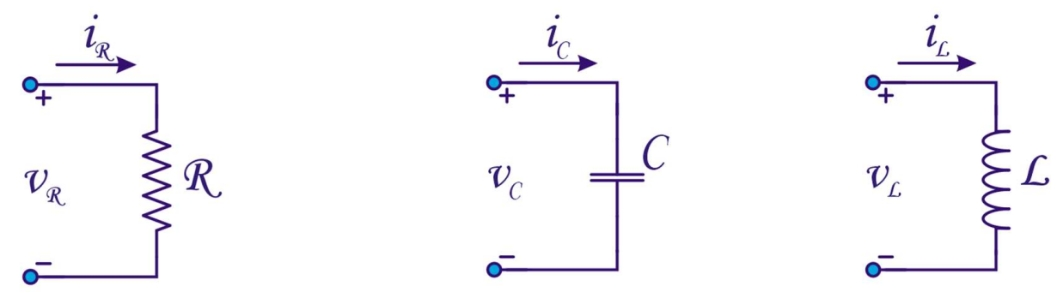
\includegraphics[width=14cm]{figures/ch00/passive.jpg}
	\caption{Resistor (left), capacitor (middle) and inductor (right)}
	\label{fig:passive}
\end{figure}


Les composants passifs linéaires les plus importants sont :
\begin{itemize}
	\item Une \emph{résistance} est un élément qui résiste à l'écoulement du courant en raison d'une tension appliquée. La relation courant-tension est :
	$$v_R = R\;i_R$$
	
	La résistance d'une résistance est mesurée en ohms ($\Omega$).
	\item Un \emph{condensateur} est un composant électronique passif qui stocke de l'énergie électrique dans un champ électrique. Il se compose de deux plaques conductrices séparées par un matériau isolant appelé diélectrique.\\
	Lorsqu'une tension est appliquée aux plaques d'un condensateur, une charge électrique $Q$ s'accumule sur les plaques, créant un champ électrique entre elles.
	
	La relation courant-tension est
	$$v_C  = \frac{Q}{C} = \frac{1}{C} \int i_C \; dt$$
	ou encore 
	$$i_C = C  \; \frac{dv_C}{dt}$$
	
	Un condensateur résiste à un changement soudain de tension à ses bornes. La capacité d'un condensateur est mesurée en farads ($F$).
	\item Une \emph{inductance} est un composant électronique passif qui stocke de l'énergie électrique dans un champ magnétique. Elle se compose d'une bobine de fil, souvent enroulée autour d'un noyau en un matériau magnétique tel que le fer ou la ferrite.\
	Lorsqu'un courant électrique circule dans une inductance, un champ magnétique est créé autour de la bobine. La force du champ magnétique est proportionnelle à la quantité de courant circulant dans la bobine. Lorsque le courant change, le champ magnétique change, ce qui induit une tension à travers la bobine qui s'oppose au changement de courant. Ainsi, une inductance résiste à un changement soudain de courant.
	La relation courant-tension est
	$$
	v_L = L  \;  \frac{di_L}{dt}
	$$
	ou encore
	$$
	i_L = \frac{1}{L}\int v_L  \;  dt
	$$
	L'inductance d'une inductance est mesurée en henry ($H$).
	
\end{itemize}

\begin{figure}[h!]
	\centering
	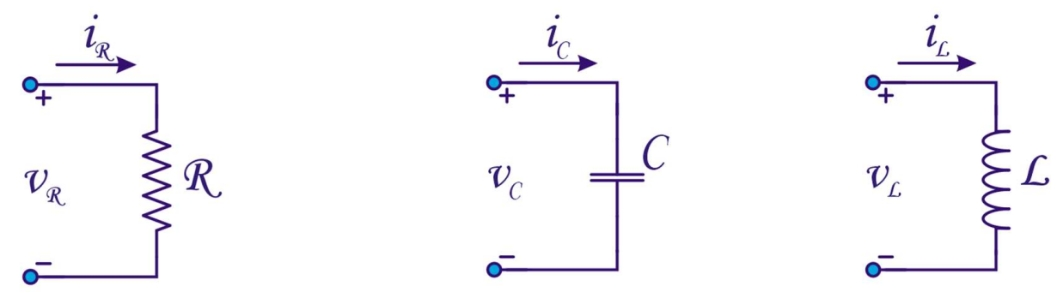
\includegraphics[width=14cm]{figures/ch00/passive.jpg}
	\caption{Résistance (à gauche), condensateur (au milieu) et inductance (à droite)}
	\label{fig:passive}
\end{figure}

\section{Lois de Kirchhoff}
\subsection{Loi des tensions de Kirchhoff}
La loi des tensions de Kirchhoff (LTV) stipule que la somme des différences de potentiel (tensions) autour d'une boucle fermée est nulle :
\begin{equation}
	\sum_{k=1}^n v_k = 0
	\label{eq:KVL}
\end{equation}
La LTV est en réalité une reformulation de la loi de Faraday $\nabla \times \vec{E} = -\frac{\partial B}{\partial t} = 0$, où l'on suppose que les champs magnétiques (variables dans le temps) sont confinés à chaque composant et que le champ dans la région extérieure au circuit est négligeable.

\begin{minipage}{.5\textwidth}
	\centering
	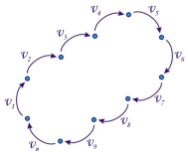
\includegraphics[width=5cm]{figures/ch00/kvl.jpg}
	\captionof{figure}{Loi des tensions de Kirchhoff}
	\label{fig:kvl}
\end{minipage}
\begin{minipage}{.5\textwidth}
	\centering
	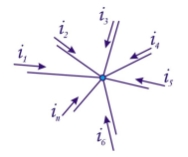
\includegraphics[width=5cm]{figures/ch00/kcl.jpg}
	\captionof{figure}{Loi des courants de Kirchhoff}
	\label{fig:kcl}
\end{minipage}%

\subsection{Loi des courants de Kirchhoff}
La loi des courants de Kirchhoff (LCK) affirme que dans un nœud d'un circuit électrique, la somme algébrique des courants est nulle :
\begin{equation}
	\sum_{k=1}^n i_k = 0
	\label{eq:KCL}
\end{equation}
ou de manière équivalente, que la somme des courants entrant dans ce nœud est égale à la somme des courants en sortant. La loi repose sur le fait qu'il n'y a pas d'accumulation de charges dans aucun nœud du réseau.

\subsection{Exemple}

Considérons le circuit de la figure \ref{fig:example1}. Avec KVL, on peut écrire :
$$
v_{in} = v_R + v_C = R \; i + v_C
$$
avec $i = C ; \frac{dv_C}{dt}$. L'équation pour trouver $v_C$ devient :
$$
v_{in} = RC \; \frac{dv_C}{dt} + v_C
$$
Si $v_{in}$ est soudainement allumé (par exemple, en fermant un interrupteur à $t=0$), alors $v_{in} = V_0 ; u(t)$ avec $u(t)$ la fonction échelon. On peut alors résoudre pour $v_C(t)$ :
\begin{align*}
	RC ; \frac{dv_C}{dt} + v_C &= V_0 \\
	\frac{dv_C}{dt} &= \frac{1}{RC} (V_0 - v_C) \\
	\frac{dv_C}{V_0 - v_C} &= \frac{dt}{RC} \\
	\int_0^{v_C} \frac{dv_C}{V_0 - v_C} &= \int_0^t \frac{dt}{RC} \\
	- \ln(V_0 - v_C) &= \frac{t}{RC} + K' \\
	v_C(t) &= V_0 - K e^{\frac{-t}{RC}}
\end{align*}
avec $K = V_0$ de telle sorte que $v_C(t=0) = 0$ :
$$
v_C(t) = V_0(1 - e^{\frac{-t}{RC}}) = V_0(1 - e^{-\frac{t}{T}})
$$

\begin{minipage}{.5\textwidth}
	\centering
	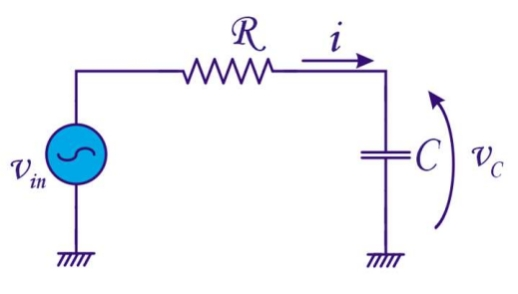
\includegraphics[width=6cm]{figures/ch00/example1.jpg}
	\captionof{figure}{}
	\label{fig:example1}
\end{minipage}
\begin{minipage}{.5\textwidth}
	\centering
	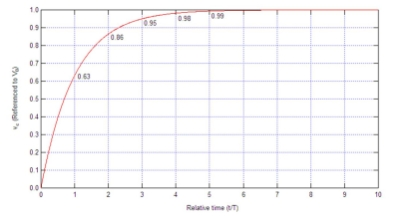
\includegraphics[width=9cm]{figures/ch00/first_order.jpg}
	\captionof{figure}{}
	\label{fig:first_order}
\end{minipage}%
\\Cette fonction est représentée dans la figure \ref{fig:first_order}. La tension $v_C$ augmente comme la réponse à un échelon d'un système du premier ordre, et atteint $63\%$ de la valeur finale après un temps caractéristique $T = RC$. Il faut $5T$ pour atteindre $99\%$ de la valeur finale.
\section{Représentation en fréquence}
\subsection{La transformation de Steinmetz}
Supposons qu'un signal sinusoïdal avec une fréquence $f = \omega/2\pi$ soit appliqué à un circuit ne contenant que des éléments linéaires. La théorie des systèmes linéaires nous enseigne alors que chaque courant et tension sera également une sinusoïde avec la même fréquence. Supposons que le courant dans un élément peut être écrit comme $I = I_0 \cos(\omega ; t) = Re{I_0 e^{j\omega t}}$. Dans ce cas, nous pouvons écrire :
\begin{itemize}
	\item Pour une résistance : $V_R = R ; I_R$
	\item Pour un condensateur : $V_C = \frac{1}{C} \int I_L \; dt = \frac{1}{C} \int I_0 e^{j\omega t} \; dt = \frac{1}{j\omega C} I_0 e^{j\omega t} = \frac{1}{j\omega C} \; I_C$
	\item Pour une inductance : $V_L = L \frac{dI_L}{dt} = L \frac{d(I_0 e^{j\omega t})}{dt} = j \omega L ; I_0 e^{j\omega t} = j \omega L ; I_L$
\end{itemize}
Ces relations sont la représentation en phaseur d'un signal sinusoïdal, ou les transformations de Steinmetz. Elles sont résumées dans la figure \ref{fig:steinmetz}.

\begin{figure}[h!]
	\centering
	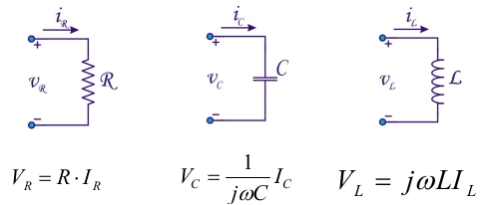
\includegraphics[width=10cm]{figures/ch00/steinmetz.jpg}
	\caption{}
	\label{fig:steinmetz}
\end{figure}

De cela, nous concluons que pour chaque élément, nous pouvons écrire:
$$
V = Z \cdot I
$$
où $Z$ est l'\emph{impédance complexe} de l'élément : $R$ pour une résistance, $\frac{1}{j\omega C}$ pour un condensateur et $j\omega L$ pour une bobine.\
Nous définissons également d'autres paramètres de circuit : $Y = \frac{1}{Z}$ comme l'\emph{admittance} telle que $I = Y \cdot V$, et $G = \frac{1}{R}$ comme la \emph{conductance} (mesurée en siemens ou A/V).

\subsection{La transformation de Laplace}
\label{sec:laplace}

La représentation phasorique ou la transformée de Steinmetz n'est possible que pour des signaux sinusoïdaux. Cette condition est parfois trop restrictive et nous avons besoin d'autres méthodes d'analyse. L'une de ces méthodes, qui est valable pour des signaux arbitraires $x(t)$, est la transformée de Laplace (unilatérale) $X(s)$, définie comme :
$$
\mathcal{L}[x(t)] = X(s) = \int_{t = 0}^{+\infty} e^{-st} x(t) dt
$$
avec $s$ la variable de Laplace complexe : $s = \sigma + j\omega$. Comme exemple, calculons $\mathcal{L}[\frac{dx(t)}{dt}]$ :
\begin{align*}
	\mathcal{L}[\frac{dx(t)}{dt}] &= \int_{t = 0}^{+\infty} e^{-st} \frac{dx}{dt} dt \
	&= e^{-st} x(t) |{t = 0}^{+\infty} - \int{t = -\infty}^{+\infty} x(t) \frac{d(e^{-st})}{dt} dt \
	&= \int_{t = 0}^{+\infty} s;x(t) e^{-st} dt - x(0^+)\
	&= s X(s) - x(0^+)
\end{align*}
Lorsque nous supposons que $x(0^+) = 0$, nous trouvons que $\mathcal{L}[\frac{dx(t)}{dt}] = s X(s)$. Un système linéaire avec une entrée $x(t)$ et une sortie $y(t)$ peut être décrit par une équation différentielle linéaire d'ordre supérieur :
\begin{align*}
	y(t) &= a_0 x(t) + a_1 \frac{dx}{dt} + a_2 \frac{d^2 x}{dt^2} + \ldots + b_1 \frac{dy}{dt} + b_2 \frac{d^2 y}{dt^2} + \ldots\
	\Rightarrow \frac{Y(s)}{X(s)} &= \frac{a_0 + a_1 s + a_2 s^2 + \ldots}{1 - b_1 s - b_2 s^2 - \ldots}
\end{align*}
Ainsi, la transformée de Laplace de tout système linéaire peut être écrite comme le rapport de deux polynômes en $s$. Supposons que nous avons un système du premier ordre :
\begin{align}
	\frac{dy}{dt} &= \alpha ; y(t) + \beta ; x(t)
	\label{eq:first_order}
\end{align}
Si il n'y avait pas d'entrée $x(t)$, la solution serait :
$$
y(t) = C e^{\alpha t}
$$
Cette sortie reste finie pour $t \rightarrow \infty$ uniquement lorsque $\alpha \le 0$. C'est le critère de stabilité pour un système du premier ordre.\
Si nous prenons la transformée de Laplace de l'équation \ref{eq:first_order}, nous trouvons :
\begin{align*}
	s Y(s) &= \alpha ; Y(s) + \beta ; X(s) \
	\Rightarrow \frac{Y(s)}{X(s)} &= \frac{\beta}{s - \alpha}
\end{align*}
Les racines du dénominateur sont les \emph{pôles} de la transformée de Laplace. Dans ce cas, nous avons un seul pôle en $s = \alpha$. Nous avons déjà déterminé que le système est stable lorsque $\alpha \le 0$. C'est une règle générale : \textbf{un système $S(s)$ est stable si tous ses pôles se trouvent dans le demi-plan gauche du plan complexe (LHP)}, c'est-à-dire si leur partie réelle est négative.\
Nous utilisons principalement la représentation de Steinmetz car les signaux que nous considérons sont principalement sinusoïdaux. Cependant, dans certains cas, nous aurons besoin de la transformée de Laplace.

\subsection{Combinaisons en série et en parallèle}

Deux impédances sont en série lorsque le même courant $I$ les traverse, comme illustré sur la figure \ref{fig:series}. La chute de tension sur les deux est donc $Z_1 \cdot I + Z_2 \cdot I = (Z_1 + Z_2) \cdot I = Z \cdot I$ avec $Z = Z_1 + Z_2$ la combinaison en série de $Z_1$ et $Z_2$.

\begin{minipage}{.5\textwidth}
	\centering
	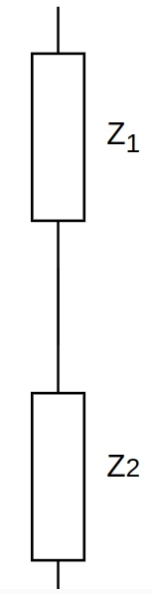
\includegraphics[height=6cm]{figures/ch00/series.jpg}
	\captionof{figure}{}
	\label{fig:series}
\end{minipage}
\begin{minipage}{.5\textwidth}
	\centering
	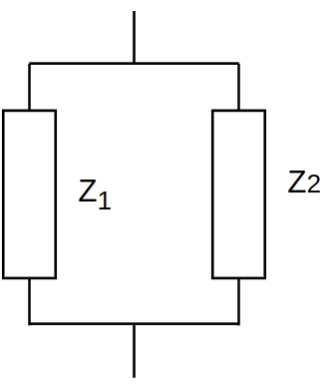
\includegraphics[width=4cm]{figures/ch00/parallel.jpg}
	\captionof{figure}{}
	\label{fig:parallel}
\end{minipage}%

Deux impédances sont en parallèle lorsqu'une même tension $V$ est appliquée à leurs bornes, comme illustré sur la figure \ref{fig:parallel}. Le courant à travers $Z_1$ est $V/Z_1$ et le courant à travers $Z_2$ est $V/Z_2$. Le courant total $I$ à travers les deux est donc $V/Z_1 + V/Z_2 = V \big(\frac{1}{Z_1} + \frac{1}{Z_2} \big) = \frac{V}{Z}$ avec $Z = \big(\frac{1}{Z_1} + \frac{1}{Z_2} \big)^{-1}$ la combinaison en parallèle de $Z_1$ et $Z_2$.

\subsection{Théorème de Millman}
Le théorème de Millman est dérivé de la loi de Kirchhoff sur les courants et permet de calculer la tension dans un nœud en fonction des tensions dans les nœuds voisins (voir figure \ref{fig:millman}):
\begin{equation}
	v_0 = \frac{\sum_{i=1}^n Y_i v_i + I_{eq}}{\sum_{i=1}^n Y_i}
	\label{eq:millman}
\end{equation}
avec $Y_i$ la conductance de chaque élément.
\begin{figure}[h!]
	\centering
	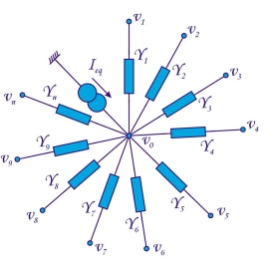
\includegraphics[width=6cm]{figures/ch00/millman.jpg}
	\caption{}
	\label{fig:millman}
\end{figure}
\\On peut déduire ce théorème en appliquant la loi de KCL au noeud $0$:
\begin{align*}
	\sum_{i = 1}^n I_n = \sum_{i = 1}^n Y_i(v_i - v_0) + I_{eq} = 0 \\
	\Rightarrow v_0 \; \sum_{i = 1}^n Y_i = \sum_{i = 1}^n Y_i\;v_i  + I_{eq} \\
	\Rightarrow v_0  = \frac{\sum_{i=1}^n Y_i v_i + I_{eq}}{\sum_{i=1}^n Y_i} 
\end{align*}
La tension dans le noeud $0$ est donc la moyenne pondérée des tensions environnantes, avec les conductances comme poids.

\subsection{Diagramme de Bode}
Appliquons les concepts de cette section au problème de la figure \ref{fig:example1}. Comme nous avons supposé que tous les signaux sont sinusoïdaux, nous posons que $v_{in} = V_0 e^{j\omega t}$. Par conséquent:
\begin{align*}
	V_{in} &= I \cdot R + \frac{1}{j \omega C} I \\
	\Rightarrow I &= \frac{j \omega C}{1 + j \omega RC} ; V_{in}\\
	\text{et} \quad V_C &= \frac{1}{1 + j \omega RC} ; V_{in}
\end{align*}
Nous pouvons donc conclure que:
\begin{align*}
	\frac{V_C}{V_{in}} &= \frac{1}{1 + j \omega RC} \\
	&= \frac{1}{\sqrt{1 + \omega^2 T^2}} e^{-j \phi}
\end{align*}
avec $\phi = \text{atan}(\omega ; T)$. Notez que nous ne trouvons aucune information sur la réponse transitoire comme précédemment, mais nous trouvons comment le circuit se comporte en \emph{régime harmonique permanent} (RHP).\
Le rapport $\frac{V_C}{V_{in}}$ est appelé \emph{transmittance} $H(\omega)$ et il a une amplitude $A = |T(\omega)|$ et une phase $\phi$. Lorsque nous traçons $20 \log(A)$ [dB] en fonction de $\log(\omega)$, nous trouvons la courbe de Bode:

$$
20 \log(A) = -20 \; \frac{1}{2} \; \log_{10}(1 + \omega^2 T^2)
$$
À partir de cette expression, nous déduisons que:
\begin{itemize}
	\item Lorsque $\omega T \ll 1$, $20 \log_{10}(A) \approx 20 \log_{10}(1) = 0$.
	\item D'autre part, lorsque $\omega T \gg 1$, $20 \log_{10}(A) \approx -20 \log_{10}(\omega T)$ et $|H(\omega)|$ diminue de $20$ dB pour chaque augmentation de $\omega$ d'un facteur de $10$ ($-20$ dB par décade).
\end{itemize}

En règle générale, toute transmittance $T(\omega)$ peut être écrite sous la forme :
$$
T(\omega) = A_0 \frac{(1 + j \omega T_{n+1}) \ldots (1 + j \omega T_{p})}{(1 + j \omega T_{1}) \ldots (1 + j \omega T_{n})}
$$
Chaque terme individuel est égal à $1$ si $\omega \ll 1/T_i$ ou égal à $j \omega T_i$ si $\omega \gg 1/T_i$. Par conséquent, une courbe de Bode peut être construite approximativement en suivant quelques règles simples : lorsque l'on rencontre une pulsation critique $\omega = 1/T$ dans le numérateur (un \emph{zéro}) ou dans le dénominateur (un \emph{pôle}), la courbe va :
\begin{itemize}
	\item décroître de $20$ dB par décade pour un pôle,
	\item augmenter de $20$ dB par décade pour un zéro,
\end{itemize}
Des règles similaires existent pour la phase $\phi$ du signal : chaque pôle introduit un décalage de $-\frac{\pi}{2}$, chaque zéro crée un décalage de $+\frac{\pi}{2}$. Notez que ces règles ne produisent qu'une estimation des courbes de Bode ; le tracé réel présentera un comportement plus compliqué, surtout lorsque les pôles sont complexes.\
Un exemple basé sur la figure \ref{fig:example1} est donné dans la figure \ref{fig:bode1}. Pour un système du premier ordre comme celui-ci, la coupure à -$3$ dB est atteinte à $\omega = \omega_0$, la pulsation critique.
\begin{figure}[h!]
	\centering
	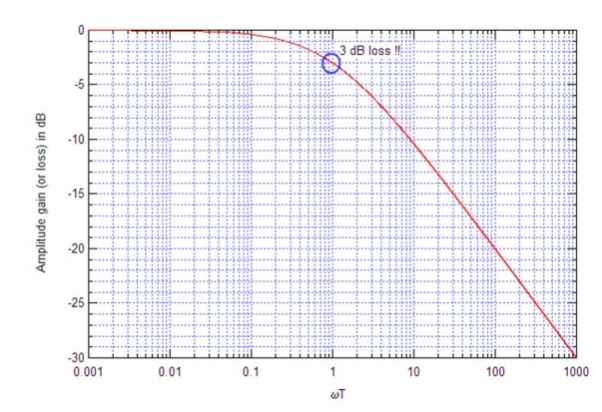
\includegraphics[width=10cm]{figures/ch00/bode.jpg}
	\caption{}
	\label{fig:bode1}
\end{figure}

\section{Transformations de circuits}
\subsection{Théorème de Thévenin}
Le théorème de Thévenin stipule qu'un réseau électrique linéaire à deux bornes peut être remplacé aux bornes A-B par une combinaison équivalente d'une source de tension $E_{Th}$ en série avec une impédance $Z_{Th}$. Deux circuits sont équivalents s'ils ont la même relation tension-courant à leurs bornes. Cette idée est illustrée dans la figure \ref{fig:thevenin}, où les éléments du circuit dans le nuage bleu sont remplacés par la source et l'impédance à droite.

\begin{itemize}
	\item La tension équivalente $E_{Th}$ est la tension obtenue aux bornes A-B du réseau avec les bornes A-B en circuit ouvert.
	\item L'impédance équivalente $Z_{Th}$ est l'impédance que le circuit entre les bornes A et B aurait si toutes les sources de tension idéales du circuit étaient remplacées par un court-circuit et toutes les sources de courant idéales étaient remplacées par un circuit ouvert.
\end{itemize}

\begin{minipage}{.5\textwidth}
	\centering
	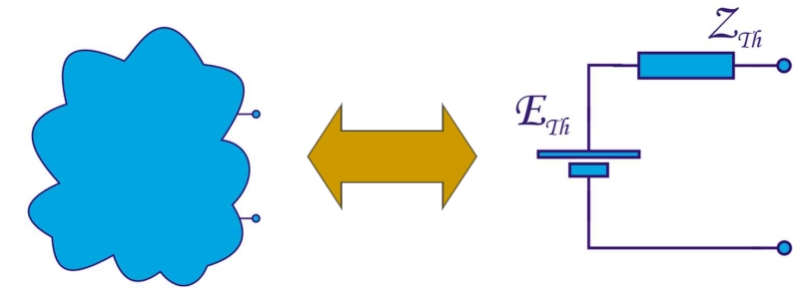
\includegraphics[width=7cm]{figures/ch00/thevenin.jpg}
	\captionof{figure}{Thévenin equivalent}
	\label{fig:thevenin}
\end{minipage}
\begin{minipage}{.5\textwidth}
	\centering
	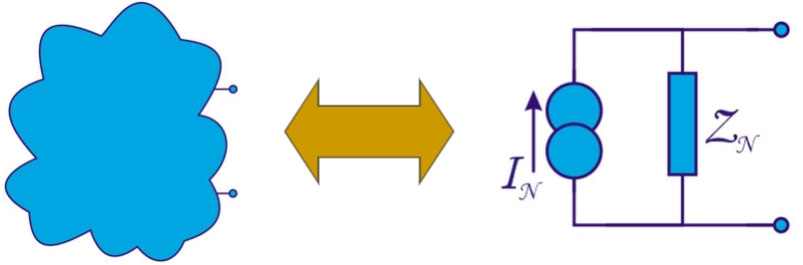
\includegraphics[width=7cm]{figures/ch00/norton.jpg}
	\captionof{figure}{Norton equivalent}
	\label{fig:norton}
\end{minipage}%

\subsection{Le théorème de Norton}
Le théorème de Norton nous indique comment remplacer un réseau linéaire par une source de courant $I_N$ en parallèle avec une impédance $Z_N$, comme illustré dans la figure \ref{fig:norton}. C'est le dual du théorème de Thévenin.
\begin{itemize}
	\item Le courant de Norton $I_N$ est calculé comme le courant qui circule aux bornes d'un court-circuit (résistance nulle entre les bornes de sortie).
	\item L'impédance $Z_N$ est trouvée en calculant la tension de sortie produite sans résistance connectée aux bornes; de manière équivalente, c'est la résistance entre les bornes avec toutes les sources de tension (indépendantes) court-circuitées et toutes les sources de courant (indépendantes) circuit ouvert. Cela équivaut à calculer la résistance de Thévenin : $Z_{Th} = Z_{N}$.
\end{itemize}
De plus, la tension de sortie générée par la source de Norton avec les bornes de sortie ouvertes est égale à la tension de Thévenin : $E_{Th} = Z_{N} ; I_N$.

\subsection{Deux Ports}
Certains circuits ont deux noeuds d'accès: une entrée et une sortie. Nous supposons que le port est unilatéral: les signaux transitent de l'entrée à la sortie et ne reviennent pas. Nous modélisons l'entrée comme une impédance $Z_i$ et la sortie comme un circuit équivalent Thévenin ou Norton - voir la figure \ref{fig:two_port}. Notez comment les sources de courant et de tension dépendent toutes deux de la tension d'entrée.
\begin{figure}[h!]
	\centering
	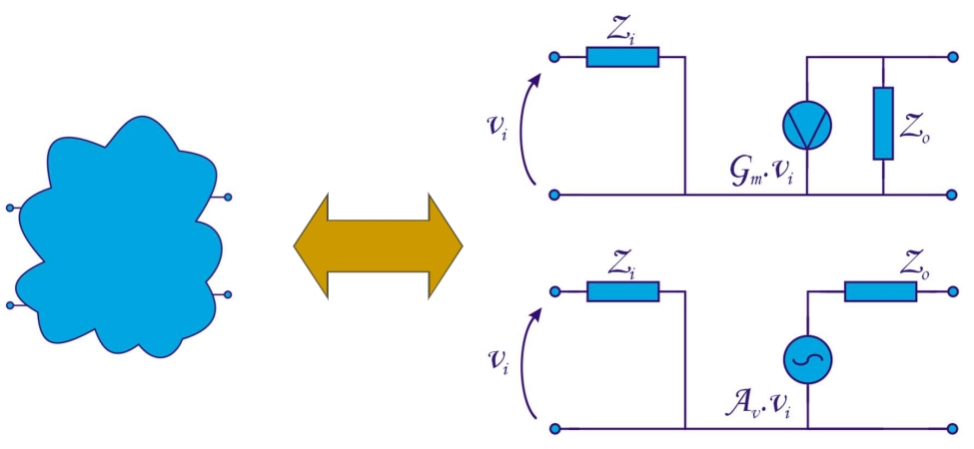
\includegraphics[width=12cm]{figures/ch00/two_port.jpg}
	\caption{}
	\label{fig:two_port}
\end{figure}
Les différents éléments ont des noms:
\begin{itemize}
	\item $Z_i$: l'impédance d'entrée,
	\item $Z_o$: l'impédance de sortie,
	\item $G_m$: la transconductance,
	\item $A_v$: le gain de tension.
\end{itemize}
Ils peuvent être calculés de la manière suivante:
\begin{itemize}
	\item $Z_i$: appliquer une tension d'entrée $V_i$, calculer le courant d'entrée $I_i$. Ensuite, $Z_i = \frac{V_i}{I_i}$;
	\item $Z_o$: éliminer la transconductance en reliant l'entrée à la masse: $V_i = 0$, appliquer une tension $V_o$ à la sortie et calculer le courant de sortie $I_o$. Ensuite, $Z_o = \frac{V_o}{I_o}$.
	\item $G_m$: court-circuiter la sortie de sorte qu'aucun courant ne passe à travers $Z_o$. Appliquer une tension d'entrée $V_i$ et calculer le courant de sortie $I_o$. Ensuite, $G_m = \frac{I_o}{V_i}$.
	\item $A_v$: garder la sortie ouverte. Appliquer une tension d'entrée $V_i$ et calculer la tension de sortie $V_o$. Ensuite, $A_v = \frac{V_o}{V_i}$.
\end{itemize}


\subsection{Circuits en cascade}

Lorsque plusieurs circuits sont connectés en cascade, on parle de circuits en cascade. Ils se composent généralement de :

\begin{itemize}
	\item Une source, telle qu'une antenne, un générateur de signal ou un microphone, que l'on modélise comme une source de courant $i_s$ ou de tension $v_s$, en parallèle ou en série avec une impédance de sortie $Z_s$.
	\item Un étage intermédiaire tel qu'un amplificateur ou un filtre qui transforme réellement le signal. Cet étage a une impédance d'entrée $Z_i$, une impédance de sortie $Z_o$, un gain de tension $A_v$ ou une transconductance $G_m$.
	\item Une charge, qui peut être un PC, un oscilloscope, un haut-parleur, ... Nous modélisons cela comme une impédance de charge $Z_l$.
\end{itemize}

Cette configuration est illustrée dans la figure \ref{fig:cascade}.

Si nous ne faisons pas attention, chaque étage influencera l'étage précédent ou suivant. Nous pouvons calculer la relation entre le courant de source $i_s$ et la tension de charge $v_l$ dans la figure \ref{fig:cascade} :

\begin{itemize}
	\item La tension $v_i$ aux bornes de $Z_i$ est :
	$$v_i = i_s\;(Z_s || Z_i) = \frac{Z_s Z_i}{Zs+Z_i} i_i$$
	et pas simplement $i_s;Z_s$. L'étage intermédiaire charge l'étage source.
	\item La tension de charge $v_l$ aux bornes de $Z_l$ est :
	$$v_l = - G_m (Z_o || Z_l) v_i = -G_m \frac{Z_o Z_l}{Z_o + Z_l} v_i$$ 
	et pas simplement $-G_m Z_l v_i$. L'impédance de sortie de l'étage intermédiaire s'ajoute à la charge.
	\item Cela signifie que la tension du signal disponible en sortie est :
	$$v_l = -G_m Z_o  \frac{Z_l}{Z_o + Z_l} \frac{Z_i}{Zs+Z_i} Z_s i_i = \frac{Z_l}{Z_o + Z_l} \frac{Z_i}{Zs+Z_i} A_v v_s$$
\end{itemize}
Idéalement, cela devrait être $v_l = - A_v v_s$. À partir de cela, nous pouvons conclure que $Z_i \rightarrow \infty$ et que $Z_o \rightarrow 0$ pour se rapprocher du comportement idéal. Nous devons concevoir pour avoir une impédance d'entrée élevée et une impédance de sortie faible.
\part{Composantes}
\chapter{Théorie des Semi-conducteurs et des Solides}
%\section{Chapter Overview}
Dans ce chapitre, nous aborderons le concept de semi-conducteur. Nous décrirons le type de matériau que cela représente, basé sur le concept de bandes d'énergie. Sous forme solide, un semi-conducteur comme le silicium forme un cristal, donc une attention particulière est portée au comportement des électrons dans un cristal. Le nombre de porteurs de charge dans un semi-conducteur (qui peuvent être des électrons, comme dans un métal, ou des trous, qui n'existent pas dans un métal) est calculé. Pour augmenter le nombre de porteurs, nous dopons le semi-conducteur avec des impuretés. Ensuite, nous considérons les phénomènes de transport les plus importants dans les semi-conducteurs, à savoir la dérive et la diffusion. Enfin, nous discutons de la génération et de la recombinaison de paires électron-trou et établissons les équations de continuité.
\section{Les Semi-conducteurs}
Nous appelons semi-conducteurs les éléments de la quatrième colonne de la table périodique. Des exemples sont le carbone (C), le silicium (Si) et le germanium (Ge). Ces éléments ont 4 électrons sur leur couche externe et ont tendance à former 4 liaisons covalentes avec les atomes voisins pour obtenir une structure octet stable. En se liant, ils forment un motif régulier appelé cristal.\\
Le silicium, l'atome de semi-conducteur le plus couramment utilisé en électronique, a une couche externe ($n=3$) avec un orbitale $3s^2$ complètement rempli et un orbitale $3p^2$ partiellement rempli. Pour former des liaisons, les orbitales de la couche externe interagissent et subissent une hybridation $sp^3$. La conséquence est que les 4 liaisons covalentes sont uniformément espacées dans l'espace, formant des liaisons d'environ $109^{\circ}$ les unes avec les autres.\\
La partie gauche de la figure \ref{fig:crystal} montre une seule cellule de la structure cristalline du silicium. Les points bleus représentent un seul atome de silicium, avec des liaisons covalentes à $4$ atomes voisins. La figure de droite montre une représentation simplifiée en 2 dimensions du même cristal.\\
Parfois, un élément composé peut également être un semi-conducteur. L'arséniure de gallium (GaAs) est un composé composé d'atomes de gallium et d'arsenic. C'est un semi-conducteur composé III-V, ce qui signifie qu'il est composé d'éléments des groupes III et V de la table périodique.

\begin{figure}[htbp]
	\centering
	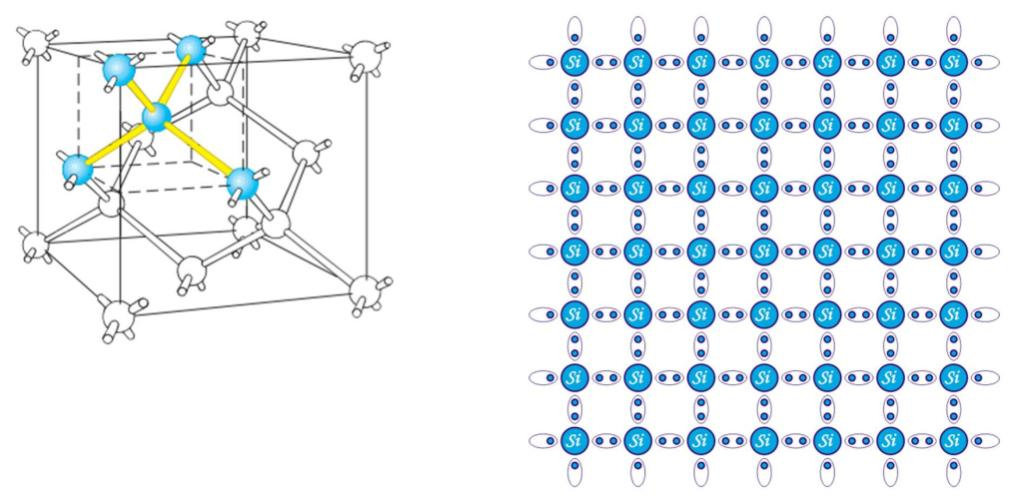
\includegraphics[width=12cm]{figures/ch01/crystal.jpg}
	\caption{Silicon crystal (left) - schematic representation (right)}
	\label{fig:crystal}
\end{figure} 

\subsection{Structure de bande}
Lorsque les atomes sont très éloignés, ils ne s'influencent pas mutuellement et nous pouvons trouver leur fonction d'onde $\Psi(x, t)$ en résolvant l'équation de Schrödinger pour un seul électron en orbite autour d'un noyau fixe. Cela résulte dans le spectre d'énergie discret bien connu associé à chaque fonction d'onde. Cependant, lorsque les atomes se rapprochent, leurs électrons dans la couche externe commencent à interagir les uns avec les autres. Selon le principe d'exclusion de Pauli, ils ne peuvent plus occuper les mêmes niveaux d'énergie.\\
Supposons que $N$ atomes de Si sont initialement très éloignés, et nous les rapprochons avec pour objectif de former un cristal. Nous avons donc $2N$ électrons au niveau d'énergie de l'orbitale $3s$, et $2N$ électrons dans l'orbitale $3p$, où il y a $6N$ niveaux disponibles. Lorsque les atomes sont suffisamment proches, ils interagissent et les niveaux d'énergie doivent légèrement descendre ou monter pour être conformes au principe d'exclusion de Pauli. Les niveaux sont toujours discrets, mais étant donné que $N$, le nombre d'atomes dans le cristal, est un nombre énorme ($N \approx 10^{20}$ atomes par cm$^3$), nous pouvons considérer la bande d'énergie résultante comme un spectre continu (voir la figure \ref{fig:bandstructure}). À partir d'un certain espacement de réseau, les bandes $3s$ et $3p$ fusionnent pour former une seule bande. Lorsque les atomes se rapprochent suffisamment pour former un cristal comme dans la figure \ref{fig:crystal}, nous observons que les bandes se séparent à nouveau. À la distance interatomique dans le réseau cristallin ($5.43 \AA$ pour le silicium), il y a une \emph{bande de valence} avec des énergies jusqu'à une énergie $E_V$ et une \emph{bande de conduction} avec des énergies supérieures à $E_C > E_V$. Entre les bandes se trouve une plage interdite où aucun électron ne peut exister. Cette plage est appelée \emph{gap} de bande et la différence entre $E_C$ et $E_V$ est l'\emph{énergie de gap} $E_g$.

\begin{figure}[h!]
\centering
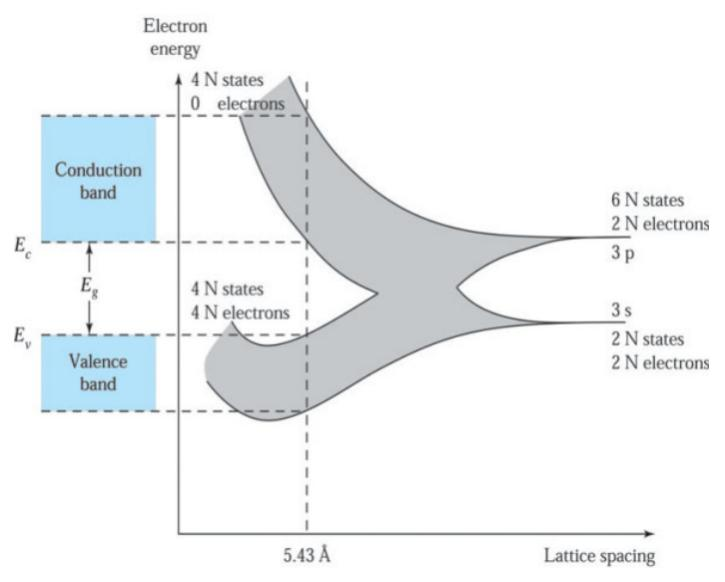
\includegraphics[width=12cm]{figures/ch01/bandstructure.jpg}
\caption{Band structure formation}
\label{fig:bandstructure}
\end{figure} 

\section{Électrons et trous}
À une température de $0$ K, tous les $4N$ électrons se trouvent dans la bande de valence. Cela signifie qu'ils font tous partie d'une liaison covalente entre deux atomes de silicium. Cependant, à mesure que la température augmente, les électrons obtiennent plus d'énergie thermique et certains d'entre eux peuvent rompre la liaison covalente et devenir des électrons libres qui peuvent se déplacer à travers le cristal. Ils ont acquis suffisamment d'énergie pour passer de la bande de valence à la bande de conduction. Lorsqu'une liaison covalente est rompue, l'électron laisse derrière lui une position vide. Cette position libre peut être occupée par un autre électron provenant d'une autre liaison électronique. Ce mécanisme est illustré sur la figure \ref{fig:breakingbond}. Une position vide dans une liaison est appelée un \emph{trou}. Puisque les électrons sautant d'un trou à l'autre font bouger le trou dans le cristal, nous pouvons considérer un trou comme une autre particule en mouvement, avec une charge positive $+q$.\\
Il existe également d'autres mécanismes en plus de l'agitation thermique qui peuvent fournir suffisamment d'énergie à un électron pour qu'il saute de la bande de valence à la bande de conduction, comme un photon qui frappe avec une énergie $E$ suffisamment élevée (donc une fréquence $\nu$, puisque $E = \hbar \nu$). Le fond de la bande de conduction $E_C$ correspond à l'énergie potentielle d'un électron, tout comme le sommet de la bande de valence $E_V$ correspond à l'énergie potentielle d'un trou.

\begin{figure}[h!]
\centering
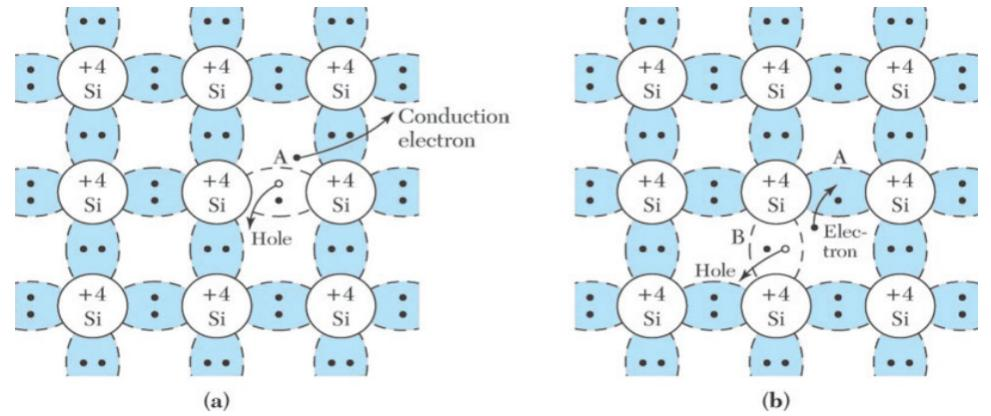
\includegraphics[width=12cm]{figures/ch01/breakingbond.jpg}
\label{fig:breakingbond}
\caption{Creation of electron hole pair by breaking of covalent bonds}
\end{figure} 

Lorsque l'on considère différentes directions dans le réseau cristallin, la structure de bande diffère car la distance interatomique dépend de la direction. La direction de propagation d'une fonction d'onde est déterminée par son vecteur d'onde $\vec{k}$, et $k$ est directement lié à l'impulsion $p$ par la relation :
$$\vec{p} = \hbar \vec{k}$$
C'est pourquoi ces \emph{diagrammes de bande} sont généralement tracés en fonction de l'énergie $E$ en fonction de l'impulsion $p$. La figure \ref{fig:indirectbandgap} montre les diagrammes de bande pour le silicium (à gauche) et le GaAs (à droite).\
Ces figures montrent que pour certains semi-conducteurs, comme le GaAs, le minimum de la bande de conduction se situe dans la même direction que le maximum de la bande de valence. Ces semi-conducteurs sont appelés semi-conducteurs à \emph{bande interdite directe}. D'autres, comme le silicium, ont des directions différentes pour ces deux points et sont donc appelés semi-conducteurs à \emph{bande interdite indirecte}.

\begin{figure}[h!]
\centering
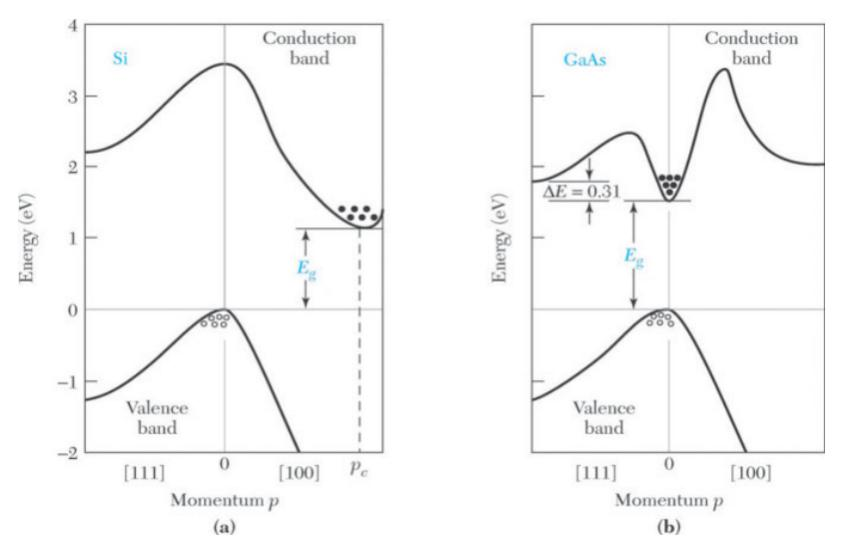
\includegraphics[width=12cm]{figures/ch01/indirectbandgap.jpg}
\caption{Band diagrams: (a) Si and (b) GaAs} 
\label{fig:indirectbandgap}
\end{figure} 

\subsection{Masse effective}
Un électron libre - non entravé par d'autres particules et leurs fonctions potentielles - a une masse $m_0 = 9,11 \; 10^{-31}$ kg. Cependant, dans un cristal, les électrons de la bande de conduction sont influencés par les noyaux et les autres électrons. Pour déterminer leur comportement, nous devrions résoudre l'équation de Schrödinger pour toutes ces particules. À la place, nous introduisons le concept de masse effective, qui peut être considérée comme la masse apparente d'une particule (électron ou trou) dans un cristal.\\
Chaque fonction d'onde a une vitesse de groupe $v_g = \frac{d \omega}{dk}$ et puisque $E = \hbar \omega$, nous avons $v_g = \frac{1}{\hbar}\frac{dE}{dk}$. Mais comme l'augmentation d'énergie $dE$ de la particule peut être considérée comme le résultat du travail $dW$ effectué par une force $F$ via la relation $dW = F dl = F v_g dt$ où $dl$ est le déplacement en temps $dt$, nous pouvons simplifier cette relation en $\frac{dk}{dt} = \frac{F}{\hbar}$.\\
Si une particule subit une variation de vitesse de groupe - une accélération $a$ - nous pouvons affirmer que:
\begin{equation} \label{eq1}
\begin{split}
a &= \frac{dv_g}{dt} = \frac{1}{\hbar}\frac{d}{dt}\frac{dW}{dk} \\
  &= \frac{1}{\hbar}\frac{d^2 W}{dk^2}\frac{dk}{dt} \\
  &= \frac{1}{\hbar^2}\frac{d^2 W}{dk^2}F
\end{split}
\end{equation}

Cela donne une relation entre la force appliquée $F$ et l'accélération résultante $a$. Ainsi, selon la deuxième loi de Newton $F = ma$, nous pouvons interpréter la constante de proportionnalité comme la masse effective de la particule:
$$
m^* = \hbar^2 \Big[\frac{d^2 W}{dk^2}\Big]^{-1}
$$
La masse effective d'un électron ou d'un trou est donc déterminée par la courbure locale de la relation $E-k$ dans le diagramme de bande. À partir de la figure \ref{fig:indirectbandgap}, nous voyons que pour le silicium, la courbure de la bande de conduction est plus élevée que celle de la bande de valence. Par conséquent, la masse effective $m_e^*$ d'un électron sera plus petite que celle d'un trou $m_h^*$.

\subsection{Nombre de porteurs}
Nous pouvons calculer la concentration d'électrons et de trous dans le silicium pur en utilisant la statistique quantique. La distribution des fermions (comme les électrons) est déterminée par la distribution de Fermi-Dirac :
$$
F(E) = \frac{1}{1-e^{(E-E_F)/kT}}
$$
qui donne la probabilité qu'à la température $T$, un électron occupe le niveau d'énergie $E$. $E_F$ est le niveau de Fermi, un niveau de référence où la probabilité d'occupation est exactement de moitié, et $k$ est la constante de Boltzmann (à ne pas confondre avec le nombre d'onde $k$).\\
Nous considérons également le nombre d'états autorisés à un niveau d'énergie $E$. Nous savons déjà que entre $E_V$ et $E_C$, aucun état n'est disponible car c'est la région de la bande interdite. Pour respectivement les électrons dans la bande de conduction et les trous dans la bande de valence, nous avons que :
\begin{equation} 
\begin{split}
N_C(E)  &= \frac{4 \pi}{\hbar} (2 m_e^*)^{3/2} (E - E_C)^{1/2} \\
N_V(E)  &= \frac{4 \pi}{\hbar} (2 m_h^*)^{3/2} (E_V - E)^{1/2}
\end{split}
\end{equation}
où $N_C(E)$ et $N_V(E)$ représentent la densité d'états par unité de volume dans la bande de conduction et la bande de valence.\
Pour calculer la densité de porteurs, nous multiplions la densité d'états par la probabilité qu'un état soit occupé, et intégrons sur les niveaux d'énergie pertinents. Nous notons $n$ pour le nombre d'électrons dans la bande de conduction, et $p$ pour le nombre de trous dans la bande de valence :
\begin{equation}
	\begin{split}
		n = \int_{E_C}^{\infty} N_C(E) F_e(E) dE\\
		p = \int_{-\infty}^{E_V} N_V(E) F_h(E) dE
		\label{eq:carrier_density}
	\end{split}
\end{equation}
Puisque $E_C$ et $E_V$ sont tous deux suffisamment éloignés du niveau de Fermi, nous pouvons simplifier la distribution de Fermi-Dirac et obtenir une distribution de Boltzmann standard :
\begin{equation} 
\begin{split}
F_e(E) \approx e^{-(E-E_F)/kT}\text{ if }E-E_F \gg kT \\
F_h(E) \approx e^{(E-E_F)/kT}\text{ if }E-E_F \ll kT 
\label{eq:boltzmann_simple}
\end{split}
\end{equation}
En substituant \ref{eq:boltzmann_simple} dans \ref{eq:carrier_density}, on obtient :
\begin{equation} 
\begin{split}
n = N_C \; e^{-(E_C-E_F)/kT} \text{ with } N_C = \ldots\\
p = N_V \; e^{-(E_F-E_V)/kT} \text{ with } N_V = \ldots
\label{eq:carrier_density2}
\end{split}
\end{equation}

La figure \ref{fig:carrierdensity} représente le schéma de bande, la densité d'états $N(E)$, la distribution des porteurs $F(E)$ et les résultats finaux.

\begin{figure}[h!]
\centering
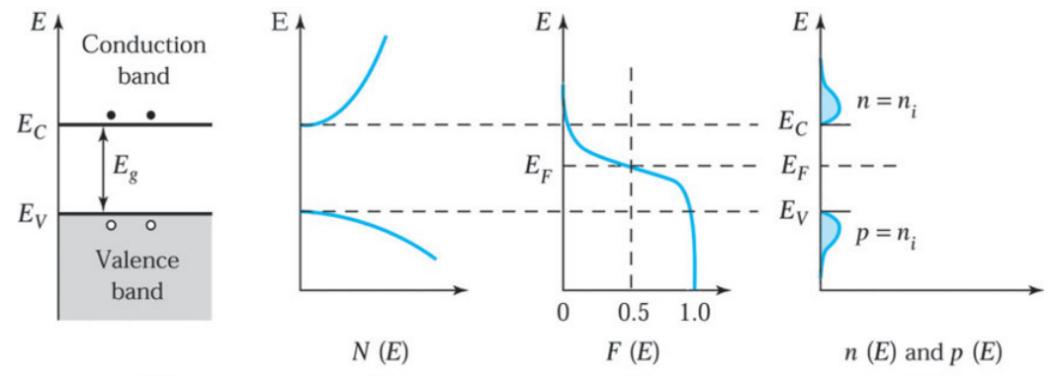
\includegraphics[width=12cm]{figures/ch01/carrierdensity.jpg}
\caption{Carrier density} 
\label{fig:carrierdensity}
\end{figure} 


Dans le silicium pur, chaque électron dans la bande de conduction donne naissance à un trou dans la bande de valence - d'où $n = p$ et $E_F$ se situe presque à mi-chemin entre $E_V$ et $E_C$ (la petite différence est due à une différence de masse effective entre les trous et les électrons). On dit que $n = p = n_i$, la densité de porteurs intrinsèques. En général, à température ambiante, $n \approx 10^{10}/cm^3$. Si nous multiplions les équations pour $n$ et $p$, le niveau de Fermi disparaît :
\begin{equation}
n p = n_i^2 = N_C \; e^{-(E_C-E_F)/kT} \; N_V \; e^{-(E_F-E_V)/kT} = N_C N_V \; e^{-E_g/kT}
\label{eq:np}
\end{equation}
\section{Impuretés donneuses et accepteuses}
La densité de porteurs intrinsèques $n_i$ est assez faible, et le silicium pur est un mauvais conducteur. Cependant, nous pouvons augmenter le nombre de porteurs (soit des trous, soit des électrons) avec un processus appelé \emph{dopage}. Le dopage consiste à remplacer certains des atomes de silicium par des atomes du groupe III (atomes accepteurs) ou du groupe V (atomes donneurs) du tableau périodique. Si les atomes de remplacement sont des atomes donneurs (comme l'arsenic ou le phosphore), ils se lient aux atomes de silicium voisins mais ont toujours un électron supplémentaire. Cet électron n'est que faiblement lié au noyau et peut facilement passer à la bande de conduction - sans créer de trou. De même, les atomes du groupe III, comme le bore, ont un électron en moins pour créer $4$ liaisons covalentes. Cependant, s'ils peuvent arracher un électron à une autre liaison, ils peuvent l'utiliser pour obtenir une structure octet et en même temps ont créé un trou. Les deux processus sont schématiquement représentés sur la figure \ref{fig:doping}. Le dopage élimine également la dépendance de la concentration de porteurs majoritaires par rapport à la température.

\begin{figure}[h!]
\centering
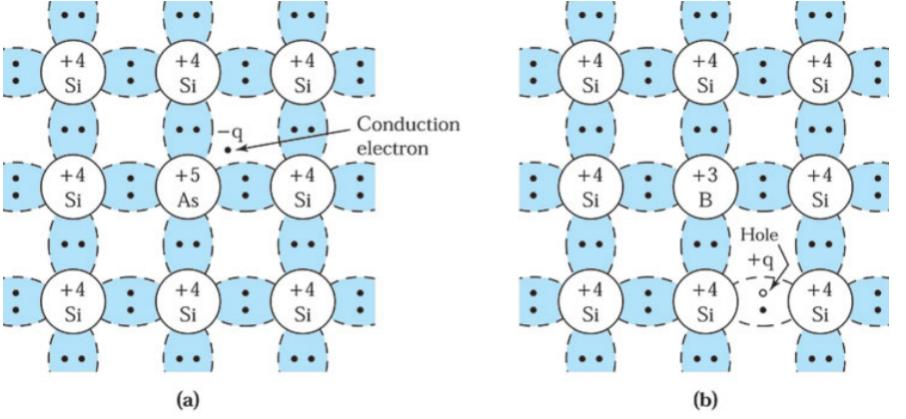
\includegraphics[width=12cm]{figures/ch01/doping.jpg}
\caption{Doping with (a) donor atoms and (b) acceptor atoms} 
\label{fig:doping}
\end{figure} 

Conventionnellement, nous utilisons $N_d$ pour la concentration de donneurs et $N_a$ pour la densité d'accepteurs. Ils ont des valeurs typiques de $10^{16}/cm^3$. Cela est beaucoup plus faible que le nombre d'atomes ($\sim 10^{20}/cm^3$), mais beaucoup plus élevé que la concentration intrinsèque de porteurs $n_i$ ($\sim 10^{10}/cm^3$). Nous parlerons de semi-conducteurs de type n ou p lorsque nous parlons de dopage avec des donneurs ou des accepteurs, respectivement.\\
L'expression \ref{eq:carrier_density2} reste valable, également dans un semi-conducteur dopé. Par conséquent, les porteurs de charge majoritaires (électrons dans un semi-conducteur de type n, trous dans un semi-conducteur de type p) sont largement plus nombreux que les porteurs de charge minoritaires (trous dans un semi-conducteur de type n, électrons dans un semi-conducteur de type p). Dans le cas d'un semi-conducteur de type n, par exemple, nous supposons que tous les atomes donneurs perdent leur électron supplémentaire et deviennent ionisés. Ainsi, $n_n = N_d \approx 10^{16}/cm^3$. En conséquence, $p_n = n_i^2/n_n \approx 10^{4}/cm^3$. Notez le sous-script $n$ pour indiquer qu'il s'agit d'un semi-conducteur de type n.\\
Le niveau de Fermi pour les semi-conducteurs dopés (ou \emph{extrinsèques}) ne se situe plus à mi-chemin entre la bande de valence et la bande de conduction. Puisque:
$$
n_n = N_d =  N_C e^{-(E_C-E_{Fn})/kT}\Rightarrow E_{Fn} = E_C - kT \ln \frac{N_d}{N_C} \\
$$
et nous savons également que $E_{i} = E_C - kT \ln \frac{n_i}{N_C}$ pour un semi-conducteur intrinsèque. Ainsi:
$$
E_{Fn} = E_{i} + kT \ln \frac{N_d}{n_i}
$$
and 
$$
E_{Fp} = E_{i} - kT \ln \frac{N_a}{n_i}
$$
Cela signifie que dans un semi-conducteur de type n, le niveau de Fermi se situe au-dessus du niveau de Fermi intrinsèque, tandis que dans un semi-conducteur de type p, il se situe en dessous. De plus, le niveau de Fermi se rapproche de la bande de conduction (de valence) si $N_d$ ($N_a$) est plus élevé. La figure \ref{fig:doping2} montre comment la distribution de charges change dans un semi-conducteur de type n, en raison d'un déplacement du niveau de Fermi $E_{Fn}$. Notez également le surplus d'électrons par rapport aux trous, puisque presque tous les électrons de la bande de conduction proviennent de l'ionisation des atomes donneurs.
\begin{figure}[h!]
\centering
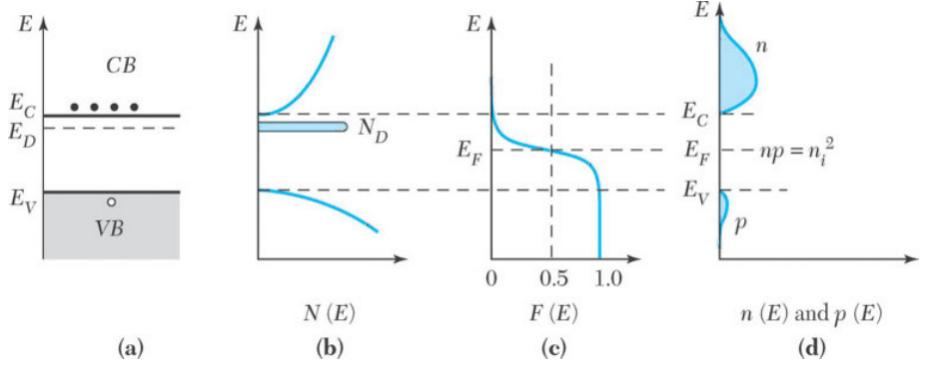
\includegraphics[width=13cm]{figures/ch01/doping2.jpg}
\caption{Carrier density due to donor doping in n-type semiconductor} 
\label{fig:doping2}
\end{figure}


Si nous transformons les énergies en potentiels via la relation $E = -q V$ et définissons $V$ comme la différence de potentiel entre le niveau de Fermi intrinsèque et réel : $V = V_{Fi} - V_F$, nous pouvons réécrire ces équations et obtenir les \emph{équations de Boltzmann}:
\begin{equation} 
\begin{split}
n &= n_i \; e^{qV/kT}  = n_i e^{V/v_{th}}  \\
p &= n_i \; e^{-qV/kT} = n_i e^{-V/v_{th}}
\label{eq:boltzamnn_eqns}
\end{split}
\end{equation}
avec $v_{th} = kT/q$ la tension thermique ($\approx 26$ mV à $T=300$ K). Ces équations ne sont valables qu'à l'équilibre thermique, c'est-à-dire lorsqu'il n'y a pas d'écoulement de charges.

\subsection{Transport de Porteurs}
Plusieurs mécanismes de transport de porteurs existent dans un semi-conducteur. Nous discutons ici les deux plus courants : le courant de dérive, dû à la présence d'un champ électrique, et le courant de diffusion, dû à un gradient de concentration.
\subsection{Courant de Dérive}
En l'absence d'un champ électrique, les charges se déplacent de manière aléatoire en raison de leur énergie thermique. Cependant, puisque le mouvement est aléatoire, il n'existe aucune direction préférentielle de déplacement. Cela change lorsque un champ électrique externe est appliqué. En présence d'un champ électrique $\mathcal{E}$, un électron avec une charge $-q$ est accéléré par une force $F_1 = -q \mathcal{E}$. Cependant, en même temps, la charge interagit avec le réseau cristallin et est ralentie par des collisions avec les atomes et les impuretés. Cette force d'amortissement $F_2$ est proportionnelle à la vitesse de la particule : $F_2 = -\alpha v_d$, avec $\alpha$ le facteur d'amortissement. Ainsi :
$$
m_e^* \frac{d v_d}{dt}  = -q \mathcal{E}  - \alpha v_d
$$
La particule atteindra une vitesse d'équilibre $v_{d0}$ lorsque $\frac{d v_d}{dt} = 0$, ainsi $v_{d0} = \frac{-qE}{\alpha}$. Nous pouvons résoudre l'équation du premier ordre pour une particule qui est initialement à une vitesse $v_d(0) = 0$ et obtenir $v_d(t) = v_{d0} e^{-t/ \tau_e}$ où $ \tau_e = \frac{m_e^*}{\alpha}$ est un temps caractéristique appelé \emph{temps de relaxation}. Il est proportionnel au temps nécessaire pour atteindre $v_{d0}$ et est de l'ordre de $1$ ps.\
D'un point de vue macroscopique, pour calculer le courant électronique total, nous devons faire la moyenne sur tous les électrons disponibles pour la conduction, c'est-à-dire les électrons présents dans la bande de conduction. Après quelques calculs, nous obtenons pour la densité de courant électronique $J_n = q \mu_n n \mathcal{E}$ avec la \emph{mobilité des électrons} $\mu_n = \frac{q \tau_e}{m_e^*}$. Une expression similaire peut être trouvée pour la densité de courant de trous $J_p$. Le courant total est la somme des deux:
\begin{equation}
    J = J_n + J_p = q(\mu_n n + \mu_p p) \mathcal{E} = \sigma \mathcal{E}
\end{equation}
Ceci est la formulation de la loi d'Ohm pour un semi-conducteur.
\subsection{Structure de bande sous polarisation}
Nous considérons la conduction dans un matériau semi-conducteur homogène due à un champ électrique. La figure \ref{fig:bandbiasing} montre un semi-conducteur de type n et son diagramme de bande à l'équilibre thermique (à gauche) et le diagramme de bande lorsqu'une tension de polarisation positive est appliquée à la borne de droite (à droite). Lorsqu'un champ électrique E est appliqué à un semi-conducteur, chaque électron subit une force $-q \mathcal{E}$ du champ. La force est égale au gradient négatif de l'énergie potentielle :
$$
-q \mathcal{E} = \frac{dE_C}{dx}
$$
Puisque nous nous intéressons au gradient de l'énergie potentielle, nous pouvons utiliser n'importe quelle partie du diagramme de bande qui est parallèle à $E_C$. Il est pratique d'utiliser le niveau de Fermi intrinsèque $E_{i}$ car nous l'utiliserons lorsque nous considérerons les jonctions p-n. Ainsi:
$$
\mathcal{E} = -\frac{1}{q}\frac{dE_C}{dx} = -\frac{1}{q}\frac{dE_i}{dx} 
$$
Nous pouvons définir une quantité associée $V$ comme le potentiel électrostatique dont le gradient négatif est égal au champ électrique: $\mathcal{E} = - \frac{d V}{dx}$. En comparant les deux équations, nous obtenons $V = -\frac{E_i}{q}$, ce qui établit une relation entre le potentiel électrostatique et l'énergie potentielle d'un électron. Pour le semi-conducteur homogène illustré à la figure \ref{fig:bandbiasing}, l'énergie potentielle et $E_i$ diminuent linéairement avec la distance ; ainsi, le champ électrique est constant dans la direction négative de x. Sa magnitude est la tension appliquée divisée par la longueur de l'échantillon.\\
\begin{figure}[h!]
\centering
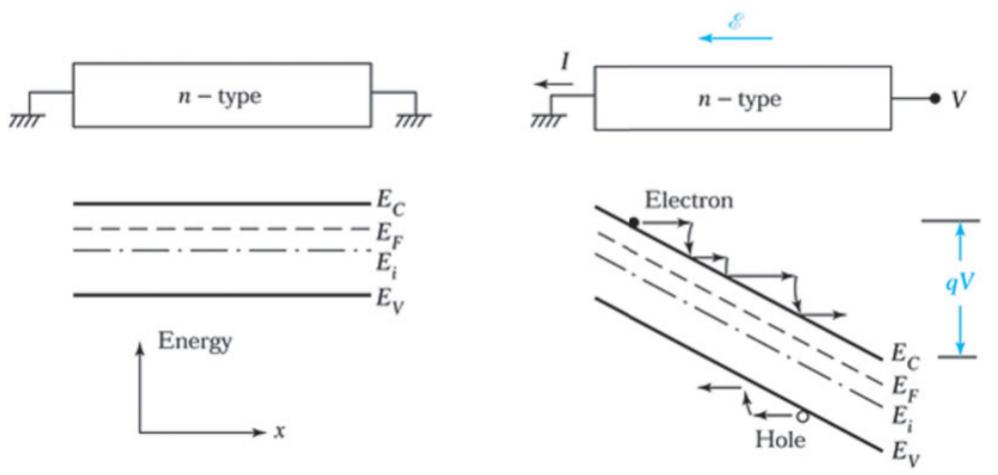
\includegraphics[width=12cm]{figures/ch01/bandbiasing.jpg}
\caption{Band structure under biasing} 
\label{fig:bandbiasing}
\end{figure}
Les électrons de la bande de conduction se déplacent vers le côté droit. L'énergie cinétique correspond à la distance par rapport au bord de bande (c'est-à-dire $E_C$ pour les électrons). Lorsqu'un électron subit une collision, il perd une partie ou la totalité de son énergie cinétique vers le réseau cristallin et retourne à sa position d'équilibre thermique. C'est l'origine du facteur d'atténuation $\alpha$ de la section précédente. Après que l'électron a perdu une partie ou la totalité de son énergie cinétique, il commencera à nouveau à se déplacer vers la droite et le même processus se répétera plusieurs fois. La conduction par les trous peut être visualisée de manière similaire mais dans la direction opposée.

\subsection{Courant de diffusion}
Un autre mécanisme de transport est la diffusion où les porteurs se déplacent d'un endroit à un autre en raison de la variation spatiale de la concentration de porteurs. Comme les porteurs se déplacent au hasard en raison de l'agitation thermique, plus de porteurs se déplaceront de la concentration de porteurs plus élevée vers celle de porteurs plus faible que dans l'autre sens, entraînant efficacement un mouvement net d'électrons de gauche à droite comme dans la figure \ref{fig:diffusion}. Ce courant est décrit par une équation de diffusion standard :
$$
J_n = q D_n \frac{dn}{dx}
$$
avec $D_p$ le coefficient de diffusion des trous. Une relation equivalente existe pour les trous:
$$
J_p = -q D_p \frac{dp}{dx}
$$
\begin{figure}[h!]
\centering
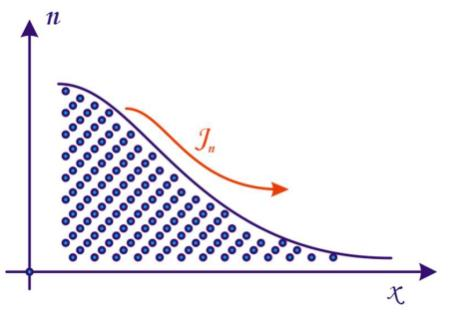
\includegraphics[width=8cm]{figures/ch01/diffusion.jpg}
\caption{Courant $J_n$ dû à la diffusion} 
\label{fig:diffusion}
\end{figure}
Cependant, ce déplacement de porteurs induira un champ électrique $\mathcal{E}$ et donc également un courant de dérive $J = q \mu_n n \mathcal{E}$. Après un certain temps, les deux courants seront égaux et opposés et un équilibre dynamique sera atteint :
$$
J_n = q \mu_n n \mathcal{E} +  q D_n \frac{dn}{dx} = 0
$$
En utilisant les équations de Boltzmann (\ref{eq:boltzamnn_eqns}), on peut déduire une relation entre $D_n$ et $\mu_n$ :
$$
D_n = \frac{kT}{q} \mu_n
$$
et
$$
D_p = \frac{kT}{q} \mu_p
$$
Ces relations sont connues sous le nom d'équations d'Einstein.
\section{Génération et Recombinaison}
\label{sec:generationrecombination}
En équilibre thermique, la relation $pn=n_i^2$ est valide. Il s'agit d'un équilibre dynamique : la génération thermique de paires électron-trou à un taux $G_{th}$ est contrebalancée par les électrons qui retombent de la bande de conduction à la bande de valence (c'est-à-dire un électron libre qui se combine avec un trou pour former une liaison covalente). Ce processus s'appelle la recombinaison.\\
Si des porteurs en excès sont introduits, nous ne sommes plus en équilibre et $pn>n_i^2$. La création de porteurs en excès est appelée \emph{injection de porteurs} et peut être réalisée par excitation optique ou en polarisant directement une jonction pn (voir le chapitre \ref{ch:pnjunction}). Le mécanisme qui rétablit l'équilibre est la recombinaison des porteurs minoritaires injectés avec les porteurs majoritaires présents dans le semi-conducteur. La génération et la recombinaison de porteurs thermiques et en excès sont représentées dans la figure \ref{fig:generationrecombination}.
\begin{figure}[h!]
\centering
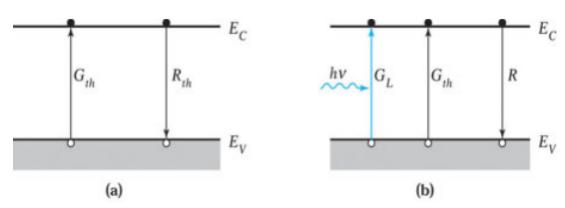
\includegraphics[width=12cm]{figures/ch01/recombination.jpg}
\caption{Generation and recombination under (a) equilibrium and (b) optical excitation} 
\label{fig:recombination}
\end{figure}
Nous supposons que les porteurs en excès conduisent à une recombinaison à une vitesse $R(n, p, T)$. À l'équilibre, $G_{th}(n_0, p_0, T) = R(n_0, p_0, T) = R_{th}$. Lorsque nous créons des porteurs en excès, nous pouvons écrire que $n = n_0 + \delta n$ et $p = p_0 + \delta p$, et nous supposerons que l'injection est faible par rapport aux conditions d'équilibre. Cela signifie que $\delta n \ll n_0$ et $\delta p \ll p_0$. Dans ces conditions, nous pouvons approximer la vitesse de recombinaison par les termes du premier ordre:
\begin{equation} 
\begin{split}
R(n, p, T) &= R(n_0, p_0, T) + (n-n_0) \frac{\partial R}{\partial n} + (p-p_0) \frac{\partial R}{\partial p} \\
           &= G_{th} +  \frac{(n-n_0)}{\tau_n} + \frac{(p-p_0)}{\tau_p} 
\end{split}
\end{equation} 
Dans un matériau de type n, le taux de recombinaison est déterminé par les trous en excès - car les trous sont beaucoup plus susceptibles de trouver un candidat pour la recombinaison (c'est-à-dire un électron) - que par les électrons en excès. Le taux auquel les porteurs recombinent est donc déterminé par le nombre de porteurs minoritaires :
\begin{itemize}
	\item En type n : $R - G_{th} = \frac{(p-p_0)}{\tau_p}$
	\item En type p : $R - G_{th} = \frac{(n-n_0)}{\tau_n}$
\end{itemize}
La durée de vie des porteurs minoritaires en excès $\tau_p$ et $\tau_n$ est beaucoup plus grande que le temps de relaxation $\tau_e$.
\section{Les équations de continuité}
Le changement de densité de porteurs dans un volume $V$ à l'intérieur d'un semi-conducteur peut être dû à trois causes :
\begin{enumerate}
	\item génération de porteurs,
	\item recombinaison,
	\item flux de porteurs entrant ou sortant du volume à travers la surface environnante $S$
\end{enumerate}
Supposons que nous voulons étudier le changement de la densité d'électrons dans un matériau de type p. Nous pouvons écrire:
\begin{equation} 
	\begin{split}
		-q \iiint_V \frac{\partial n}{\partial t} \; dV &= -q \iiint_V (G-R) \; dV - \varoiint_S \vec{J_n} \vec{n} \; dS \\
		 &= -q \iiint_V (G-R) \; dV - \iiint_V \nabla \vec{J_n}  \; dV \\
	\end{split}
\end{equation} 
où nous avons utilisé le théorème de la divergence. Comme cela est valable pour n'importe quel volume, les termes dans les intégrales doivent être égaux:
\begin{equation} 
	\begin{split}
		-q \frac{\partial n}{\partial t} &= -q (G-R) - \nabla \vec{J_n}\\
										 &= -q (G_{th} + g - R) - \nabla \vec{J_n}\\
	\Rightarrow	\frac{\partial n}{\partial t}	 &= \Big(\frac{n-n_0}{\tau_n}\Big) + \frac{1}{q}\nabla \vec{J_n} + g\\
	\end{split}
\end{equation}
où nous remplaçons $G_{th} - R$ par $\frac{(n-n_0)}{\tau_n}$ puisque nous sommes dans un matériau de type p. En une dimension, cela devient :
\begin{equation} 
	\begin{split}
		\frac{\partial n}{\partial t}	 &= \Big(\frac{n-n_0}{\tau_n}\Big) + \frac{1}{q} \frac{\partial J_n}{\partial x} + g\\
	\end{split}
\label{eq:continuity1}
\end{equation}
où $J_n$ a en général une contribution de dérive et de diffusion : $J_n = q \mu_n n \mathcal{E} + q D_n \frac{dn}{dx}$. En substituant cela dans \ref{eq:continuity1} - avec à la fois $n$ et $\mathcal{E}$ dépendant de $x$ - nous obtenons:
\begin{equation} 
	\begin{split}
		\frac{\partial n}{\partial t}	 &= \Big(\frac{n-n_0}{\tau_n}\Big) - n \mu_n \frac{\partial \mathcal{E}}{\partial x} + \mu_n \mathcal{E} \frac{\partial n}{\partial x} + D_n \frac{\partial^2 n}{\partial x^2} + g\\
	\end{split}
	\label{eq:continuity}
\end{equation}

Cette équation est appelée l'\emph{équation de continuité} pour les porteurs de type n dans un matériau de type p. Des expressions similaires peuvent être trouvées pour les autres cas.

%\begin{equation} 
%\begin{split}
%\frac{\partial n_p}{\partial t} &= n_p \mu_n \frac{\partial \mathcal{E}}{\partial x} + \mu_n \mathcal{E} \frac{\partial n_p}{\partial x} + D_n \frac{\partial^2 n_p}{\partial x^2} + G_{th} - \frac{n_p-n_{p0}}{\tau_n}\\
%\frac{\partial p_n}{\partial t} &= p_n \mu_p \frac{\partial \mathcal{E}}{\partial x} + \mu_p \mathcal{E} \frac{\partial p_n}{\partial x} + D_p \frac{\partial^2 p_n}{\partial x^2} + G_{th} - \frac{p_n-p_{n0}}{\tau_p}\\
%\end{split}
%\label{eq:continuity}
%\end{equation} 
\chapter{La jonction pn}
\label{ch:pnjunction}

%\section{Aperçu du chapitre}
Dans cette section, nous démontrons qu'une jonction formée entre un échantillon de semi-conducteur de type $p$ et un échantillon de type $n$ possède les propriétés d'un redresseur. Ce dispositif à deux bornes est appelé \emph{diode à jonction}. La structure physique et le symbole d'une jonction pn sont présentés dans la figure \ref{fig:pnjunction}.

\begin{figure}[h!]
\centering
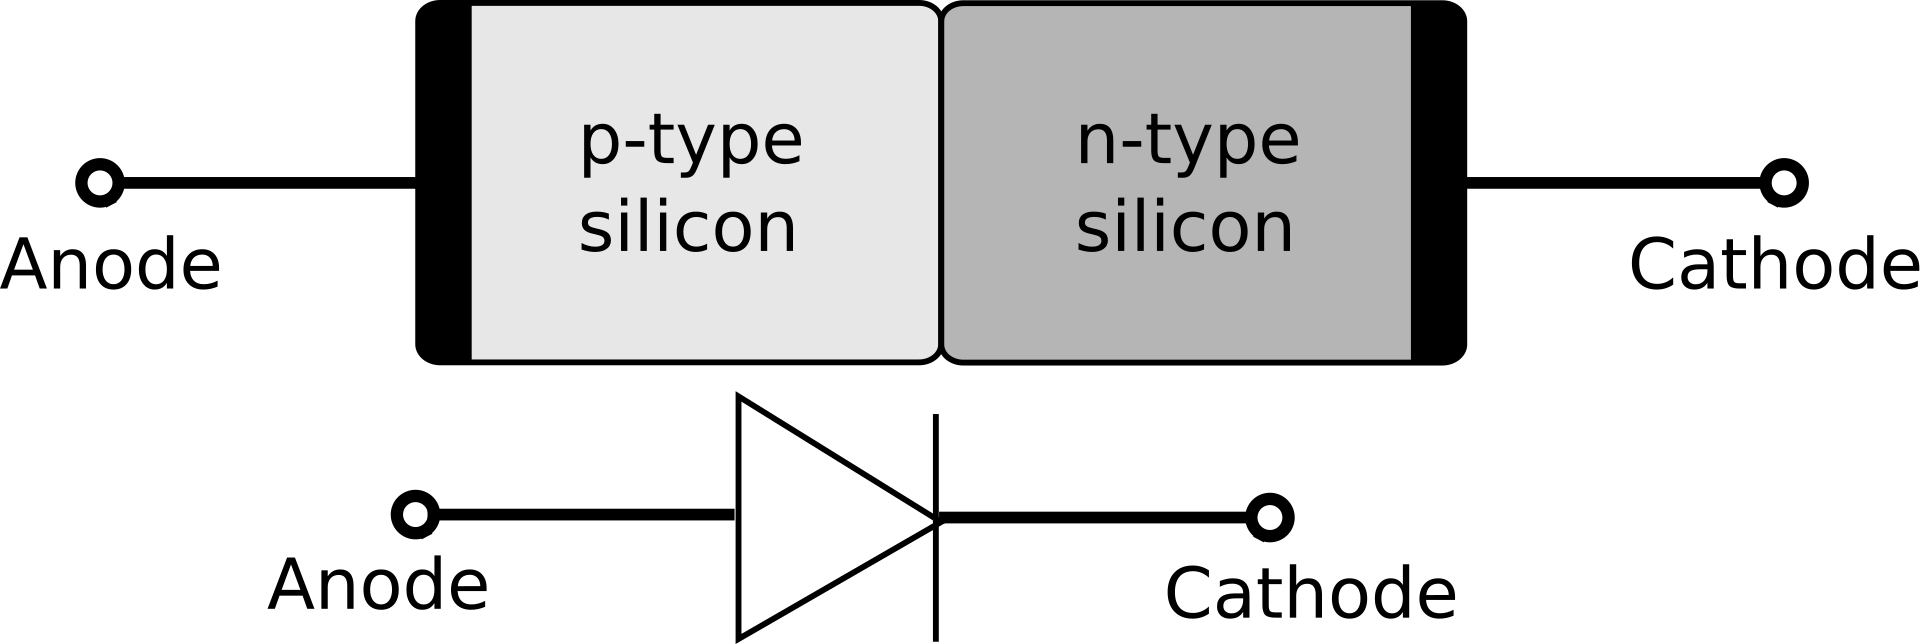
\includegraphics[width=12cm]{figures/ch01/pnjunction.png}
\caption{Structure (above) and symbol (below) of a pn-junction} 
\label{fig:pnjunction}
\end{figure}

Nous discuterons de la jonction en équilibre ainsi que sous polarisation directe et inverse. La caractéristique I-V sera dérivée et les concepts de la rupture de avalanche et de la capacité de déplétion seront abordés.

\section{La jonction pn en équilibre}
Si des impuretés donneuses sont introduites d'un côté et des accepteurs de l'autre côté d'un monocristal d'un semi-conducteur, une jonction $pn$ est formée\footnote{Ceci est appelé une jonction abrupte}. À l'interface, il y a par construction un gradient de concentration et donc des électrons et des trous diffuseront de chaque côté. Les électrons du type n se recombinent avec les trous majoritaires du type p et les trous du type p se recombinent avec les électrons majoritaires du type n. En conséquence, les ions dopants seront exposés et le côté n aura une densité de charge positive fixe ($N_d$) tandis que le côté p aura une densité de charge négative fixe ($N_a$) (figure \ref{fig:pn_equilibrium} (a)). Cette accumulation de charge entraînera un champ électrique interne pointant du type n vers le type p et agira donc contre tout courant de diffusion supplémentaire (\ref{fig:pn_equilibrium} (b)). Nous supposons pour le moment qu'aucune polarisation externe n'est appliquée, de sorte qu'aucun courant net ne peut circuler. La zone où les porteurs majoritaires ont diffusé et se sont recombinés est la \emph{zone de charge d'espace}\footnote{Également appelée la région de déplétion}. Pour préserver la neutralité de charge, nous exigeons que :
$$
N_A \; x_p = N_d \; x_n
$$
avec $x_p$ et $x_n$ la profondeur de la zone de charge d'espace dans le type p et n ($W_{Dp}$ et $W_{Dn}$ dans la figure \ref{fig:pn_equilibrium}). Comme on peut le déduire de cette expression, la zone de charge d'espace s'étend davantage dans le matériau faiblement dopé.\
Parce que $\frac{d\mathcal{E}}{dx} = \rho/\epsilon$, le champ électrique qui résulte de cette accumulation de charge est calculé comme $\mathcal{E}(x) = \int \rho(x)/\epsilon ; dx$ avec $\rho(x)$ le profil de charge local :
\begin{equation}
	\begin{split}
		\rho(x) &= -N_a \text{ si } x < 0 \\
		&= ; N_d \text{ si } x > 0
	\end{split}
\end{equation}
Le champ électrique maximum correspond à l'accumulation de charge totale et est négatif puisque le type p est placé à gauche : $|\mathcal{E}_m| = \epsilon N_a x_p = \epsilon N_d x_n$. Un champ électrique donne naissance à une différence de potentiel puisque $\mathcal{E} = -\frac{d\psi}{dx}$ comme dans la figure \ref{fig:pn_equilibrium}(c) où le soi-disant potentiel de jonction $\psi{bi}$ est égal à la surface sous $\mathcal{E}(x)$:
$$
\psi_{bi} = \frac{1}{2} (x_n + x_p) |\mathcal{E}_m| = \frac{1}{2} \epsilon (x_n + x_p)  N_a x_p
$$
Cette tension de jonction est également visible sur la figure \ref{fig:pn_equilibrium} (d) où les bandes d'énergie sont représentées. En raison du champ électrique, les bandes se courbent (dans la direction opposée à celle du potentiel, car $E=-qV$) à la jonction. Cette dernière figure est importante et peut également être construite en raisonnant avec les niveaux de Fermi. \
La largeur totale $W = x_n + x_p$ de la région de charge d'espace peut être calculée en fonction des niveaux de dopage et de la tension de jonction intrinsèque. Le résultat est :
\begin{equation}
    W = \sqrt{\frac{2 \epsilon}{q} \Big(\frac{N_a + N_d}{N_a N_d}\Big) V_{bi}}
    \label{eq:SCR_width}
\end{equation}

\begin{figure}[h!]
	\centering
	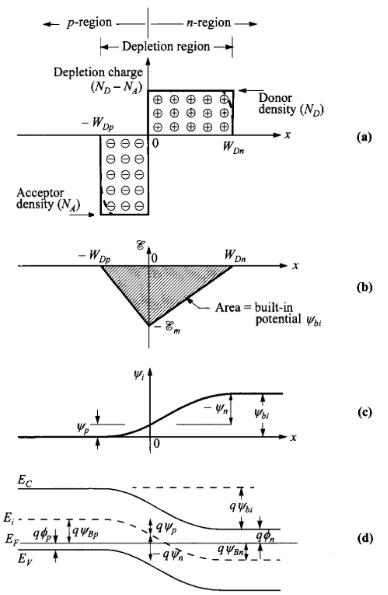
\includegraphics[width=8cm]{figures/ch01/pn_equilibrium.jpg}
	\caption{jonction pn en équilibre thermique}
	\label{fig:pn_equilibrium}
\end{figure}
\subsection{Niveaux de Fermi en équilibre}
Puisqu'aucun courant net ne peut circuler dans la jonction sans polarisation externe, le courant de dérive doit être égal au courant de diffusion. Pour les trous, cette condition donne:
\begin{equation}
    \begin{split}
       J_p  &= J_{p, drift} + J_{p, diffusion} \\
            &= q \mu_p p \mathcal{E} - q D_p \frac{dp}{dx} \\
            &= q \mu_p p \Big(\frac{1}{q} \frac{dE_i}{dx} \Big) - k T \mu_p \frac{dp}{dx}  = 0\\
    \end{split}
    \label{eq:jp_equilibrium}
\end{equation}
En équilibre, nous pouvons appliquer les équations de Boltzmann :
\begin{equation}
    p = n_i e^{(E_i - E_F)/kT}
    \label{eq:boltzmann_ch2}
\end{equation}
et calculer $\frac{dp}{dx}$ :
$$
\frac{dp}{dx} = \frac{p}{kT} \Big( \frac{dE_i}{dx} - \frac{dE_F}{dx} \Big)
$$
En substituant ceci dans l'équation \ref{eq:jp_equilibrium}, nous obtenons :
$$
J_p = \mu_p p \frac{dE_F}{dx} = 0 
$$
ou $\frac{dE_F}{dx} = 0$. Un résultat similaire est valable pour les électrons. \textbf{Pour qu'il y ait zéro courant net d'électrons et de trous, le niveau de Fermi doit être constant.}\\
Comme on peut le voir dans la figure \ref{fig:pn_equilibrium}(d), le niveau de Fermi $E_F$ reste constant le long de la jonction car il n'y a pas de courant net. Étant donné que $E_F$ est proche de $E_V$ dans le matériau de type p et proche de $E_C$ dans le matériau de type n, les bandes doivent se plier comme dans la figure pour maintenir un $E_F$ constant.

\subsection{Le potentiel de jonction intrinsèque}
Nous allons maintenant calculer $V_{bi} = \psi_n - \psi_p$ (précédemment noté $\psi_{bi}$). Nous savons qu'à distance de la jonction, il n'y a pas de charges nettes présentes, donc le potentiel doit obéir à l'équation de Laplace:
$$
\frac{d^2 \psi}{dx^2} = 0
$$
et $N_d - N_a + p - n = 0$ pour préserver la neutralité de charge. Dans un matériau de type p, nous supposons que $N_d = 0$ et $p \gg n$. Cela donne $p = N_a$. En insérant cela dans l'équation \ref{eq:boltzmann_ch2}, on obtient :
$$
\psi_p = -\frac{1}{q} (E_i - E_f) |_{x < x_p} = \frac{kT}{q} \ln\Big(\frac{N_a}{n_i}\Big)
$$
De même, le potentiel électrostatique pour le matériau de type n est
$$
\psi_n = -\frac{1}{q} (E_i - E_f) |_{x > x_n} = \frac{kT}{q} \ln\Big(\frac{N_d}{n_i}\Big)
$$
Le potentiel de jonction intrinsèque $V_{bi}$ est la différence de potentiel électrostatique entre le côté p et le côté n à l'équilibre thermique:
\begin{equation}
    V_{bi} = \psi_n - \psi_p = \frac{kT}{q} \ln\Big(\frac{N_a N_d}{n_i^2}\Big)
    \label{eq:vbi}
\end{equation}

\section{La jonction pn sous polarisation.}

\subsection{Polarisation directe}
Supposons que nous appliquons une tension positive $V_F$ à l'anode (côté p) tout en maintenant la cathode (côté n) à la masse. L'effet est que nous réduisons la barrière du potentiel intégré de $V_{bi}$ à $V_{bi}-V_F$, comme illustré sur le côté gauche de la figure \ref{fig:pn_bias}. Cela a plusieurs conséquences :
\begin{itemize}
	\item La largeur de la région de déplétion va diminuer, car l'équation \ref{eq:SCR_width} peut être réécrite comme :
	\begin{equation}
		W = \sqrt{\frac{2 \epsilon}{q} \frac{N_a + N_d}{N_a N_d} (V_{bi} - V_F)}
		\label{eq:SCR_width_bias}
	\end{equation}
	\item La valeur maximale de la $\mathcal{E}$  est réduite. Cela signifie qu'il y a un déséquilibre entre le courant de diffusion et le courant de dérive, et qu'il y aura un flux net (de diffusion) de trous du côté p vers le côté n et un flux d'électrons du côté n vers le côté p. Le résultat est un courant net du côté p vers le côté n.\footnote{Remarquez que les électrons peuvent diffuser de basse à haute énergie, alors qu'ils dérivent toujours de haute à basse énergie.}
\end{itemize}
Il y a donc un courant de diffusion de porteurs majoritaires à travers la région de déplétion vers l'autre côté, où ils deviennent les porteurs minoritaires. Comme il y a beaucoup de porteurs majoritaires disponibles, ce courant peut devenir très important lorsque la barrière de potentiel est suffisamment abaissée.\\
Remarquez également que les niveaux de Fermi dans la figure \ref{fig:pn_bias} ne sont plus constants, car il y a un courant et nous ne sommes plus en équilibre.

\begin{figure}[h!]
\centering
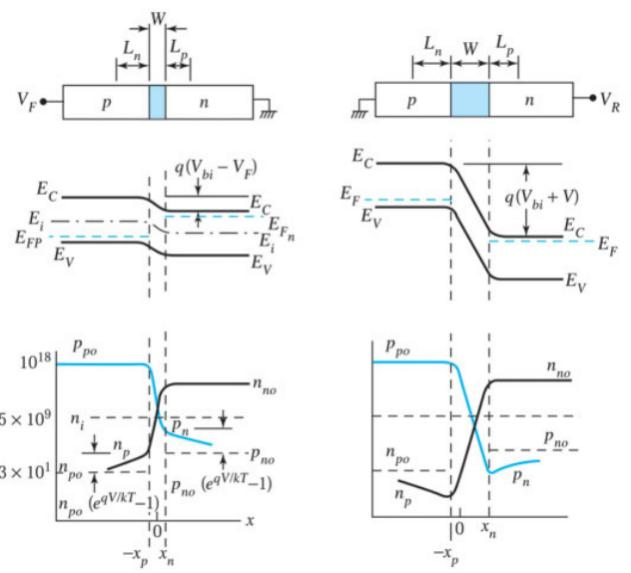
\includegraphics[width=12cm]{figures/ch01/pn_bias.jpg}
\caption{pn-junction under forward (left) and reverse (right) bias} 
\label{fig:pn_bias}
\end{figure}

\subsection{Polarisation inverse}
Lorsque nous appliquons une tension positive $V_R$ à la cathode (côté n) tout en gardant l'anode à la masse, nous augmentons la barrière du potentiel intégré à $V_{bi}+V_R$. Cette situation est esquissée à droite de la figure \ref{fig:pn_bias}. Selon l'équation \ref{eq:SCR_width_bias}, la largeur de la région de charge d'espace augmentera (parce que nous pouvons remplacer $V_F$ par $-V_R$). Le champ électrique interne au niveau de la jonction devient plus grand qu'avant, donc il peut y avoir un courant de dérive net. Cependant, les porteurs disponibles pour être balayés à travers la région de charge d'espace par le champ électrique sont les porteurs minoritaires des deux côtés de la jonction. Par conséquent, le courant résultant (le courant de saturation) sera très faible.

\subsection{Caractéristique de la diode}
Calculons les courants en supposant :
\begin{enumerate}
	\item que la région de déplétion a des limites abruptes et que, en dehors de ces limites, le semi-conducteur est supposé neutre ;
	\item que les densités de porteurs aux limites sont liées par la différence de potentiel électrostatique à travers la jonction ;
	\item que les densités de porteurs minoritaires injectés sont petites par rapport aux densités de porteurs majoritaires ;
	\item qu'il n'y a ni courant de génération ni courant de recombinaison dans la région de déplétion et que les courants d'électrons et de trous sont constants dans toute la région de déplétion.
\end{enumerate}
À l'équilibre, nous avons $p_{p0} = N_a$ et $n_{n0} = N_d$. En utilisant la loi de masse-action $p_{p0} ; n_{n0} = n_i^2$, nous pouvons réécrire l'équation \ref{eq:vbi} comme suit :
$$
V_{bi} = \frac{kT}{q} \ln \frac{p_{p0} n_{n0}}{n_i^2} = \frac{kT}{q} \ln \frac{n_{n0}}{n_{p0}}
$$
En réarrangeant cela, on obtient :
\begin{equation}
    \begin{split}
        n_{n0} &= n_{p0} e^{qV_{bi}/kT}
    \end{split}
    \label{eq:nn0}
\end{equation}
et
\begin{equation}
	\begin{split}
		p_{p0} &= p_{n0} e^{qV_{bi}/kT}
	\end{split}
	\label{eq:pp0}
\end{equation}
En raison de la deuxième hypothèse, ces équations restent valables lorsque nous changeons le potentiel net. Ainsi :
\begin{equation}
    \begin{split}
        n_{n} &= n_{p} e^{q(V_{bi}-V_F)/kT}
    \end{split}
    \label{eq:nn}
\end{equation}
avec $n_n$ et $n_p$ les densités d'électrons hors équilibre aux limites de la région de charge d'espace aux côtés n et p, respectivement. En substituant \ref{eq:nn0} dans \ref{eq:nn}, on obtient la densité d'électrons à la limite de la région de déplétion du côté p ($x = -x_p$) :
\begin{equation}
	n_p = n_{p0}\;e^{qV/kT}
\end{equation}
et de même :
\begin{equation}
	p_n = p_{n0}\;e^{qV/kT}
	\label{eq:density_junction}
\end{equation}
où $V$ peut être à la fois $V_F$ ou $V_R$, c'est-à-dire la tension appliquée à travers la jonction depuis l'extérieur. On peut également écrire cela comme:
\begin{equation}
	\begin{split}
		n_p - n_{p0} &= n_{p0}(e^{qV/kT} - 1) \\
		p_n - p_{n0} &= p_{0}(e^{qV/kT} - 1)
	\end{split}
\label{eq:pexcess_depletion}
\end{equation}
Notez que les porteurs minoritaires aux limites de la région de charge d'espace augmentent considérablement au-dessus de leur équilibre en polarisation directe. Ainsi, il y a une injection de porteurs minoritaires dans la région de déplétion.\
Dans la région n neutre, il n'y a pas de champ électrique, donc l'équation de continuité à l'état stationnaire \ref{eq:continuity} se réduit à :

\begin{equation}
	\frac{\partial p_n}{\partial t} = D_p \frac{d^2p}{dx^2} - \frac{p_n - p_{n0}}{\tau_p} = 0
\end{equation}
En résolvant cette équation avec les conditions aux limites de l'équation \ref{eq:pexcess_depletion} et $p_n(x = \infty) = p_{n0}$, on obtient:

\begin{equation}
	p_n - p_{n0} = p_{n0} (e^{qV/kT} - 1) e^{-(x-x_n)/L_p}
\end{equation}
avec $L_p = \sqrt{D_p \tau_p}$ la longueur de diffusion des trous. Ce graphe est représenté dans la partie inférieure gauche de la figure \ref{fig:pn_bias}. À la frontière $x=x_n$ :

\begin{equation}
J_p(x_n) = -qD_p \frac{dp_n}{dx}\Bigg|_{x=x_n} = \frac{qD_pp_{n0}}{L_p}(e^{qV/kT} - 1)
\end{equation} 

En appliquant le même raisonnement pour la région n, nous obtenons une relation similaire pour $J_n$. Comme le courant total est la somme des deux, nous trouvons finalement :
\begin{equation}
	J = J_p(x_n) + J_n(-x_p) = J_S(e^{qV/kT} - 1)
	\label{eq:ideal_diode}
\end{equation}
avec $J_S$ le courant de saturation :
\begin{equation}
	J_S = \frac{qD_n p_{n0}}{L_p} + \frac{D_n n_{p0}}{L_n}
\end{equation}
L'équation \ref{eq:ideal_diode} est l'équation de la diode. Son graphique est montré dans la figure \ref{fig:diode_charac}. Il est important de remarquer que le courant augmente de manière exponentielle lorsque $V>0$ car la barrière de potentiel est enlevée. La jonction agit comme un conducteur. D'autre part, lorsque $V<0$, il y a seulement un petit courant de saturation qui n'est pas impacté par la valeur de $V$. La jonction est un circuit ouvert (avec une perte de courant).

\begin{figure}[h!]
\centering
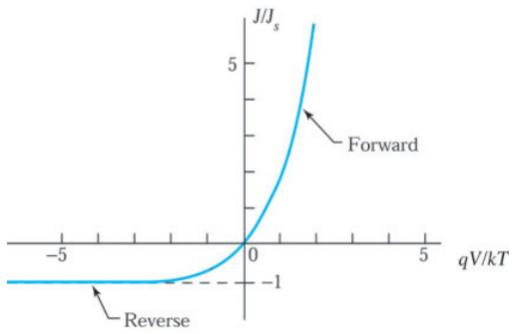
\includegraphics[width=8cm]{figures/ch01/diode_charac.jpg}
\caption{Current characteristic of equation \ref{eq:ideal_diode}}
\label{fig:diode_charac}
\end{figure}

\subsection{Caractéristique pratique de la diode}
L'équation \ref{eq:ideal_diode} donne une densité de courant. En multipliant par la surface $A$ de la section transversale de la jonction, on obtient la courbe I-V:
\begin{equation}
	i_D = I_S(e^{v_D/v_{th}} - 1)
	\label{eq:idiode_IV}
\end{equation}
avec $v_{th} = \frac{kT}{q} \approx 26 mV$ (à $T=300K$) la tension thermique (voir figure \ref{fig:diode_charac2}). Lorsque $v_D \gg v_{th}$:
\begin{equation}
	i_D \approx I_S e^{v_D/v_{th}}
\end{equation}
De plus, lorsque $v_D$ augmente d'environ $60 mV$, le courant $i_D$ est multiplié par un facteur de 10. Comme on peut le voir dans la figure \ref{fig:diode_charac2}, on peut considérer $v_D = 0,6V$ comme une tension de seuil:
\begin{itemize}
	\item Si $v_D > 0,6V$, la diode conduira,
	\item Si $v_D < 0,6V$, la diode ne conduira pas.
\end{itemize}
Ainsi, la diode fonctionne comme un redresseur: seul le courant de la région p vers la région n peut passer, tandis que l'autre direction est bloquée. Bien sûr, en raison du courant de saturation et de l'effet avalanche (voir \ref{sec:avalanche}), cela n'est pas tout à fait vrai.

\begin{figure}[h!]
\centering
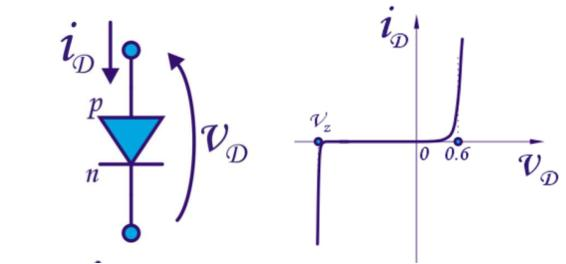
\includegraphics[width=8cm]{figures/ch01/diode_charac2.jpg}
\caption{Symbole et courbe I-V} 
\label{fig:diode_charac2}
\end{figure}

\section{Effet tunnel et avalanche}
\label{sec:avalanche}
Sur la figure \ref{fig:diode_charac2}, on peut voir qu'il y a également un point où la diode va conduire sous polarisation inverse. Ce phénomène peut avoir deux causes: soit il s'agit d'une rupture de la jonction due à l'effet avalanche, soit il s'agit d'une rupture Zener due à l'effet tunnel. La rupture de la jonction se produit à des tensions élevées et est généralement indésirable. La rupture Zener peut être utile et le dopage est adapté de manière à ce qu'elle se produise à quelques volts. Elle est utilisée, par exemple, dans les références de tension (voir le chapitre \ref{ch:references}).\\
\begin{minipage}{.5\textwidth}
	\centering
	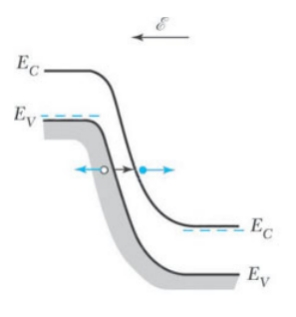
\includegraphics[height=6cm]{figures/ch01/tunnel_effect.jpg}
	\captionof{figure}{}
	\label{fig:tunnel_effect}
\end{minipage}
\begin{minipage}{.5\textwidth}
	\centering
	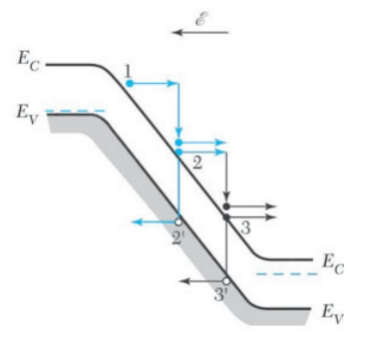
\includegraphics[width=6cm]{figures/ch01/avalanche.jpg}
	\captionof{figure}{}
	\label{fig:avalanche}
\end{minipage}\\
L'\emph{effet tunnel} repose sur la diffusion quantique : lorsque un champ électrique élevé est appliqué à une jonction p-n dans la direction inverse, comme dans la figure \ref{fig:tunnel_effect}, la distance entre la bande de valence et la bande de conduction devient localement très étroite. Dans ces circonstances, un électron de valence peut effectuer une transition de la bande de valence à la bande de conduction. Ce processus, au cours duquel un électron pénètre dans la bande interdite d'énergie, est appelé effet tunnel. L'électron et le trou résultants sont ensuite balayés par le champ électrique à travers la région de charge d'espace, ce qui crée un courant de Zener.

On parle d'\emph{effet avalanche} lorsqu'un électron généré thermiquement dans la région de charge d'espace (désignée par $1$ dans la figure \ref{fig:avalanche}) acquiert de l'énergie cinétique du champ électrique. Si le champ est suffisamment élevé, l'électron peut acquérir suffisamment d'énergie cinétique pour, lors d'une collision avec un atome, briser les liaisons du réseau, créant une paire électron-trou ($2$ et $2'$). L'électron et le trou nouvellement créés acquièrent tous deux de l'énergie cinétique du champ et créent des paires électron-trou supplémentaires (par exemple, $3$ et $3'$). Ce processus se poursuit, créant d'autres paires électron-trou. On appelle donc cette multiplication d'avalanche.

\section{Capacité de déplétion}
\label{sec:depletion_capacitance}

Lorsque nous polarisons en inverse une jonction pn, des charges positives supplémentaires apparaissent du côté n et des charges négatives supplémentaires du côté p. Ainsi, le dispositif fonctionne essentiellement comme un \emph{condensateur}. En substance, nous pouvons considérer les sections conductrices $n$ et $p$ comme les deux plaques du condensateur. Nous supposons également que la charge dans la région de déplétion réside de manière équivalente sur chaque plaque.\\
Mais ce n'est pas tout : à mesure que $V_R$ augmente, la largeur de la région de déplétion augmente également. Autrement dit, la capacité de la structure diminue à mesure que les deux plaques s'éloignent l'une de l'autre. La jonction affiche donc une capacité dépendante de la tension. Nous pouvons montrer que la capacité de la jonction $C_j$ est donnée par :
\begin{equation}
	C_j = \frac{C_{j0}}{\sqrt{1 - \frac{V_R}{V_{bi}}}}
\end{equation}
avec $C_{j0}$ la capacité à polarisation nulle ($V_R = 0$).\
Une jonction pn sous polarisation inverse est donc un condensateur contrôlable par la tension. Ce type de dispositif a de nombreuses utilisations, comme par exemple dans les circuits accordables en fréquence.

\section{Photodétecteur}
Lorsque nous polarisons une jonction pn constituée d'un semi-conducteur à bande directe comme le GaAs, nous créons un photodétecteur, comme dans la figure \ref{fig:photodetector}. Si un photon heurte un électron dans une liaison covalente, il peut rompre cette liaison si l'énergie $h \nu$ est supérieure à l'énergie de la bande interdite. La paire électron-trou résultante est ensuite balayée à travers la région de charge d'espace par le champ électrique appliqué. Ils recombinent dans les zones neutres, générant un courant proportionnel au nombre de photons qui heurtent la jonction.

\begin{figure}[h!]
	\centering
	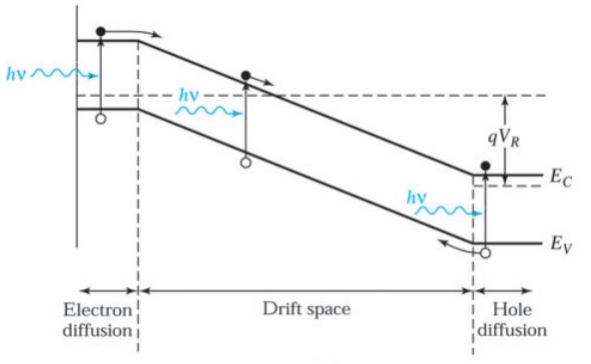
\includegraphics[width=10cm]{figures/ch01/photodetector.jpg}
	\caption{Photodetector operation} 
	\label{fig:photodetector}
\end{figure}

\chapter{Les Transistors}

%\section{Chapter Overview}
Un transistor est un dispositif à semi-conducteur utilisé pour amplifier ou commuter des signaux électriques et de puissance. C'est un composant avec (au moins) trois terminaux. Une tension ou un courant appliqué à l'un des terminaux contrôle le courant à travers une autre paire de terminaux. Comme la puissance contrôlée (sortie) peut être supérieure à la puissance de contrôle (entrée), un transistor peut amplifier un signal.\\
%We will discuss the bipolar junction transistor (BJT) and two transistors based on the field-effect, namely the junction FET and the Metal-Oxide-Semiconductor Field Effect transistor (MOSFET).
Nous discuterons des deux transistors les plus courants : le transistor bipolaire à jonction (BJT) et le transistor à effet de champ à semiconducteur métal-oxyde (MOSFET).

\section{Transistor bipolaire à jonction}
\label{sec:bipolar_junction}
Un transistor bipolaire à jonction (BJT) est formé en plaçant un semi-conducteur de type n entre deux semi-conducteurs de type p (pnp) - ou vice versa (npn), comme le montre la figure \ref{fig:bjt1}. Dans le cas du transistor pnp, la région fortement dopée $p^+$ est appelée l'\emph{émetteur} (E). La région $n$ centrale étroite est la \emph{base} (B). Sa largeur est petite par rapport à la longueur de diffusion des porteurs minoritaires. La région $p$ légèrement dopée est le \emph{collecteur} (C). La figure \ref{fig:bjt1} montre également les symboles de circuit pour les deux transistors BJT, ainsi que les directions conventionnelles pour les tensions et les courants.\
Nous discuterons en détail du transistor pnp ; le raisonnement pour le transistor npn est similaire et sera laissé en exercice.

\begin{figure}[h!]
\centering
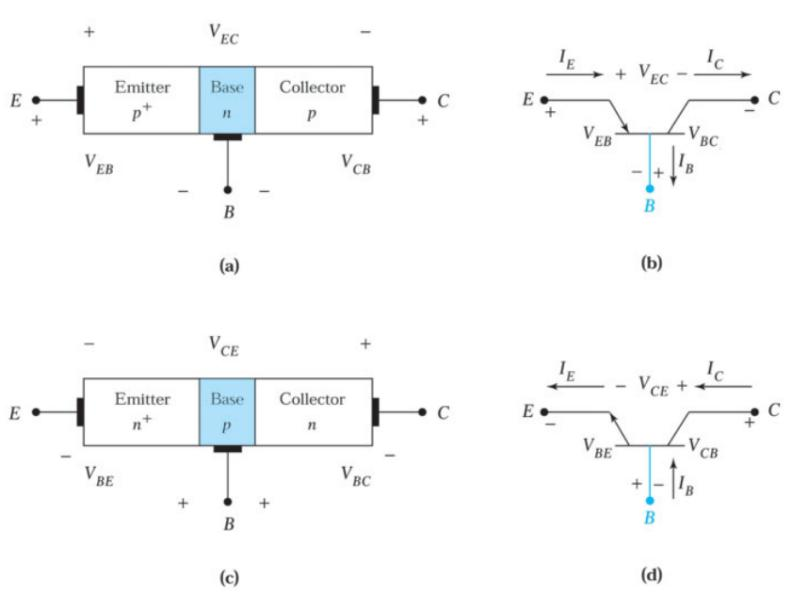
\includegraphics[width=12cm]{figures/ch01/bjt1.jpg}
\caption{(a) Schéma idéalisé unidimensionnel d'un transistor bipolaire p-n-p et (b) son symbole de circuit. (c) Schéma idéalisé unidimensionnel d'un transistor bipolaire n-p-n et (d) son symbole de circuit.} 
\label{fig:bjt1}
\end{figure}

\subsection{Fonctionnement en mode actif}
Considérons d'abord le transistor pnp avec les trois bornes (émetteur, base et collecteur) connectées à la masse comme le montre la figure \ref{fig:bjt2} (a). Dans ces circonstances, nous pouvons construire le profil de charge comme nous l'avons fait pour la jonction pn. Remarquez que les régions de charge d'espace aux deux jonctions s'étendent plus profondément dans les régions moins dopées (base dans la jonction E-B, collecteur dans la jonction B-C).

\begin{figure}[h!]
\centering
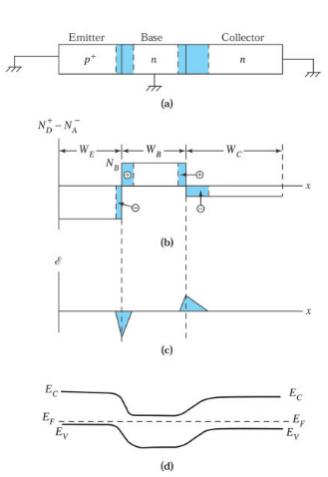
\includegraphics[width=8cm]{figures/ch01/bjt2.jpg}
\caption{(a) pnp transistor with all leads grounded (b) Charge profile in equilibrium (c) Electric field (d) Energy band diagram.} 
\label{fig:bjt2}
\end{figure}
Comme pour la jonction pn, le champ électrique qui apparaît dans la région de charge d'espace est tel qu'il est en équilibre avec le courant de diffusion dû aux gradients de concentration aux jonctions. La figure \ref{fig:bjt2}(d) montre le diagramme de bande en équilibre. Étant donné qu'il n'y a pas de courant, le niveau de Fermi $E_F$ est constant dans les trois régions.\
Nous allons polariser le transistor en mode actif. C'est le mode le plus couramment utilisé en pratique. Nous le faisons en appliquant une tension positive $V_{EB} > 0$ entre l'émetteur et la base, et une tension négative $V_{CB} < 0$ entre le collecteur et la base. La jonction pn entre l'émetteur et la base est ainsi polarisée directement, tandis que la jonction entre le collecteur et la base est polarisée en inverse.\
Puisque nous appliquons une tension positive à l'émetteur et une tension négative au collecteur (tout en gardant la base à la masse ; ceci est une configuration \emph{base commune}), nous abaissons les bandes d'énergie dans l'émetteur et les élevons dans le collecteur (tout comme dans la jonction pn) - voir la figure \ref{fig:bjt3}(d). Par conséquent, la barrière de potentiel entre l'émetteur et la base est abaissée, de sorte que les porteurs majoritaires du côté émetteur (c'est-à-dire les trous) peuvent diffuser à travers la région de charge d'espace jusqu'à la base. Si la base était beaucoup plus grande que la longueur de diffusion, presque tous les trous injectés se recombineraient avec des électrons dans la base et généreraient un courant de base, tout comme dans une jonction pn ordinaire. Cependant, comme la base est petite, la plupart des trous injectés ne se recombinent pas mais diffusent dans la région de charge d'espace entre la base et le collecteur. Là, ils sont balayés par le champ électrique vers le collecteur. En conséquence, la plupart des trous quittant l'émetteur se retrouvent dans le collecteur. Ce phénomène est appelé \emph{action du transistor}. Il est important de réaliser que le courant de collecteur dépend du courant d'émetteur et donc de la hauteur de la barrière émetteur-base et de $V_{EB}$, mais pas de la tension base-collecteur $V_{CB}$ (tant que la jonction base-collecteur est polarisée en inverse).

\begin{figure}[h!]
\centering
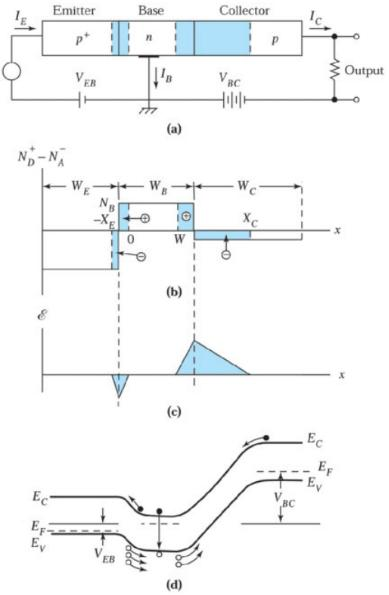
\includegraphics[width=8cm]{figures/ch01/bjt3.jpg}
\caption{pnp transistor in active mode} 
\label{fig:bjt3}
\end{figure}

\subsection{Courants en mode actif}
Pour chaque terminal, nous pouvons identifier les flux de porteurs qui contribuent aux courants $I_E$, $I_C$ et $I_B$.
\begin{enumerate}
	\item À l'émetteur :
	\begin{itemize}
		\item un courant de trous de l'émetteur vers la base $I_{Ep}$
		\item un flux d'électrons de la base vers l'émetteur $I_{En}$
	\end{itemize}
	Ainsi, $I_E = I_{Ep} + I_{En}$
	\item À la base :
	\begin{itemize}
		\item un courant $I_{BB}$ dû à la recombinaison de trous injectés avec des électrons (qui doivent être réapprovisionnés par la batterie). Ce courant équivaut à la différence entre $I_{Ep}$ et $I_{Cp}$ : $I_{BB} = I_{Ep} - I_{Cp}$
		\item un flux d'électrons de la base vers l'émetteur $I_{En}$
		\item un flux d'électrons du collecteur vers la base : $I_{Cn}$ (c'est-à-dire le courant de fuite de la jonction B-C polarisée en inverse)
	\end{itemize}
	Ainsi, $I_B = I_{En} + (I_{Ep} - I_{Cp}) - I_{Cn}$
	\item Au collecteur :
	\begin{itemize}
		\item un courant $I_{Cp}$ qui est ce qui reste de $I_{Ep}$ après le passage par la base.
		\item un flux d'électrons du collecteur vers la base par la jonction B-C polarisée en inverse : $I_{Cn}$
	\end{itemize}
	Ainsi, $I_C = I_{Cp} + I_{Cn}$
\end{enumerate}
Ces courants sont représentés sur la figure \ref{fig:bjt4}. Comme le suggère la figure, $I_{Ep}$ est le courant principal dans le dispositif.

\begin{figure}[h!]
\centering
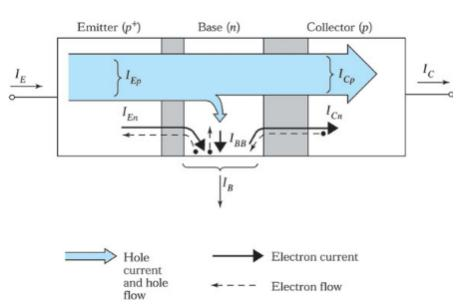
\includegraphics[width=11cm]{figures/ch01/bjt4.jpg}
\caption{Currents in active mode} 
\label{fig:bjt4}
\end{figure}

Nous caractérisons le transistor par le \emph{gain de courant en mode commun} $\alpha_0$, qui est le rapport entre $I_{Cp}$ et le courant d'émetteur :
$$
\alpha_0 \equiv \frac{I_{CP}}{I_E}
$$
Nous pouvons réécrire ceci comme :
$$
\alpha_0 = \frac{I_{Cp}}{I_{En} + I_{Ep}} = \Big(\frac{I_{Ep}}{I_{En} + I_{Ep}}\Big)  \Big(\frac{I_{Cp}}{I_{Ep}}\Big) = \alpha_T \; \gamma
$$
avec $\alpha_T$ le \emph{facteur de transfert de base} et $\gamma$ l'\emph{efficacité d'émetteur}. Pour un fonctionnement correct, nous exigeons que $I_{Ep} \gg I_{En}$, donc $\alpha_T \approx 1$. Cela peut être accompli en exigeant que le niveau de dopage de l'émetteur soit beaucoup plus élevé que celui de la base. Le facteur $\gamma$ peut être augmenté en diminuant la longueur de la base.\
Nous pouvons réécrire le courant de collecteur $I_C$ comme :
\begin{equation}
	\begin{split}
		I_C &= I_{Cp} + I_{Cn} = \alpha_T I_{Ep} = \alpha_0 I_E + I_{Cn} \\
		&= \alpha_0 I_E + I_{CB0}
	\end{split}
	\label{eq:bjt1}
\end{equation}
où $I_{CB0}$ est le courant de fuite entre le collecteur et la base avec la jonction émetteur-base ouverte. Cela exprime que le courant de collecteur est une fraction ($0 < \alpha_0 < 1$) du courant d'émetteur, plus un courant de fuite.

\subsection{Distribution de porteurs en mode actif}
Afin de calculer les différents courants, nous devons d'abord déterminer la distribution de porteurs dans chaque région. Nous supposerons ce qui suit :
\begin{enumerate}
	\item Dopage uniforme dans chaque région
	\item Pas de courant de dérive de trous dans la base
	\item Le courant de saturation du collecteur est négligeable
	\item Seulement une injection de faible niveau
	\item Pas de génération-recombinaison dans la zone de déplétion
	\item Pas de résistance série dans le dispositif
\end{enumerate}

Nous supposerons que $x=0$ correspond à la fin de la zone de déplétion émetteur-base, et $x=W$ au début de la zone de déplétion base-collecteur. À partir de l'équation de continuité pour les porteurs minoritaires dans la région de base:
$$
\frac{dp_n}{dt} = - \frac{(p_n-p_{n0})}{t_p} - \frac{1}{q} \frac{d J_p}{dx} + g \text{ avec }  J_p = q \mu_p p E + q D_p \frac{dp_n}{dx}
$$
Si nous supposons un état stationnaire, sans champ électrique et sans autres mécanismes de génération, l'équation se réduit à:
$$
D_p \frac{d^2 p_n}{dx^2} = \frac{(p_n-p_{n0})}{t_p}
$$
Cette équation a comme solution générale
$$
p_n(x) = p_{n0} + C_1  \; e^{x/L_p} + C_2 \;  e^{-x/L_p}
$$
avec $L_p = \sqrt{D_p t_p}$ la soi-disant \emph{longueur de diffusion} des trous dans le semi-conducteur de type n. Les constantes $C_1$ et $C_2$ peuvent être déterminées par les conditions aux limites:
\begin{itemize}
	\item $p_n(0) = p_{n0} ; e^{qV_{EB}/kT}$ car c'est la concentration standard à la limite de la région de déplétion, comme dans l'équation \ref{eq:density_junction} du chapitre \ref{ch:pnjunction},
	\item $p_n(W) = 0$ car tous les trous à $x=W$ seront balayés à travers la région de charge d'espace base-collecteur par le champ électrique induit.
\end{itemize}
La résolution pour $C_1$ et $C_2$ conduit à une distribution assez complexe. Cependant, si $W/L_p \ll 1$, nous pouvons simplifier et obtenir:
$$
p_n(x) = p_{n0}\; e^{qV_{EB}/kT} \; \Big(1 - \frac{x}{W} \Big)
$$
La concentration de porteurs minoritaires diminue donc linéairement dans la base. De manière similaire, nous pouvons trouver une expression pour les porteurs minoritaires (électrons) dans l'émetteur et le collecteur. Les résultats sont:
\begin{equation}
    \begin{split}
        n_E(x) &= n_{E0} + n_{E0} (e^{qV_{EB}/kT} - 1) e^{(x+x_E)/L_E}\\
        n_C(x) &= n_{C0} - n_{C0} e^{(x-x_C)/L_C}
    \end{split}
\end{equation}
Ces distributions sont également représentées dans la figure \ref{fig:bjt5}. Une fois que les concentrations de porteurs sont connues, les courants sont facilement calculés car ils sont proportionnels au gradient de concentration :
\begin{itemize}
    \item $I_{Ep} = A \Big(-q D_p \frac{dp_n}{dx}|_{x=0}\Big) = \frac{qAD_p \; p_{n0}}{W} e^{qV_{EB}/kT}$
    \item $I_{En} = A \Big(-q D_E \frac{dn_E}{dx}|_{x=-x_E}\Big) = \frac{qAD_E \; n_{E0}}{L_E} (e^{qV_{EB}/kT}-1)$
    \item \ldots
\end{itemize}
En combinant ces résultats, on obtient les expressions pour les trois courants terminaux :
\begin{itemize}
	\item $I_E = a_{11} (e^{qV_{EB}/kT} - 1) + a_{12}$
	\item $I_C = a_{12} (e^{qV_{EB}/kT} - 1) + a_{22}$
	\item $I_B = I_E - I_C$
\end{itemize}
où tous les $a_{ij}$ dépendent des caractéristiques du transistor comme les concentrations de dopage et les dimensions. 
\begin{figure}[h!]
\centering
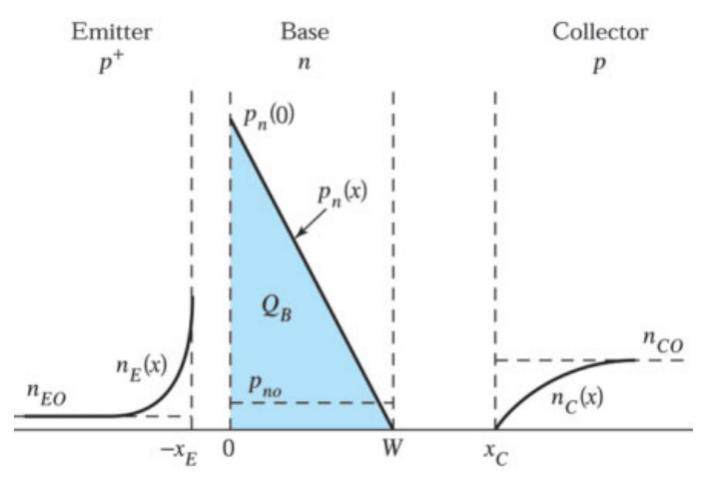
\includegraphics[width=10cm]{figures/ch01/bjt5.jpg}
\caption{Distribution de porteurs minoritaires en mode actif.} 
\label{fig:bjt5}
\end{figure}

\subsection{Modes de fonctionnement et équations d'Ebers-Moll}
\label{sec:modes_de_fonctionnement}
En fonction des signes de $V_{EB}$ et $V_{CB}$, nous pouvons distinguer $4$ modes de fonctionnement différents. Nous avons déjà étudié le cas où $V_{EB} > 0$ et $V_{CB} < 0$, à savoir le mode actif. Les autres modes sont représentés sur la figure \ref{fig:bjt_modes}, ainsi que la distribution des porteurs minoritaires dans l'émetteur, la base et le collecteur.
\begin{figure}[h!]
	\centering
	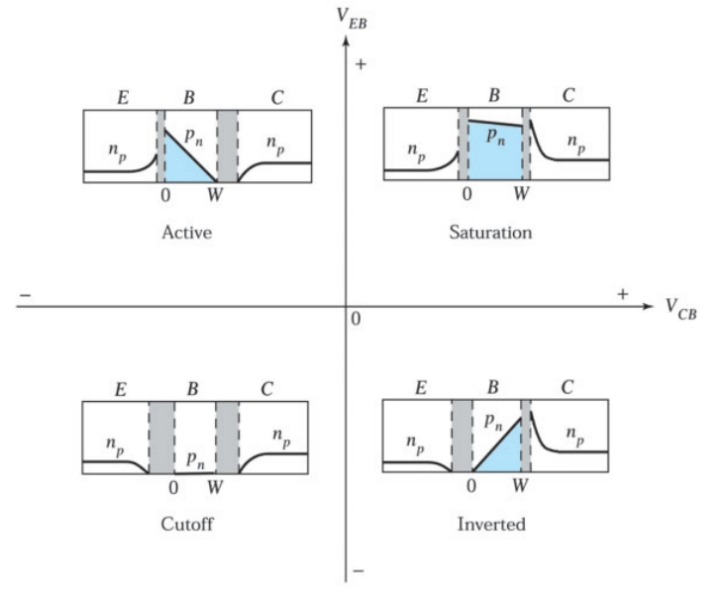
\includegraphics[width=12cm]{figures/ch01/bjt_modes.jpg}
	\caption{Modes de fonctionnement}
	\label{fig:bjt_modes}
\end{figure}
En mode saturation, les deux jonctions sont polarisées directement. La distribution de porteurs minoritaires à la limite de chaque région de déplétion n'est pas nulle, comme dans le mode actif. De faibles tensions de polarisation conduisent à un courant de sortie élevé. Le transistor agit comme un interrupteur fermé.\\
En mode coupure, les deux jonctions sont polarisées inversement. Seul un faible courant circulera. Le transistor est un interrupteur ouvert.\\
En mode inversé, l'émetteur et le collecteur sont inversés. Le comportement n'est cependant pas exactement comme dans le mode actif, car les niveaux de dopage dans l'émetteur et le collecteur sont différents.\\
Tous ces modes peuvent être analysés de manière similaire à ce que nous avons fait pour le mode actif. Cette analyse conduit aux \emph{équations d'Ebers-Moll} qui sont utilisées pour modéliser le BJT dans des simulateurs comme SPICE.\\
\textbf{TODO : Ajouter les équations d'Ebers-Moll et les circuits équivalents.}

\subsection{Configuration Émetteur Commun}
Jusqu'à présent, nous avons maintenu la base à une tension fixe. Cependant, l'utilisation la plus courante du transistor bipolaire est avec l'émetteur à une tension fixe comme dans la figure \ref{fig:bjt6}(a). Cette configuration a $V_{EB}$ et $I_B$ en entrée, et $I_C$ et $V_{EC}$ en sortie.\
Nous pouvons exprimer $I_C$ en fonction de $I_B$ en substituant $I_E = I_B + I_C$ dans l'équation \ref{eq:bjt1}:
$$
I_C = \alpha_0 (I_B + I_C) + I_{CBO}
$$
La résolution de l'équation \ref{eq:bjt1} pour $I_C$ donne:
\begin{equation}
    \begin{split}
        I_C &= \frac{\alpha_0}{1-\alpha_0} I_B + \frac{I_{CB0}}{1 - \alpha_0}\\
            &= \beta_0 I_B + I_{CE0}
        \label{eq:bjt2}
    \end{split}
\end{equation}
où $\beta_0 = \frac{\alpha_0}{1-\alpha_0}$ est le \emph{gain de courant commun-émetteur} et $I_{CE0} = \frac{I_{CB0}}{1-\alpha_0}$ est le courant de fuite collecteur-émetteur. Ce courant est toujours présent, même si $I_B = 0$, et rend le transistor bipolaire très mauvais comme interrupteur car il fuira du courant quand il est fermé.\\
Dans la configuration précédente, base commune, et avec $\alpha_0 \approx 1$, un changement du courant d'émetteur $I_E$ produit un changement d'environ la même quantité dans le courant de collecteur $I_C$ et un changement beaucoup plus petit dans le courant de base (facteur de $1-\alpha_0$). Pour obtenir une amplification de courant, le changement est initié dans le courant de base plutôt que dans le courant d'émetteur. Cela fait changer le courant de collecteur par un facteur de $\frac{\alpha_0}{1 - \alpha_0} = \beta_0$.\\
Lorsque $\alpha_0$ est proche de un, $\beta_0$ devient très grand. C'est une bonne chose car cela nous permet d'amplifier le courant de base $I_B$. Cependant, $\beta_0$ peut beaucoup varier d'un transistor à l'autre. C'est pourquoi nous explorerons des techniques de polarisation qui atténuent la variabilité de $\beta_0$.


\begin{figure}[h!]
\centering
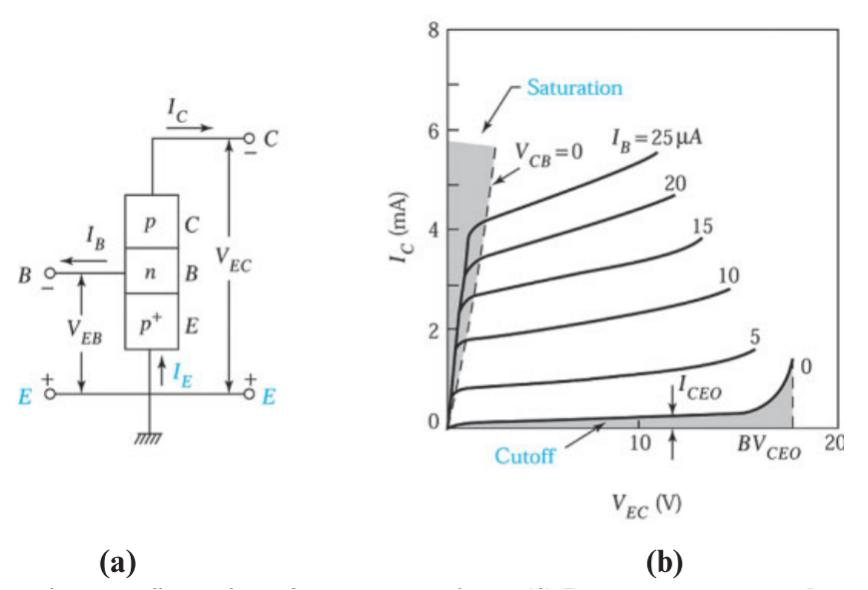
\includegraphics[width=10cm]{figures/ch01/bjt6.jpg}
\caption{BJT in common-emitter configuration (a) and I-V characteristic (b)} 
\label{fig:bjt6}
\end{figure}

La caractéristique I-V définissant une configuration émetteur commun est montrée dans la figure \ref{fig:bjt6}(b). Si $V_{EC}$ est trop faible, $V_{CB}$ est positif et la jonction base-collecteur n'est pas polarisée en inverse. Le transistor est en mode saturation. Ainsi, $V_{EC}$ doit être supérieur à un certain seuil pour mettre le transistor en mode actif. Cette valeur est appelée $V_{EC, Sat}$ et est d'environ $0,2$ V.\
Lorsque $V_{EC} > V_{EC, Sat}$, nous pouvons dire, sur la base de l'équation \ref{eq:bjt2}, que $I_C \approx \beta_0 I_B$ et donc indépendant de $V_{EC}$. C'est un comportement idéal, car nous contrôlons maintenant le courant de sortie $I_C$ avec le courant d'entrée $I_B$ et non avec la tension de sortie $V_{EB}$. Cependant, comme on peut le voir sur la figure, les caractéristiques I-V ne sont pas entièrement plates et dépendent donc encore de $V_{EB}$. Cela est dû à l'effet Early et sera abordé dans la prochaine section.\
Si $V_{EB}$ est inférieur à $0,6$ V, la jonction émetteur-base n'est pas polarisée en direct et $I_B$ est très faible. On dit que le transistor est en coupure. Le seul courant qui continue de circuler de l'émetteur vers le collecteur est le courant de fuite $I_{CE0}$.

\subsection{Effet Early}
En principe, $I_C$ devrait être indépendant de la tension de la jonction base-collecteur $V_{BC}$. Cependant, lorsque $V_{BC}$ augmente, la largeur de la région de charge d'espace entre la base et le collecteur augmente, comme prédit par l'équation \ref{eq:SCR_width_bias} où $V_F = -V_{BC}$. Cela signifie que la longueur effective de la base diminue et cela a deux effets :
\begin{enumerate}
	\item Plus de trous provenant de l'émetteur atteindront le collecteur car il y a moins de place pour la recombinaison. Effectivement, le facteur de transfert de base $\alpha_T$ augmente.
	\item Le courant de trou est déterminé par la pente de la concentration de trous dans la base, comme vu précédemment. Lorsque $W$ diminue, tout en maintenant les conditions aux limites, le courant de diffusion de trou $I_{Ep}$ augmente. L'augmentation de la pente (en termes absolus) est montrée dans la figure \ref{fig:bjt7}(a).
\end{enumerate}

Les deux effets contribuent à une augmentation de $I_C$ lorsque $V_{CB}$ (ou $V_{EC}$ en configuration émetteur commun) augmente et que $I_B$ reste constant. Ce phénomène est appelé l'\emph{effet Early}. Nous pouvons montrer que toutes ces courbes de courant non plates dans la caractéristique I-V (voir figure \ref{fig:bjt7}(b)) passent par le même point sur l'axe V lorsqu'elles sont étendues. La tension correspondante est la tension Early $V_A$.

\begin{figure}[h!]
\centering
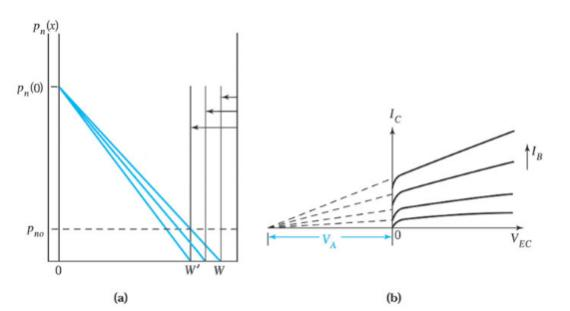
\includegraphics[width=10cm]{figures/ch01/bjt7.jpg}
\caption{Schematic diagram of (a) the Early effect and (b) Early voltage $V_A$} 
\label{fig:bjt7}
\end{figure}

%\section{Field-Effect Transistor}
%\newpage
%\section{JFET}
%PM

\newpage
\section{MOSFET}
\label{sec:mosfet}
Le transistor à effet de champ métal-oxyde-semi-conducteur, ou \emph{MOSFET}, est un transistor basé sur l'effet de champ. Il possède une grille isolée, constituée d'un conducteur tel que du métal ou du poly-silicium. Cette borne est isolée du reste du dispositif par une fine couche de $SiO_2$ qui sert de diélectrique. La tension appliquée à la grille détermine la conductivité du dispositif et peut donc contrôler le courant entre les deux autres bornes nommées source et drain. Cette capacité à modifier la conductivité en fonction de la tension appliquée peut être utilisée pour amplifier ou commuter des signaux électroniques. La Figure \ref{fig:mosfet1}(a) montre la structure d'un MOSFET, tandis que la Figure \ref{fig:mosfet1}(c) montre ses symboles ainsi que les trois bornes.
\subsection{Description et fonctionnement}
La Figure \ref{fig:mosfet1}(b) montre la section transversale d'un MOSFET à canal n. La source (S) et le drain (D) sont tous deux des contacts $n^+$ et sont isolés l'un de l'autre par le substrat de type p. Lorsque la tension sur la grille augmente, les trous dans le matériau de type p sont expulsés et la région sous la grille devient appauvrie en porteurs de charge. Si la tension de la grille augmente encore plus, les électrons présents dans le volume de type p en tant que porteurs minoritaires sont attirés vers la région sous la grille. Une couche étroite d'électrons entre la source et le drain est formée et la conduction d'électrons entre la source et le drain devient possible. Si la densité électronique sous la grille est égale à la concentration en trous dans le volume, une inversion s'est produite et nous disons qu'un canal s'est formé. La tension de la grille à laquelle cette inversion de type p à type n se produit est appelée tension seuil $V_T$.\
Pour qu'un courant s'écoule de la source au drain, nous avons besoin non seulement d'un canal, mais également d'une différence de tension positive entre le drain et la source. À mesure que nous augmentons la tension au niveau du drain, le courant augmente, mais en même temps, la profondeur du canal au niveau du drain diminue car $V_{GD} < V_{GS}$. À un certain moment, la différence de tension entre la grille et le drain n'est plus suffisante pour maintenir un canal de type n ($V_{GD} = V_T$). Nous appelons cela \emph{pinch-off} et disons que le transistor est saturé. Le courant entre le drain et la source n'augmente plus à mesure que la tension de drain augmente mais reste constant.

\begin{figure}[h!]
\centering
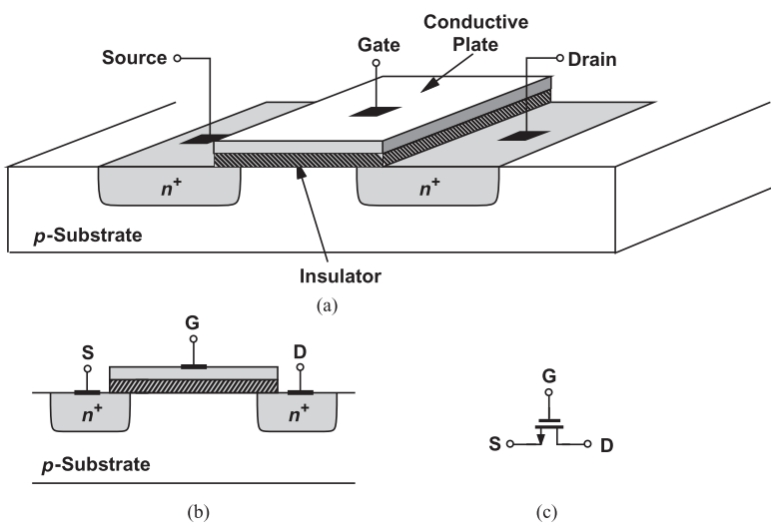
\includegraphics[width=10cm]{figures/ch01/mosfet1b.jpg}
\caption{Schematic diagram of a n-channel MOSFET: (a) structure, (b) side view, (c) symbol} 
\label{fig:mosfet1}
\end{figure}

Les dimensions d'un MOSFET peuvent devenir très petites ; l'épaisseur typique de l'oxyde de grille $t_{ox}$ est d'environ $15 \AA$ et diminue avec chaque nouvelle génération. La longueur du canal $L$ est généralement de plusieurs dizaines de nanomètres.

\subsection{Condensateur MOS}
La région sous la grille est appelée un condensateur MOS. Dans les circuits intégrés, il peut stocker des charges et constitue la base de construction pour les dispositifs à transfert de charges (CCD). Un MOSFET peut donc être considéré comme un condensateur MOS et deux jonctions pn placées immédiatement adjacentes. Nous verrons brièvement comment la charge s'accumule dans le semi-conducteur lorsqu'une tension est appliquée à la grille métallique.\
La figure \ref{fig:moscap} représente un condensateur MOS avec la grille à gauche et le semi-conducteur de type p à droite de l'oxyde. Si une tension négative $V < 0$ est appliquée à la plaque métallique de la grille, comme dans \ref{fig:moscap}(a), les porteurs positifs sont attirés vers l'interface $SiO_2 - Si$. Aucun courant ne circule dans le dispositif, donc le niveau de Fermi reste constant. La distribution des porteurs dépend de la différence $E_i - E_F$: $p_p = n_i e^{(E_i - E_F)/kT}$, donc les bandes de conduction et de valence à l'interface doivent se courber vers le haut pour augmenter $E_i - E_F$ car $E_F$ est constant. Les trous "flottent" vers le maximum dans la bande de valence et s'accumulent à l'interface.\
Si $V > 0$, comme dans \ref{fig:moscap}(b), les trous sont repoussés de l'interface et les bandes se courbent vers le haut. Au départ, tous les donneurs accepteurs sont exposés et une couche de charge de profondeur $W$ est créée à l'intérieur du semi-conducteur. La densité de charge induite par unité de surface est $Q_d = q N_A W$. Nous appelons ce processus \emph{déplétion}. Si $V$ augmente encore et que les bandes se courbent encore plus, le niveau de Fermi intrinsèque tombera en dessous du niveau de Fermi réel comme dans \ref{fig:moscap}(c) et les électrons afflueront vers l'interface car l'exposant dans l'expression $n_p = n_i e^{(E_F - E_i)/kT}$ devient positif. Ce processus est appelé \emph{inversion} et est la condition nécessaire pour former un canal dans un MOSFET. Le canal est une région très chargée juste à droite de l'interface (voir la distribution de charge), séparée du semi-conducteur de type p par une région de déplétion relativement large. La tension où les niveaux de Fermi se croisent est la tension de seuil $V_T$ et nous désignons la charge associée $Q_n$.

\begin{figure}[h!]
\centering
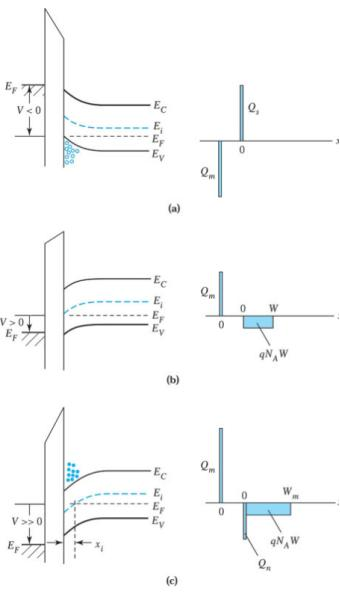
\includegraphics[width=7cm]{figures/ch01/moscap.jpg}
\caption{Band diagrams and charge distribution of a MOS capacitor in (a) accumulation, (b) depletion, and (c) inversion} 
\label{fig:moscap}
\end{figure}

\subsection{Caractéristique I-V}
\label{sec:MOS_IV}
Si $V$ est la différence de tension appliquée aux plaques d'un condensateur et $C$ la capacitance, alors la charge induite est $Q = CV$. Dans le cas du MOSFET de la figure \ref{fig:mosfet1}(b), nous ne nous intéressons qu'aux charges mobiles sous la grille, c'est-à-dire les électrons $Q_n$ attirés vers l'interface de la figure \ref{fig:moscap}(c), et non à la charge de déplétion $Q_d=qN_AW$. Cela signifie que $V=V_{GS}-V_T$ car aucune charge mobile n'existe pour $V_{GS}<V_T$ \footnote{Cette hypothèse sera révisée dans la section \ref{sec:subthreshold_conduction}}. Si nous supposons que le condensateur MOS a une capacité de grille $C_{ox}$ par unité de surface, cette relation devient
$$Q_n = W C_{ox} (V_{GS} - V_T)$$
avec $W$ la largeur du transistor. Notez que $Q_n$ est une densité de charge par unité de longueur. Comme la tension de drain et de source n'est pas la même, la tension de canal varie le long de la longueur du canal. Si nous désignons le potentiel de canal par $V(x)$, nous pouvons réécrire l'équation ci-dessus comme suit:
$$Q_n(x) = W C_{ox} (V_{GS} - V(x) - V_T)$$
où $V(x)$ va de zéro à $V_D$ si le canal n'est pas étranglé (figure \ref{fig:mosfet2}(a)).\\
Nous savons que le courant est la densité de charge multipliée par la vitesse des charges: $I_D=Q_n(x)\cdot v$. Le courant est un courant de dérive car nous appliquons un champ électrique $\mathcal{E}$ à travers le canal. Ainsi :
$$v = -\mu_n \mathcal{E} = \mu_n \frac{dV}{dx}$$
avec $\mu_n$ la mobilité des électrons. En substituant cela dans l'expression de $I_D$, nous trouvons :
$$I_D = W C_{ox} (V_{GS} - V(x) - V_T) \mu_n \frac{dV(x)}{dx}$$
En multipliant les deux côtés par $dx$ et en intégrant de $x = 0$ à la longueur de canal $L$ :
$$
 \int_{x=0}^{x=L} I_D dx = \int_{V(x)=0}^{V(x)=V_{DS}} \mu_n C_{ox} W (V_{GS}-V(x)-V_T)dV 
$$
Parce que $I_D$ est constant le long du canal, nous pouvons résoudre les deux intégrales et exprimer $I_D$ comme
\begin{equation}
\begin{split}
    I_D = \frac{1}{2} \mu_n C_{ox} \frac{W}{L} [ 2(V_{GS} - V_T) V_{DS} - V_{DS}^2 ]
\end{split}
\end{equation}
Ceci est une fonction parabolique qui atteint un maximum pour $V_{DS} = V_{GS} - V_T$ :
$$I_{D, max} = \frac{1}{2} \mu_n C_{ox} \frac{W}{L} (V_{GS} - V_T)^2$$
Nous avons déjà établi que la condition de saturation est $V_{GD} = V_T$ : à partir de ce point, le courant ne va plus augmenter lorsque $V_{DS}$ augmente car un effet de pincement s'est produit au drain. Étant donné que $V_{DG} = V_{DS} - V_{GS}$ et que lorsqu'un effet de pincement se produit $V_{DG} = -V_T$, nous pouvons réécrire cette condition sous la forme $V_{DS} = V_{GS} - V_T$, c'est-à-dire que le transistor est en saturation au maximum de la courbe. C'est la situation représentée dans la figure \ref{fig:mosfet2}(b) et (c). Lorsque $V_{DS}$ augmente, le point de pincement $P$ se rapproche de la source. La différence de potentiel dans le canal rétrécissant en $P$ reste à $V_{GS} - V_T$. Le transistor est en saturation\footnote{Notez que la saturation pour un MOSFET n'est pas le même concept que la saturation pour un BJT} et le courant de drain est - dans une première approximation - égal à :
\begin{equation}
    I_{D} = \frac{1}{2} \mu_n C_{ox} \frac{W}{L} (V_{GS} - V_T)^2
    \label{eq:sat_current}
\end{equation}
Notez que contrairement au BJT, il n'y a pas de courant continu à travers la grille.\footnote{Note sur la notation : nous utiliserons souvent $K$ pour le produit $\mu_n C_{ox}$.}

\begin{figure}[h!]
\centering
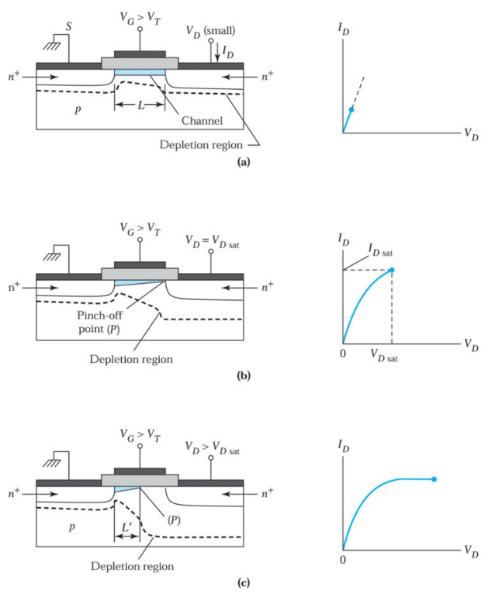
\includegraphics[width=12cm]{figures/ch01/mosfet2.jpg}
\caption{Operations of the MOSFET and output I-V characteristics. (a) Low drain voltage. (b) Onset of saturation. (c) Beyond saturation.} 
\label{fig:mosfet2}
\end{figure}

Si $V_{DS}$ est relativement petit, nous pouvons approximer $I_D$ comme suit :
$$I_D \approx  \mu_n C_{ox} \frac{W}{L} (V_{GS} - V_T) V_{DS}$$
Ceci est l'expression d'une résistance avec une valeur:
$$R_{on} = \frac{1}{\mu_n C_{ox} \frac{W}{L} (V_{GS} - V_T)}$$
Nous disons que le transistor est dans la région \emph{linéaire} ou \emph{triode}. Comme la résistance est une fonction de $V_{GS}$, le MOSFET dans cette région peut être considéré comme une résistance programmable.
%$$I_{D} = \frac{1}{2} \mu_n C_{ox} \frac{W}{L} (V_{GS} - V_T)^2$$

La figure \ref{fig:mosfet3} donne la caractéristique de sortie globale d'un MOSFET à canal N. Remarquez comment le point de transition de linéaire à saturation dépend de $V_{GS}$ : pour que le transistor soit en saturation, $V_{DS}$ doit être plus grand que la \emph{tension de suralimentation} $V_{ov} = V_{GS} - V_T$, également appelée tension de saturation $V_{DS, Sat}$. Ce n'est pas le cas pour le BJT, où nous avons utilisé une coupure fixe $V_{CE,sat}$ avec une valeur de $0,2$ V.

\begin{figure}[h!]
\centering
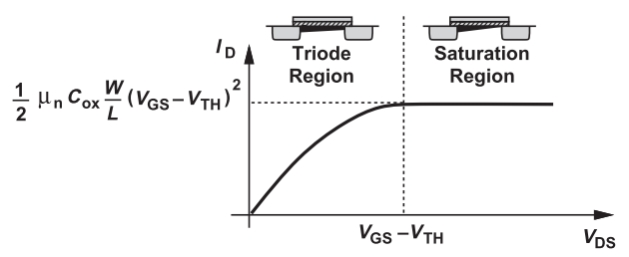
\includegraphics[width=10cm]{figures/ch01/mosfet3.jpg}
\caption{Overall MOSFET $I_D - V_{DS}$ characteristic} 
\label{fig:mosfet3}
\end{figure}
Nous avons étudié le MOSFET à canal N ou \emph{NMOS}. L'étude du MOSFET à canal P ou \emph{PMOS} est laissée en exercice pour le lecteur.

\subsection{Effets de Second Ordre}
Nous discuterons de plusieurs effets de second ordre qui feront que le MOSFET se comportera différemment du comportement idéal de la figure \ref{fig:mosfet3}.
\subsubsection{Modulation de la longueur du canal}
Remarquez que dans la figure \ref{fig:mosfet3}(c), la longueur effective du canal diminue à mesure que la tension de drain augmente (le point d'étranglement se déplace vers la gauche). Nous avons établi l'équation \ref{eq:sat_current} avec l'hypothèse implicite que $L$ est constant. Cependant, si la longueur effective du canal diminue, le courant $I_D$ augmentera avec l'augmentation de $V_{DS}$ et la caractéristique I-V de la figure \ref{fig:mosfet3} ne sera pas plate. Ceci est similaire à l'effet Early dans le BJT.\
Pour modéliser cela, nous supposons que $L$ ne change pas, mais incluons une dépendance explicite de $V_{DS}$ dans l'équation \ref{eq:sat_current} :
\begin{equation}
    I_{D} = \frac{1}{2} \mu_n C_{ox} \frac{W}{L} (V_{GS} - V_T)^2 \; (1 + \lambda V_{DS})
    \label{eq:sat_current2}
\end{equation}
Le facteur $\lambda$ est le \emph{coefficient de modulation de longueur de canal}. Pour diminuer $\lambda$, le concepteur peut augmenter la longueur du transistor, car cela rend l'impact relatif d'un changement de $L$ plus petit.
\subsubsection{Effet de corps}
Jusqu'à présent, nous avons supposé que le substrat de type p et la source de type n étaient connectés à une masse commune. Ce n'est cependant pas toujours le cas dans les circuits réels, où la source peut être connectée à des tensions supérieures à celles du substrat. Même dans ce cas, la jonction pn entre la source et le substrat est toujours polarisée en inverse et le dispositif fonctionne correctement.\\
Cependant, quelque chose change lorsque la tension de la source augmente par rapport au substrat: lorsque la source devient plus positive par rapport au substrat, la tension de seuil $V_T$ augmente. Appelé "effet de corps", ce phénomène est formulé comme
$$V_T = V_{T0} + \gamma (|2\phi_F + V_{SB} - |2\phi_F|)$$
où $V_{SB}$ est la différence de tension entre la source et le substrat (bulk), $V_{T0}$ est la tension de seuil lorsque $V_{SB} = 0$ et $\gamma$ et $\phi_F$ sont des paramètres dépendants de la technologie.
\subsubsection{Conduction sub seuil}
\label{sec:subthreshold_conduction}
Nous avons supposé que le MOSFET s'allume brusquement lorsque la tension de la grille dépasse la tension de seuil. En pratique cependant, le dispositif s'allume progressivement et il y a déjà un courant source-drain avant que $V_T$ soit atteint. Ce courant dépend exponentiellement de $V_{GS}$, de manière similaire à un BJT. Appelé la \emph{conduction sub seuil}, cet effet est devenu un problème critique dans les dispositifs MOS modernes.
\part{Électronique analogique}
\chapter{Circuits Analogiques de Base}
Dans ce chapitre, nous verrons comment les éléments non linéaires sont utilisés dans les circuits électriques. Nous discuterons du concept d'une droite de charge, à la fois statique et dynamique, et étudierons la réponse en petit signal d'un élément non linéaire, ce qui nécessite essentiellement une linéarisation autour d'un point de fonctionnement. Enfin, nous fournirons des modèles en petit signal pour les diodes et les transistors à hautes et basses fréquences.

\section{Éléments non linéaires dans les circuits}
\label{sec:nonlin_circuits}
Dans cette section, nous verrons comment les éléments non linéaires tels que les diodes et les transistors sont utilisés dans les circuits électriques. En principe, l'ajout d'un élément non linéaire rend l'analyse du circuit beaucoup plus difficile que les circuits avec seulement des éléments linéaires (résistances, condensateurs, inductances, \ldots). En pratique cependant, nous nous appuierons sur une méthode de résolution graphique, qui simplifie l'analyse tout en restant rigoureuse.
\subsection{La Diode comme Élément de Circuit}
Utilisons une diode comme élément discret dans un circuit électronique, comme dans la figure ci-dessous.

\begin{wrapfigure}{r}{3.5cm}
	\centering
	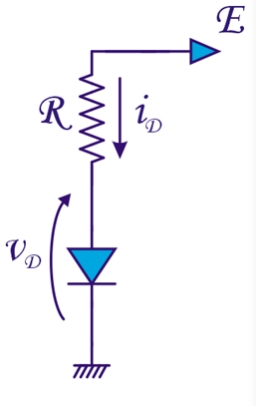
\includegraphics[width=3cm]{figures/ch02/diode1.jpg}
	\caption{}
	\label{fig:diode1}
\end{wrapfigure}
En appliquant la LKV, nous obtenons l'équation de la \textbf{droite de charge}:
$$
E - v_D = R \; i_D
$$
Cette équation doit être combinée avec la caractéristique I-V de la diode:
$$
i_D = \phi(v_D) = I_S (e^{v_D/v_{th}} - 1)
$$
D'un point de vue formel, nous avons deux inconnues, $v_D$ et $i_D$, et deux équations, donc en principe, nous pouvons résoudre pour les deux inconnues. Cependant, il n'y a pas de solution analytique à notre problème, nous préférons donc une méthode graphique.\
Dans la figure \ref{fig:diode2}, nous combinons $i_D = \phi(v_D)$ (la courbe rouge) avec l'expression de la droite de charge (la ligne verte).

\begin{figure}[h!]
	\centering
	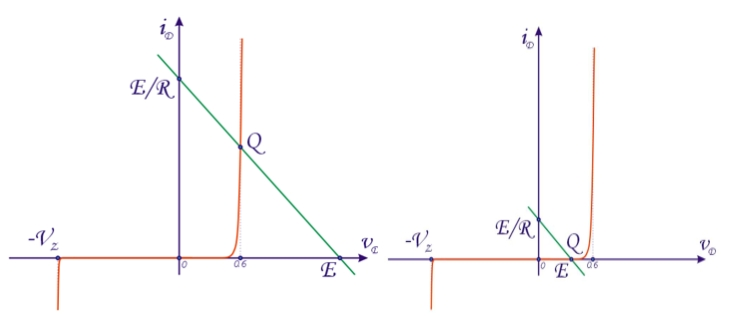
\includegraphics[width=12cm]{figures/ch02/diode2.jpg}
	\caption{I-V avec ligne de charge (a) avec $E > 0.6 V$ et (b) $E < 0.6$ V}
	\label{fig:diode2}
\end{figure}
Nous appliquons une simplification et supposons que $v_D = V_{DQ} \approx 0,6$ V. Le point de fonctionnement\footnote{La lettre $Q$ signifie \emph{quiescent}} $Q$ se situe à l'intersection des deux lignes. Pour que la diode conduise, nous pouvons immédiatement conclure, en comparant les deux figures, qu'il est nécessaire que $E > 0,6$ V $= V_{DQ}$. Le courant dans la diode est facilement calculé comme
$$
i_D \approx I_{DQ} = \frac{E - V_{DQ}}{R}
$$
Nous pouvons conclure que la diode conduira toujours tant que $E > 0,6$ V. Les variations de $E$ signifient seulement que la droite de charge se déplacera parallèlement. Le point de fonctionnement $(V_{DQ}, I_{DQ})$ ne peut se déplacer que verticalement en raison de la nature de $\phi(v_D)$ lorsque $v_D > 0,6$ V. Seulement lorsque $E$ devient inférieur à $0,6$ V la conduction s'arrête jusqu'à ce que nous atteignions la région Zener. Rappelons que le $0,6$ V est spécifique pour le silicium.\\

\begin{minipage}{.6\textwidth}
	Considérons par exemple le circuit de la figure \ref{fig:diode3}. Il n'est pas évident de savoir quand la diode va conduire, donc remplaçons la source de courant et la résistance par l'équivalent de Thévenin, à savoir une résistance $R_{th} = R$ et une source de tension $V_{th} = R I_0$ en \textbf{série} avec cette résistance. Ce circuit est identique à celui de la figure \ref{fig:diode1} avec une droite de charge passant par les points $(R;I_0, 0)$ et $(0, I_0)$. On peut conclure que la diode va conduire lorsque $V_{th} = R;I_0 > 0,6$ V. De plus, lorsque $R\rightarrow \infty$ et que la résistance devient un circuit ouvert, la droite de charge deviendra une ligne horizontale passant par $I_0$.
\end{minipage}
\begin{minipage}{.5\textwidth}
	\centering
	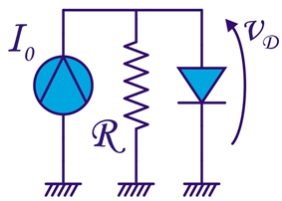
\includegraphics[width=5cm]{figures/ch02/diode3.jpg}
	\captionof{figure}{Avec source de courant}
	\label{fig:diode3}
\end{minipage}%

\subsection{Le BJT en tant qu'élément de circuit}
Un circuit typique à transistor bipolaire est représenté sur la figure \ref{fig:bjt_load1}(b). Pour analyser ce circuit, nous effectuons une coupure à l'entrée de la base et remplaçons la boucle de résistances $R_1$ et $R_2$ ainsi que la tension d'alimentation $E$ par le circuit équivalent de Thévenin, représenté sur la figure \ref{fig:bjt_load1}(a).

\begin{figure}[h!]
	\centering
	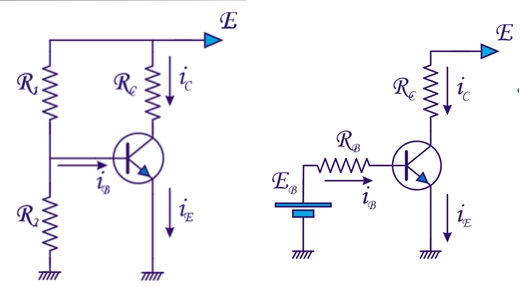
\includegraphics[width=12cm]{figures/ch02/bjt_load1.jpg}
	\caption{(a) Circuit à transistor et (b) simplifié avec Thévenin}
	\label{fig:bjt_load1}
\end{figure}

La tension de Thévenin $E_B$ et l'impédance $R_B$ peuvent être facilement calculées en observant que (a) la tension à la base est le résultat de l'application d'un diviseur de tension à la tension d'alimentation $E$, et (b) que lorsque nous mettons à la masse la tension $E$ (comme requis par les règles de Thévenin), $R_1$ et $R_2$ sont en parallèle :
\begin{equation}
	\begin{split}
		E_B &= \frac{R_2}{R_1 + R_2} E \\
		R_B &= R_1 || R_2 = \frac{R_1 R_2}{R_1 + R_2}
	\end{split}
\end{equation}
Dans cette boucle de gauche, nous pouvons écrire :
\begin{equation}
	\begin{split}
		E_B - v_{BE} &= R_B \; i_B \\
		%E - v_{CE} &= R_C \; i_C
	\end{split}
\end{equation}
Considérons la boucle de droite, qui est composée de la résistance $R_C$ et de la tension $v_{CE}$. Dans cette boucle, nous pouvons écrire :
\begin{equation}
	\begin{split}
		%E_B - v_{BE} &= R_B \; i_B \\
		E - v_{CE} &= R_C \; i_C
	\end{split}
\end{equation}
Supposons que tous les courants sont constants et que le transistor est polarisé dans son point de fonctionnement. Nous indiquons cela en ajoutant un $Q$ aux courants et tensions, tout comme pour la diode. Avec cette convention, nous pouvons réécrire ces équations pour obtenir :
\begin{equation}
	\begin{split}
		I_{BQ} &= \frac{E_B - V_{BEQ}}{R_B}\\
		V_{CEQ} &= E - R_C ; I_{CQ}
	\end{split}
\end{equation}
avec $V_{BEQ} \approx 0.6$ V car nous voulons polariser la jonction base-émetteur dans la région avant (conductive). À partir de l'analyse de la diode, nous savons que ce sera le cas lorsque $E_B > 0.6$ V. Nous connaissons également la relation entre $I_{BQ}$ et $I_{CQ}$ (en négligeant tout courant de fuite) :
\begin{equation}
	\begin{split}
		I_{CQ} &= \beta \; I_{BQ}
	\end{split}
\end{equation}
où $\beta$ est donné par le fabricant et est généralement très élevé, mais peut varier beaucoup d'un transistor à l'autre. Avec cette équation, nous avons suffisamment d'informations pour calculer tous les courants et tensions :
\begin{enumerate}
	\item Nous connaissons $R_B$ et $E_B$, et nous supposons que $V_{BEQ} = 0.6$ V, donc nous pouvons calculer $I_{BQ}$.
	\item Nous connaissons $\beta$, donc nous pouvons calculer $I_{CQ}$.
	\item Nous pouvons maintenant calculer $V_{CE}$.
\end{enumerate}
Tous ces calculs peuvent être représentés graphiquement ; voir la caractéristique (idéalisée) du BJT dans la figure \ref{fig:bjt_load2}.
\begin{figure}[h!]
	\centering
	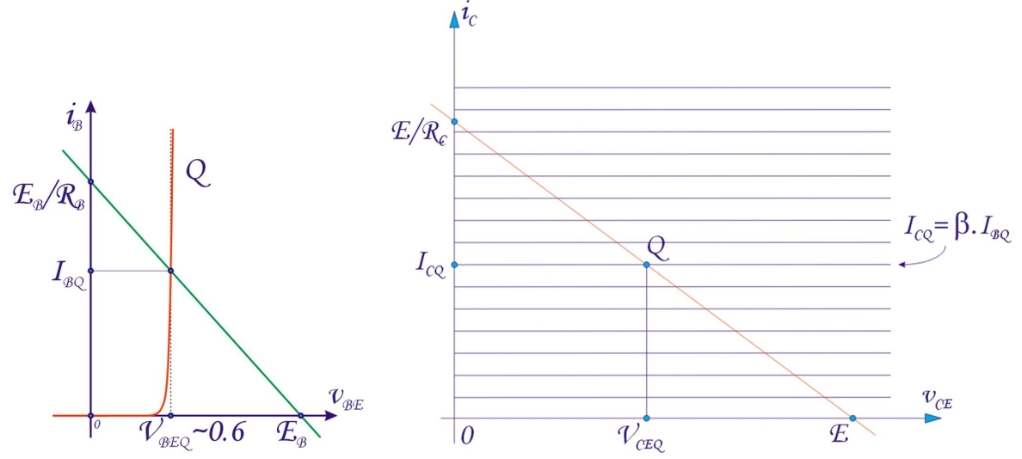
\includegraphics[width=12cm]{figures/ch02/bjt_load2.jpg}
	\caption{(a) Transistor circuit and (b) simplified with Thevenin} 
	\label{fig:bjt_load2}
\end{figure}
La figure de gauche représente la boucle de gauche, avec la droite de charge $E_B - v_{BE} = R_B ; i_B$ en vert et la caractéristique de la jonction $v_{BE}$ en rouge. L'intersection entre les deux fonctions est le point de fonctionnement $Q = (V_{BEQ}, I_{BQ})$. \
La boucle de droite est montrée dans le graphique de droite ; la ligne horizontale sur laquelle le transistor fonctionne est donnée par $I_{C} = \beta ; I_{B}$ et la droite de charge est donnée par $V_{CE} = E - R_C ; I_{C}$. Encore une fois, le point de fonctionnement est là où les deux lignes se croisent. \
Nous pouvons raisonner sur le fonctionnement du circuit en réfléchissant à ces figures. Par exemple, si $R_B$ diminuait, la pente de la droite de charge $I_B - V_{BE}$ augmenterait, de sorte que le point de fonctionnement $Q$ se déplacerait vers le haut et $I_{BQ}$ augmenterait. Cette augmentation provoquera une augmentation de $I_{CQ}$ dans le graphique de droite, et le point de fonctionnement se déplacera le long de la droite de charge vers un $I_C$ plus élevé et un $V_{CE}$ plus bas. \
Nous pouvons en conclure que :
\begin{itemize}
	\item La boucle de gauche détermine $I_{BQ}$.
	\item Par hypothèse, nous sommes dans le domaine de fonctionnement normal et $I_{CQ} = \beta I_{BQ}$.
	\item La boucle de droite donne $V_{CEQ}$.
	\item Étant donné $Q = (V_{CEQ}, ; I_{CQ})$, nous vérifions que nous sommes dans le domaine de fonctionnement normal.
\end{itemize}
Discutons maintenant de quelques cas limites :
\begin{itemize}
	\item Si $E_B < 0,6$ V, alors $V_{BEQ} < 0,6$ V. Alors $I_{BQ} \approx 0$ et $I_{CQ} \approx 0$ (en négligeant le courant de fuite). Voir la figure \ref{fig:bjt_load3}(a). Dans ce cas, le point de fonctionnement est $Q = (V_{CEQ} = E, 0)$ et le transistor est bloqué (\emph{mode de coupure}).
	\begin{figure}[h!]
		\centering
		\includegraphics[width=14cm]{figures/ch02/bjt_load3.jpg}
		\caption{(a) $V_{BEQ} < 0.6$V et (b) $V_{CEQ} \approx V_{CE, Sat}$}
		\label{fig:bjt_load3}
	\end{figure}
	\item Au fur et à mesure que $V_{BEQ}$ et $I_{BQ}$ augmentent, $I_{CQ}$ deviendra plus grand et éventuellement $V_{CEQ}$ deviendra trop petit pour maintenir le transistor en mode actif. Ensuite, $I_{CQ} \ne \beta ;I_{BQ}$ et $V_{CEQ} \approx V_{CE, Sat}$. Dans ce cas, $I_{CQ} = \frac{E-V_{CE,Sat}}{R_C}$. Le transistor est \emph{saturé}.
\end{itemize}

\subsection{Le MOSFET en tant qu'élément de circuit}
Tout comme pour le BJT, nous considérons un circuit de polarisation pour le transistor MOSFET à canal n tel que présenté dans la figure \ref{fig:mos_load1}(a) et nous simplifions le circuit avec un circuit équivalent de Thévenin - comme nous l'avons fait auparavant - comme dans la figure \ref{fig:mos_load1}(b).
\begin{figure}[h!]
	\centering
	\includegraphics[width=10cm]{figures/ch02/mos_load1.jpg}
	\caption{(a) Circuit de transistor MOS et (b) simplifié avec Thévenin}
	\label{fig:mos_load1}
\end{figure}
avec
\begin{equation}
	\begin{split}
		E_B-G &= \frac{R_2}{R_1 + R_2} E \\
		R_G &= R_1 || R_2 = \frac{R_1 R_2}{R_1 + R_2}
	\end{split}
\end{equation}
Notez que le courant de la grille $I_G = 0$ car la grille est un condensateur où le courant continu est nul. Et tout comme pour le BJT, nous pouvons exprimer une équation pour la boucle gauche et droite :
\begin{equation}
	\begin{split}
		V_{GSQ} &= E_G \text{ car } I_{G} = 0\\
		I_{DSQ} &= \frac{\mu_n C_{ox}}{2} \frac{W}{L} (V_{GSQ} - V_T)^2 \text{ si } V_{GSQ} > V_T\\
		V_{DSQ} &= E - R_D ; I_{DSQ} \text{ si } V_{DSQ} > V_{GSQ} - V_T
	\end{split}
\end{equation}
La dernière condition est requise pour que le transistor soit saturé, ce qui est similaire au mode actif pour un BJT.\\
Nous pouvons également représenter ces équations graphiquement. La figure \ref{fig:mos_load2}(a) représente la relation quadratique entre $I_{DS}$ et $V_{GS}$ pour déterminer $V_{GSQ}$. Tant que $V_{DS} > V_{GSQ} - V_T$, la figure \ref{fig:mos_load2}(b) donne la valeur de $V_{DSQ}$.
\begin{figure}[h!]
	\centering
	\includegraphics[width=14cm]{figures/ch02/mos_load2.jpg}
	\caption{(a) $i_{DS} = f(v_{DS})$ et (b) $I_{DS} = f(V_{DS})$}
	\label{fig:mos_load2}
\end{figure}


\subsection{Remarques supplémentaires}
Pour les deux types de transistors, il y a trois domaines de fonctionnement, comme indiqué dans la figure \ref{fig:transistor_overview}:
\begin{itemize}
	\item MOSFET : bloqué, saturé, linéaire
	\item BJT : bloqué, normal (ou actif), saturé
\end{itemize}
\begin{figure}[h!]
	\centering
	\includegraphics[width=12cm]{figures/ch02/overview.jpg}
	\caption{(a) $i_{DS} = f(v_{DS})$ et (b) $I_{DS} = f(V_{DS})$}
	\label{fig:transistor_overview}
\end{figure}
\subsection{Un circuit plus général}
\label{sec:general_circuit}
Pour améliorer la linéarité (voir le chapitre sur la rétroaction) et le polarisation du circuit, une résistance d'émetteur $R_E$ est souvent ajoutée, comme indiqué dans la figure \ref{fig:general1a}. Tout comme précédemment, le côté gauche est simplifié avec l'équivalent de Thévenin (voir \ref{fig:general1b}).

\begin{figure}[h!]
	\centering
	\begin{minipage}{.5\textwidth}
		\centering
		\includegraphics[width=4cm]{figures/ch02/general1a.jpg}
		\captionof{figure}{Circuit général}
		\label{fig:general1a}
	\end{minipage}%
	\begin{minipage}{.5\textwidth}
		\centering
		\includegraphics[width=5cm]{figures/ch02/general1b.jpg}
		\captionof{figure}{Simplification de Thévenin}
		\label{fig:general1b}
	\end{minipage}
	% \label{fig:explore}
\end{figure}
Encore une fois, nous pouvons écrire la LKC dans la boucle gauche et droite :
\begin{equation}
	\begin{split}
		E_B - V_{BEQ} &= R_B I_{BQ} + R_E I_{EQ} = R_B I_{BQ} + R_E (\beta + 1) I_{BQ} \\
		E_B - V_{BEQ} &= R_B \frac{I_{CQ}}{\beta} + R_E (\beta + 1) \frac{I_{CQ}}{\beta} \approx \frac{R_B}{\beta} I_{CQ} + R_E I_{EQ}
	\end{split}
\end{equation}
où nous avons utilisé $I_{CQ} = \beta I_{BQ}$ car nous supposons que nous travaillons dans la région de fonctionnement normal. Ces équations conduisent à des expressions pour le courant $I_{CQ}$ et la tension $V_{CEQ}$ :
\begin{equation}
	\begin{split}
		I_{CQ} &= \frac{E_B - V_{BEQ}}{\frac{R_B}{\beta} + R_E}\\
		V_{CEQ} &= E - (R_C + R_E) I_{CQ}
	\end{split}
	\label{eq:four_resitors1}
\end{equation}
Ils peuvent être tracés sur les différentes caractéristiques I-V comme sur la figure \ref{fig:general2}. Remarquez que la figure de gauche donne $i_C$ en fonction de $v_{BE}$. Puisque la relation entre $i_B$ et $v_{BE}$ est la caractéristique exponentielle de la diode, il en va de même pour la relation entre $i_C = \beta i_B$ et $v_{BE}$.

\begin{figure}[h!]
	\centering
	\includegraphics[width=12cm]{figures/ch02/general2.jpg}
	\caption{(a) Droite de charge : $I_{CQ} = \frac{E_B - V_{BEQ}}{\frac{R_B}{\beta} + R_E}$ (b) $V_{CEQ} = E - (R_C + R_E) I_{CQ}$}
	\label{fig:general2}
\end{figure}

On peut appliquer le même raisonnement au circuit MOSFET à $4$ résistances de la figure \ref{fig:mos_load3}, pour lequel nous pouvons également simplifier la boucle de gauche avec l'équivalent de Thévenin de la figure \ref{fig:mos_load4}.
\begin{figure}[h!]
	\centering
	\begin{minipage}{.5\textwidth}
		\centering
		\includegraphics[width=5cm]{figures/ch02/mos_load3.jpg}
		\captionof{figure}{}
		\label{fig:mos_load3}
	\end{minipage}%
	\begin{minipage}{.5\textwidth}
		\centering
		\includegraphics[width=6cm]{figures/ch02/mos_load4.jpg}
		\captionof{figure}{}
		\label{fig:mos_load4}
	\end{minipage}
	%	\label{fig:explore}
\end{figure}
Le point de fonctionnement $Q$ est déterminé par:
\begin{align*}
	&\text{L'équation de la boucle de gauche: } E_G - V_{GSQ} = R_S I_{DSQ} \
	&\text{La caractéristique du transistor: } I_{DSQ} = \frac{K}{2}\frac{W}{L} (V_{GSQ} - V_T)^2 \
	&\text{L'équation de la boucle de droite: } V_{DSQ} = E - (R_D + R_S)I_{DSQ}
\end{align*}
Pour trouver $V_{GSQ}$ et $I_{DSQ}$, utilisez les deux premières équations ; seule une racine est valide pour $V_{GSQ}$. $V_{DSQ}$ découle immédiatement de la troisième équation.
\section{Réponse en petit signal}
\label{sec:small_signal_response}
Dans cette section, nous allons introduire le concept de réponse en petit signal, c'est-à-dire comment les tensions et les courants dans un circuit changent lorsque nous appliquons une petite variation aux valeurs d'entrée. L'idée générale est que nous concevons le circuit de sorte qu'il fonctionne à un point de fonctionnement $Q$, et nous linéarisons le circuit autour de ce point de fonctionnement pour n'étudier que de petites déviations. Nous utiliserons la diode comme exemple. Dans la section \ref{sec:small_signal_model}, nous appliquons le même raisonnement aux transistors.\
Tout d'abord, nous introduisons une notation pour distinguer les quantités de grand signal des quantités de petit signal.

\begin{figure}[h!]
	\centering
	\includegraphics[width=8cm]{figures/ch02/small_signal_resp1.jpg}
	\caption{Signal quantities}
	\label{fig:small_signal_resp1}
\end{figure}
\begin{itemize}
	\item $x_A$: mesure d'une variable spécifique,
	\item $X_A$: la valeur moyenne de cette variable spécifique,
	\item $x_a$: variation de la variable spécifique autour de la moyenne $X_A$.
\end{itemize}
Consultez la figure \ref{fig:small_signal_resp1} pour une représentation visuelle de ces variables. Notez que seuls $x_A$ et $x_a$ varient dans le temps et que la valeur moyenne de $x_a$ est nulle : $\mathds{E}[x_a] = 0$.

\begin{minipage}{.6\textwidth}
	Appliquons cela au circuit diode simple. Dans la figure \ref{fig:small_signal_resp2}, l'alimentation comporte deux composantes : une tension fixe $E$, et une tension variable $e$ avec une valeur moyenne $\mathds{E}[e(t)] = 0$. Les quantités que nous recherchons, $v_D$ et $i_D$, peuvent être divisées en deux composantes : une valeur moyenne et une variation autour de cette moyenne.
	\begin{equation}
		\begin{split}
			v_D &= V_D + v_d\\
			i_D &= I_D + i_d
		\end{split}
	\end{equation}
\end{minipage}
\begin{minipage}{.4\textwidth}
	\centering
	\includegraphics[width=5cm]{figures/ch02/small_signal_resp2.jpg}
	\captionof{figure}{}
	\label{fig:small_signal_resp2}
\end{minipage}

Supposons que $e=0$, c'est-à-dire que nous étudions le système sans variations. Si $E>0.6V$, nous pouvons écrire - comme nous l'avons fait précédemment - que :
\begin{equation}
	\begin{split}
		V_{DQ} &= 0.6V\\
		I_{DQ} &= \frac{E-V_{DQ}}{R}
	\end{split}
\end{equation}
Ainsi, nous déterminons le point de fonctionnement comme l'intersection entre la droite de charge et la caractéristique de la diode, comme dans la figure \ref{fig:small_signal_resp4}..

\begin{figure}[h!]
	\centering
	\begin{minipage}{.5\textwidth}
		\centering
		\includegraphics[width=6cm]{figures/ch02/small_signal_resp4.jpg}
		\captionof{figure}{Diode equation and load line}
		\label{fig:small_signal_resp4}
	\end{minipage}%
	\begin{minipage}{.5\textwidth}
		\centering
		\includegraphics[width=6cm]{figures/ch02/small_signal_resp6.jpg}
		\captionof{figure}{Variations around $Q$}
		\label{fig:small_signal_resp6}
	\end{minipage}
	%	\label{fig:explore}
\end{figure}

Maintenant, supposons que $e\neq 0$. Cela modifie l'équation de la droite de charge :
\begin{equation}
	E+e - v_D = R;i_D
\end{equation}
Cette équation peut être réécrite comme :
$$
(E+e) - (V_{DQ} + v_d) = R (I_{DQ} + i_d)
$$
ou, puisque $E - V_{DQ} = R;I_{DQ}$ :
\begin{equation}
	e - v_d = R;i_d
\end{equation}
C'est l'équation de la droite de charge petit signal, où le centre du système de coordonnées est déplacé vers le point de fonctionnement $Q = (V_{DQ}, I_{DQ})$. La figure \ref{fig:small_signal_resp6} montre ce qui se passe : de petites variations de $e$ déplacent la droite de charge parallèlement à la droite de charge originale $E - V_{BEQ} = R;I_{DQ}$. Lorsque cette droite de charge en mouvement intersecte la caractéristique de la diode, de petites variations de tension $v_d$ et de courant $i_d$ apparaissent aux bornes de la diode. Nous pouvons déterminer la relation entre $v_d$ et $i_d$ :
\begin{equation}
	\begin{split}
		i_D &= \phi(v_D) \approx I_S e^{v_D/v_{th}}\\
		di_D &= \frac{I_S}{v_{th}} e^{v_D/v_{th}} dv_D \\
		\Rightarrow i_d &= \frac{i_D}{v_{th}} v_d
	\end{split}
\end{equation}
et finalement
\begin{equation}
	\begin{split}
		v_d = \rho_d;i_d \text{ avec } \rho_d = \frac{v_{th}}{I_{DQ}}
	\end{split}
\end{equation}
Nous avons effectivement linéarisé la caractéristique de la diode autour du point de fonctionnement. Localement, pour de petites variations, la diode fonctionne comme une résistance de valeur $\rho_d$.\
En faisant cela, nous avons transformé le problème original en deux sous-problèmes :
\begin{enumerate}
	\item Déterminer la solution en courant continu en résolvant (graphiquement) les équations à gauche de la figure \ref{fig:small_signal_resp7}. Cette solution détermine $Q$ et les paramètres de petit signal, tels que $\rho_d$.
	\item Résoudre un circuit linéaire où l'élément non linéaire a été remplacé par l'équivalent petit signal - une résistance dans le cas de notre diode. Voir la partie droite de la figure \ref{fig:small_signal_resp7}.
\end{enumerate}
\begin{figure}[h!]
	\centering
	\includegraphics[width=12cm]{figures/ch02/small_signal_resp7.jpg}
	\caption{Quantités de signal}
	\label{fig:small_signal_resp7}
\end{figure}

Cependant, pour être exact, le modèle équivalent petit signal d'une diode n'est pas juste une résistance. Une jonction pn crée une région de charge d'espace sur son interface. Lorsque la tension aux bornes de la jonction change, des charges (à la fois $n$ et $p$) doivent être transportées vers et depuis la jonction pour augmenter ou diminuer le courant de saturation inverse. Cela signifie qu'une diode - ou toute jonction pn - est également capacitive. Ce phénomène de capacité de déplétion a déjà été expliqué dans la section \ref{sec:depletion_capacitance}.\
Pour modéliser ce comportement, nous remplaçons une diode dans un circuit équivalent petit signal par :
\begin{enumerate}
	\item Une résistance dynamique $\rho_d$, en parallèle avec
	\item Une capacité de jonction $C_j$, comme dans la figure \ref{fig:small_signal_resp8} (avec $\alpha = 1/2$). Cette capacité peut être négligée pour de faibles fréquences.
\end{enumerate}
\begin{figure}[h!]
	\centering
	\includegraphics[width=10cm]{figures/ch02/small_signal_resp8.jpg}
	\caption{Modèle petit signal d'une diode}
	\label{fig:small_signal_resp8}
\end{figure}

Enfin, pour établir le circuit équivalent petit signal :
\begin{itemize}
	\item Nous remplaçons tous les dispositifs non linéaires par leur modèle petit signal (comme celui de la figure \ref{fig:small_signal_resp8} pour la diode).
	\item Nous remplaçons toutes les sources de tension indépendantes par un court-circuit (c'est-à-dire $E=0$) car nous supposons qu'elles ne varient pas dans le temps.
	\item Pour la même raison, nous remplaçons toutes les sources de courant indépendantes par un circuit ouvert (c'est-à-dire $I=0$).
\end{itemize}

\section{Static and Dynamic Load lines}
In section \ref{sec:nonlin_circuits}, we saw the concept of a load line. However, there is more to it than we've seen up to now. The reason is the fundamental difference between the operating point $Q$ and the small-signal response. The former is fundamentally a DC concept, because there are no time-varying quantities involved. The small-signal response at the other hand deals with AC signals: signals that vary in time and thus have a non-zero frequency. Let's thus study a circuit that contains frequency-dependent components like capacitors or inductors.\\
Consider the circuit in figure \ref{fig:loadline1}, where a load charge $R_L$ is connected to the original diode circuit through a capacitor $C$. To compute the operating point $Q$, we assume $e=0$. Since the are no variations, the capacitor $C$ is an open circuit and the circuit is reduced to the one in figure \ref{fig:loadline2}. This is the same circuit as before, so we conclude that $V_{DQ} = 0.6$ V and the load line is $E-V_{DQ} = R\; I_{DQ}$. The operating point allows us to compute the small-signal resistance $\rho_d$ of the diode.

%\begin{figure}
\begin{minipage}{.5\textwidth}
	\centering
	\includegraphics[width=6cm]{figures/ch02/loadline1.jpg}
	\captionof{figure}{Diode circuit with capacitor}
	\label{fig:loadline1}
\end{minipage}%
\begin{minipage}{.5\textwidth}
	\centering
	\includegraphics[width=5cm]{figures/ch02/loadline2.jpg}
	\captionof{figure}{Circuit to determine $Q$}
	\label{fig:loadline2}
\end{minipage}
%	\label{fig:explore}
%\end{figure}

For the small-signal response, we can't neglect $C$. We do replace the diode by a resistance $\rho_d$ (and neglect - for simplicity - the capacitance $C_j$) and obtain the circuit in figure \ref{fig:loadline3} with $E=0$. This circuit can be simplified with Thevenin's theorem, which gives the circuit in figure \ref{fig:loadline4} where we have made a cut just above $\rho_d$. $Z_{th}$ and $e_{th}$ can be computed as follows:
\begin{itemize}
	\item For $e_{th}$, we assume an open circuit, so no current through $\rho_d$. As such, we have a voltage divider consisting of resistors $R$ and $R_L$ and capacitor $C$. Let $Z_C$ be the series combination of $R_L$ and $C$, namely:
	\begin{equation}
		Z_C = R_L + \frac{1}{j\omega C} = \frac{1+j\omega R_L C}{j\omega C}
		\label{eq:Z_C}
	\end{equation}
	Then, we apply the expression for a voltage divider:
	\begin{equation}
		e_{th} = \frac{Z_C}{R+Z_C} e = \frac{\frac{1+j\omega R_L C}{j\omega C}}{R+\frac{1+j\omega R_L C}{j\omega C}} e = \frac{1 + j\omega R_L C}{1 + j \omega (R + R_L) C} e
	\end{equation}
	
	\item For $Z_{th}$, we replace $e$ by a short-circuit. $Z_{th}$ ts then the parallel combination of $R$ with $Z_C$:
	\begin{equation}
	Z_{th} = \frac{Z_C R}{Z_C + R} = R\;\frac{1 + j\omega R_L C}{1 + j \omega (R + R_L) C}
	\end{equation}
\end{itemize}
Obviously, the load line is different: at DC, it is $E - V_{DQ} = R \; I_{DQ}$, but at AC it is $e_{th} - v_d = i_d Z_{th}$. For high frequencies, we can simplify $Z_{th}|_{\omega \rightarrow \infty} = R\frac{R_L}{R+R_L}=R || R_L$  and the small-signal load line becomes $e_{th} - v_d = i_d (R || R_L)$ which has a different slope than the DC load line (keep in mind that the AC load line is centered at the operating point $Q$).

\begin{minipage}{.5\textwidth}
	\centering
	\includegraphics[width=8cm]{figures/ch02/loadline3.jpg}
	\captionof{figure}{Diode circuit with capacitor}
	\label{fig:loadline3}
\end{minipage}%
\begin{minipage}{.5\textwidth}
	\centering
	\includegraphics[width=6cm]{figures/ch02/loadline4.jpg}
	\captionof{figure}{Circuit to determine $Q$}
	\label{fig:loadline4}
\end{minipage}

Both load lines are show in figure \ref{fig:loadline5}, with in green the static load line (slope $=\frac{-1}{R_{stat}}$ where $R_{stat} = R$) and in blue the dynamic load line (slope $=\frac{-1}{R_{dyn}}$ where $R_{dyn} = R || R_L$).\\

\begin{figure}[h!]
	\centering
	\includegraphics[width=8cm]{figures/ch02/loadline5.jpg}
	\caption{Static (green) and dynamic (blue) load lines}
	\label{fig:loadline5}
\end{figure}
We conclude that there are two load lines:
\begin{enumerate}
	\item The \emph{static} load line, determined at zero frequency (DC) and used to place the operating point.
	\item The \emph{dynamic} load line, at the frequency of interest, which typically is high enough so that we can simplify the impedance. It determines how the operating point will move (the small-signal response).
\end{enumerate}
The later remark implies that there is a critical frequency from which the capacitor $C$ can be neglected. From equation \ref{eq:Z_C}, we see that this impedance has a pole in $\omega=0$ and a zero in $\omega = 1/(R_L C)$. For pulsations higher than $\frac{1}{R_L C}$ , the impedance becomes frequency-independent and is equal\footnote{Convince yourself by sketching the Bode graph} to $R_L$. Thus the circuit reduces to the one in figure \ref{fig:loadline6}. It is this circuit that determines the dynamic load line.

\begin{figure}[h!]
	\centering
	\includegraphics[width=6cm]{figures/ch02/loadline6.jpg}
	\caption{Circuit to determine the dynamic load line}
	\label{fig:loadline6}
\end{figure}

\subsection{Transistors and Dynamic Load Lines}
Consider the circuit in figure \ref{fig:loadline7}. This is the same circuit as we saw in figure \ref{fig:general1}, but with a capacitor $C_E$ in parallel with the emitter resistance $R_E$.
\begin{figure}[h!]
	\centering
	\includegraphics[width=14cm]{figures/ch02/loadline7.jpg}
	\caption{BJT circuit with emitter bypass capacitor $C_E$}
	\label{fig:loadline7}
\end{figure}
After simplifying the left part with the Thevenin theorem, we can establish the equation in the left loop, which hasn't changed from section \ref{sec:general_circuit}:
\begin{equation}
	E_B - V_{BEQ} = \bigg( \frac{R_B}{\beta} + R_E \bigg) I_{CQ}
\end{equation}
The equation in the right loop does change, with $Z_E = R_E || C_E = \frac{R_E}{1 + j\omega C_E R_E}$, and becomes
\begin{equation}
	v_{CE} = E - (R_C + Z_E)i_C
\end{equation}
which can be split into two equations:
\begin{enumerate}
	\item The DC operating point: 
		$$V_{CEQ} = E - (R_C + R_E)\; I_{CQ}$$,
	\item A small signal equation, valid for $\omega \gg \omega_0$:
		$$v_{ce} = -R_C \; i_c$$
\end{enumerate}
These static and dynamic load lines are represented in figure \ref{fig:loadline7} (red and green lines, respectively). The intersection of the dynamic load line with the horizontal axis is given by $E-R_E \; I_{CQ}$ because the voltage at the emitter is fixed (if $\omega$ is high enough) and equals $R_E \; I_{CQ}$. Hence, on the dynamic load line, the maximum swing of $v_{ce}$ is between $0$ and $E-R_E \; I_{CQ}$.
\section{Biasing}
In the previous section, we developed a way to determine the operating point of a transistor if the resistors are given:
\begin{itemize}
	\item Determine the current via the left loop: $E_B-V_{BEQ} = \bigg( \frac{R_B}{\beta} + R_E \bigg) I_{CQ}$ or $E_G - V_{GSQ} = R_S I_{DSQ}$.
	\item Determine $V_{CEQ}$ or $V_{DSQ}$ based on the right loop, and check wether we are in the normal (saturation) region of the transistor (i.e. $V_{CEQ} > 0.6$ V or $V_{DSQ} > V_{GSQ} - V_T$).
\end{itemize}
However, many values are not exactly known:
\begin{itemize}
	\item $V_{BEQ}$ varies over a specific production lot,
	\item $\beta$ depends on $i_C$, and varies (from -50\% to +200\%) over a specific lot,
	\item $V_T$ is only specified with a certain precision,
	\item $K = \mu_n C_{ox}$ (or $\mu_p C_{ox}$) is only specified with a certain precision,
	\item All these parameters vary with temperature.
\end{itemize}
This section will describe a method to choose the biasing resistors ($R_1$, $R_2$, $R_C$ or $R_D$ and $R_E$ or $R_S$) such that variation in the parameters above has minimal impact on the quiescent currents and voltages for which the circuit is designed.
\subsection{BJT Biasing}
\label{sec:bjt_biasing}
The goal of BJT biasing is to choose $R_1$, $R_2$ and $R_E$ to reduce the impact of variations on $V_{BEQ}$ and $\beta$. Furthermore, $R_C$ will be chosen such that the operating point $Q$ lies in the middle of the normal operating region.\\
Consider the general four-resistor BJT circuit in \ref{fig:general1}(b). We reproduce the Thevenin simplification here for convenience.\\
As a reminder, the Thevenin voltage $E_B$ and impedance $R_B$ are derived from the biasing resistors $R_1$ and $R_2$ and the supply voltage $E$: $E_B = \frac{R_2}{R_1+R_2}E$ and $R_{B} = R_1 || R_2$.

\begin{minipage}{.6\textwidth}
	From this circuit, we see that:
	$$
	E_B - V_{BEQ} = \bigg( \frac{R_B}{\beta} + R_E \bigg) I_{CQ}
	$$
	which means that:
	$$
	I_{CQ} = \frac{E_B - V_{BEQ}}{\frac{R_B}{\beta} + R_E}
	$$
	To make $I_{CQ}$ independent from $\beta$, we should choose 
	
	
	\begin{equation}
		R_B \ll \beta \; R_E
		\label{eq:RB_condition}
	\end{equation}
	such that:
	\begin{equation}
		I_{CQ} \approx \frac{E_B-V_{BEQ}}{R_E}
		\label{eq:ICQ}
	\end{equation}
\end{minipage}
\begin{minipage}{.4\textwidth}
	\centering
	%\includegraphics[width=6cm]{figures/ch02/biasing1.jpg}
	\includegraphics[width=5cm]{figures/ch02/general1b.jpg}
	\captionof{figure}{}
	\label{fig:biasing1}
\end{minipage}%

In this equation, we suppose that $E_B$ and $R_E$ are constant and can be produced with high accuracy (there is still a temperature dependence, but this is relatively low). Suppose that $V_{BEQ}$ can vary, which has an impact on $I_{CQ}$. This can be quantified with equation \ref{eq:ICQ}:
\begin{equation}
	\Delta I_{CQ} = \frac{\Delta V_{BEQ}}{R_E}
\end{equation}
A typical problem then goes as follows:
\begin{itemize}
	\item The limits of $V_{BEQ}$ are known, so we know $\Delta V_{BEQ}$
	\item The limits of $\beta$ are known: $(\beta_{min}, \beta_{max})$
	\item The value of $I_{CQ}$ is given, with a certain precision $\Delta I_{CQ}$
\end{itemize}
This problem can be solved by following these steps:
\begin{itemize}
	\item With $\Delta V_{BEQ}$ and $\Delta I_{CQ}$, determine $R_E = \frac{\Delta V_{BEQ}}{\Delta I_{CQ}}$,
	\item With $R_E$ and the equation of the left loop, determine $E_B=R_E \; I_{CQ} + V_{BEQ}$,
	\item With $\beta_{min}$, choose a $R_B$ such that $R_B \approx \beta_{min} R_E/10$. This guarantees that condition \ref{eq:RB_condition} is satisfied.
	\item With $R_B$ and $E_B$, determine $R_1$ and $R_2$ based on the Thevenin equations.
\end{itemize}
This procedure allows us to determine $R_1$, $R_2$ and $R_E$. The only remaining unknown is $R_C$. We will determine this resistor by requiring that the operating point $Q$ lies in the middle of the normal operating region. Refer to figure \ref{fig:loadline7} of the biasing circuit with bypass capacitor capacitor. We assume that $C_E \rightarrow \infty$, such that it is a short circuit for small signals\footnote{Or we assume that the only frequencies of interest are much higher that $ \omega_0/2\pi$.}. In this way, the static and dynamic load lines correspond to those of figure \ref{fig:loadline7}(b).\\
The slope of the dynamic load line is given by $R_C$. To determine this resistor, we need to set two points of the load line. We choose to limit the current $I_C$ between $0$ and $2 I_{CQ}$. This corresponds to a maximum attainable current swing. The minimum voltage is $V_{CE, Sat}$, because below this value the transistor goes into saturation. The maximum voltage is $E-R_E\;I_{CQ}$, as can be derived from the figure. Note that in AC, the emitter is grounded, so the voltage at the emitter is fixed. Hence we compute $R_E$ as the slope between these two points:
\begin{equation}
	R_C = \frac{E-R_E\;I_{CQ} - V_{CE,Sat}}{2 I_{CQ}}
	\label{eq:compute_RC}
\end{equation}
This reasoning is graphically represented in figure \ref{fig:biasing2}.
\begin{figure}[h!]
	\centering
	\includegraphics[width=10cm]{figures/ch02/biasing2.jpg}
	\caption{Determining $R_C$ to place in $Q$ in the middle of normal operating region }
	\label{fig:biasing2}
\end{figure}
\subsection{MOSFET Biasing}
\label{sec:mosfet_biasing}
The goal of MOSFET biasing is to choose $R_1$, $R_2$ and $R_S$ to reduce the impact of variations on $V_{T}$ and $K$. Furthermore, $R_D$ will be chosen such that the operating point $Q$ lies in the middle of the normal operating region.\\


\begin{minipage}{.5\textwidth}
	The circuit we consider is the one in figure \ref{fig:biasing3}. As always, we replace the maze on the left by the Thevenin equivalent with $E_G$ and $R_G$. We don't know the exact position of the $i_{DS}$ vs $v_{GS}$ curve because:
	\begin{itemize}
		\item The required value of $I_{DSQ}$ is only given within certain limits:\\ $I_{DSQ, min} < I_{DSQ} < I_{DSQ, max}$
		\item The manufacturer gives the value of $K=\mu C_{ox}$ within limits: $K_{min} < K < K_{max}$
		\item The same goes for the threshold voltage $V_T$: $V_{Tmin} < V_T < V_{Tmax}$.
	\end{itemize}
	
\end{minipage}%
\begin{minipage}{.4\textwidth}
	\centering
	\includegraphics[width=5cm]{figures/ch02/biasing3.jpg}
	\captionof{figure}{}
	\label{fig:biasing3}
\end{minipage}


This allows us to draw a minimum (based on $V_{Tmax}$ and $K_{min}$) and maximum curve (based on $V_{Tmin}$ and $K_{max}$), as in figure \ref{fig:biasing4}. The intersection of these curves with resp. $I_{DSQ, min}$ and $I_{DSQ, max}$ gives two points on which the load line $E_G = v_{GS} + R_S i_{DS}$.  This is the only way to ensure that the intersection between load line and the real curve gives a current between $I_{DSQ, min}$ and $I_{DSQ, max}$. The slope of the line between these two points determines thus $R_S$, while the intersection with the $x$-axis sets $E_G$.\\
As there is no DC current through $R_G$, its value doesn't really matter for setting the operating point. We can choose $R_G$ freely and have an additional degree of freedom to determine $R_1$ and $R_2$ from the Thevenin equations\footnote{In the exercises, $R_G$ will be given.}.

\begin{figure}[h!]
\begin{minipage}{.5\textwidth}
	\centering
	\includegraphics[width=\textwidth]{figures/ch02/biasing4.jpg}
	\captionof{figure}{}
	\label{fig:biasing4}
\end{minipage}%
\begin{minipage}{.5\textwidth}
	\centering
	\includegraphics[width=\textwidth]{figures/ch02/biasing5.jpg}
	\captionof{figure}{}
	\label{fig:biasing5}
\end{minipage}
\end{figure}
To determine $R_D$, we apply the same reasoning as for the BJT: we want to place $Q$ in the middle of the saturation region. The minimum and maximum current is $0$ and $2\;I_{DSQ}$; the corresponding voltage range is $V_{DS,Sat} < V_{DS} < E - R_S\;I_{DSQ}$. The value of $V_{DS,Sat} = V_{GS} - V_T$, the minimum $V_{DS}$ to stay in saturation, has to be determined by solving $2 I_{DSQ} = \frac{K}{2} \frac{W}{L} V_{DS,Sat}^2$ because at the edge of saturation, the required current is $2 I_{DSQ}$:
$$
V_{DS,Sat} = \sqrt{\frac{2I_{DSQ}}{\frac{K}{2} \frac{W}{L}}}
$$
We then determine $R_D$ as:
\begin{equation}
	R_D = \frac{E - R_S\;I_{DSQ} - V_{DS,Sat}}{2\;I_{DSQ}}
\end{equation}
%\newpage
\section{The Small-Signal Model}
\label{sec:small_signal_model}
Basically, the small-signal model of a (non-linear) component is a representation of the component that can be used as a substitute when we consider small signals. It should only contain linear elements (resistors, inductors, capacitors, linearly depended current or voltage sources, \ldots) because it is obtained by linearizing the behavior of the component around an operating point $Q$.\\
In section \ref{sec:small_signal_response}, we established the small-signal model for the diode. This was a resistance $\rho_d$ in parallel with a capacitor $C_j$, as shown in figure \ref{fig:small_signal_resp8}. The values of both elements are set by the operating point $(V_{DQ},\; I_{DQ})$. In this section, we will develop the small-signal model for a bipolar junction transistor and for a MOSFET.

\subsection{BJT Small-Signal Model}
\label{sec:bjt_small_signal}
\begin{figure}[h!]
	\centering
	\includegraphics[width=0.4\textwidth]{figures/ch02/small_signal_model1.jpg}
	\caption{Just the pn-junctions}
	\label{fig:small_signal_model1}
\end{figure}
A bipolar junction transistor is nothing else than two pn-junctions put against each other. So we could just put the small-signal model of diode between base and emitter and between base and collector, as in figure \ref{fig:small_signal_model1} (for a npn transistor). 
However, in doing so, we don't have any component that mimics the transistor action, namely the dependence of $i_c$ on $i_b$. To do this, we define a current gain $h_{fe}$
\begin{equation}
	h_{fe} = \frac{di_C}{di_B} = \frac{i_c}{i_b} = \frac{d\beta i_b}{di_b} = \beta + \frac{d\beta}{di_b}i_b \approx \beta 
\end{equation}
and place a dependent current source $h_{fe} i_b$ between collector and emitter. Furthermore, since the output current between collector and emitter also depends on $v_{ce}$ because of the Early effect, we add an "Early" resistor $r_c$ between both terminals. Figure \ref{fig:small_signal_model2} gives the entire small-signal model for a npn BJT.
The different parameters depend on the biasing conditions:
\begin{itemize}
	\item Resistance $r_{\pi}$ is the diode resistance between base-emitter junction, thus: $r_{\pi} = \frac{v_{th}}{I_{BQ}}$.
	\item The base-collector junction is reversed biased, so $r_{\mu} \approx 0$.
	\item The Early resistance depends on the Early voltage $V_{E}$, which is about $40$V: $r_c \approx \frac{V_E}{I_{CQ}}$.
	\item Often, we express $i_c$ as function of $v_{be}$. The ratio between both is the \emph{transconductance} $g$:
	$$
	g = \frac{i_c}{v_{be}} = \frac{i_c}{r_{\pi} i_b} = \frac{h_{fe}}{r_{\pi}} \approx \frac{\beta I_{BQ}}{v_{th}} = \frac{I_{CQ}}{v_{th}}
	$$
\end{itemize}

By introducing this transconductance, we replace the current-dependent current source $h_{fe} \; i_b$ with a voltage-dependent current source $g \; v_{be}$. This is much better, because we can control $I_{CQ}$ by choosing $R_E$ and we can thus set $g$ with high precision. This is not the case for $\beta$, as explained previously. The result is shown in the model in figure \ref{fig:small_signal_model3}, which is also called \emph{Giacoletto's model}.

\begin{minipage}{.5\textwidth}
	\centering
	\includegraphics[width=7cm]{figures/ch02/small_signal_model2.jpg}
	\captionof{figure}{BJT small signal model}
	\label{fig:small_signal_model2}
\end{minipage}%
\begin{minipage}{.5\textwidth}
	\centering
	\includegraphics[width=7cm]{figures/ch02/small_signal_model3.jpg}
	\captionof{figure}{Giacoletto's model}
	\label{fig:small_signal_model3}
\end{minipage}

Note that $C_{\pi} \gg C_{\mu}$ because the width of the depletion zone is much smaller between emitter and base than between base and collector (the latter is reversed biased while the former is forward biased) and $C \sim \epsilon/t$ with $t$ the thickness of the depletion region. When working at low frequencies, the capacitors are omitted and replaced by open circuits to obtain the low-frequency model.


\subsection{MOSFET Small-Signal Model}
\label{sec:mosfet_small_signal}
For the MOSFET transistor, we observe that:
\begin{itemize}
	\item A voltage $v_{gs}$ causes a current between drain and source. We model this by a transconductance $g_m$.
	\item Because of channel-length modulation, $v_{ds}$ also has an impact on the current between drain and source. We model this with a resistor $r_{ds}$.
	\item The connections between gate and between source and gate and drain are capacitors: $C_{gs}$ and $C_{gd}$.
\end{itemize}

\begin{figure}[h!]
	\centering
	\includegraphics[width=7cm]{figures/ch02/small_signal_model4.jpg}
	\caption{MOSFET Small signal model}
	\label{fig:small_signal_model4}
\end{figure}

All these elements are represented in figure \ref{fig:small_signal_model4}. We can compute $g_m$, based on the $i_{DS} - v_{GS}$ characteristic (when $v_{GS} > V_T$):
\begin{equation}
	\begin{split}
		i_{DS} &= \frac{K}{2} \frac{W}{L}(v_{GS} - V_T)^2 \\
		\Rightarrow \frac{di_{DS}}{dv_{GS}} &= K \frac{W}{L}(v_{GS} - V_T)  = \frac{2i_{DS}}{v_{GS} - V_T}\\
		\Rightarrow g_m &= \frac{di_{DS}}{dv_{GS}}=\frac{i_{ds}}{v_{gs}} = \frac{2I_{DSQ}}{V_{DSQ} - V_T}
	\end{split}
\end{equation}
\\As for $r_{ds}$, this quantity is related to the channel-length modulation factor $\lambda$ from equation \ref{eq:sat_current2}:

\begin{equation}
	\begin{split}
		i_{DS} &= \frac{1}{2} \mu_n C_{ox} \frac{W}{L} (v_{GS} - V_T)^2 \; (1 + \lambda v_{DS})
	\end{split}
\end{equation}
This allows us to compute the change in $i_{DS}$ for small variations of $v_{DS}$:
\begin{equation}
	\begin{split}
		\frac{\partial i_{DS}}{\partial v_{DS}} &= \frac{1}{2} \mu_n C_{ox} \frac{W}{L} (v_{GS} - V_T)^2 \; \lambda \\
												&\approx \lambda \; I_{DSQ}
	\end{split}
\end{equation}
This expression is the conductivity $g_{ds}$ and thus $r_{ds} = \frac{1}{g_{ds}} \approx \frac{1}{\lambda \; I_{DSQ}}$.

\subsection{Orders of magnitude}
To estimate the values of the transistor parameters, we will assume that (a) a good value for the Early voltage $\approx 40$ V and that (b) the designer should choose a small $V_{DS,Sat}$ to maximize $g_m$, typically $\approx 200$ mV.\\
For the bipolar transistor, we observe that:
\begin{itemize}
	\item $g_{\pi} = \frac{1}{r_{\pi}}=\frac{I_{BQ}}{v_{th}} = \frac{I_{CQ}}{\beta v_{th}} = \frac{g}{\beta}$
	\item $g_c = \frac{1}{r_c} = \frac{I_{CQ}}{V_E} = \frac{v_{th}}{V_E} \frac{I_{CQ}}{v_{th}} \approx \frac{g}{1600}$
\end{itemize}
and thus: $g \gg g_{\pi} \gg g_c$.\\
For the MOSFET, we find that:
\begin{itemize}
	\item $g_{ds} = \frac{1}{r_{ds}}=\frac{I_{DSQ}}{V_E} = \frac{v_{DS, Sat}}{2 V_E} \frac{2I_{DSQ}}{v_{DS, Sat}} \approx \frac{g_m}{400}$
\end{itemize}
and thus: $g_m \gg g_{ds}$.

\chapter{Amplifiers}

In this section, we will study amplifiers: circuits that take a signal as input and produce an identical but magnified version at the output. We'll see the basic amplifier and the more stable four-resistor version. Next, we study the most common amplifier topologies - common emitter, common base and common collector - and what are their advantages and drawbacks. Finally, we study the differential amplifier and the operational amplifier or OPAMP.


\section{Basic Amplifier}
In this section, we will develop and improve a basic amplifier. The elementary circuit we will be using is shown in figure \ref{fig:amplifier0}. Bias currents $I_{BQ}$ and $I_{CQ}$ are generated by the DC voltage source $E_B$.  The time-varying voltage source $v_i$ is the input signal, and is applied at the base of the transistor\footnote{Note that in reality this is the result of applying Thevenin's theorem to resistors $R_1$ and $R_2$}. The output is measured at the collector.\\
As $v_i$ increases, so does $i_B$, just as in figure \ref{fig:small_signal_resp6}. If the transistor is biased in the normal operating region, then $i_C = \beta i_B$ will also increase. As we move along the load line with increasing $i_C$, the voltage drop along $R_C$ increases and the output voltage $v_o$ decreases. We want to compute the voltage gain $A_v$. But before we do that, we first see how the input part of the circuit in figure \ref{fig:amplifier0} can be constructed.
\begin{figure}[h!]
	\centering
	\includegraphics[width=6cm]{figures/ch02/amplifier0.jpg}
	\caption{Simple amplifier}
	\label{fig:amplifier0}
\end{figure}
\subsection{Coupling Capacitance}
Let's compute the corresponding Thevenin equivalent of the circuit in figure \ref{fig:amplifier1}. To find $e_0$, apply Millman's theorem:
\begin{equation}
	\begin{split}
		e_0 &= \frac{E/R_1 + e_i \; j\omega C_B}{1/R_1 + 1/R_2 + j\omega C_B} \\
		&= \frac{R_2 E + e_i \; j\omega C_B R_2}{R_1 + R_2 + j\omega C_B R_1 R_2} \\
		&= E \frac{R_2}{R_1+R_2}\frac{1}{1+j\omega C_B R_B} + e_i\frac{j\omega C_B R_B}{1+j\omega C_B R_B}\\
	\end{split}
	\label{eq:couplig_cap}
\end{equation}
with $R_B = \frac{R_1 R_2}{R_1 + R_2}$. If $\omega$ is much smaller than the critical pulsation $\omega_c = \frac{1}{R_B C_B}$, then $e_0 \approx  E \frac{R_2}{R_1+R_2}$. If $\omega \gg \omega_c$, then $e_0 \approx e_i$. The latter condition corresponds to assuming $C_B$ is a short-circuit.\ Another way to find equation \ref{eq:couplig_cap}, is to use the superposition principle: first, consider only $E$ with $e_i = 0$, then consider $e_i$ with $E=0$, and add both results.\\
The circuit is thus equivalent to a DC source $E_B = E \frac{R_2}{R_1+R_2}$ in series with a small-signal, high-frequency source $e_i$, just as in  figure \ref{fig:amplifier2}. This means we can use this circuit to couple $e_i$ to the input of the amplifier, while keeping the DC biasing, just as in figure \ref{fig:amplifier0}. Capacitor $C_B$ is a \emph{coupling capacitor} because it "couples" $v_i$ into the circuit.\\
\begin{minipage}{.5\textwidth}
	\centering
	\includegraphics[width=3cm]{figures/ch02/amplifier1.jpg}
	\captionof{figure}{}
	\label{fig:amplifier1}
\end{minipage}%
\begin{minipage}{.5\textwidth}
	\centering
	\includegraphics[width=5cm]{figures/ch02/amplifier2.jpg}
	\captionof{figure}{}
	\label{fig:amplifier2}
\end{minipage}

\subsubsection{Voltage gain $A_v$}

\begin{minipage}{.5\textwidth}
	To calculate $A_v$, we draw the small-signal equivalent circuit, by replacing the npn-transistor by its small-signal model, and by grounding the DC voltage source $E$. We also assume that the frequency we consider is higher than $\frac{1}{R_B C_B}$, so we can consider $C_B$ as a short-circuit. The small-signal circuit is shown in figure \ref{fig:amplifier3}. The parameters of the model are set by the operating currents and voltages:
\end{minipage}%
\begin{minipage}{.5\textwidth}
	\centering
	\includegraphics[width=6cm]{figures/ch02/amplifier3.jpg}
	\captionof{figure}{Amplifier - small-signal model}
	\label{fig:amplifier3}
\end{minipage}

\begin{itemize}
	\item $r_{\pi} = \frac{v_{th}}{I_{BQ}}$,
	\item $r_c = \frac{V_E}{I_{CQ}}$,
	\item $g = \frac{I_{CQ}}{v_{th}}$
\end{itemize}
In the equivalent circuit, we apply Millman in $v_o$:

$$v_o = \frac{-g \; v_{be}}{g_c +G_C}$$
and we see that $v_{be} = v_i$. As a consequence: 
\begin{equation}
	A_v = \frac{v_o}{v_i} = - g \; (r_c || R_C)
\end{equation}
For a MOSFET, we would have found a similar expression: $A_v = - g_m (r_{ds} || R_D)$. Note that the gain is negative, because an increase in $i_b$ and thus in $i_c$ will lead to a larger drop across $R_C$ and will decrease $v_o$, as explained previously.\\
The gain can be increased by:
\begin{enumerate}
	\item Increasing $g$ by setting a higher $I_{CQ}$. This will also decrease $r_c$, but this is usually not a problem since most of the times $r_c \gg R_C$ and hence $R_C || r_c \approx R_C$. In that case, $A_v \approx -g\;R_C$.
	\item Increase $R_C$. The drawback is that this decrease the potential swing of $v_o$.
\end{enumerate}
The maximum voltage gain we can obtain for a BJT is found when $R_C \rightarrow \infty$. Then is
$$A_{v,max} = -gr_c = - \frac{I_{CQ}}{v_{th}} \frac{V_E}{I_{CQ}} \approx -40 \times \frac{1}{0.026} \approx -1600$$
For a MOSFET, $A_{v,max}$ is about $-400$.
\subsection{The $4$-resistor amplifier}
\label{sec:four_resistor}
We will study a more general circuit, namely the amplifier with $4$ biasing resistors that we saw before and is reproduced in figure \ref{fig:amplifier4}(left). As before, we assume that the input frequency of interest is such that we can consider $C_B$ as a short circuit. Note that the small-signal circuit would be the same for an n-channel MOSFET, if $r_{\pi} \rightarrow \infty$.\\
\begin{figure}[h!]
	\centering
	\includegraphics[width=14cm]{figures/ch02/amplifier4.jpg}
	\caption{Four-resistor amplifier (left) and small-signal equivalent circuit (right)}
	\label{fig:amplifier4}
\end{figure}
To compute $A_v$, apply Millman at both the emitter and collector (output) node:
\begin{itemize}
	\item At collector: $v_o = \frac{g_c v_e - g(v_i - v_e)}{G_c + g_c}$ because  $v_{be} = v_i - v_e$. Note that we used conductivities. For example, $G_c = 1/R_c$.
	\item At emitter: $v_e = \frac{g_{\pi} v_i g_c v_o + g(v_i - v_e)}{G_E + g_c + g_{\pi}}$
\end{itemize}
After eliminating $v_e$, we obtain:
\begin{equation}
	\begin{split}
		A_v &= \frac{-g R_C r_c r_{\pi} + R_C R_E}{(r_c + R_C)(R_E + r_{\pi}) + r_{\pi} R_E(1 + g r_c)}\\
		%			&= -\frac{r R_C r_c}{r_c + R_C + R_E(1+gr_c)} \\
		&= -g \frac{r_c R_C}{r_c + R_C} \frac{r_{\pi} - \frac{R_E}{g r_C}}{R_E + r_{\pi}(1 + R_E \frac{1+ g r_c}{r_c + R_C})} \\
		&\approx -\frac{R_C}{R_E}
	\end{split}
	\label{eq:4resistor_dc}
\end{equation}
where we assumed that $r_c \gg R_C$ and $g r_c \gg 1$.\\
It is logical that $A_v \approx -R_C/R_E$: in a first approximation, as the base voltage increases with $v_i$, the emitter voltage will follow because they are tied together by the drop across base-emitter junction, which is about $0.6$ V. If the emitter voltage increases by $v_i$, the emitter current will increase by $\frac{v_i}{R_E}$. This is also approximately the increase in collector current, thus the voltage drop increase at $R_C$ is equal to $v_o \approx -R_C \frac{v_i}{R_E}$.\\
%\textbf{TODO: add comment on phase splitter}\\
We compare this result to the version with no emitter resistance, for which $A_v \approx -g\;R_C$. We take as nominal values $R_C = 1 k\Omega$, $R_E = 500 \Omega$ and $g = 40 mA/V$. Without $R_E$, we find a gain of $40$, while with $R_E$, the gain is $2$. Thus, while $R_E$ is necessary to obtain a stable bias point, its presence significantly reduces the gain. Hence we use a bypass capacitor as in figure \ref{fig:loadline7}.
\subsubsection{Frequency analysis}
\begin{wrapfigure}{r}{0.4\textwidth}
	\centering
	\includegraphics[width=5cm]{figures/ch02/amplifier5.jpg}
	\caption{}%$4R$ amplifier with bypass capacitance - small-signal model}
	\label{fig:amplifier5}
\end{wrapfigure}

We will study how the amplifier gain $A_v = \frac{v_o}{v_i}$ depends on frequency. To do this, we establish the small-signal circuit for the four-resistor amplifier with bypass capacitance $C_E$ and coupling capacitance $C_B$, as in figure \ref{fig:amplifier5}. The parallel combination of $R_E$ and $C_E$ gives:
\begin{equation}
	Z_E = \frac{R_E}{1 + j \omega R_E C_E}
\end{equation}
and we substitute this expression for $R_E$ in equation \ref{eq:4resistor_dc}. At the same this, we multiply by $\frac{j\omega R_B C_B}{1+j\omega R_B C_B} $, just as in equation \ref{eq:couplig_cap}. 
\begin{equation}
	A_v = \frac{j\omega R_B C_B}{1+j\omega R_B C_B} \frac{-g R_C r_c r_{\pi} + R_C Z_E}{(r_c + R_C)(Z_E + r_{\pi}) + r_{\pi} Z_E(1 + g r_c)}
\end{equation}
If we set $T_B = 1/(R_B C_B)$ and $T_E = 1/(R_E C_E)$, this equation can be simplified to:
\begin{equation}
	A_v \approx -  A_{vE} \frac{j \omega T_B}{1 + j \omega T_B} \frac{1 + j \omega T_E}{1 + j \omega T_E    \frac{A_{vE}}{A_{v0}} } 
\end{equation}
with $A_{vE} = \frac{R_C}{R_E}$ and $A_{v0} = g \frac{R_C r_c}{R_C + r_c}$. This transmittance has two poles in $\omega=1/T_B$ and $\omega = \frac{A_{v0}}{T_E \; A_{vE}}$ and zeros in $\omega=0$ and $\omega = 1/T_E$. With $A_{v0} \gg A_{vE}$ and a correct choice for $R_B C_B$ and $R_E C_E$, we have:
$$1/T_B < 1/T_E < \frac{A_{v0}}{T_E \; A_{vE}}$$
\begin{figure}[h!]
	\centering
	\includegraphics[width=9cm]{figures/ch02/amplifier6.jpg}
	\caption{$4R$ $A_v$ Bode Curve}
	\label{fig:amplifier6}
\end{figure}
Figure \ref{fig:amplifier6} shows the bode plot of $A_v(\omega)$. We find four different domains based on the frequency of the input signal:
\begin{enumerate}
	\item $\omega < 1/T_B$: the signal $v_i$ is not yet coupled into the base of the amplifier through capacitance $C_B$.
	\item  $1/T_B < \omega < 1/T_E$: capacitance $C_B$ can be considered as a short circuit. However, $\omega$ is to small to short-circuit $C_E$ and bypass $R_E$. The gain is thus about $-R_C/R_E$.
	\item $1/T_E < \omega < A_{v0}/(A_{vE} T_E)$: as $\omega$ increases, $R_E$ starts to get bypassed.
	\item $\omega > A_{v0}/(A_{vE} T_E)$: the maximum gain (with bypassed $R_E$) is reached: $A_{v0} = -g (R_C || r_c)$. This is the domain in which we want to use the amplifier.
\end{enumerate}
It is important to note that the critical pulsation is not $1/T_E$ but rather $\omega_{crit} = \frac{A_{v0}}{A_{vE} T_E}$. Note also that $A_{vE} \approx -\frac{R_C}{R_E}$ and $A_{v0} \approx -g\;R_C$, so the critical pulsation is $\frac{1}{T_E} \frac{A_{v0}}{A_{vE}} \approx \frac{1}{R_E C_E} \frac{g R_C}{\frac{R_C}{R_E}} = \frac{g}{C_E}$.

\newpage
\section{Basic Topologies}
\subsection{Common Emitter Amplifier (CEA)}
\label{sec:cea}
The amplifier configuration of the previous section is the \emph{common-emitter} configuration: the input is at the transistor base (gate) and the output is at the collector (drain). For the frequencies of interest, the emitter (source) is bound to ground and thus at a "common" voltage. Other configurations are the common-base and common-collector. We will study these configurations in the next sections.\\
Our goal is to establish the voltage gain, and input- and output impedances for the common-emitter configuration. For this purpose, we once again draw the small-signal equivalent circuit as in figure \ref{fig:amplifier7}.
\begin{figure}[h!]
	\centering
	\includegraphics[width=14cm]{figures/ch02/amplifier7.jpg}
	\caption{CEA: circuit (left) and small-signal equivalent (right)}
	\label{fig:amplifier7}
\end{figure}
\begin{itemize}
	\item Voltage gain $A_v$: For an input voltage $v_i$, $v_{be} = v_i$. Thus $v_o = -g v_i (R_C || r_c)$ and $A_v = -g (R_C || r_c) = -\frac{g}{g_c + G_C}$ as we've seen before.
	\item Input impedance $Z_i = v_i/i_i = \frac{1}{g_{\pi} + G_B} = r_{\pi} || R_B$.
	\item Output impedance: to compute $Z_o$:
	\begin{itemize}
		\item Shorten $v_i$ to ground,
		\item Apply $v_o$ (or $i_o$) to the output,
		\item Compute $i_o$ (or $v_o$),
		\item The output impedance $Z_o = \frac{v_o}{i_o}$.
	\end{itemize}
	The effect of shortening the input to ground is that $v_{be} = 0$ is in figure \ref{fig:amplifier7}. Thus the current source with transconductance $g$ can be omitted. We see that then the output impedance is the parallel combination of $R_C$ and $r_c$: $Z_o = \frac{1}{G_C + g_c}$.
\end{itemize}

\subsection{Common Base Amplifier (CBA)}
\label{sec:cba}
In a common-base configuration, the base of the transistor is kept at a constant voltage (i.e. an AC ground). The input signal is applied to the emitter and the output voltage is measured at the collector. The circuit is shown in the left part of figure \ref{fig:amplifier8}, with the small-signal circuit on the right. Obviously, a bypass capacitance is not added.

\begin{figure}[h!]
	\centering
	\includegraphics[width=14cm]{figures/ch02/amplifier8.jpg}
	\caption{CBA: circuit (left) and small-signal equivalent (right)}
	\label{fig:amplifier8}
\end{figure}

\begin{itemize}
	\item Voltage gain $A_v$: we see that $v_{be} = -v_i$. In the output node, we can write:
	\begin{equation}
		\begin{split}
			v_o &= \frac{g_c v_i - g (-v_i)}{G_C + g_c} \\ 
			\rightarrow A_v &= \frac{v_o}{v_i} = \frac{g + g_c}{G_C + g_c} \\
			&\approx \frac{g}{G_C + g_c} = g (R_C || r_c)
		\end{split}
	\end{equation}
	because $g \gg g_c$. Notice how the gain is positive, and the same (in absolute value) as for the common-emitter configuration. 
	\item Input impedance $Z_i$: 
\begin{comment}
	\begin{equation}
		\begin{split}
			i_i &= (G_E + g_{\pi}) v_i + G_C v_o  \\
			i_i &= (G_E + g_{\pi} + g + g_c) v_i + G_C \bigg(\frac{g + g_c}{G_C + g_c} \bigg) v_i\\
			&= \frac{(G_C + g_c)(G_E + g_{\pi} + g + g_c) + G_C(g + g_c)}{G_C + g_c}
		\end{split}
	\end{equation}
	The first expression is possible because we know that the current out of $v_i$ through $g$ and $g_c$ is equal to the current through $G_C: G_C \; v_o$. Thus:
	\begin{equation}
		\begin{split}
			\rightarrow Z_{i} &= \frac{v_i}{i_i} =  \frac{G_C + g_c} {(G_C + g_c)(G_E + g_{\pi} + g + g_c) + G_C(g + g_c)}\\
			&\approx \frac{1}{G_E + g}\\
			&\approx \frac{1}{g} \text{ if } R_E \rightarrow \infty
		\end{split}
	\end{equation}
\end{comment}
	We compute the current drawn at the input node:
	\begin{equation}
		\begin{split}
			i_i &= G_E v_i + g_{\pi} v_i + g_c (v_i - v_o) - g v_i \\
		\end{split}
	\end{equation}
	Substituting the expression for $v_o$: $v_o = \frac{g + g_c}{G_C + g_c} v_i$ into this equation gives:
	\begin{equation}
		\begin{split}
			Z_i &= \frac{g_c + G_c}{(g+g_c) G_C + (g_c + G_C) (g_{\pi} + G_E)} \\
				&\approx \frac{1}{G_E + g}\\
				%&\approx \frac{1}{g} \text{ if } R_E \rightarrow \infty
		\end{split}
	\end{equation}
	This last expression is the parallel combination of $R_E$ with a resistance $\frac{1}{g}$: if we look in the emitter (or source), we see an impedance $1/g$ (or $1/g_m$).	
	\item Output impedance $Z_o$: by shorting the input, $v_{be} = 0$ thus there is no current through the transconductance. We see $R_C$ in parallel with $r_c$:
	$$ \Rightarrow Z_o = \frac{1}{G_C + g_c},$$
	just as for the CEA.
\end{itemize}


\subsection{Common Collector Amplifier (CCA)}
\label{sec:cca}
In a common collector amplifier, the input is applied to the base, and the output is measured at the emitter, as in figure \ref{fig:amplifier9}. The common node - the AC ground - is the collector, thus no collector resistance $R_C$ is needed. Furthermore, we don't use a decoupling capacitor $C_E$.\\
In a first approximation, we can say that $v_I - v_O = v_{BE} \approx 0.6$ V and remains constant. That why $\frac{v_o}{v_i} \approx 1$ and we also call this topology a \emph{follower} because the output follows the input.
\begin{figure}[h!]
	\centering
	\includegraphics[width=14cm]{figures/ch02/amplifier9.jpg}
	\caption{CCA: circuit (left) and small-signal equivalent (right)}
	\label{fig:amplifier9}
\end{figure}

\begin{itemize}
	\item Voltage gain $A_v$: we see that $v_{be} = v_i - v_o$. In the output node, we can write:
	\begin{equation}
		\begin{split}
			v_o &= \frac{-g \; v_{be} + g_{\pi} v_i}{g_{\pi}  + g_c + G_E}\\
			&= \frac{-g \; (v_o - v_i) + g_{\pi} v_i}{g_{\pi}  + g_c + G_E}\\
			\rightarrow (g + g_{\pi}  + g_c + G_E) \; v_o &= (g + g_{\pi}) \; v_i\\
			\rightarrow  A_v = \frac{v_o}{v_i} &= \frac{g + g_{\pi}}{g + g_{\pi}  + g_c + G_E} \approx \frac{g}{g+G_E} \approx 1
		\end{split}
	\end{equation}
	\item Input impedance $Z_i$.\\
	Consider the circuit initially without $R_B$. Then
	\begin{equation}
		\begin{split}
			i_o &= g_\pi (v_i - v_o) \\
				&= g_\pi (1 - \frac{g + g_{\pi}}{g + g_{\pi}  + g_c + G_E}) v_i\\
				&= 	g_\pi (\frac{g_c + G_E}{g + g_{\pi}  + g_c + G_E}) v_i\\
				&\approx g_\pi \frac{G_E}{g} \\
			\rightarrow Z_i &= R_E \frac{g}{g_\pi} = \beta R_E
		\end{split}
	\end{equation}
	and thus $Z_i = \beta R_E \; || \; R_B$.
	\item Output impedance $Z_o$:
	$$i_o = (G_E + g_c + g_{\pi} + g)\; v_o$$
	and thus 
	$$Z_o = \frac{1}{G_E + g_c + g_{\pi} + g} \approx \frac{1}{g + G_E} \approx \frac{1}{g}$$
\end{itemize}

\subsection{Comparison of Topologies}
The characteristics of the different topologies - both for BJT as for the MOSFET (Common source, gate, and drain configurations) - are summarized in table \ref{table:comparison_amplifiers}. We only use intrinsic parameters of the transistors.

\begin{center}
	\begin{tabular}{||c | c | c | c||} 
		\hline
		& $Z_i$ & $Z_o$ & $|A_v|$ \\ [0.5ex] 
		\hline\hline
		CEA & $r_{\pi}$ & $r_c$ & $g\;r_c$ \\ 
		\hline
		CBA & $1/g$ & $r_c$ & $g\;r_c$ \\
		\hline
		CCA & $\beta R_E$ & $1/g$ & $1$ \\
		\hline
		CSA & $\infty$ & $r_{ds}$ & $g_m r_{ds}$ \\
		\hline
		CGA & $1/g_m$ & $r_{ds}$ & $g_m r_{ds}$ \\ 
		\hline
		CDA & $\infty$ & $1/g_m$ & $1$ \\ 
		\hline
	\end{tabular}
	\label{table:comparison_amplifiers}
\end{center}

\begin{minipage}{.5\textwidth}
	\centering
	\includegraphics[width=6cm]{figures/ch02/amplifier10.jpg}
	\captionof{figure}{}
	\label{fig:amplifier10}
\end{minipage}%
\begin{minipage}{.5\textwidth}
	\centering
	\includegraphics[width=5cm]{figures/ch02/amplifier11.jpg}
	\captionof{figure}{}
	\label{fig:amplifier11}
\end{minipage}
Figure \ref{fig:amplifier10}, the schematic representation of an amplifier as seen in chapter \ref{ch:introduction}, shows that as a general rule $|A_v| = g\;Z_o$. This can be verified in table \ref{table:comparison_amplifiers}. From this figure, we can also deduce that a good amplifier needs (a) a high input impedance to avoid drawing a large current from the previous stage and (b) a low output impedance to avoid making the output voltage depended on the impedance of the next stage. The only suitable configuration is the common collector (or CDA), but this amplifier has a gain of $\approx 1$. In conclusion, to implement a good amplifier we need a cascade of:
\begin{itemize}
	\item An amplifier with high gain, medium $Z_i$ and high $Z_o$,
	\item A buffer stage with gain $\approx 1$, high $Z_i$ and low $Z_o$, as in figure \ref{fig:amplifier11}.
\end{itemize}
Consequently, the gain will be high, and in- and output impedances will be as required.

\newpage
\section{Differential Amplifier}
\label{sec:diff_amplifier}
\subsection{Definition}
Until now, the amplifiers we studied only had a single input terminal and a single output terminal. We would like to create an amplifier that amplifies the \emph{difference} between two voltages. This can be useful to compare two signals as in an operational amplifier, or to remove the noise on two signals when this noise is significantly correlated (e.g. because it was created by the same noise source).
\begin{figure}[h!]
	\centering
	\includegraphics[width=5cm]{figures/ch02/diff_amp1.jpg}
	\caption{Differential amplifier with two (top) or one (bottom) output.}
	\label{fig:diff_amp1}
\end{figure}
There are $2$ inputs $v_p$ and $v_n$ (the positive and negative terminal). The goal is to amplify the difference $v_p - v_n$. This can be done with one or two outputs. In the latter case - also called the \emph{differential} case - the voltage between outputs $v_{po}$ and $v_{no}$ is:
$$
v_{os} = v_{po} - v_{no} = A_v \; (v_p - v_n)
$$
as in the top of figure \ref{fig:diff_amp1}. The other option is the single-output, asymmetrical amplifier:
$$
v_o = A_v \; (v_p - v_n)
$$
To make the analysis easier, we split the signal in two components:
\begin{itemize}
	\item A \emph{differential mode}: $v_d = v_p - v_n$,
	\item A \emph{common mode} $v_c = \frac{v_p + v_n}{2}$
\end{itemize}
This means that we can write $v_p = v_c + \frac{v_d}{2}$ and $v_n = v_c - \frac{v_d}{2}$. In a typical scenario, the common-mode signal can be a lot larger (order of magnitude several volts) than the differential mode (several milivolts).\\
With a single output, the output voltage is thus $v_o = A_d v_d + A_c v_c$:
\begin{itemize}
	\item The differential gain $A_d$, which is actually what we want, so it has to be as high as possible.
	\item The common mode gain $A_c$, which is a gain that we want to keep as low as possible - we want to reject the common mode. Ideally, it should be zero, but we will see that this is not possible (at least for a single-output amplifier).
\end{itemize}
We also define two so-called rejection ratios: the common-mode rejection ratio (CMRR) which is the ratio between $A_d$ and $A_c$: CMRR = $A_d/A_r$, and the power supply rejection ration PSRR, which expresses how variations in the power supply have an impact on the output. Both rejection ratios should be as high as possible, to remove unwanted, parasitic components in the output signal. They are typically expressed in decibel and in a good amplifier, are about $100$ - $120$ dB.\\
\subsection{Implementation}
The circuit to accomplish the requirements from the previous section, is shown in figure \ref{fig:diff_amp2}. We use two branches with identical npn transistors and identical collector resistances $R$. Both emitters are tied to a common node with voltage $v_e$. The bases of both transistors are the inputs. The outputs are measured at or between the collectors. The resistance $R_E$ carries a current $I_{RE}$.

\begin{figure}[h!]
	\centering
	\includegraphics[width=8cm]{figures/ch02/diff_amp2.jpg}
	\caption{Structure of the differential amplifier}
	\label{fig:diff_amp2}
\end{figure}

\subsection{Common Mode}
If the input nodes $v_n$ and $v_p$ are at the same voltage, $v_n = v_p = v_c$, the two branches carry an identical current $I_{RE}/2$ and the  outputs $v_{no}$ and $v_{po}$ are both equal to $V_{CC} - R\;I_{RE}/2$. The differential output $v_{os}$ is than zero. Because of the symmetry in the circuit, this output is very robust and depends only on the differential signals. However, if there is some mismatch between both branches, e.g. the transistors or resistances are not completely identical, this is no longer the case.\\
When $v_n = v_p = v_c$, then $v_e = v_c - V_{BEQ} \approx v_c - 0.6$ V. The current in both branches is equal to $i_c = \frac{ I_{RE}}{2} = \frac{v_e - V_{EE}} {2R_E}$ and $v_{op} = v_{on} = v_o = V_{CC} - R \; i_c$. The symmetrical output $v_{os} = v_{po} -v_{po}$ is still zero, as it should be. The single output $v_o$ however, varies with $v_c$. This variation should be as small as possible.\\
To study the common-mode response, we can split the circuit into two parts. In a first stage, we split resistance $R_E$ into two parallel resistors of value $2R_E$, as in figure \ref{fig:diff_amp3}. Because of the symmetry and because both inputs are the same, there can be no current in the wire connecting both emitters, so we remove it. So, in effect, we can study both halves independently which means we only have to analyze the circuit in figure \ref{fig:diff_amp4}.

\begin{minipage}{.5\textwidth}
	\centering
	\includegraphics[width=6cm]{figures/ch02/diff_amp3.jpg}
	\captionof{figure}{}
	\label{fig:diff_amp3}
\end{minipage}%
\begin{minipage}{.5\textwidth}
	\centering
	\includegraphics[width=4cm]{figures/ch02/diff_amp4.jpg}
	\captionof{figure}{}
	\label{fig:diff_amp4}
\end{minipage}

\subsection{Differential Mode}

With the common mode $v_c$ is zero, $v_p = + v_d/2$ and $v_n = -v_d/2$. This is a purely differential signal: if $v_p$ increases, $v_n$ would decrease with the same amount. To demonstrate that in this case $v_e = 0$ , we draw the small-signal equivalent circuit as in figure \ref{fig:diff_amp5} and use Millman's theorem to compute the voltage in $v_{on}$, $v_{op}$ and $v_e$. Note that $v_{be}$ in the left branch is $\frac{v_d}{2} - v_e$, and $-\frac{v_d}{2} - v_e$ in the right branch.

\begin{figure}[h!]
	\centering
	\includegraphics[width=12cm]{figures/ch02/diff_amp5.jpg}
	\caption{Differential mode: small-signal model}
	\label{fig:diff_amp5}
\end{figure}
\begin{align*}
	v_{po} &= \frac{g_c v_e - g(-\frac{v_d}{2} - v_e)}{G + g_c} \\
	v_{no} &= \frac{g_c v_e - g(\frac{v_d}{2} - v_e)}{G + g_c} \\
	v_e &= \frac{g_c v_{po} + g_c v_{no} + g(-\frac{v_d}{2} - v_e) + g(\frac{v_d}{2} - v_e) - g_{\pi} \frac{v_d}{2} + g_{\pi} \frac{v_d}{2}}{G_E + 2g_c + 2g_{\pi}}
\end{align*}
Substituting the expressions for $v_{on}$ and $v_{op}$ in the one for $v_e$ gives:
$$
v_e = \frac{g_c \frac{g_c v_e + g v_e}{g_c + G} + g_c \frac{g_c v_e + g v_e}{g_c + G} -g v_e -g v_e}{G_E + 2 g_c + 2 g_{\pi}}
$$
Because of the symmetries, all mentions of $v_d$ have disappeared in this expression. The solution is $v_e = 0$.\\
Building on the knowledge that $v_e = 0$ in a purely differential input signal (i.e. $v_E$ doesn't change when both $v_{op}$ and $v_{on}$ change with equal magnitude but opposite sign), we can draw the following circuit for the differential input of figure \ref{fig:diff_amp6}. In this circuit, the current through resistance $I_{RE}$ is constant because $v_E$ is constant for differential input signals. The collector current $I_{CQ}$ is constant and set by the common mode: $I_{CQ} = I_{RE}/2$. \\
Since we apply $+v_d/2$ to the left input, the current in the left loop increases by $i_c \approx g \; v_{be} = g \; v_d/2$ (remember: $v_e=0$). The current in the right loop decreases by the same amount:  $i_c \approx -g \; v_d/2$. So any additional current in the left loop flows in the right loop, keeping the current through $R_E$ constant, as established previously. The output voltages change as well: $v_{on} = -R \; g \; v_d/2$ and $v_{op} = +R \; g \; v_d/2$ and thus $v_{os} = g  \; R  \; v_d$.

\begin{minipage}{.5\textwidth}
	\centering
	\includegraphics[width=7cm]{figures/ch02/diff_amp6.jpg}
	\captionof{figure}{}
	\label{fig:diff_amp6}
\end{minipage}%
\begin{minipage}{.5\textwidth}
	\centering
	\includegraphics[width=9cm]{figures/ch02/diff_amp7.jpg}
	\captionof{figure}{}
	\label{fig:diff_amp7}
\end{minipage}

We can thus summarize that when we apply a differential signal, the emitter voltage $v_E$ stays fixed and equal to $\approx v_c - 0.6$ V and the circuit can be studied by considering only one branch, namely the one in figure \ref{fig:diff_amp7}.\\
This means we have an equivalent circuit to study the common mode in figure \ref{fig:diff_amp4} and a circuit to study the differential mode, in figure \ref{fig:diff_amp7}.

\subsection{Load-line Analysis}
The current $i_C$ is determined by the common mode, from figure \ref{fig:diff_amp4}:
\begin{equation}
	i_C = \frac{v_c - V_{BEQ} - V_{EE}}{2R_E}
\end{equation}
The load line equation is given by:
\begin{equation}
	V_{CC} - (v_c - V_{BEQ}) = R i_C + v_{CE}
\end{equation}
from figure \ref{fig:diff_amp7}.\\
The operating point $Q$ is found by the intersection of these two lines, as in figure \ref{fig:diff_amp8}. Note how $v_c$ impacts both lines: the current shifts up and down, and the load line moves parallel with varying $v_c$. This observation makes it very difficult to control the operating point. Commonly, the outer limits of $v_c$ are given, so an estimate of the range of $Q$ can be made.\\
As $v_d$ changes, one transistor moves up along the load line, while the other one moves down because the load line equation was derived from the circuit where we supposed the input was symmetrical around $v_c$.\\
\begin{figure}[h!]
	\centering
	\includegraphics[width=12cm]{figures/ch02/diff_amp8.jpg}
	\caption{}
	\label{fig:diff_amp8}
\end{figure}

\subsection{Common \& Differential Gain}
The \emph{differential gain} $A_d$ can easily be computed by transforming the circuit in figure \ref{fig:diff_amp7} to its small-signal equivalent. The emitter voltage is an AC ground because this voltage doesn't change with $v_d$. The circuit is in fact a common-emitter amplifier. With $r_c$ in parallel with $R$ and $v_{be} = v_d/2$, we find:
\begin{equation}
	A_d = \frac{v_o}{v_d} = -\frac{g (R||r_c)}{2}
	\label{eq:differential_mode_gain}
\end{equation}
The \emph{common-mode gain} $A_c$ can be calculated by using the small-signal equivalent circuit for the circuit in figure \ref{fig:diff_amp4}. The result is found in figure \ref{fig:diff_amp9}. 

\begin{figure}[h!]
	\centering
	\includegraphics[width=10cm]{figures/ch02/diff_amp9.jpg}
	\caption{}
	\label{fig:diff_amp9}
\end{figure}
\begin{comment}
By applying Millman's theorem at emitter and collector, i.e. the output node:

\begin{itemize}
	\item $v_e = \frac{g_{\pi} v_c + g (v_c - v_e) + g_c v_o}{g_{\pi} + g_c + G_E/2}$
	\item $v_o = \frac{-g (v_c - v_e) + g_c v_e}{G + g_c} = \frac{-g}{G + g_c}v_c + \frac{(g + g_c)}{G + g_c}v_e$
\end{itemize}
Solving the first equation for $v_e$ gives:
\begin{equation}
	\begin{split}
		(g_{\pi} + g_c + G_E/2 + g) v_e &= g_{\pi} v_c + (g + g_c) v_o \\
		v_e &= \frac{g_{\pi} v_c + (g + g_c) v_o}{g_{\pi} + g_c + G_E/2 + g}
	\end{split}
\end{equation}
Substituting this in the expression for $v_o$ and solving for $v_o$ as function of $v_c$ gives:
\begin{equation}
	\begin{split}
		v_o = \frac{1}{G + g_c} (-g v_c + (g+g_c)  \frac{g_{\pi} v_c + (g + g_c) v_o}{g_{\pi} + g_c + G_E/2 + g})
	\end{split}
\end{equation}
\ldots Result:
\begin{equation}
	\begin{split}
		v_o = 
	\end{split}
\end{equation}
\end{comment}
This circuit is the same as the one in figure \ref{fig:amplifier4}, but with $2 R_E$ in stead of $R_E$. So we can reuse the result from equation \ref{eq:4resistor_dc}:

\begin{equation}
	\begin{split}
		A_c &= \frac{v_o}{v_c} = \frac{-g R r_c r_{\pi} + 2R R_E}{(r_c + R)(2R_E + r_{\pi}) + 2r_{\pi} R_E(1 + g r_c)} \\
		&\approx - \frac{R}{2R_E}
	\end{split}
	\label{eq:common_mode_gain}
\end{equation}
for a single output. For the differential output, $A_c = 0$.\\
From the results in equations \ref{eq:differential_mode_gain} and \ref{eq:common_mode_gain}, we find that:
\begin{equation}
	\begin{split}
	CMRR &= \frac{A_d}{A_c} \approx \frac{-\frac{g R}{2}}{- \frac{R}{2R_E}}\\
		 &\approx g \; R_E
	\end{split}
	\label{eq:cmrr}
\end{equation}
This means that is we want to increase the CMRR, we have to increase $R_E$. However, if we increase $R_E$, and since the voltage at the emitters is equal to $v_c - V_{BEQ}$, the current $I_{RE}$ through $R_E$ decreases. For each transistor, we have $I_{CQ} = I_{RE}/2$, and $g = \frac{I_{CQ}}{v_{th}}$. So each increase in $R_E$ will lead to a decrease in $I_{CQ}$ and thus also in a proportional decrease in $g$. Hence the CMRR will remain about the same.\\
A better way to increase $R_E$ is by using the circuit in figure \ref{fig:diff_amp10}, where we add an additional transistor between $R_E$ and $v_E$. We can explain the functioning as follows: with a fixed $V_{BB}$, the voltage at the emitter of the added transistor is $V_{BB} - V_{BEQ} = V_{BB} - 0.6$ V. This voltage is (relatively) fixed, and controls the current $I_{CQ}$ :
$$
I_{CQ} = \frac{1}{2}\frac{V_{BB} - V_{BEQ} - V_{EE}}{R_E}
$$
This current is fixed and doesn't depend (in a first approximation) on the collector voltage of the transistor (as long as this voltage is high enough). As the collector voltage can vary and the current remains constant, the collector sees a very large resistance.\\

\begin{minipage}{.4\textwidth}
	\centering
	\includegraphics[width=5cm]{figures/ch02/diff_amp10.jpg}
	\captionof{figure}{}
	\label{fig:diff_amp10}
\end{minipage}%
\begin{minipage}{.5\textwidth}
	\centering
	\includegraphics[width=7cm]{figures/ch02/diff_amp11.jpg}
	\captionof{figure}{}
	\label{fig:diff_amp11}
\end{minipage}

More formally, we can sketch the small-signal circuit as in figure \ref{fig:diff_amp11} and compute the output impedance as seen in  node $v_o$:
$$
	i_o = g_c (v_o - (-v_{be})) + g v_{be}
$$
Since $i_o$ also passes through the parallel combination of $R_E$ and $r_{\pi}$, we can state that:
$$i_o = -(G_E + g_{\pi}) v_{be}$$
and thus:
\begin{equation}
	\begin{split}
		i_o &= g_c v_o - (g + g_c) \frac{i_o} {G_E + g_{\pi}} \\
		(G_E + g_{\pi}) i_o &= (G_E + g_{\pi}) g_c v_o - (g + g_c) i_o \\
		(G_E + g_{\pi} + g + g_c) i_o &= (G_E + g_{\pi}) g_c v_o\\
		\Rightarrow Z_o = \frac{v_o}{i_o} &= \frac{G_E + g_{\pi} + g + g_c}{(G_E + g_{\pi}) g_c} \\
										   &\approx \frac{g}{g_c G_E} \\
		\Rightarrow Z_o &\approx (g r_c) \ R_E
	\end{split}
\end{equation}
The resistance $R_E$ is thus multiplied by the intrinsic transistor gain $gr_c \approx 1600$. The CMRR is thus $g (g r_c) R_E = g^2 r_c R_E$.

\subsection{Power-Supply Rejection Ratio}
To compute the power supply gain $A_{cc}$, we put the two inputs to AC ground an compute how $v_o$ varies if the power supply undergoes a voltage change $v_{cc}$. Using the small-signal equivalent circuit of figure \ref{fig:diff_amp7} with $v_d=0$, we find that $v_o = \frac{r_c}{r_c + R_C} v_{cc} \approx v_{cc}$ so the supply voltage variation is almost completely transferred to the output: $A_{cc} \approx 1$. The power supply rejection ratio PSRR is thus equal to $\bigg| \frac{A_d}{A_{cc}}  \bigg| \approx |A_d| \approx \frac{gR}{2}$.

\section{Operational Amplifier}
\label{sec:opamp}
An operational amplifier or \emph{OPAMP} is basically a differential amplifier with very high gain. It is typically constructed with a differential amplifier as input stage and an additional common-emitter stage to boost the gain of the differential amplifier. Schematically, we can see the internal structure of an OPAMP as in figure 
\ref{fig:opamp1} where there are $4$ stages:
\begin{enumerate}
	\item A single-output differential amplifier as input stage,
	\item A buffer stage to avoid that the next stage loads the output of the differential amplifier. This buffer stage has a high input impedance and low output impedance and a gain $A_v \approx 1$, like a common-collector amplifier.
	\item A high-gain stage, like a common-emitter amplifier,
	\item Another buffer stage to isolate the load circuitry from the OPAMP.
\end{enumerate}
\begin{figure}[h!]
	\centering
	\includegraphics[width=14cm]{figures/ch02/opamp1.jpg}
	\caption{}
	\label{fig:opamp1}
\end{figure}
An OPAMP is very close to an ideal amplifier, which we will see in the next section. After that, we study the real OPAMP and see how non-idealities will impact its behavior.

\subsection{The Ideal Amplifier}
An OPAMP is represented by the symbol in figure \ref{fig:opamp2}. Just as the differential amplifier, it has two inputs, and the goal is to amplify the difference $v_i = v_p - v_n$, so that $v_o = A_v v_i$. Often, we define $v_i$ in the other sense ($v_i = v_n - v_p$) and assume $A_v$ is negative.
\begin{wrapfigure}{r}{0.4\textwidth}
	\centering
	\includegraphics[width=5cm]{figures/ch02/opamp2.jpg}
	\caption{}
	\label{fig:opamp2}
\end{wrapfigure}
Ideally, the amplifier has these characteristics:
\begin{enumerate}
	\item The input impedance is infinite: $Z_i = \infty$. This means that currents $i^-$ and $i^+$ at the inputs are always zero.
	\item The output impedance is zero: $Z_o = 0$.
	\item The voltage gain is infinite: $A_v = \infty$.\footnote{In practice, the gain will really be very high: $\sim 100 000$.}
\end{enumerate}
An OPAMP is almost never used in isolation, because with such a high gain, the output will almost certainly be at the supply voltage. Most often an OPAMP is used with other elements that apply feedback from output to the input. The concept of feedback will be studied in more detail in chapter \ref{ch:feedback}.\\
Consider the topology in figure \ref{fig:opamp3}. The output of the OPAMP is fed back to the negative input terminal through resistance $R_2$ - this is called \emph{negative feedback}. The input $v_i$ is connected through resistance $R_1$ to the negative terminal of the OPAMP.

\begin{minipage}{.5\textwidth}
	\centering
	\includegraphics[width=6cm]{figures/ch02/opamp3.jpg}
	\captionof{figure}{}
	\label{fig:opamp3}
\end{minipage}%
\begin{minipage}{.5\textwidth}
	\centering
	\includegraphics[width=6cm]{figures/ch02/opamp4.jpg}
	\captionof{figure}{}
	\label{fig:opamp4}
\end{minipage}
Voltage $v$ is found by considering that all current through $R_1$ also goes through $R_2$ because the input impedance of the OPAMP is infinite:
\begin{equation}
	\begin{split}
		\frac{v_i - v}{R_1} &= \frac{v - v_o}{R_2} \\
		\Rightarrow (R_1 + R_2) v &= R_2 v_i + R_1 v_o \\
		\Rightarrow v &= \frac{R_2 v_i + R_1 v_o}{R_1 + R_2}	
	\end{split}
\end{equation}
Output $v_o$ is equal to $A_v v$, so:
\begin{equation}
	\begin{split}
		v_o	&= -A_v v \\
			&= -A_v \frac{R_2 v_i + R_1 v_o}{R_1 + R_2}\\
	\Rightarrow	(R_1 + R_2) v_o	&= -A_v R_1 v_o - A_v R_2 v_i \\
	\Rightarrow v_o &= \frac{-A_v R_2}{R_1 + R_2 + A_v R_1} v_i \\
		&\approx -\frac{R_2}{R_1} v_i \text{ if } A_v \rightarrow \infty
	\end{split}
	\label{eq:opamp_gain1}
\end{equation}
Thus if $A_v$ is very high, the gain of this topology does not depend on the OPAMP gain and is set by the ratio of resistors $R_1$ and $R_2$: $A = -\frac{R_1}{R_2}$. Because the gain is negative, this topology is called the \emph{inverting amplifier}. The ratio $\frac{R_1}{R_2}$ can be set very precisely, and any temperature dependence disappears because both resistors vary in the same way with temperature. The gain $-\frac{R_2}{R_1}$ is the nominal gain $A_n$. Expression \ref{eq:opamp_gain1} can be rewritten as:
\begin{equation}
	\begin{split}
		\frac{v_o}{v_i} &= -\frac{A_n}{1 + \frac{A_n}{A_v} + \frac{1}{A_v}} = \frac{A_v A_n}{A_n + A_v + 1} \\
						&\approx -\frac{A_n}{1+\frac{A_n}{A_v}} 
	\end{split}
	\label{eq:opamp_gain2}
\end{equation}
This expression is valid for all feedback topologies.\\
We can also compute $\frac{v}{v_i}$:
\begin{equation}
	\begin{split}
		\frac{v}{v_i} &= \frac{v}{v_o} \frac{v_o}{v_i} \\
					  &= \frac{1}{A_v} \frac{-A_v R_2}{R_1 + R_2 + A_v R_1} \\
					  &\approx 0  \text{ if } A_v \rightarrow \infty
	\end{split}
\end{equation}
If $A_v \rightarrow \infty$, the voltage $v \rightarrow 0$. This does not mean we can short-circuit both input terminals, but this realization often simplifies analysis. This is why the negative input is called a \emph{virtual ground}.\\
For example, consider the circuit in \ref{fig:opamp4}, which is the same circuit as in \ref{fig:opamp3}, but with $v_i$ applied at the positive terminal. If $v \rightarrow 0$, the voltage at the negative input node is also $v_i$ and the current through $R_1$ is then equal to $\frac{v_i}{R_1}$. The same current flows through $R_2$: 
$$v_o - v_i = R_2 \frac{v_i}{R_1}$$
and consequently:
$$v_o = \big(1 + \frac{R_2}{R_1} \big) v_i$$
In figure \ref{fig:opamp3}, we had an amplifier with a negative gain; here, we obtain an amplifier with a positive gain (the \emph{non-inverting} amplifier).

\subsection{The Real Amplifier}
A real OPAMP, like the 741 OPAMP in figure \ref{fig:741_opamp} is far from ideal. The most important non-idealities are:

\begin{itemize}
	\item The input impedance is not infinite, hence $i^-, i^+ \ne 0$. For example, the base currents when bipolar transistors are the inputs of the differential amplifier as first stage.
	\item There is an offset current $i_d = i^+ - i^-$, when $v_o=0$. (typically $\sim 20 nA$). 
	\item Similarly, there is an offset voltage $e_d$ that's required to make $v_o = 0$. (typically $\sim mV$) as in figure \ref{fig:opamp10}. This also means that when $v_d \approx 0$, then $v_o \approx E_{supply}$.
	\begin{figure}[h!]
		\centering
		\includegraphics[width=8cm]{figures/ch02/opamp10.jpg}
		\caption{}
		\label{fig:opamp10}
	\end{figure}
	\item The voltage gain is not infinite: $A_v \ne \infty$. (typically around $100\;dB$ or $100000$)
	\item The bandwidth $\omega_0$ is limited.
	\item The slew rate and settling time. An OPAMP behaves as a two-pole system, so the output can not immediately follow the input. If we apply a step at the input, the output will increase but not immediately and will take some time to stabilize around the final value. These two effects are characterized by the slew rate and settling time, respectively.
\end{itemize}
\begin{minipage}{.5\textwidth}
	\centering
	\includegraphics[width=5cm]{figures/ch02/741_opamp.png}
	\captionof{figure}{}
	\label{fig:741_opamp}
\end{minipage}%
\begin{minipage}{.5\textwidth}
	\centering
	\includegraphics[width=5cm]{figures/ch02/opamp5.jpg}
	\captionof{figure}{}
	\label{fig:opamp5}
\end{minipage}
\\Furthermore, a real OPAMP requires a supply voltage $(+E, -E)$ and has a maximum allowed power consumption. The supply voltage can be symmetrical ($\pm 1.5V, \pm 5V, \pm 15V)$ or with the ground as reference ($+3.3V, +5V, +15V$).\\
Figure \ref{fig:opamp5} shows the typical pin configuration of a LM741 OPAMP, originally developed by Texas Instruments. Note the in -and output voltage $v_p$, $v_n$ and $v_o$, the supply voltages $+E$ and $-E$ and two offset pins to adjust offset currents and voltage.

\subsection{OPAMP Theory}
To model these non-ideal effects, we will use the OPAMP model in figure \ref{fig:opamp6}, including a non-zero output impedance $Z_o$.
\begin{figure}[h!]
	\centering
	\includegraphics[width=9cm]{figures/ch02/opamp6.jpg}
	\caption{}
	\label{fig:opamp6}
\end{figure}
To demonstrate this, we study the effect of input bias currents and offset voltages when the OPAMP is used in the simple circuit of figure \ref{fig:opamp3}. Replacing the OPAMP by its model (with $Z_o = 0$) gives the equivalent circuit in figure \ref{fig:opamp7}.
\begin{figure}[h!]
	\centering
	\includegraphics[width=12cm]{figures/ch02/opamp8.jpg}
	\caption{}
	\label{fig:opamp7}
\end{figure}
The idea to solve this problem is to consider all sources individually (with all other sources $=0$), and adding the results at the end. This is an application of the superposition principle. When we suppose $A_v \rightarrow \infty$:
\begin{itemize}
	\item $v_i$ : $v_0 = -\frac{R2}{R1} \; v_i$,
	\item $e_d$ : $v_o = \big(1 + \frac{R2}{R1} \big) \; e_d$, because this situation is as in figure \ref{fig:opamp4} with voltage $e_d$ at the negative input instead of $v_i$.
	\item $i^-$ : $v_o = R_2 \; i^-$ because with Millman:
	$$
	v = \frac{G_2 v_o - i^-}{G_1 + G_2}
	$$
	and since $v_o = -A_v v$, we rearrange and obtain:
	$$
	v_o = \frac{A_v}{G_1 + G_2 + A_v G2} i^- \approx R_2 \; i^-
	$$
	Another way to see this, is to realize there is no current through $R_1$: because $v=0$, both terminals of $R_1$ are at zero voltage. All current drawn by $i^-$ goes through $R_2$, thus $v_o - v = R_2 \; i^-$.
	\item $i^+$ : $v_o = -R \big(1 + \frac{R2}{R1} \big) \; i^+$ because a current $i^+$ generates a voltage $-R \; i^+$ at the positive terminal, replicating the situation of figure \ref{fig:opamp3};
\end{itemize}
The final expression is thus:
$$
v_o = -\frac{R_2}{R_1} v_i + \bigg(1 + \frac{R_2}{R_1} \bigg) \; e_d + R_2 \; i^- - R \bigg(1 + \frac{R_2}{R_1} \bigg) \; i^+
$$
We can draw these conclusions:
\begin{itemize}
	\item If $e_d$ is of the same order of magnitude as $v_i$, it will have a large impact on the output. The best way to take $e_d$ into account, is to first measure the output voltage without applying $v_i$. In this way, you measure $\big(1 + \frac{R2}{R1} \big) \; e_d$ and you subtract this value when you measure $v_o$ with $v_i$ at the input.
	\item The impact of $i^-$ can be reduced by choosing a small $R_2$. This is feasible because $A_n$ is the ratio of resistors; their actual value is of less importance.
	\item If you choose $R = R_1 || R_2$, then $R_2 \; i^- - R \bigg(1 + \frac{R2}{R1} \bigg) \; i^+ = R_2 (i^- - i^+)$ and you significantly reduce the impact of the input bias currents.
\end{itemize}
Since the gain is not infinite, a relative gain error $\epsilon$ will always be present. If we call the true gain of the OPAMP with feedback circuitry $A$, we know from equation \ref{eq:opamp_gain2} that:
\begin{equation}
A = \frac{v_o}{v_i}  \approx -\frac{A_n}{1+\frac{A_n}{A_v}} \approx -A_n
	\label{eq:nominal_gain}
\end{equation}
The relative gain error $\epsilon$ is thus:
\begin{equation}
	\begin{split}
	\epsilon &= \frac{A_n - A}{A_n} = \frac{A_n - \frac{A_n}{1+\frac{A_n}{A_v}}}{A_n}\\
			 &= 1 - \frac{1}{1+\frac{A_n}{A_v}} = 1-\frac{A_v}{A_v + A_n} \\
		     &= \frac{A_n}{A_v + A_n} \approx \frac{A_n}{A_v}
	\end{split}
	\label{eq:relative_gain_error}
\end{equation}
The gain error thus increases with increasing $A_n$ and with decreasing OPAMP gain (which happens at higher frequencies).

\subsubsection{The effect of feedback on the bandwidth}
In reality, the OPAMP has a limited bandwidth. We will model the OPAMP as a first-order system with a pole in $\omega = \omega_0$:
$$
A_v = \frac{A_{v0}}{1 + j \frac{\omega}{\omega_0}}
$$
This system has a cut-off frequency $f_0 = \omega_0 /  2\pi $.\\
Substituting this expression in equation \ref{eq:nominal_gain}, gives:
\begin{align*}
	A &\approx -\frac{A_n}{1+\frac{A_n}{A_v}}  & \text{ equation \ref{eq:nominal_gain}}\\
	  &= -\frac{A_n}{1+\frac{A_n}{A_{v0}}\big(1 + j \frac{\omega}{\omega_0}\big)}   & \text{ substitution }\\
	  &= -\frac{A_n}{\big(1 + \frac{A_n}{A_{v0}}\big) + j \frac{\omega}{\omega_0} \big(\frac{A_n}{A_{v0}}\big)} & \text{ rearrange real - imaginary parts }\\
	  &\approx -\frac{A_n}{\big(1 + \frac{A_n}{A_{v0}}\big)}  
	  \frac{1}{1 + j \frac{\omega}{\omega_0} \big(\frac{A_n}{A_{v0}}\big)} & \text{ because } \big(\frac{A_n}{A_{v0}}\big)^2 \text{ is very small }\\
	  &\approx - \frac{A_n}{1 + j \frac{\omega}{\omega_n}}
\end{align*}
where $\omega_n$ is a new cut-off frequency:
$$
\omega_n = \frac{A_{v0} \; \omega_0}{A_n}
$$
This means that by using the OPAMP with the feedback circuitry, the gain has decreased and becomes $A_n$, but the bandwidth (the cut-off frequency) has increased. What remains constant is the \emph{gain-bandwidth product} $GBW$:
$$
A_n \times \omega_n = A_{v0} \times \omega_0 = GBW
$$
Figure \ref{fig:opamp11} represents the Bode curve of the OPAMP self (in blue), with a cut-off at $\omega_0$ and DC-gain $A_{v0}$, and the OPAMP with feedback circuitry (in green). The latter curve has a lower DC-gain $A_n$, but a larger bandwidth $\omega_n$. Another issue is also highlighted in the graph: if the frequency increases, the gain decreases and the relative gain error increases. If a maximum $\epsilon$ is imposed, the signal frequency cannot go beyond $\omega_{max}$.
\begin{figure}[h!]
	\centering
	\includegraphics[width=10cm]{figures/ch02/opamp11.jpg}
	\caption{}
	\label{fig:opamp11}
\end{figure}


\subsubsection{Summary}
When an OPAMP is used for data acquisition (which is often the case), lots of errors will be introduced:
\begin{itemize}
	\item due to an offset voltage $e_d$,
	\item due to a differential input current $i_d$,
	\item due to the limited gain $A_v < \infty$, which results in a relative gain error $\epsilon$,
	\item due to the limited bandwidth $\omega_0$
\end{itemize}
You'll have to take all these errors into account, or avoid them by e.g. using OPAMPs with a low offset. In any case, because an OPAMP is inherently a second-order system, we have to live with a delay during acquisition, due to a non-zero settling time.
\subsection{Unity Gain Buffer}
\label{sec:unity_gain_buffer}

A commonly used OPAMP configuration is the one in figure \ref{fig:unity_gain}, where the output node is directly connected to the negative input terminal. With $v$ equal to zero, we immediately see that $v_o = v_i$, or that $A_n = 1$. We use the equivalent model in figure \ref{fig:unity_gain_small_signal} to study the different parameters more formally.\\
\begin{minipage}{.4\textwidth}
	\centering
	\includegraphics[width=6cm]{figures/app/opamp_ex2.jpg}
	\captionof{figure}{}
	\label{fig:unity_gain}
\end{minipage}%
\begin{minipage}{.6\textwidth}
	\centering
	\includegraphics[width=8cm]{figures/app/opamp_ex3b.jpg}
	\captionof{figure}{}
	\label{fig:unity_gain_small_signal}
\end{minipage}
\begin{enumerate}
	\item Voltage gain $A_v$:
	\begin{align*}
		v_o &= \frac{G_o (- A_v v) + G_i v_i}{G_o + G_i} \\
			&= \frac{G_o A_v (v_i - v_o) + G_i v_i}{G_o + G_i} \\
		%\rightarrow (G_o + G_i +A_v G_o) \; v_o &= (G_i + A_v G_o) \; v_i \\
		\rightarrow \frac{v_o}{v_i} &= \frac{G_i + A_v G_o}{G_o + G_i +A_v G_o} \\
			&\approx \frac{A_v G_o}{A_v G_o} = 1\\
	\end{align*}
	\item Input impedance $Z_i$:
	\begin{align*}
		i_i &= G_i (v_i - v_o) \\
			&= G_i (1 - \frac{G_i + A_v G_o}{G_o + G_i +A_v G_o}) v_i \\
			&= G_i \frac{G_o}{G_o + G_i +A_v G_o} v_i \\
			&\approx \frac{G_i}{A_v} v_i \\
		\rightarrow Z_i = \frac{v_i}{i_i}&= A_v \; Z_i
	\end{align*}
	\item Output impedance $Z_o$:
	\begin{align*}
		i_o &= G_i v_o + G_o (v_o - (- A_v v)) \\
			&= ( G_i + (1 + A_v) G_o ) v_o \\
			&\approx A_v G_o v_o \\
		\rightarrow Z_o = \frac{v_o}{i_o} &= \frac{Z_o}{A_v}
	\end{align*}
\end{enumerate}
So this circuit has unity gain, a very high input impedance $A_v Z_i$ and a very low output impedance $\frac{Z_o}{A_v}$. In summary, it is the ideal buffer to isolate one stage from the next.\\
%Appendix \ref{app:opamp_examples} contains more OPAMP examples.
\chapter{Transistors at High Frequency}
In the BJT small-signal model of figure \ref{fig:small_signal_model3}, there are two capacitors, $C_{\pi}$ and $C_{\mu}$. These capacitors model the pn-junctions between base and emitter and base and collector, i.e. they are caused by the depletion regions. Because the emitter-base junction is forward biased and the base-collector junction is reversed biased, the depletion zone in the former junction is a lot larger than in the latter, and thus $C_{\pi} \gg C_{\mu}$.\\
We first analyze the impact of $C_{\pi}$ on the behavior of the BJT transistor at high frequencies. Next, we study the impact of $C_{\mu}$. To do this, we replace $C_{\mu}$ by a Miller capacitor $C_M$ to simplify the analysis.

\section{Giacoletto Model at High Frequencies}
In this section, we assume that $C_{\pi} \gg C_{\mu}$ and that $C_{\mu} \approx 0$. The small-signal model under these assumptions is shown in figure \ref{fig:hf_model1}. With an input current $i_b$, the base-emitter voltage is:
$$
v_{be} = \frac{r_{\pi}}{1 + j \omega r_{\pi} C_{\pi}} i_b
$$

\begin{figure}[h!]
	\centering
	\includegraphics[width=8cm]{figures/ch03/hf_model1.jpg}
	\caption{}
	\label{fig:hf_model1}
\end{figure}
with $Z_{\pi} = \frac{r_{\pi}}{1 + j \omega r_{\pi}C_{\pi}}$ the parallel combination of $r_{\pi}$ and $C_{\pi}$. This impedance is equal to $r_{\pi}$ for low frequencies, but begins to decrease at a frequency $f_{\beta}$:
$$ 2 \pi f_{\beta} = \omega_{\beta} = \frac{1}{r_{\pi} C_{\pi}}$$
Beyond this frequency the base starts to degrade and the transistor capacity to amplify the input current decreases.\\
However, even beyond $f_{\beta}$ the transistor can still be used. He stops working when there is no current amplification, i.e. when $\frac{i_c}{i_b} = 1$, where $i_c$ is the current between collector and emitter when we short-circuit them (in the AC equivalent circuit, obviously). This short-circuit current gain $A_{i, sc}$ is the ratio of the current generated by the dependent current source with respect to the input current:
$$
A_{i, sc} = \frac{i_c}{i_b} = g \; v_{be} = g  \frac{r_{\pi}}{1 + j \omega r_{\pi}C_{\pi}}
$$
We compute the pulsation $\omega_T$ when $| A_{i, sc} | = 1$:
\begin{align*}
	\Bigg| g  \frac{r_{\pi}}{1 + j \omega r_{\pi}C_{\pi}} \Bigg| &= 1 \\
		= \frac{g r_{\pi}}{\sqrt{1 + \frac{\omega^2}{\omega_{\beta}^2}}} 
		&= \frac{\beta}{\sqrt{1 + \frac{\omega^2}{\omega_{\beta}^2}}}
\end{align*}
because $g \; r_{\pi} = \frac{I_{CQ}}{v_{th}} \frac{v_{th}}{I_{BQ}} = \frac{I_{CQ}}{I_{BQ}} = \beta$. Consequently:
\begin{align*}
	\omega_{\beta}^2 \beta^2 &= \omega_{\beta}^2 + \omega^2 \\
	\Rightarrow \omega &= \omega_{\beta} \sqrt{\beta^2 - 1} \approx  \omega_{\beta} \beta
\end{align*}
This pulsation $\omega_T = \beta \; \omega_{\beta}$ is the pulsation beyond which the BJT no longer amplifies the current and thus becomes useless.

\section{The Miller Capacitor}
\label{sec:miller_cap}
In this section, we will also take $C_\mu$ into account. We study the common-emitter amplifier from figure \ref{fig:amplifier7} when the input signal $v_i$ has high-frequency components. We assume that both $C_B$ and $C_E$ are short circuits, i.e. we are in the correct working domain (the right part of the Bode curve in figure \ref{fig:amplifier6}). With both $C_{\pi}$ and $C_{\mu}$ present, and an output impedance $R_S$ of the signal source, we obtain the AC circuit from figure \ref{fig:hf_model2}.

\begin{figure}[h!]
	\centering
	\includegraphics[width=12cm]{figures/ch03/hf_model2.jpg}
	\caption{}
	\label{fig:hf_model2}
\end{figure}
The difficulty in this circuit is the presence of $C_{\mu}$: this capacitor couples the base to the collector, making the analysis hard. To proceed, we want to remove $C_{\mu}$ and replace it by something else, like an element in parallel with $C_{\pi}$. This is where the Miller capacitor comes in.\\
The key insight is that we can replace the series capacitor $C$ in figure \ref{fig:milcap1}, which induces a current $i = j \omega C (v_2 - v_1)$, by the two loops in figure \ref{fig:milcap2}. From an electrical point of view, these circuits are identical because the currents and voltages at the in- and output terminals are identical.

\begin{minipage}{.5\textwidth}
	\centering
	\includegraphics[width=6cm]{figures/ch03/milcap1.jpg}
	\captionof{figure}{}
	\label{fig:milcap1}
\end{minipage}%
\begin{minipage}{.5\textwidth}
	\centering
	\includegraphics[width=7cm]{figures/ch03/milcap2.jpg}
	\captionof{figure}{}
	\label{fig:milcap2}
\end{minipage}

In the right loop, we replace the voltage source with its Norton equivalent $i_N = j \omega C v_1$, as in figure \ref{fig:milcap4}.

\begin{figure}[h!]
	\centering
	\includegraphics[width=10cm]{figures/ch03/milcap4.jpg}
	\caption{}
	\label{fig:milcap4}
\end{figure}

If we replace $C_{\mu}$ in this way in the AC-circuit of figure \ref{fig:hf_model2}, we obtain the circuit in figure \ref{fig:milcap5}. Note that $Z_\pi$ is $r_\pi || C_\pi || R_B$ and $R_{eq} = r_c || R_C$. In this circuit, we will now:
\begin{itemize}
	\item Neglect current source $v_{be} j \omega C_{\mu}$ when it is dominated by $ g\;  v_{be}$. This is valid when:
	\begin{align*}
		v_{be} j \omega C_{\mu} &\ll g\;  v_{be}\\
		| j \omega C_{\mu}| &\ll |g| \\
		\rightarrow \omega &\ll \omega_1 = \frac{g}{C_{\mu}}
	\end{align*}
	This is the first criterion: $\omega \ll  \frac{g}{C_{\mu}}$
	\item Neglect $C_{\mu}$ in the output loop because its impedance is lot larger then $R_{eq}$. This is valid if:
	\begin{align*}
		\frac{1}{j \omega C_{\mu}} &\gg R_{eq} = r_c || R_C\\
		\rightarrow \omega &\ll \omega_2 = \frac{1}{R_{eq}C_{\mu}}
	\end{align*}
	This is the second criterion: $\omega \ll  \frac{1}{R_{eq}C_{\mu}} $
\end{itemize}
\begin{figure}[h!]
	\centering
	\includegraphics[width=12cm]{figures/ch03/milcap5.jpg}
	\caption{}
	\label{fig:milcap5}
\end{figure}
Note that in a typical scenario, e.g. with $I_{CQ} = 1$ mA and $R_C = 1$ k$\Omega$, $g \gg G_C$ and $g \gg g_c$ (this is always valid) and thus mostly $g \gg G_c + g_c = \frac{1}{R_{eq}}$. So if the second criterion is valid, the first will be valid as well. In general, the Miller conditions are satisfied.\\
After neglecting $j \omega \; C_\mu  \;  v_{be}$ and $C_\mu$, the small-signal circuit becomes the one in figure \ref{fig:milcap6}. In this circuit, we know that $v_o = -g \; R_{eq} \; v_{be}$. Hence, the current though $C_\mu$ in the left loop is equal to:
\begin{align*}
	i_{C_\mu} &= j \omega C_\mu (v_{be} - v_o) \\
			  &= j \omega C_\mu (1 + g \; R_{eq}) \; v_{be}
\end{align*}
So we can replace $C_\mu$ and the source that provides $v_o$ by a single capacitor with capacitance $C_\mu (1 + g \; R_{eq})$. This is the Miller capacitor:
\begin{equation}
	C_M = C_\mu (1 + g  R_{eq})
	\label{eq:miller_cap}
\end{equation} 
as in figure \ref{fig:milcap7}. 

\begin{minipage}{.5\textwidth}
	\centering
	\includegraphics[width=8cm]{figures/ch03/milcap6.jpg}
	\captionof{figure}{}
	\label{fig:milcap6}
\end{minipage}%
\begin{minipage}{.5\textwidth}
	\centering
	\includegraphics[width=7cm]{figures/ch03/milcap7.jpg}
	\captionof{figure}{}
	\label{fig:milcap7}
\end{minipage}
We can in the left loop of figure \ref{fig:milcap7} group al impedance in a single $Z_{eq} = \frac{R}{1 + j \omega R(C_\pi + C_M)}$ with $R = r_\pi || R_B || R_S$ the parallel combination of all resistors in the input part of the circuit, and $C_\pi + C_M$ the parallel combination of $C_\pi$ and $C_M$. The base-emitter voltage is then equal to:
$$
v_{be} = \frac{1}{R_S} \frac{R}{1 + j \omega R(C_\pi + C_M)} v_i
$$
and the voltage gain is:
$$
A_v = \frac{v_o}{v_i} = - g R_{eq} \frac{v_{be}}{v_i} = - g R_{eq} \frac{1}{R_S} \frac{R}{1 + j \omega R(C_\pi + C_M)}
$$
When $R_S$ is small, $R \approx R_S$ and:
\begin{equation}
	A_v \approx - g  \frac{R_{eq}}{1 + j \omega R(C_\pi + C_M)}
	\label{eq:miller_gain}
\end{equation}


\section{Miller's Theorem}
\label{sec:miller_theorem}
Equation \ref{eq:miller_cap} is an instance of Miller's theorem, which aims to replace a floating impedance with two grounded impedances as we did in figure \ref{fig:milcap1}. For the derivation, refer to figure \ref{fig:miller}.

\begin{figure}[h!]
	\centering
	\includegraphics[width=12cm]{figures/ch03/miller.jpg}
	\caption{}
	\label{fig:miller}
\end{figure}
We wish to transform $Z_F$ to two grounded impedances as depicted in figure \ref{fig:miller}(b), while ensuring all of the currents and voltages in the circuit remain unchanged. This means:
\begin{align*}
	\frac{V_2 - V_1}{Z_F} &= \frac{V_1}{Z_1} \\
	\frac{V_1 - V_2}{Z_F}  &= -\frac{V_2}{Z_2}
\end{align*}
If we denote the voltage gain from node $1$ to node $2$ as $A_v = \frac{V_2}{V_1}$, we find:
\begin{align*}
	Z_1 &= \frac{V_1}{V_2 - V_1} Z_F\\
		&= \frac{1}{1-A_v} Z_F
\end{align*}
for $Z_1$ and 
\begin{align*}
	Z_2 &= \frac{V_2}{V_1 - V_2} Z_F\\
	&= \frac{1}{1-A_v^{-1}} Z_F
\end{align*}
for $Z_2$.
\section{Conclusion}
At high frequencies, we must take the parasitic capacitances of the transistor into account. For floating capacitances like $C_\mu$, we use Miller's theorem and replace it by $C_M$. Note that we can only do this if the Miller conditions are satisfied:
\begin{enumerate}
	\item $\omega \ll \frac{g}{C_\mu}$
	\item $\omega \ll \frac{1}{R_{eq} C_\mu}$
\end{enumerate}
 From equation \ref{eq:miller_gain}, we see that there is a cut-off frequency for the gain:
$$
\omega_H = \frac{1}{c_\pi + C_M}
$$
Above this frequency, the gain $A_v$ of the common-emitter amplifier begins to decrease, and we can extend figure \ref{fig:amplifier6} to include this cut-off frequency, as in figure \ref{fig:milcap8}. We also know that $\omega_H < \frac{1}{r_\pi C_\pi} = \omega_\beta$. This means that performance degradation is initially due to a direct signal path from base to collector through $C_\mu$, and that base degradation happens later (i.e. at higher frequencies).

\begin{figure}[h!]
	\centering
	\includegraphics[width=12cm]{figures/ch03/milcap8.jpg}
	\caption{}
	\label{fig:milcap8}
\end{figure}
%%\chapter{Advanced Analog Circuits}
\chapter{Power Amplifiers}
\chapter{Feedback Theory}
\label{ch:feedback}
\chapter{Oscillators}
\chapter{DC Voltage Generation}
\chapter{Power Amplifiers}

In the previous chapter, we studied all kinds of amplifiers. However, we never looked at power amplification and how power was provided to the load resistance,  but we only were interested in amplification of the input voltage. In this chapter, we're mostly interested in power consumption and efficiency, and we'll look at amplifiers of class A, B, C, D and S. We'll also study current amplifiers like push-pull amplifiers, and selective amplifiers that only amplify signals around a central frequency.

\section{Introduction}
Until now, we were not concerned with power consumption or efficiency of the amplifiers we have studied. We only cared about achieving high gain. In this chapter, we look at \emph{power amplifiers}, amplifiers made to deliver power - and to do this as efficiently as possible.\\
First, we will consider a simple common emitter amplifier in figure \ref{fig:pa_circuit1}. Notice that we don't consider an emitter resistance $R_E$. This is because typically, $R_E$ is quite low; if not, the possible voltage swing along the dynamic load line would become too small.\\
With proper biasing and neglecting $V_{CE, Sat}$, we see that $V_{CEQ} = \frac{E}{2}$ and $I_{CQ} = \frac{E}{2R_C}$ so that $Q$ is nicely in the middle of the operating domain, as in figure \ref{fig:pa_circuit2}. The load line is given by $E = R_C \; i_c + v_{CE}$. Furthermore, we assume that the collector resistor $R_C$ is the load to which we want to deliver power.

\begin{minipage}{.5\textwidth}
	\centering
	\includegraphics[height=6cm]{figures/ch09/pa_circuit1.jpg}
	\captionof{figure}{ }
	\label{fig:pa_circuit1}
\end{minipage}%
\begin{minipage}{.5\textwidth}
	\centering
	\includegraphics[width=8cm]{figures/ch09/pa_circuit2.jpg}
	\captionof{figure}{ }
	\label{fig:pa_circuit2}
\end{minipage}

We assume that the applied input signal $v_i$ is sinusoidal. If $E_B$ is large enough, the collector current $i_C$ will also be a sinusoid and the transistor is always conducting, as in the top of figure \ref{fig:pa_cycle1}. But if we decrease the input bias source $E_B$, $I_{CQ}$ can be reduced, and from a certain point on (namely when $E_B + v_i = V_{BEQ}$), $i_C$ will become equal to zero (figure \ref{fig:pa_cycle2} bottom), and can't become negative because the circuit can't conduct in the other direction. If $E_B$ decreases even further, the transistor will conduct less then half of the time (figure \ref{fig:pa_cycle2}).\\
The \emph{conduction angle} $\theta$ is defined as:
\begin{equation}
	\theta = \frac{T_{conduct}}{T} \times 180^{\circ} 
	\label{eq:condcution_angle}
\end{equation}
Based on the conduction angle, $4$ different classes of amplifiers are defined:
\begin{enumerate}
	\item Class A: $\theta = 180^{\circ} $
	\item Class AB: $90^{\circ} < \theta < 180^{\circ} $
	\item Class B: $\theta = 90^{\circ} $
	\item Class C: $\theta < 90^{\circ} $
\end{enumerate}


\begin{minipage}{.5\textwidth}
	\centering
	\includegraphics[width=7cm]{figures/ch09/pa_cycle1.jpg}
	\captionof{figure}{ }
	\label{fig:pa_cycle1}
\end{minipage}%
\begin{minipage}{.5\textwidth}
	\centering
	\includegraphics[width=7cm]{figures/ch09/pa_cycle2.jpg}
	\captionof{figure}{ }
	\label{fig:pa_cycle2}
\end{minipage}

In the rest of this chapter, we study a circuit for each type of conduction. We will compute the power efficiencies, by considering only the circuit on the collector side. All other power consumptions, like base currents or power consumed in the emitter (source) resistance will be neglected.\\
The instantaneous power consumed by an element in a circuit is $p(t) = v(t) i(i)$ with $v$ and $i$ the instantaneous voltage and current through the element. When the signals are sinusoidal, we define the average power dissipated during one period $T$:
$$
P = \frac{1}{T}\;\int_{t_0}^{t_0 + T} v(t) \; i(t) \; dt
$$

\section{Class A Amplifier}
\label{sec:classA}

We assume that the applied input signal $v_i$ is sinusoidal and thus:
\begin{align*}
	v_{CE} &= V_{CEQ} +  V_{cem} \sin(\omega t) = V_{CEQ}  + v_{ce}(t) \\
	i_C &= I_{CQ} - I_{cm} \sin(\omega t) = I_{CQ} + i_{c} (t)
\end{align*}
with $V_{cem} = R_C I_{cm}$.\\
Because $Q$ is located in the middle of the operating region, we also have $V_{CEQ} = E/2$ and $I_{CQ} = \frac{E}{2R_C}$.\ Consequently, the voltage and current amplitudes are limited to: $V_{cem} \le E/2$ and $I_{cem }\le \frac{E}{2R_C}$.\\
We calculate\footnote{Note that $\int_{0}^{T} \sin(\omega t) \; dt = 0$ and $\int_{0}^{T} \sin^2(\omega t) \; dt = \frac{T}{2}$}:
\begin{itemize}
	\item $P_D$, the power delivered to the circuit by the supply $E$:
	$$
	P_D = \frac{1}{T}\;\int_{t_0}^{t_0 + T} E \; i_C(t) \; dt = E\;I_{CQ} = \frac{E^2}{2 R_C}
	$$
	\item $P_C$, the power dissipated by the transistor:
	\begin{align*}	
	P_C &= \frac{1}{T}\;\int_{t_0}^{t_0 + T} v_{CE}(t) \; i_C(t) \; dt \\
		&= \frac{1}{T}\;\int_{t_0}^{t_0 + T} (V_{CEQ} +  V_{cem} \sin(\omega t)) \; (I_{CQ} - I_{cm} \sin(\omega t)) \; dt \\
		&=  \frac{1}{T}\;\int_{t_0}^{t_0 + T} (V_{CEQ}\;I_{CQ} -  V_{cem} \; I_{cm}\sin(\omega t)^2)\; dt \\
		&= V_{CEQ}\;I_{CQ} - \frac{1}{2}V_{cem} \; I_{cm}  = \frac{E^2}{4R_C} -\frac{1}{2}\frac{V_{cem}^2}{R_C} \\
		&= \frac{E^2}{4R_C} - \frac{1}{2}\frac{E^2}{4R_C}  = \frac{E^2}{8R_C} \text{ at $V_{cem} = E/2$ and $I_{cm}= \frac{E}{2R_C}$}
	\end{align*}
	\item $P_L$, the AC power delivered to the load $R_C$ because the only useful power delivered to the load is the variation of the signal around the average value. Note that $v_{R_C} + v_{ce} = 0$ and $i_{R_C} = i_c$. So:
	\begin{align*}	
		P_L &= \frac{1}{T}\;\int_{t_0}^{t_0 + T} v_{R_C}(t) \; i_{R_C}(t) \; dt  = \frac{1}{T}\;\int_{t_0}^{t_0 + T} v_{ce}(t) \; i_c(t) \; dt \\
			&= \frac{1}{2}V_{cem} \; I_{cm} \\
			&=\frac{1}{2}\frac{E^2}{4R_C} =\frac{E^2}{8R_C} \text{ at $V_{cem} = E/2$ and $I_{cm} = \frac{E}{2R_C}$}
	\end{align*}
	\item $P_J$, the rest:
	\begin{align*}
		P_J = P_D - P_C - P_L &= \frac{E^2}{2 R_C} - \bigg(\frac{E^2}{4R_C} -\frac{1}{2}\frac{V_{cem}^2}{R_C}\bigg) - \frac{1}{2}V_{cem} \; I_{cm} \\
							  &= \frac{E^2}{4R_C} = R_C I_{CQ}^2
	\end{align*}
\end{itemize}
This last term $P_J$ is caused by the DC current $I_{CQ}$ in the load resistor $R_C$.\\
The efficiency of the amplifier $\eta$ is defined as the ratio between power delivered to the load over the total power delivered by the supply:
\begin{equation}
	\eta = \frac{P_L}{P_D} = \frac{V_{cem}^2}{E^2}
\end{equation}
With $V_{cem, max} = \frac{E}{2}$ we find the maximum efficiency: $\eta_{max} = \frac{1}{4}$. The quality factor $F$ is the ratio between the maximum power consumed by the transistor $P_{C, max}$ and the maximum power consumed by the load $P_{L, max}$. The former happens when $V_{cem} = 0$ and is equal to: $P_{C, max} = \frac{E^2}{4R_C}$, the latter occurs at full swing $V_{cem} =E/2$ and is equal to  $P_{L, max} = \frac{E^2}{8R_C}$. Thus $$F = \frac{P_{C, max}}{P_{L, max}} = 2$$\\
\begin{figure}[h!]
	\centering
	\includegraphics[width=6cm]{figures/ch09/pa_cycle3.jpg}
	\caption{Power distribution for increasing $V_{cem}$}
	\label{fig:pa_cycle3}
\end{figure}
These different power contributions are shown in figure \ref{fig:pa_cycle3} as a function of the voltage swing $V_{cem}$. Note how the maximum efficiency is only $25\%$, achieved at the maximal value of $V_{cem}$. Half the power $P_J = \frac{E^2}{8R_C} = R_C I_{CQ}^2$ is used to generate the bias current for the transistor, which also runs trough the load resistor $R_C$ but doesn't provide anything useful. This power is useless and should be eliminated to increase the efficiency $\eta$.\\
To improve this, we want to avoid any DC current in the load. We propose the circuit in figure \ref{fig:classA1}. If $L$ is very large, the inductor will be a short-circuit for DC signals. And if $C_L$ is very large, the load resistor $R_L$ is isolated from the bias currents. Thus $I_{CQ}$ doesn't flow through the load, in contrast with the previous situation. Consequently, $V_{CEQ} = E$ and $I_{CQ} = \frac{E}{R_C}$ and the operating point $Q$ is uniquely determined.\\
\begin{minipage}{.5\textwidth}
	\centering
	\includegraphics[width=6cm]{figures/ch09/classA1.jpg}
	\captionof{figure}{Class A Amplifier}
	\label{fig:classA1}
\end{minipage}%
\begin{minipage}{.5\textwidth}
	\centering
	\includegraphics[width=9cm]{figures/ch09/classA2.jpg}
	\captionof{figure}{Load lines and Q-point}
	\label{fig:classA2}
\end{minipage}
For AC signals however, the inductor is an open circuit and $C_L$ is a short circuit, so we can write the dynamic load line: $v_{ce} = -R_L\; i_c$. The load lines (static in blue, dynamic in red) are sketched in figure \ref{fig:classA2}. Note how $v_{CE}$ can become higher then the power supply $E$. This is because the inductance will create an electromotive force (EMF) at the frequency we are working at to keep the current through it constant. This EMF can increase the voltage at the collector to $2E$. This also means that $V_{cem, max} = E$ and $I_{cem, max} = E/R_L$.\\
We can recompute the different powers:
\begin{itemize}
	\item $P_D = \frac{1}{T} \int_{t_0}^{t_0 + T} E \; i_C(t) dt = E \; I_{CQ} = \frac{E^2}{R_L}$
	\item $P_C = \frac{1}{T} \int_{t_0}^{t_0 + T} v_{CE}(t) \; i_C(t) \; dt = V_{CEQ}\;I_{CQ} - \frac{V_{cem}^2}{2R_L} = \frac{E^2}{2R_L}$
	\item $P_L =  \frac{1}{T} \int_{t_0}^{t_0 + T} v_{ce}(t) \; i_c(t) \; dt = \frac{V_{cem}^2}{2R_L} = \frac{E^2}{2R_L}$
\end{itemize}
Note how $P_C + P_L = P_D$ and thus $P_J = 0$. This is because there runs no DC (and hence useless) power through the load resistance. The different powers are shown in figure \ref{fig:classA3}.
\begin{figure}[h!]
	\centering
	\includegraphics[width=6cm]{figures/ch09/classA3.jpg}
	\caption{Power distribution for class A amplifier}
	\label{fig:classA3}
\end{figure}
\\The efficiency $\eta = \frac{P_L}{P_D} = \frac{V_{cem}^2}{2E^2}$ so that $\eta_{max} = \frac{1}{2}$, and the quality factor $F = 2$. The maximum efficiency (reached at maximum amplitude) is thus $50\%$, instead of $25\%$ as before.
\subsection{Improvement to the class A amplifier}
This issue with the previous circuit is this: typically, the power supply $E$ is given, and when you buy a speaker, the internal resistance $R_L$ is also given. This means that the maximum power you can deliver to the load, namely $\frac{E^2}{2R_L}$ is also fixed, even though the speaker may have a higher $P_{L, max}$.\\
An alternative circuit to the one in figure \ref{fig:classA1} is the one in figure \ref{fig:classA4} where a transformer is used to transfer the AC power to the load and the conversion factor $n$ can be set. This additional degree of freedom will allow to increase the maximum power.\\
\begin{minipage}{.5\textwidth}
	\centering
	\includegraphics[width=6cm]{figures/ch09/classA4.jpg}
	\captionof{figure}{Improved Class A Amplifier}
	\label{fig:classA4}
\end{minipage}%
\begin{minipage}{.5\textwidth}
	\centering
	\includegraphics[width=7cm]{figures/ch09/classA5.jpg}
	\captionof{figure}{Transformer}
	\label{fig:classA5}
\end{minipage}
In this circuit, we have the same DC load line as before: $v_{CE} = E$, but the AC load line is now $v_{ce} = -R_L' \; i_e$ where $R_L'$ is the load as seen by the biasing circuit.\\
To understand this, consider the transformer in figure \ref{fig:classA5}. A transformer works by generating a changing magnetic field $\Phi_B(t)$ with an inductor. This flux flows then through another inductor which generates an EMF due to Faraday's law of induction: $\mathcal{E} = -\frac{d\Phi_B}{dt}$. Because a transformer only works for AC signals, the load seen by the DC circuit is zero - the transformer acts as a short-circuit. For AC signals however, as in figure \ref{fig:classA5}, the impedance $Z_i$ seen by the circuit is different. Because the relation between currents and voltages is:
\begin{align*}
	n \; I_o &= I_i \\
	V_o &= n \; V_i
\end{align*}
we find that $Z_i = \frac{V_i}{I_i} = \frac{V_o}{n^2 \; I_o} = \frac{Z_o}{n^2}$. This means that the load $R_L$ is reflected into the circuit and the circuit sees $R_L' = R_L/n^2$. For a given $E$, $R_L$ and $P_{L, max}$, we know for the reflected load (the apparent resistor) that $P_{L, max} = \frac{E^2}{2R_L'}$ and thus:
$$
R_L' = \frac{E^2}{2P_{L, max}}
$$
and from $R_L'$ and the true $R_L$, we find the turns ratio $n$:
$$
n = \sqrt{\frac{R_L}{R_L'}}
$$
In an audio amplifier, this turns ratio can often be set be turning a screw.
\section{Class B Amplifier}
\label{sec:classB}
In the class A amplifier from the previous section, there was always a current $I_{CQ}$ and a current variation $i_c$ around this value because there is a bias source $E_B$ that lifts the base voltage at the input transistor to a level that allows conduction in the right branch. This also means that the transistor dissipates power even when there is no signal ($V_{cem} = 0$) - it will even dissipate all power delivered to the circuit, which is constant.\\
We could remove this bias source, as in figure \ref{fig:classB1}. However, in that case there will only be a non-zero voltage of $R_L$ during half of the period, namely when $v_i > 0$, as in figure \ref{fig:classB2}. Note that the voltage is negative because the circuit has a negative gain.\\

\begin{minipage}{.5\textwidth}
	\centering
	\includegraphics[width=5cm]{figures/ch09/classB1.jpg}
	\captionof{figure}{Class A Amplifier without $E_B$}
	\label{fig:classB1}
\end{minipage}%
\begin{minipage}{.5\textwidth}
	\centering
	\includegraphics[width=7cm]{figures/ch09/classB2.jpg}
	\captionof{figure}{Signal produced in $R_L$}
	\label{fig:classB2}
\end{minipage}

This is off course not an acceptable situation, but we can create a signal during the entire period of the input signal by effectively putting two of these circuits on top of each other, as in figure \ref{fig:classB3}. Note that we use both $v_i$ and $-v_i$ and two npn-transistors with interconnected emitters and opposite base-emitter voltages. On the load side, note that the dots signify wether the turns of the inductors turn in the same direction or not. \\
Transistor \Circled{1} will conduct only when $v_i > 0$ and generates a signal of the form of figure \ref{fig:classB2} in $R_L$. Transistor \Circled{2} conducts only when $v_i < 0$ and generates the opposite signal of figure \ref{fig:classB2}. When both signals are added together, the complete wave form is restored. Note that we have neglected that $V_{BEQ} \approx 0.6$ V - we will come back to this later.\\
The DC load line for transistor \Circled{1} has the same expression as behavior: $v_{CE} = E$, but $I_{CQ} = 0$ because the transistor is blocked when $v_i = 0$. Thus the operating point lies on the x-axis of figure \ref{fig:classB4} and the dynamic load line with slope $-\frac{1}{R_L'}$ passes through this point. As $v_i$ increases, $v_{CE}$ of transistor \Circled{1} decreases because we move up the load line, as shown in figure \ref{fig:classB4}, until the maximum current $E/R_L'$ is reached. At the same time, transistor \Circled{2} is blocked but $v_{CE}$ of \Circled{2} increases from $E$ to $2E$ because the transformer induces an EMF from the right inductor to the inductor in the loop with the emitter-collector of transistor \Circled{2}. The $V_{CE}$ of \Circled{2} moves along the horizontal line from $Q$ to $2E$. When $v_i$ becomes negative, the situation is reversed for both transistors.

\begin{minipage}{.5\textwidth}
	\centering
	\includegraphics[width=7cm]{figures/ch09/classB3.jpg}
	\captionof{figure}{Class B Amplifier}
	\label{fig:classB3}
\end{minipage}%
\begin{minipage}{.5\textwidth}
	\centering
	\includegraphics[width=7cm]{figures/ch09/classB4.jpg}
	\captionof{figure}{Load lines of figure \ref{fig:classB3}}
	\label{fig:classB4}
\end{minipage}
Let's compute the different powers, just as before. However, keep in mind that every transistor is only active half of the time, so we integrate during $T/2$ and multiply the result by two: %\footnote{Remember: $\int_0^{\pi} \sin(x) \; dx = 2$ and $\int_0^{\pi} \sin^2(x) \; dx = \pi/2$}: %(\textbf{TODO:} check results)
\begin{itemize}
	\item $P_D = 2 \frac{1}{T} \int_{t_0}^{t_0 + T/2} E \; I_{cm} \; \sin(\omega t) dt = \frac{2}{\pi} \; E \; I_{cm}  = \frac{2}{\pi}\frac{E\;V_{cem}}{R_L'} = \frac{2}{\pi}\frac{E^2}{R_L'}$
	\item $P_L = 2 \frac{1}{T} \int_{t_0}^{t_0 + T/2} V_{cem} \; I_{cm} \; \sin^2(\omega t) dt = \frac{V_{cem}^2}{2R_L'} = \frac{E^2}{2R_L'}$
	\item And consequently, since there is no power dissipated for biasing: \\
	$P_C = P_D - P_L = \frac{2}{\pi} \frac{E\; V_{cem}}{R_L'} - \frac{V_{cem}^2}{2 R_L'}$
\end{itemize}
We see that $P_D$ increases monotonically with the signal amplitude $V_{cem}$ (there was no dependence in the class A amplifier) - see figure \ref{fig:classB7}.

\begin{figure}[h!]
	\centering
	\includegraphics[width=6cm]{figures/ch09/classB7.jpg}
	\caption{Power distribution for class B amplifier}
	\label{fig:classB7}
\end{figure}

$P_C$ has a quadratic behavior and reaches a maximum when:
$$
\frac{dP_C}{dV_{cem}} =  \frac{2}{\pi} \frac{E}{R_L'} - \frac{V_{cem}}{R_L'} = 0
$$
this is at $V_{cem} = \frac{2}{\pi} E$ and thus 
$$P_{C, max} = P_C \big|_{V_{cem} = \frac{2E}{\pi}} = \frac{2E^2}{\pi^2 R_L'}$$
The efficiency $\eta$ is equal to:
$$
\eta = \frac{P_L}{P_D} = \frac{\pi}{4} \frac{V_{cem}}{E} 
$$
and $\eta_{max} = \frac{\pi}{4}$. In other words, the maximum efficiency, reached when $V_{cem} = V_{cem, max} = E$, is about $78\%$. The quality factor $F$ is:
$$F = \frac{P_{C, max}}{P_{L, max}} = \frac{2E^2}{\pi^2 R_L'} / \frac{E^2}{2R_L'} =   \frac{4}{\pi^2}$$

and for each transistor $F_{Tr} = \frac{2}{\pi^2}  \approx 0.2$. So for every $5$ W delivered to the load, the transistor consumes only $1$ W. This is a lot better then before.
\subsubsection{How to generate $-v_i$\;?}
Given $v_i$, there are basically two ways te generate $-v_i$, as required by the class B amplifier:
\begin{enumerate}
	\item By using a phase splitter, i.e. an amplifier with $R_C = R_E$, where the outputs are taken at the collector (180° out-of-phase) and at the emitter (in-phase), as in figure \ref{fig:classB9}.
	\item By using a transformer, as in figure \ref{fig:classB8}.
\end{enumerate}

\begin{minipage}{.5\textwidth}
	\centering
	\includegraphics[width=5cm]{figures/ch02/phase_splitter.jpg}
	\captionof{figure}{}
	\label{fig:classB9}
\end{minipage}%
\begin{minipage}{.5\textwidth}
	\centering
	\includegraphics[width=6cm]{figures/ch09/classB8.jpg}
	\captionof{figure}{}
	\label{fig:classB8}
\end{minipage}

\subsubsection{What if $V_{BEQ} \ne 0$?}
Until now, we have neglected the threshold voltage $V_{BEQ}$ needed to generate a current in the transistor. But in reality, $v_i > 0.6$ V before the transistor conducts. If we take this into account, the resulting current waveform is not a perfect sinusoid, but rather a cascade of half-periods interrupted by regions of zero current, when $v_i$ is too low to generate a forward bias in the base-emitter junctions, as in figure \ref{fig:classB6}. This phenomenon is called \emph{cross distortion}.\\
\begin{minipage}{.5\textwidth}
	\centering
	\includegraphics[width=7cm]{figures/ch09/classB6.jpg}
	\captionof{figure}{}
	\label{fig:classB6}
\end{minipage}%
\begin{minipage}{.5\textwidth}
	\centering
	\includegraphics[width=7cm]{figures/ch09/classB5.jpg}
	\captionof{figure}{}
	\label{fig:classB5}
\end{minipage}
A way to solve this is to pre-bias the loop with the base-emitter junction, by adding one threshold voltage via a diode, as in figure \ref{fig:classB5} - the part in red is the pre-bias circuit. This circuit adds one $V_{BEQ}$ to $v_i$ such that a positive $v_i$ is enough to generate a collector current in transistor \Circled{1} because the voltage at its base will be $v_i + 0.6$ V.

\section{Push-Pull Amplifiers}
\label{sec:push_pull}
A similar idea of using two transistors circuits on top of each other, is the so-called \emph{push-pull} topology of figure \ref{fig:pushpull1}. The goal is not to amplify a voltage, but to deliver current to and from a load $R_L$.\\
The circuit consists of an input voltage $v_i$ that will be coupled in through capacitors $C_B$, two biasing circuits with resistors $R_B$ and $R$ that put the base voltage at $\frac{R_B R}{R_B + R} E$, and two transistors in common-collector configuration (i.e. as emitter followers). Note that transistor \Circled{1} is an npn, but \Circled{2} is a pnp transistor. The load $R_L$ is thus connected to the emitters of both transistors.\\
\begin{minipage}{.5\textwidth}
	\centering
	\includegraphics[width=8cm]{figures/ch09/pushpull1.jpg}
	\captionof{figure}{}
	\label{fig:pushpull1}
\end{minipage}%
\begin{minipage}{.5\textwidth}
	\centering
	\includegraphics[width=8cm]{figures/ch09/pushpull2.jpg}
	\captionof{figure}{}
	\label{fig:pushpull2}
\end{minipage}
If $v_i$ is zero, both transistors carry the same current because of the symmetry, and hence there is no current in the load: $i_{C1} = i_{C2}$ and $i_{RL} = i_{C1} - i_{C2} = 0$. If $v_i$ increases, $i_{C1}$ will increase and $i_{C2}$ will decrease. Consequently, $i_{RL} = i_{C1} - i_{C2} > 0$ and transistor \Circled{1} will "push" current into the load. On the other hand, if $v_i$ decrease, $i_{C2}$ increases and $i_{C1}$ decreases, and transistor \Circled{2} will "pull" current out of the load. Because both transistors are emitter followers, $v_o \approx v_i$ and $A_v \approx 1$. To reiterate: the goal is to deliver current, not to increase the gain.\\
The configuration in figure \ref{fig:pushpull1} is a class A amplifier because it has a bias circuit with two resistors. If we replace resistors $R$ with diodes as in figure \ref{fig:pushpull2}, we have the same pre-biasing circuitry as the class B amplifier in figure \ref{fig:classB5}. In this case, resistor $R_B$ biases the diode to prevent cross distortion.\\
A way to provide both voltage amplification and current, is by using this circuit as the output trap after an OPAMP as in figure \ref{fig:pushpull3}.\\
\begin{figure}[h!]
	\centering
	\includegraphics[width=8cm]{figures/ch09/pushpull3.jpg}
	\caption{Push-Pull amplifier with OPAMP}
	\label{fig:pushpull3}
\end{figure}
The voltage gain is set by the OPAMP: $A_v = 1 + \frac{R_2}{R_1}$. Note that the feedback via $R_2$ is applied to the output of the circuit, and not to the output of the OPAMP. Because of its high gain, the OPAMP will try to keep the votage $v$ between its two terminals equal to zero, so that we can write at the negative terminal:
$$
v_i = \frac{0/R_1 + v_o/R_2}{1/R_1 + 1/R_2} = \frac{R_1}{R_1 + R_2} v_o
$$
and this equation will set the output voltage. In this way, we avoid voltage loss through the push-pull stage.

\section{Class C Amplifier}
\label{sec:classC}
For the class C amplifier, we return to the circuit of the class A amplifier in figure \ref{fig:classA1}, but we now apply a negative bias (notice the orientation of $E_B$). This means that the transistor will conduct for only a fraction $2 \tau$ of the period $T$, as the waveform of $i_C$ in figure \ref{fig:classC2} shows.
\begin{minipage}{.5\textwidth}
	\centering
	\includegraphics[width=6cm]{figures/ch09/classC1.jpg}
	\captionof{figure}{}
	\label{fig:classC1}
\end{minipage}%
\begin{minipage}{.5\textwidth}
	\centering
	\includegraphics[width=8cm]{figures/ch09/classC2.jpg}
	\captionof{figure}{}
	\label{fig:classC2}
\end{minipage}
The current $i_C$ in figure \ref{fig:classC2} can be expressed as a cosine from which we subtract the lower $\cos(\omega_0 \tau)$ part:
$$
i_c = I_{cm} \frac{\cos(\omega_0 t) - \cos(\omega_0 \tau) }{1 - \cos(\omega_0 t)} \text{ if } kT - \tau < t < kT + \tau
$$
and $0$ elsewhere. Because this function is periodic, we can write it as a Fourier series i.e. the spectrum of the function:
$$
i_c(t) = I_0 + \sum_{n=1}^{\infty} I_n \cos(n\; \omega_0 t) \text{ with } I_n = \frac{2}{T} \int_{-T/2}^{T/2} i_c(t) \; \cos(n \omega_0 t) \; dt
$$
This spectrum is shown in figure \ref{fig:classC3}. From this spectrum, we only need the first harmonic, centered on $\omega = \omega_0$.\\

\begin{figure}[h!]
	\centering
	\includegraphics[width=6cm]{figures/ch09/classC3.jpg}
	\caption{Spectrum of figure \ref{fig:classC2}}
	\label{fig:classC3}
\end{figure}
The output voltage $v_o$ is equal to $v_o = Z_L \; i_c$. To just keep  the first harmonic, we need a $Z_L$ that is maximum at frequency $\omega_0 / 2\pi$, and zero at all other frequencies. This can be achieved by using an RLC tank as in figure \ref{fig:rlc} for $Z_L$. The impedance is:
$$
Z(\omega) = \frac{R}{1 + jQ \Big(\frac{\omega}{\omega_0} - \frac{\omega_0}{\omega}\Big)}
$$
with resonance pulsation $\omega_0 = \sqrt{1/LC}$ and quality factor $Q = \omega_0 RC = \omega_0/BW$ as in figure \ref{fig:rlc2}. So a proper choice of $L$ and $C$ determines $\omega_0$, and the choice of $R$ and $C$ sets the bandwidth. The bandwidth should be set by considering the bandwidth of the signals of interest, and by taking into account that non-linear distortion creates other harmonics.\\
How the expressions for the RLC circuit are found is explained in section \ref{sec:rlc}

\begin{minipage}{.5\textwidth}
	\centering
	\includegraphics[width=4cm]{figures/ch09/rlc.jpg}
	\captionof{figure}{}
	\label{fig:rlc}
\end{minipage}%
\begin{minipage}{.5\textwidth}
	\centering
	\includegraphics[width=8cm]{figures/ch09/rlc2.jpg}
	\captionof{figure}{}
	\label{fig:rlc2}
\end{minipage}

The class C amplifier has less dissipation in the transistor and higher power transfer. It is mostly used in telecommunication applications and high power transmission.

\subsection{The RLC Tank}
\label{sec:rlc}
Consider the parallel combination of a resistance $R$, a capacitance $C$ and an inductor $L$, as in figure \ref{fig:rlc}. Qualitatively, we see that if $\omega \ll \omega_0$, the inductance will act as a short circuit, and $Z \approx 0$. Similarly, if $\omega \gg \omega_0$, $C$ becomes a short and again $Z \approx 0$. Now let's analyze this circuit more formally.\\
Working with the admittances, we can write:
\begin{align*}
	Y &= \frac{1}{R} + j\omega C + \frac{1}{j\omega L} \\
	  &= \frac{j \omega L + R - \omega^2 RLC}{j\omega RL}
\end{align*}
and thus, for the impedance $Z$, where we use the resonance frequency $\omega_0^2 = \frac{1}{LC}$:
\begin{align*}
	Z(\omega) &=  \frac{j\omega LR}{j \omega L + R - \omega^2 RLC} = \frac{R}{1 - j\frac{R}{\omega L} + j\omega RC} \\
	  &= \frac{R}{1 + j(\omega RC - \frac{R}{\omega L})} = \frac{R}{1 + jRC (\omega - \frac{1}{\omega LC})}  \\
	  &=  \frac{R}{1 + jRC (\omega - \frac{\omega_0^2}{\omega})} = \frac{R}{1 + j\omega_0 RC \Big(\frac{\omega}{\omega_0} - \frac{\omega_0}{\omega}\Big)}
\end{align*}
If $\omega \ll \omega_0$ or if $\omega \gg \omega_0$, $Z \rightarrow 0$. If $\omega = \omega_0, \; Z(\omega_0) = R$. The impedance as function of frequency is plotted in figure \ref{fig:rlc2}. If we define the width where $Z = \frac{R}{\sqrt{2}}$ (i.e. a decrease of $-3$ dB) as the impedance bandwidth $\Delta \omega$, we can show that $\Delta \omega = \frac{1}{RC}$. This means that the resonance pulsation $\omega_0$ is controlled by $L$ and $C$, and the bandwidth is set by $R$ and $C$.\\
The quality factor is defined as the ratio between $\omega_0$ and the bandwidth:
$$
Q = \frac{\omega_0}{\Delta \omega} = \omega_0 \; RC
$$
With this expression, we can rewrite the expression for $Z$:
\begin{equation}
	Z(\omega) = \frac{R}{1 + jQ \Big(\frac{\omega}{\omega_0} - \frac{\omega_0}{\omega}\Big)}
	\label{eq:RLC_Z}
\end{equation}

\section{Class D Amplifier}
Figure \ref{fig:classD1} shows the circuit of a class D amplifier. This amplifier uses switches: when the top switch is open, the one in the bottom is closed, and vice versa. This can be implemented with two MOS transistors, as in figure \ref{fig:classD2}: a PMOS at the top and an NMOS at the bottom. when the input is high, the $v_{GS}$ of the bottom transistor is high and it will conduct and pull the output to the ground. When the input is low, the top transistor will conduct and pull the output to the supply $E$. These circuits will be studied in more detail in chapter \ref{ch:digital}.

\begin{minipage}{.5\textwidth}
	\centering
	\includegraphics[width=4cm]{figures/ch09/classD1.jpg}
	\captionof{figure}{}
	\label{fig:classD1}
\end{minipage}%
\begin{minipage}{.5\textwidth}
	\centering
	\includegraphics[width=4cm]{figures/ch09/classD2.jpg}
	\captionof{figure}{}
	\label{fig:classD2}
\end{minipage}

The advantage of a switch is that it never dissipates power: one of the switches will always be open, so no bias current can flow. In reality however, each of these switches (transistors) will have a parasitic resistor: each transistor will consume - when closed - a power $P_C$ because it will operate in the linear region (see \ref{sec:MOS_IV}) and we can model it as a (small) resistor $r_{ds}$ in series with $R_L$:
$$
P_C = i_{ds} \; v_{ds} = \frac{E}{r_{ds} + R_L} \frac{r_{ds} E}{r_{ds} + R_L} = E^2 \frac{r_{ds}}{(r_{ds} + R_L)^2} \approx E^2 \frac{r_{ds}}{R_L^2}
$$
The issue with this amplifier is that the amplitude is not preserved, so we can only transmit signals where the information is not encoded in the amplitude, but for example in the pulse width (pulse width modulation - PWM) or in the frequency (frequency modulation - FM).\\
If the load is not a resistor but a pure capacitor, i.e. if we replace $R_L$ by $C_L$, we can compute the associated power dissipation. When the top switch closes and the bottom one is open, a charge $Q = C_LE$ is transferred from the supply to the capacitance $C_L$. When the bottom switch is closed, the capacitor will discharge and the same amount of charge is transferred to ground. If this happens with a frequency $f$, we generate an effective current $i_{cap}$ equal to $fC_LE$. The average power consumption over one period is thus:
$$
P_{cap} = i_{cap} \; E = fC_L E^2
$$

\section{Class S Amplifier}
\label{sec:classS}
A class D amplifier can not be used when the signal amplitude is important, as in AM modulation. However, we can modify a class D amplifier to obtain a class S amplifier that is capable of amplifying AM signals.\\
\begin{figure}[h!]
	\centering
	\includegraphics[width=11cm]{figures/ch09/classS1.jpg}
	\caption{Block diagram of a class S amplifier}
	\label{fig:classS1}
\end{figure}

To do this, we first take the sum of the input signal $v_i$, which we assume has the form $v_i = A(t) \cos(\omega_0 t)$, with a signal $v_m = \cos(\frac{\omega_0}{2} t)$. We assume that $|A(t)| \ll 1$, so that $|v_m| \gg |v_i|$. By representing these signal as Fresnel vectors as in figure \ref{fig:classC1}, with $v_m$ in red, $v_i$ in green and $v_s = v_i + v_m$ in yellow, we see the small green arrow $v_i$ rotates fast around the slowly rotating red arrow $v_m$. By tracing out the end-points of the green arrow $v_i$, we see that the amplitude information $A(t)$ of $v_i$ is new encoded in the phase of $v_s$. We can now use a class D amplifier to amplify the signal, losing all amplitude information but keeping the phase information intact, and extract the amplitude information from the output signal with a bandpass filter, as in figure \ref{fig:classS1}.\\

\begin{figure}[h!]
	\centering
	\includegraphics[width=8cm]{figures/ch09/classS2.jpg}
	\caption{}
	\label{fig:classS2}
\end{figure}

Mathematically, we can write:
\begin{align*}
	v_s &= A(t) \cos(\omega_0 t) + \cos(\frac{\omega_0}{2} t) = A(t) \cos(\frac{\omega_0}{2} t) \cos(\frac{\omega_0}{2} t) - A(t)  \sin(\frac{\omega_0}{2} t) \sin(\frac{\omega_0}{2} t) + \cos(\frac{\omega_0}{2} t) \\
		&= [1 + A(t) \cos(\frac{\omega_0}{2} t)] \cos(\frac{\omega_0}{2} t) - [A(t) \sin(\frac{\omega_0}{2} t)] \sin(\frac{\omega_0}{2} t) \\
		&= \sqrt{[1 + A(t) \cos(\frac{\omega_0}{2} t)]]^2 +  [A(t) \sin(\frac{\omega_0}{2} t)] ^2} \cos[\frac{\omega_0}{2} t + \arctan \frac{A(t) \sin(\frac{\omega_0}{2} t)}{1 + A(t) \cos(\frac{\omega}{2} t)}]
\end{align*}
Because we lose the amplitude, the output of the class D amplifier $v_a$ is equal to:
\begin{align*}
	v_a = K \cos[\frac{\omega_0}{2} t + \arctan \frac{A(t) \sin(\frac{\omega_0}{2} t)}{1 + A(t) \cos(\frac{\omega}{2} t)}]
\end{align*}
with $K$ the gain of the amplifier. When we take into account that $|A(t)| \ll 1$, we can simplify this expression:
\begin{align*}
	v_a &= K \cos[\frac{\omega_0}{2} t + \arctan \frac{A(t) \sin(\frac{\omega_0}{2} t)}{1 + A(t) \cos(\frac{\omega}{2} t)}] \approx K \cos[\frac{\omega_0}{2} t + \arctan A(t) \sin(\frac{\omega_0}{2} t)] \\
		&\approx K \cos[\frac{\omega_0}{2} t + A(t) \sin(\frac{\omega_0}{2})] = K \cos(\frac{\omega_0}{2} t) \cos[A(t) \sin(\frac{\omega_0}{2} t)] - K \sin(\frac{\omega_0}{2} t) \sin[A(t) \sin(\frac{\omega_0}{2} t)] \\
		&\approx K \cos(\frac{\omega_0}{2} t) - KA(t) \sin^2(\frac{\omega_0 t}{2} t) \\
		&\approx K \cos(\frac{\omega_0}{2}t) - \frac{K}{2} A(t) + \frac{K}{2} A(t) \cos(\omega_0 t)
\end{align*}
After the bandpass filter, centered on $\omega_0$, the output signal becomes:
$$
v_o \approx \frac{K}{2} A(t) \cos(\omega_0 t)
$$
We have thus amplified with high efficiency, and conserved the amplitude $|A(t)|$.

\section{The Selective Amplifier}
\label{sec:selective_amp}
Until now, we have amplified a relatively large bandwidth, and we have made no effort to restrict the amplification only to a specific frequency. In most telecommunications applications however, we are often only interested in a specific segment of the spectrum. This means we want to amplify a narrow bandwidth around the center frequency $\omega_0$, and discard all other frequencies.\\
A perfect solution for this would be to use the RLC-circuit from section \ref{sec:rlc}, which has as impedance the resistor $R$ at resonance and zero impedance elsewhere as in figure \ref{fig:rlc2b}. However, in reality every inductance $L$ also has a small series resistance $r_s$. We want to replace this series combination of an ideal $L$ with a parasitic $r_s$ with a parallel combination of $L$ with a resistance $R_p$ as indicated in figure \ref{fig:selective1}.\\

\begin{minipage}{.5\textwidth}
	\centering
	\includegraphics[width=7cm]{figures/ch09/rlc2.jpg}
	\captionof{figure}{}
	\label{fig:rlc2b}
\end{minipage}%
\begin{minipage}{.5\textwidth}
	\centering
	\includegraphics[width=5cm]{figures/ch09/selective1.jpg}
	\captionof{figure}{}
	\label{fig:selective1}
\end{minipage}
The impedance of an inductor $L$ in series with a resistor $r_s$ is:
\begin{align*}
	Z_{L + r_s} &= j \omega L + r_s \\
	\frac{1}{j \omega L + r_s} &= \frac{r_s - j \omega L}{r_s^2 + \omega^2 L^2} \\
		&\approx \frac{r_s}{\omega^2 L^2} + \frac{1}{j\omega L}
\end{align*}
This last simplification is only valid if $\omega L \gg r_s$, or in other words, if the quality factor of the coil (the inductor) $Q_C = \frac{\omega L}{r_s}$ is a lot larger than $1$. This means that we have an equivalent impedance consisting of a resistor $R_p = \frac{\omega^2 L^2}{r_s}$ in parallel with an inductance $j\omega L$.\\
When we add a capacitor in parallel with $R_p$ and $L$, we get a true RLC-tank as in figure \ref{fig:rlc} - but in reality we have a non-ideal coil in parallel with $C$. The quality factor of the whole is $Q = \omega R_p C = \frac{R_p}{\omega_0 L} = Q_C$. So any LC-combination has in reality an impedance as in figure \ref{fig:rlc2b}, but with a maximum of $R_p = \frac{\omega^2 L^2}{r_s}$ and a bandwidth of $\frac{1}{R_p C}$.\\
In a real RLC-circuit, we can push the resistance $r_s$ to become a resistance $R_p$ in parallel with the true resistance $R$. The quality factor if the entire circuit is $Q = \omega_0 (R_p || R) C <  \omega_0 R_p C = Q_C$. So the use of an external resistor decreases the quality factor.\\

\begin{figure}[h!]
	\centering
	\includegraphics[width=10cm]{figures/ch09/selective2.jpg}
	\caption{}
	\label{fig:selective2}
\end{figure}
To construct a selective amplifier, we add the LC-circuit to the input stage of a common-emitter amplifier, as in figure \ref{fig:selective2}. Note how the input has been replaced by the Norton equivalent, namely $Z_N = R_S$ and $I_N = v_i/R_S$. \\
To compute the central frequency and gain, we introduce the small-signal equivalent circuit in figure \ref{fig:selective3}, where we suppose that both $C_B$ and $C_E$ are short circuits, i.e. we are in the normal operating domain, and $C_L$ is also a short circuit.\\
\begin{figure}[h!]
	\centering
	\includegraphics[width=14cm]{figures/ch09/selective3.jpg}
	\caption{The selective amplifier}
	\label{fig:selective3}
\end{figure}
We can simplify the circuit in figure \ref{fig:selective3} by replacing $C_\mu$ by the Miller capacitance $C_M = (1 + g R_{eq}) C_\mu$, by introducing an equivalent resistance $R_{eq} = r_c || R_C || R_L$ and by grouping all resistors at the left side together: 
$$R_\pi = R_p || R_s || R_1 || R2 || r_\pi$$
The resulting circuit is shown in figure \ref{fig:selective4}. The RLC tank is formed by $R_\pi$, $C_\pi$ and $L$, so the central frequency $\omega_0$ is $\frac{1}{\sqrt{LC_\pi}}$ and the bandwidth $\Delta \omega = \frac{1}{R_\pi C_\pi}$. At $\omega_0$, the  impedance at the input is $Z = R_\pi$.\\
To compute the gain, we observe that $v_{be} = \frac{v_i}{R_S} R_\pi$ - if $R_S$ is very small, this reduces to $v_{be} \approx v_i$ - and the output voltage is:
$$
v_o = - R_{eq} \; g \; \frac{v_i}{R_S} R_\pi
$$
This is only valid at $\omega = \omega_0$ and so the gain is $A_v = - g \frac{R_\pi}{R_S} R_{eq}$. At frequencies $\omega < \omega_0 - \Delta \omega$ or $\omega > \omega_0 + \Delta \omega$ the gain is (almost) zero.
\begin{figure}[h!]
	\centering
	\includegraphics[width=12cm]{figures/ch09/selective4.jpg}
	\caption{}
	\label{fig:selective4}
\end{figure}


\chapter{Feedback Theory}
\label{ch:feedback}

When we talk about feedback, we mean that part of the output signal is fed back to the input. What is applied to the input of the circuit is not the input signal, but rather the difference between input signal and the returned output signal.

We will see in this chapter that feedback offers many advantages:
\begin{itemize}
	\item It allows for accurate gain control,
	\item You can control the input and output impedance,
	\item You can extend the bandwidth,
	\item The distortions are reduced
\end{itemize}
We discuss these topics in turn, and afterwards have a look at some stability issues that may arise by applying feedback.

\section{Accurate Gain Control}
In figure \ref{fig:feedback_general}, the output voltage $v_o$, generated by an amplifier with transmittance $A(j\omega)$,  is returned to the input through a system with transmittance $H(j\omega)$. We can write:
\begin{equation}
\begin{split}
	v_f &= H(j\omega) \; v_o \\
	v_c &= v_i - v_f = v_i - H(j\omega) \; v_o\\
	v_o &= A(j\omega) \; v_c  = A(j\omega) \; (v_i - H(j\omega) \; v_o) \\
	%\Rightarrow (1 + A(j\omega) \; H(j\omega)) \; v_o = A(j\omega) \; v_i  \\
	\Rightarrow A_{CL} = \frac{v_o}{v_i} &= \frac{A(j\omega)}{1 + A(j\omega) \; H(j\omega)} \\
										&= \frac{A}{1 + AH} = \frac{A}{1 + T}
\end{split}
\label{eq:closed-loop}
\end{equation}

\begin{minipage}{.5\textwidth}
	\centering
	\includegraphics[width=9cm]{figures/ch10/feedback_general.jpg}
	\captionof{figure}{}
	\label{fig:feedback_general}
\end{minipage}%
\begin{minipage}{.5\textwidth}
	\centering
	\includegraphics[width=7cm]{figures/ch10/feedback2.jpg}
	\captionof{figure}{}
	\label{fig:feedback}
\end{minipage}

Some definitions: $A$ is the open-loop gain and $H$ the feedback gain, $A_{CL}$ is called the  closed-loop gain and $T = AH$ is the \emph{loop gain}. The loop gain $T$ can be obtained by this procedure:
\begin{enumerate}
	\item Open the feedback loop at the amplifier output,
	\item Ground the input,
	\item Apply $v_i$ at the open end of the loop,
	\item Obtain $T$ by computing $v_o/v_i$.
\end{enumerate}
This method is visualized in figure \ref{fig:feedback}, where we applied it to the circuit in \ref{fig:feedback_general}. The signal at the input of the amplifier is $H\;v_i$, and $v_o = A H \; v_i$, so we find the loop gain.

\begin{minipage}{.5\textwidth}
	\centering
	\includegraphics[width=7cm]{figures/ch02/opamp4.jpg}
	\captionof{figure}{}
	\label{fig:feedback2}
\end{minipage}%
\begin{minipage}{.5\textwidth}
	\centering
	\includegraphics[width=7cm]{figures/ch10/feedback3.jpg}
	\captionof{figure}{}
	\label{fig:feedback3}
\end{minipage}

When we apply this to the non-inverting OPAMP topology that we saw in section \ref{sec:opamp}, which is pictured in \ref{fig:feedback2}, we get the circuit in figure \ref{fig:feedback3} with the feedback loop opened and the input grounded. The voltage at the negative terminal is $v^- = \frac{R_1}{R_1 + R_2} v_i$, and the output is then $v_o = -A\;\frac{R_1}{R_1 + R_2} \; v_i$. The loop gain $T$ is thus :
$$
T =  -A\;\frac{R_1}{R_1 + R_2}
$$
Typically, the amplifier gain $A$ will be very high. In that case, the closed-loop gain doesn't depend on $A$:
\begin{align*}
	A_{CL} &= \frac{A}{1 + AH} = \frac{1}{H} \frac{A}{1/H + A} \\
		   &=  \frac{1}{H} \frac{1}{1 + T^{-1}} =  \frac{1}{H} \frac{T}{T + 1} \\
		   &\approx \frac{1}{H}
\end{align*}
Usually, $A$ is not only very large, but also difficult to control. It also depends on the small-signal parameters like $g$, $g_m$, $r_c$, $r_{ds}$, \ldots On the other hand, $\frac{1}{H}$ is not very high, but typically only depends on passive elements like resistors and capacitors, which can be very well controlled.\\
Applying this to the example of the non-inverting amplifier, we had $T = A H = -A\;\frac{R_1}{R_1 + R_2}$, so $H = \frac{R_1}{R_1 + R_2}$ or $H^{-1} = \frac{R_1 + R_2}{R_1} = 1 + \frac{R_2}{R_1}$, just as we found in section \ref{sec:opamp}.

\section{Input and output impedance with feedback}
\label{sec:impedance_feedback}
Consider the circuit in figure \ref{fig:feedback4}. We compute the in- and output impedances $Z_i$ and $Z_o$ taking into account that no current enters the OPAMP, with a negative gain $-A$:
\begin{align*}
	Z_i &= \frac{v_i}{i_i} = \frac{v_i}{(v_i - v_o)/Z} = \frac{v_i Z}{v_i + Av_i} \\
	Z_o &= \frac{v_o}{i_o} = \frac{v_o}{(v_o - v_i)/Z} = \frac{v_o Z}{v_o + v_o/A}\\
\end{align*}
or, in other words:
\begin{align*}
	Z_i &= \frac{Z}{1 + A} \\
	Z_o &= \frac{Z}{1+ A^{-1}}
\end{align*}
This is the same result as we found for the Miller capacitor in section \ref{sec:miller_theorem}: there we had $Z = \frac{1}{j\omega C_\mu}$ and the gain was $-gR_{eq}$, so we replaced the input impedance with:
\begin{align*}
	Z_i &= \frac{Z}{1 + A} = \frac{1/j\omega C_\mu}{1 + gR_{eq}} = \frac{1}{(1 + gR_{eq}) j\omega C_\mu}  = \frac{1}{j\omega C_M} 
\end{align*}
and hence $C_M = (1 + gR_{eq}) C_\mu$, as we found previously. The Miller conditions guarantee that the contribution of $C_\mu$ at the output can be neglected.\\
\begin{minipage}{.5\textwidth}
	\centering
	\includegraphics[width=7cm]{figures/ch10/feedback4.jpg}
	\captionof{figure}{}
	\label{fig:feedback4}
\end{minipage}%
\begin{minipage}{.5\textwidth}
	\centering
	\includegraphics[width=7cm]{figures/ch10/feedback5.jpg}
	\captionof{figure}{}
	\label{fig:feedback5}
\end{minipage}

By using these relations, we can redraw the circuit as the one in figure \ref{fig:feedback5}, where we explicitly represented the in- and output impedances.

\section{Increased bandwidth}
Assume that the amplifier $A(j \omega)$ can be modeled as a system with a single pole in $\omega_0$:
$$
A(j \omega) = \frac{A_0}{1 + j \frac{\omega}{\omega_0}}
$$
Substituting this in the expression for the closed-loop gain $A_{CL}$ gives:
\begin{align*}
	A_{CL} &= \frac{A(j\omega)}{1 + A(j \omega) H} = \frac{\frac{A_0}{1 + j \frac{\omega}{\omega_0}}}{1 + \frac{A_0}{1 + j \frac{\omega}{\omega_0}} H} \\
			&= \frac{\omega_0 A_0}{(\omega_0 + j\omega) + \omega_0 A_0 H} = \frac{\omega_0 A_0}{(1 + T_0) \omega_0 + j\omega} \\
			&= \frac{\frac{A_0}{1 + T_0}}{1 + j \frac{\omega}{\omega_0 (1 + T_0)}}
\end{align*}
So the closed-loop system is also a first-order system, but now:
\begin{itemize}
	\item The gain $A_0$ is divided by the loop gain plus one.
	\item The bandwidth is increased by the same factor because the pole lies in $\omega_0 (1 + T_0)$.
	\item The gain-bandwidth product $GBW$ remains constant.
\end{itemize}
This is the same conclusion as in figure \ref{fig:opamp11}.

\section{Distortion reduction}
% video 17 45:00
We model a distortion as an unwanted signal somewhere downstream in out circuit. Take for example the circuit in figure \ref{fig:feedback6}, where the first amplifier is an OPAMP, and the second is a class B push-pull amplifier, like in figure \ref{fig:pushpull3}, including the feedback path through $R_1$ and $R_2$, modeled with $H(j\omega)$. The second amplifier suffers from a large distortion, modeled as a voltage $v_d$ applied at its input.
\begin{figure}[h!]
	\centering
	\includegraphics[width=12cm]{figures/ch10/feedback6.jpg}
	\caption{}
	\label{fig:feedback6}
\end{figure}
Without feedback, this distortion is directly visible at the output, magnified by the gain $A_d$ : $v_o = A(j\omega) A_d(j\omega) \; v_i + A_d(j\omega) v_d$. However, with feedback this becomes:
\begin{align*}
	v_o &= A_d(v_d + A(v_i - H v_o))\\
	(1 + A_dAH)\; v_o &= A_d v_d + A_d A v_i \\
	v_o &= \frac{AA_d}{1 + T} v_i + \frac{A_d}{1 + T} v_d \\
		&\approx \frac{1}{H} v_i + \frac{1}{AH} v_d
\end{align*} 
with the loop gain $T = A A_d H$. This means that the distortion is reduced by a factor $A$ compared to the input signal. Knowing that a distortion downstream will be reduced by the gain of the previous stages, it is important to place a distortion-less amplifier as the first stage of the loop.\\
In the circuit in figure \ref{fig:pushpull3}, we needed diodes as a pre-bias to avoid cross-distortion. But thanks to the feedback, if you would omit the diodes in the second stage of figure \ref{fig:feedback6}, there would be no distortion either, because every distortion in the second stage will be divided by $A$.


%\section{Feedback and OPAMP}

%\section{The Emitter Resistance  and Feedback}

\section{Stability Issues}

To keep the operating point of the OPAMP with feedback stable, it is essential that we apply the feedback to the negative terminal. Otherwise, the system becomes unstable and the output will go to infinity (will explode) - in reality, off course, the output will be set to the OPAMP supply $\pm E$.\\
In principle, we can analyze the frequency response of the feedback topology in figure \ref{fig:feedback_general} by expressing both the Laplace transforms on  $A(s)$ and $H(s)$ as the ratio of two polynomials\footnote{Note that $s=\sigma + j \omega$. We usually set $\sigma=0$, i.e. we analyze the frequency response of the system.}:
$$
A(s) = \frac{N_A(s)}{D_A(s)} \text{ and }
H(s) = \frac{N_H(s)}{D_H(s)}
$$
and substituting in the expression for the closed-loop \ref{eq:closed-loop}:
\begin{align*}
	A_{CL}(s) &= \frac{A(s)}{1 + A(s) H(s)} = \frac{\frac{N_A(s)}{D_A(s)}}{1 + \frac{N_A(s)}{D_A(s)} \frac{N_H(s)}{D_H(s)}} \\
			  &= \frac{N_A(s) D_H(s)}{ D_A(s) D_H(s) + N_A(s)N_H(s)}
\end{align*}
To verify the stability, we must calculate the poles and check wether their real part is negative (i.e. do they lie in the left half of the s-plane) - see section \ref{sec:laplace}. If this is the case for all poles, the system is asymptotically stable. However, to find the poles, we must solve $D_A(s) D_H(s) + N_A(s)N_H(s) = 0$. This method is usually very complex because it requires the factoring of high-order polynomials, and it gives no indication of the stability margins, i.e. how much can the different parameters vary before the system becomes unstable.\\
Let's take another approach. We will assume that the open loop gain $A(j\omega)$ is low-pass: i.e. it has a pole in $\omega = \omega_d$ and for all frequencies $\omega <\omega_d$, $A(j \omega) = A_0$ is constant. For all $\omega > \omega_d$ the gain decreases. This means we model $A(j\omega)$ with following expression, where $\omega_d$ is the dominant pole and $\omega_{nd}$ is the non-dominant pole \footnote{In general, there can be many of those non-dominating poles; what is important is that the $\omega_d$ determines the low-frequency behavior.}:
$$
A(j \omega) = \frac{A_0}{(1 + j\frac{\omega}{\omega_d})(1 + j\frac{\omega}{\omega_{nd}})}
$$
With $T(j\omega) = A(j\omega) H(j\omega)$, we know that the closed-loop gain is
$$
A_{CL} = \frac{A(j\omega)}{1 + T(j\omega)}
$$
This means that if $T(j\omega) > 0$ the system is always stable. The problem arises when $T(j \omega) = -1$, i.e. if for a certain $\omega_\phi$:
\begin{itemize}
	\item $|T(\omega_\phi) = 1$, and
	\item $\angle T(\omega_\phi)) = 180^\circ$
\end{itemize}
So even when we apply feedback to the negative terminal, if the frequency response is such that the signal undergoes an additional phase shift of $180$°, it can create an unstable circuit. The magnitude at the frequency $\omega$ where this phase shift happens must be $\ge 1$ for this unstable behavior to be sustained.\\
To demonstrate this, consider the topology in figure \ref{fig:feedback7}. We established earlier that $T = \frac{R_1}{R_1 + R_2} A(j\omega)$. Notice that the feedback is applied to the negative terminal. A small perturbation that occurs at the negative input, as shown by the up arrow, will be amplified and becomes a larger perturbation at the output, but in the other direction. This output perturbation will be transmitted to the input by the feedback path but, as long as $T > 0$, \textbf{will act against the original perturbation}. The perturbation can not be sustained and will die out. The circuit is unconditionally stable.\\
Now assume the feedback is done on the positive terminal as in figure \ref{fig:feedback8}. The perturbation will travel around the circuit and will arrive back with the same direction at the input node. This means that the perturbation will not only be sustained but magnified, and the system becomes unstable. Note that this situation would be identical to the one in figure \ref{fig:feedback7} if $T$ were negative.\\


\begin{minipage}{.5\textwidth}
	\centering
	\includegraphics[width=7cm]{figures/ch10/feedback7.jpg}
	\captionof{figure}{}
	\label{fig:feedback7}
\end{minipage}%
\begin{minipage}{.5\textwidth}
	\centering
	\includegraphics[width=7cm]{figures/ch10/feedback8.jpg}
	\captionof{figure}{}
	\label{fig:feedback8}
\end{minipage}

If $H$ has no frequency dependence and $A(j\omega)$ has a single pole $\omega_d$, we can solve the problem analytically. With $A(j\omega) = \frac{A_0}{1 + j\frac{\omega}{\omega_d}}$, we find for the (closed) loop gain:
$$
T(j\omega) = \frac{A_0 H}{1 + j\frac{\omega}{\omega_d}} \text{ and } A_{CL} = \frac{A_0}{1 + A_0H} \frac{1}{1 + j \frac{\omega}{\omega_d(1 + A_0 H)}} = \frac{A_{CL0}}{1 + j\frac{\omega}{\omega_{CL}}}
$$
which is a result we already found when we discussed the increased bandwidth. Interpreting this as the movement of pole in the $s$-plane, we see that the existing pole $\omega_d$ has moved to the left: 
$$\omega_{CL} = (1 + A_0H) \; \omega_d$$
This movement is shown in figure \ref{fig:feedback9}. This is the \emph{root-locus}, because it traces how the root(s) (poles) of the closed-loop response move as function of $H$. The closed-loop always remains stable. This can also been learned from the Bode curve, because a first-order system can only have a maximal phase shift of $90$°, and not $180$° as needed for an instability.

\begin{minipage}{.5\textwidth}
	\centering
	\includegraphics[width=7cm]{figures/ch10/feedback9.jpg}
	\captionof{figure}{}
	\label{fig:feedback9}
\end{minipage}%
\begin{minipage}{.5\textwidth}
	\centering
	\includegraphics[width=5cm]{figures/ch10/feedback10.jpg}
	\captionof{figure}{}
	\label{fig:feedback10}
\end{minipage}

We can do the same analysis for a system with two poles, where $A(j\omega)$ is given by:
$$
A(j \omega) = \frac{A_0}{(1 + \frac{\omega}{\omega_d})(1 + \frac{\omega}{\omega_{nd}})}
$$
with $\omega_d$ the dominant and $\omega_{nd}$ the non-dominant pole, as before. Then:
$$T(j\omega) = A(j\omega) H(j\omega) = \frac{A_0 H}{(1 + \frac{\omega}{\omega_d})(1 + \frac{\omega}{\omega_{nd}})}$$
and
$$
A_{CL} = \frac{A(j\omega)}{1 + T(j\omega)} = \frac{A_0 \omega_d \omega_{nd}}{(1 + A_o H) \omega_d \omega_{nd} + j\omega(\omega_d + \omega_{nd}) - \omega^2}
$$
The poles of $A_{CL}$ are found by solving for the roots of the denominator. The result is:
\begin{align*}
p_{1, 2} &= -\frac{1}{2}(\omega_d + \omega_{nd}) \pm \frac{1}{2} \sqrt{ (\omega_d + \omega_{nd})^2 - 4(1 + A_0H)\omega_d \omega_{nd}} \\
%		 &\approx -\frac{1}{2}\omega_{nd} \pm \frac{1}{2} \sqrt{ \omega_{nd}^2 - 4\omega_{CL_d} \omega_{nd}}
\end{align*}
This means that if $1+A_0H$ is small, the poles are real and located close to $-\omega_d$ and $-\omega_{nd}$. As $A_0H$ increases, they move closer together. At some point (i.e. when the part under the square root is zero) they collide and are both equal to $-\frac{1}{2}(\omega_d + \omega_{nd})$. If  $A_0H$ increases further, the term under the square root becomes negative and the poles acquire an imaginary part, i.e. they become complex when 
$$A_0H > \frac{(\omega_d - \omega_{nd})^2}{4 \omega_d \; \omega_{nd}} \approx \frac{\omega_{nd}}{4\omega_d}$$
This situation is represented in the root-locus of figure \ref{fig:feedback10}. Note how even for a second-order system, the poles always remain in the left half-plane and so the system stays stable. The imaginary component of the poles is reflected in the fact that the circuit may oscillate temporarily and may appear unstable. \\
The maximal phase-shift of a second order system is $180$°, but this shift only occurs when $\omega \rightarrow \infty$ so in practice the system will remain stable. This however does not mean that there are no issues. Even stable systems can have a large overshoot (i.e. how far goes the step response beyond its final value) in the step response, as in figure \ref{fig:feedback11}. This figure shows the step response of a second order system. In general, the transfer function of a second order system can be written as:
\begin{align}
	H(j \omega) = \frac{\omega_0^2}{\omega_0^2 +2j\zeta \omega_0 \omega - \omega^2}
\end{align}
with $\omega_0$ the eigenfrequency and $\zeta$ the damping ratio. The damping ratio $\zeta$ is related to the ratio of the imaginary and real component of the complex pole: if the poles are both real, $\zeta > 1$ and there are no oscillations; if $\zeta = 0$, the poles are imaginary and the system is undamped: even a small perturbation is enough to generate a continuous oscillation. If $\zeta$ is small, the overshoot is high, but the response is fast. Ideally, $\zeta \approx 0.46$ to have a reasonable fast step response without too much overshoot, as can be seen in figure \ref{fig:feedback10}.\\

\begin{figure}[h!]
	\centering
	\includegraphics[width=14cm]{figures/ch10/feedback11.jpg}
	\caption{}
	\label{fig:feedback11}
\end{figure}
%$$\frac{\omega_0^2}{s^2 + 2\zeta \omega_0 s + \omega_0^2}$$
The damping ratio is related to the \emph{phase margin} $\Delta \phi$. This is the difference between the phase at the frequency where the gain is 0 dB (i.e. $A_v = 1$) and a phase of $180$°. Figure \ref{fig:feedback12} shows the (normalized) bode curves and phase margin for different values of $\zeta$. The ideal $\zeta$ corresponds to a phase margin $\Delta \phi = 68$°. If $\Delta \phi = 0$, the system is unstable. So in a sense the phase margin gives an indication how far we are from instability.

\begin{figure}[h!]
	\centering
	\includegraphics[width=14cm]{figures/ch10/feedback12.jpg}
	\caption{}
	\label{fig:feedback12}
\end{figure}

In summary we can say that (1) OPAMPs have multiple (2 or more) poles and (2) this will have an effect on circuit stability. This stability depends on the poles (and zeros) of the loop gain $T(j\omega)$ and thus implicitly on $A(j\omega)$ en $H(j\omega)$, of which the latter term is application dependent. In essence, there are two types of OPAMPS:
\begin{enumerate}
	\item Compensated OPAMPS: for these devices, as long as $|H(j\omega)| < 1$, stability is guaranteed. These circuits have a large phase margin, but are inherently slow because their bandwidth is artificially reduced.
	\item Uncompensated OPAMPS: no measures were taken to assure stability; the user is responsible for this. These devices do have maximal bandwidth.
\end{enumerate}
\chapter{Oscillators}
Usually, what we want to do when applying feedback is to control the loop gain $T(j\omega)$ such that the amplifier becomes and stays stable. However, in this chapter we try to do the opposite: for a certain frequency $\omega_0$, we design the circuit such that $T(j\omega_0) = H(j\omega_0) A(j\omega_0) = 1$. Note how this is different from the condition in chapter \ref{ch:feedback}: we assume here that the feedback signal is \emph{added} to the input signal.\\
This means that the circuit will be unstable for one single frequency $\omega_0$. These circuits generate sinusoidal output signals at $\omega_0$, even when there is no signal at the input\footnote{There is always \emph{noise} present, and white noise contains every frequency. This will be studied in other courses}. We call them \emph{oscillators}.

\section{Phase Shift Oscillator}
This oscillator consists of a single common-emitter amplifier that (a) provides the gain and (b) provides a 180° phase shift. To generate the other 180° phase shift, $3$ RC blocks are placed in series at the output of the amplifier, as in figure \ref{fig:phaseshift1}. So we have an amplifier, followed by feedback loop of 3 RC blocks, that couple the output signal back to the input.  If each $RC$ circuit could function independent from the others, we could just tune $R$ and $C$ to provide a $60$° shift for a required frequency $\omega_0$. However, because each next block loads the previous one, the calculation is more complicated.\\
\begin{figure}[h!]
	\centering
	\includegraphics[width=8cm]{figures/ch11/phaseshift1.jpg}
	\caption{}
	\label{fig:phaseshift1}
\end{figure}
To determine $\omega_0$, we establish the AC equivalent circuit as in figure \ref{fig:phaseshift2}  - with $R_{eq} = r_c || R_C$ and $R_\pi = r_\pi || R_1 || R_2$ - and compute the loop gain $T(j\omega)$. Then we verify the oscillation conditions:
\begin{itemize}
	\item $|T(j\omega_0)| = 1$
	\item $\angle T(j\omega_0) = 0$
\end{itemize}
so for one frequency, the signal travels around the loop and arrives in phase and with the same magnitude back at the input\footnote{If $|T(j\omega_0)| > 1$, we wont get a nice sinusoid but a block signal at the output.} This condition also implies that $\Im m\{T(j\omega)\} = 0$ and $\Re e\{T(j\omega)\} = 1$.\\
To compute the loop gain, we cut the link between the input and output of the transistor, and compute which $v_{be}'$ at $R_\pi$ will be generated by the current source $g\;v_{be}$. The loop gain is then $T = \frac{v_{be}'}{v_{be}}$. The resistance $R'$ is chosen such that $R_\pi + R'  = R$.\\
From the AC equivalent circuit, we find:
$$
-gv_{be} = -gR_\pi i_b \approx i_b \bigg( 3 + \frac{4}{j\omega RC} - \frac{1}{\omega^2 R^2 C^2} + \frac{R}{R_{eq}} + \frac{6}{j\omega R_{eq} C} - \frac{5}{\omega^2C^2RR_{eq}} - \frac{1}{j\omega^3 R^2 R_{eq} C^3} \bigg)
$$
The imaginary part gives us $\omega_0$:
\begin{align*}
	\frac{4}{RC} + \frac{6}{R_{eq} C} - \frac{1}{\omega_0^2 R^2 R_{eq} C^3} = 0\\
	\Rightarrow \frac{4}{R} + \frac{6}{R_{eq}} = \frac{1}{\omega_0^2 R^2 R_{eq} C^2}\\
	\Rightarrow 4R_{eq} + 6R = \frac{1}{\omega_0^2 R C^2}\\
	\Rightarrow  \omega_0^2 = \frac{1}{(4R_{eq} + 6R) R C^2}\\
\end{align*}


\begin{figure}[h!]
	\centering
	\includegraphics[width=12cm]{figures/ch11/phaseshift2.jpg}
	\caption{}
	\label{fig:phaseshift2}
\end{figure}

The real part provides the criterion for oscillation:
\begin{align*}
	-gR_\pi = 3 + \frac{1}{\omega^2 R^2 C^2} + \frac{R}{R_{eq}} - \frac{5}{\omega^2C^2RR_{eq}} \\
	\Rightarrow -gR_\pi = 3 - \frac{6R + 4R_{eq}}{R} + \frac{R}{R_{eq}} - \frac{5(6R + 4R_{eq})}{R_{eq}}\\
	(gR_\pi - 23) + 4 \frac{R_{eq}}{R} - 29 \frac{R}{R_{eq}} = 0
\end{align*}
This equation can be solved for the ratio $\frac{R}{R_{eq}}$:
$$
\frac{R}{R_{eq}} = \frac{gR_\pi - 23}{58} + \sqrt{\frac{(gR_\pi - 23)^2 - 464}{58}}
$$
This equation only has a solution only if $gR_\pi > 23 + \sqrt{464} \approx 44.6$, which puts a lower limit on the transconductance $g$ and so on the bias current $I_{CQ}$ of the amplifier. If $g$ is is higher, the output will be distorted; if it is lower, there will be no oscillation.
\section{Wien Bridge Oscillator}
\label{sec:wien_bridge}

The Wien bridge oscillator from figure \ref{fig:wienbridge1} is a popular oscillator that uses an OPAMP with two feedback loops:
\begin{itemize}
	\item One stable loop through resistances $R_S$ and $R_F$
	\item An unstable loop (on the positive terminal) through $C$ in series with $R$ (= $Z_F$), and $C$ in parallel with $R$ (= $Z_S$):
	\begin{align*}
		Z_F = R + \frac{1}{j\omega C} = \frac{1+ j RC \omega}{j\omega C} \\
		Z_S = R || \frac{1}{j\omega C} = \frac{R}{1+ j RC \omega}\\
	\end{align*}
\end{itemize}

\begin{figure}[h!]
	\centering
	\includegraphics[width=8cm]{figures/ch11/wienbridge1.jpg}
	\caption{}
	\label{fig:wienbridge1}
\end{figure}

The loop gain can be found by computing the input of the OPAMP $v_i = v_p - v_n$ and by setting $v_o = A v_i$. This comes down to cutting the loop at the output of the amplifier, injecting a signal $v_t$ into the feedback path and computing $v_o$:
\begin{align*}
	v_n &= \frac{R_S}{R_S + R_F} v_o\\
	v_p &= \frac{Z_S}{Z_S + Z_F} v_o = \frac{j\omega RC}{1 + j3RC\omega - R^2C^2\omega^2} v_o\\
	v_o &= A\; v_i = A\; (v_p - v_n) \\
				&= A \bigg( \frac{j\omega RC}{1 + j3RC\omega - R^2C^2\omega^2} - \frac{R_S}{R_S + R_F} \bigg) v_o
\end{align*}
With $A \gg 1$, this becomes:
\begin{align*}
	\frac{j\omega RC}{1 + j3RC\omega - R^2C^2\omega^2} \approx \frac{R_S}{R_S + R_F} = k \\
	\Rightarrow j\omega RC = k + j\omega 3kRC - \omega^2 k R^2 C^2
\end{align*}
In this case, the real part gives $\omega_0$:
\begin{align*}
	k - \omega_0^2 k R^2 C^2 = 0 \\
	\Rightarrow \omega_0 = \frac{1}{RC}
\end{align*}
and the oscillation condition is given by the imaginary part:
\begin{align*}
	j\omega RC = j\omega 3kRC \\
	\Rightarrow k = \frac{R_S}{R_S + R_F} = \frac{1}{3}
\end{align*}


\section{Colpitts Oscillator}
\label{sec:colpitts}

A Colpitts oscillator is an oscillator that's very popular in radio application. It consists of a common-emitter amplifier followed by an inductor and two capacitors in the feedback path. 

\begin{figure}[h!]
	\centering
	\includegraphics[width=8cm]{figures/ch11/collpits1.jpg}
	\caption{}
	\label{fig:collpits1}
\end{figure}

Inductor $L_C$ and capacitor $C_B$ are used for respectively biasing and coupling in the signal, as seen previously. The same goes for capacitor $C_E$, which short-circuits $R_E$. We can thus omit them from the AC equivalent circuit in figure \ref{fig:collpits2}, where we do consider the parasitic transistor capacitances $c_\pi$ and $c_\mu$ and replace the latter by the Miller capacitance $C_M$ (i.e. we suppose that the Miller conditions are satisfied).

\begin{minipage}{.7\textwidth}
	\centering
	\includegraphics[width=10cm]{figures/ch11/collpits2.jpg}
	\captionof{figure}{}
	\label{fig:collpits2}
\end{minipage}
\begin{minipage}{.3\textwidth}
	\centering
	\includegraphics[width=3cm]{figures/ch11/collpits3.jpg}
	\captionof{figure}{}
	\label{fig:collpits3}
\end{minipage}%


We can simplify further by grouping all capacitors between base and ground: $C_2 = c_\pi + C_M + C_2'$. Let $Z_1 = r_c || C_1 = \frac{r_c}{1 + j\omega r_c C_1}$ and $Z_2 = j\omega L + (\frac{1}{j\omega C_2} || R_\pi) = j\omega L + \frac{R_\pi}{1 + j\omega R_\pi C_2}$. As such, $Z_1$ and $Z_2$ are two impedances in parallel and they operate as a current divider (see figure \ref{fig:collpits3}): 
$$
I_2 = \frac{Z_1}{Z_1 + Z_2} I
$$
Like for the phase-shift oscillator, we assume that the base-emitter voltage $v_{be}$ is generated with the current source $-g\;v_{be}$. The current through the parallel combination of $R_\pi$ and $C_2$ is then:
\begin{align*}
	i_{R_\pi||C_2} = -g\;v_{be} \frac{Z_1}{Z_1 + Z2} 
\end{align*}
and $v_{be}$ is equal to:
\begin{align*}
v_{be} &= \frac{R_\pi}{1 + j\omega R_\pi C_2} i_{R_\pi||C_2} = -g\;v_{be} \frac{Z_1}{Z_1 + Z_2} \frac{R_\pi}{1 + j\omega R_\pi C_2} \\
	   &=  -g\;v_{be} \frac{\frac{r_c}{1 + j\omega r_c C_1}}{\frac{r_c}{1 + j\omega r_c C_1} + j\omega L + \frac{R_\pi}{1 + j\omega R_\pi C_2}} \frac{R_\pi}{1 + j\omega R_\pi C_2} \\
	   &= - v_{be} \frac{g r_c R_\pi}{j\omega L (1 + j \omega R_\pi C_2)(1 + j \omega r_c C_1) + R_\pi (1 + j \omega r_c C_1) + r_c (1 + j \omega R_\pi C_2)}
\end{align*}

This last expression results in the condition:
$$
j\omega L -\omega^2 (R_\pi C_2 + r_c C1) L - j\omega^3 r_c R_\pi C_1 C_2 L + R_\pi + j\omega r_c R_\pi C_1 + r_c + j\omega R_\pi r_c C_2 = -g r_c R_\pi
$$
By examining the real parts of this equation, we find $\omega_0$:
\begin{align*}
	\omega_0^2 = \frac{L+ r_c R_\pi (C_1 + C_2)}{r_c R_\pi C_1 C_2 L} = \frac{1}{r_c R_\pi C_1 C_2} + \frac{C_1 + C_2}{C_1 C_2 L} \approx \frac{C_1 + C_2}{C_1 C_2 L} = \frac{1}{C_{eq} L}
\end{align*}
with $C_{eq}$ the parallel combination of $C_1$ and $C_2$. \\
From the imaginary part, the oscillation condition on the transconductance $g$ can be found:
$$
g + \frac{R_\pi + r_c}{r_c R_\pi} \approx \frac{C_1 + C_2}{C_1 C_2 L}(R_\pi C_2 + r_c C_1) 
$$
%\section{Hartley \& Miller Oscillator}

\section{Quartz Oscillator}
Regular oscillators are not very good time references: they drift and have a precision of only $\sim 1\%$. This means that daily they have an error of about $15$ minutes. A \emph{quartz oscillator} - i.e. an oscillator based on the vibrations of quartz crystal - has a much higher precision: from $\sim 10^{-6}$ (1 ppm - about 30 seconds per year) to $\sim 10^{-7}$ if they are kept at a stabilized temperature.\\
Quartz is a mineral composed of silicon and oxygen atoms arranged in a specific crystal structure.  It exhibits a \emph{piezoelectric effect}, which means that it can generate an electric charge when subjected to mechanical stress, such as pressure or vibration. This effect also works in the other way: quartz changes shape when a voltage is applied.

\begin{figure}[h!]
	\centering
	\includegraphics[width=10cm]{figures/ch11/quartz1.jpg}
	\caption{}
	\label{fig:quartz1}
\end{figure}

The quartz crystal with the external clamps is represented by the symbol in the left part of figure \ref{fig:quartz1}. From an electrical point of view, a quartz crystal can be modeled as in the circuit on the right part of the figure. The different components are justified because the moving crystal has several mechanical characteristics for which we use an electrical equivalent:
\begin{itemize}
	\item Stiffness, because you have to provide energy before anything moves: modeled by a capacitor $C_s \sim 10$ fF
	\item Mass, because there is inertia when you have to displace mass: modeled by an inductor $L_s \sim 1000$ H
	\item Friction, because heat is generated when the crystal moves: modeled by a resistance $r_s \sim 100 \; \Omega$
	\item The clamps (due to the external connectors): modeled by a a capacitor $C_p \sim 10$ pF
\end{itemize}
If we ignore $r_s$, we can compute the admittance $Y(j\omega)$ of the quartz crystal:
\begin{align*}
	Y(j\omega) &= j\omega C_p + \frac{1}{j\omega L_s + \frac{1}{j\omega C_s}} = j\omega C_p + \frac{j\omega C_s}{1 - \frac{\omega^2}{\omega_s^2}} \\
			   &= j\omega C_p \frac{\big(1 + \frac{C_s}{C_p} \big) \omega_s^2 - \omega^2}{\omega_s^2 - \omega^2} = j\omega C_p \frac{\omega_p^2 - \omega^2}{\omega_s^2 - \omega^2}
\end{align*}
with important frequencies $\omega_s^2 = \frac{1}{L_s C_s}$ and $\omega_p^2 =  \big(1 + \frac{C_s}{C_p} \big) \omega_s^2$.\\
This admittance is purely imaginary. When we plot the imaginary part of the impedance $Z(j\omega) = \frac{1}{Y(j\omega)}$ as function of $\omega$, we find the  curve in blue in figure \ref{fig:quartz2}, with an asymptote in $\omega_p$. The curve in red is the same result, but now with the friction resistance $r_c$. If $\omega < \omega_s$ or $\omega > \omega_p$, the imaginary part of $Z$ is negative, so $Z$ is capacitive. When $\omega_s < \omega < \omega_p$, $Z$ becomes inductive.

\begin{minipage}{.5\textwidth}
	\centering
	\includegraphics[width=6cm]{figures/ch11/quartz2.jpg}
	\captionof{figure}{}
	\label{fig:quartz2}
\end{minipage}%
\begin{minipage}{.5\textwidth}
	\centering
	\includegraphics[width=7cm]{figures/ch11/quartz3.jpg}
	\captionof{figure}{}
	\label{fig:quartz3}
\end{minipage}

We can construct a Colpitts oscillator with a quartz crystal instead of an inductor $L$, as in figure \ref{fig:quartz3}. This oscillator has an oscillation frequency $\omega_0 = \frac{1}{LC}$ with $C$ the parallel combination of $C_1$ and $C_2$. This frequency necessarily lies between $\omega_s$ and $\omega_p$ because $Z$ is only inductive in this region, and the corresponding inductance is determined by the red curve in figure \ref{fig:quartz2}. If $\omega_0$ lies outside this region, $Z$ would be capacitive and the oscillator would not work. If the frequency $\omega_0$ would try to drift, e.g. because of a variation in $C$, the inductance $L$ would also change, and the positive slope of $Z$ will adjust $L$ so that $\omega_0$ remains relatively constant: 
$$C \uparrow  \; \Rightarrow \omega_0 = \sqrt{\frac{1}{LC}} \downarrow \; \Rightarrow L = Z(j\omega_0) \downarrow  \; \Rightarrow \omega_0 \uparrow$$
This means the system is self-corrective and it is also why the quartz oscillator is very stable.

\section{Relaxation Oscillator}
\label{sec:relaxation}
The oscillators we saw so far were all based on the principle that for a certain frequency $\omega_0$, we want to create a loop gain $T(j\omega_0) = 1$. Another type of oscillator is the \emph{relaxation oscillator}, which is based on the instability of an amplifier. We configure the circuit such that the output of an amplifier keeps switching between high and low, and a capacitor elsewhere in the circuit will eternally be charged and discharged (the \emph{relaxation} of a capacitor). The output waveform will no longer be a sinusoid, but a block or triangle signal.\\
Whether a circuit is stable or not can be verified by Lyapounov's theorem. To do this:
\begin{itemize}
	\item First find all the fixed points of the circuit, i.e. the solutions of the governing equations with all time derivatives and inputs set to zero.
	\item Linearize the system around these solutions.
	\item Identify how the operating point moves as time $t$ increases (typically, the solutions have an exponential behavior). % or when small perturbations are applied 
	\item If the operating point returns to the solution, the system is stable. If not, the system might be unstable.
\end{itemize} 
As an example, consider the circuit in figure \ref{fig:relaxation1}, with its operating equations:
\begin{align*}
	v_o &= \phi(v) \text{ (the OPAMP characteristic)}\\
	i &= \frac{v_i + v}{R} = C \; \frac{dv_c}{dt} \\
	v_o &= -v + v_c
\end{align*}
If $\frac{dv_c}{dt} = 0$, we find the fixed point - with the input set to $0$: $i = 0, v_i = 0, v = 0, v_o = 0$.

\begin{minipage}{.5\textwidth}
	\centering
	\includegraphics[width=7cm]{figures/ch11/relaxation1.jpg}
	\captionof{figure}{An integrator}
	\label{fig:relaxation1}
\end{minipage}%
\begin{minipage}{.5\textwidth}
	\centering
	\includegraphics[width=5cm]{figures/ch11/relaxation2.jpg}
	\captionof{figure}{OPAMP function: $v_o = \phi(v)$}
	\label{fig:relaxation2}
\end{minipage}
\\

We linearize the operating equations around this fixed point. To do this, we approximate $v_o = \phi(v)$ by three different linear regions as in figure \ref{fig:relaxation2}: two with gain $A \approx 0$, and one with $A \approx \infty$. The fixed point $v = v_o = 0$ is associated with $A \approx \infty$.

\begin{align*}
	v_o &= A\;v = -v + v_c \Rightarrow v = \frac{v_c}{A+1}\\
	(A+1) v_i  &= (A + 1) RC \; \frac{dv_c}{dt} - v_c \\
	\Rightarrow v_c(t) &= (1 + A) v_i (e^{t/(1 + A)RC} - 1)
\end{align*}
So this system is unstable because $v_c \rightarrow \infty$ if $t \rightarrow \infty$ (except when $v_i = 0$). This is evident from the exponent in $e^{\alpha t}$: if $\alpha > 0$, the behavior is unstable, as we find here for $\alpha = \frac{1}{(1 + A)T}$. The origin of the exponential behavior is a first-order differential equation:
$$
\frac{dv_c}{dt} = \alpha \; v_c + v_i
$$
which is stable if $\alpha < 0$.\\
Because $e^x \approx 1 + x$ when  $x$ is small, we find that for small values of $t$, $v_c(t) \approx \frac{t}{RC} v_i$, i.e. we find the expression for an integrator, as expected.\\

Let's apply this to the circuit in figure \ref{fig:relaxation3}, which is a \emph{relaxation oscillator}.
\begin{figure}[h!]
	\centering
	\includegraphics[width=8cm]{figures/ch11/relaxation3.jpg}
	\caption{A relaxation oscillator}
	\label{fig:relaxation3}
\end{figure}

The operating equations are:
\begin{align*}
	v_o &= \phi(v) \\ %\approx A\; v\\
	i   &= C\;\frac{dv_c}{dt} \\
	v_o - v_c &= R\;i \\
	v + v_c &= \frac{R_1}{R_1 + R_2} v_o = k\; v_o
\end{align*}
These equations have a fixed point around $v_o = v_c = v = 0$ and $i=0$. When we linearize around this point (i.e. we set $v_o = A\; v$), we find:
\begin{align*}
	v_c = v_o - R\;i = A v - RC\;\frac{dv_c}{dt}\\
	v  + v_c = k v_o = Ak\; v \\
	\rightarrow v_c = (Ak - 1) \; v \\
	\rightarrow v_c = \frac{A}{Ak - 1} v_c - RC\; \frac{dv_c}{dt}
\end{align*}
and so:
\begin{align*}
	v_c &= \frac{Ak-1}{Ak-A-1} RC \frac{dv_c}{dt} \\
		&= \frac{k - 1/A}{1 - k + 1/A} RC \frac{dv_c}{dt}
\end{align*}
The stability criterion is thus:
$$
\frac{k - 1/A}{1 - k + 1/A} > 0
$$
or in other words: $A > \frac{1}{k}$.\\
To understand how the circuit works, assume that $v_o = E$. Then capacitor $C$ is charging and the voltage at the negative input increases. At some point in time, the voltage at $v^-$ becomes larger than $v^+ = \frac{R_1}{R_1 + R_2} E$ and because of the large gain, the output voltage switches to $v_o = -E$. The capacitor $C$ has still a charge of $C \frac{R_1}{R_1 + R_2} E $ on it, so $v^-$ changes abruptly to $ -E + \frac{R_1}{R_1 + R_2} E$. Now, the process reverses: the capacitor starts to discharge, the voltage at $v^-$ decreases and suddenly $v$ becomes positive and the output switches again. The process is shown in figure \ref{fig:relaxation4}.\\
\begin{figure}[h!]
	\centering
	\includegraphics[width=6cm]{figures/ch11/relaxation4.jpg}
	\caption{}
	\label{fig:relaxation4}
\end{figure}
When $C$ is charging or discharging, we can write:
$$
v_c(t) = v_c(\infty) + (v_c(0) - v_c(\infty)) e^{-t/T} 
$$
With this equation, we can compute the frequency of oscillation: the switching criterion is when $v=0$, i.e. at time $t=T$ when 
$$ kE = E + (-kE - E) \; e^{-\frac{T}{2RC}} $$
and thus $T = 2RC \ln \frac{1+k}{1-k}$.

\section{The Fantastron}
\label{ch:fantastron}

The \emph{fantastron} (figure \ref{fig:fantastron1}) is a type of relaxation oscillator that consists of
\begin{enumerate}
	\item An unstable comparator (also called a \emph{Schmidt trigger}, see also section \ref{sec:schmidt}): if $v_p$ switches sign, the output voltage will switch from $+E$ to $-E$ because the feedback happens on $v^+$.
	\item An integrator with time constant $RC$.
\end{enumerate}

\begin{figure}[h!]
	\centering
	\includegraphics[width=12cm]{figures/ch11/fantastron1.jpg}
	\caption{The Fantastron}
	\label{fig:fantastron1}
\end{figure}

With $v_a$ equal to $\pm E$, we can write the voltage $v_p$ as (Millman):
$$
v_p = \frac{R_2 v_o \pm R_1 E}{R_1 + R_2}
$$
If $v_p > 0$, $v_a = E$, and the integrator will start to integrate down with slope $-\frac{E}{RC}$, until the output reaches $v_o = \pm E \frac{R_1}{R_2}$. At that time, $v_p$ will become negative, $v_a$ switches suddenly to $v_a = -E$, and the process starts all over again in the other direction. The waveforms for $v_a$ and $v_o$ are shown in figure \ref{fig:fantastron2}. In this circuit, we have simultaneously access to a block signal as to a triangle waveform.

\begin{figure}[h!]
	\centering
	\includegraphics[width=14cm]{figures/ch11/fantastron2.jpg}
	\caption{}
	\label{fig:fantastron2}
\end{figure}
The period is thus determined by when $v_p$ switches sign. One half period $\frac{T}{2}$ corresponds to the time for $v_o$ to go from $-\frac{R_1}{R_2}E$ to $+\frac{R_1}{R_2}E$ with slope $\frac{E}{RC}$:
$$
- \frac{R_1}{R_2}E + \frac{E}{RC} \frac{T}{2} = \frac{R_1}{R_2} E
$$
and so:
$$
T = 4 \; \frac{R_1}{R_2}\;  RC
$$
\chapter{DC Voltage Generation}
\label{ch:references}
\begin{comment}
Video 19

* start from AC (110V/220V, 50/60 Hz) -> generate DC
* ideal DC: keep Rin as low as possible
* From 220V to lower: use transformer
* From AC to DC: (1) use diode as in slide 30
* quid power losses ? -> loss of 60-70\%
* + diode needs 0.6 V (better: Ge diodes: smaller gap (.3V))
* improve with Graetz cell (redraw ...) -> avergage ~60 \%

Video 20
* From Graetz cell: fully-rectified signal (^^^^^^) but lose 2x 0.6
* with capacitor: filter waveform with RC filter
* charge duringe delta via diode
* after maximum: discharge of C through load (C provides current)
\end{comment}


The problem we address in this chapter is the generation of a fixed DC voltage of arbitrary value, without too much variation (\emph{ripple}). The supply we have at our disposal is the local AC voltage, which can have a value of 110 V, 210 V or 220 V, and a frequency of 50 Hz or 60 Hz, depending on where you are in the world.

\begin{minipage}{.5\textwidth}
	\centering
	\includegraphics[width=4cm]{figures/ch12/dc_source1.jpg}
	\captionof{figure}{}
	\label{fig:dc_source1}
\end{minipage}%
\begin{minipage}{.5\textwidth}
	\centering
	\includegraphics[width=5cm]{figures/ch12/dc_source2.jpg}
	\captionof{figure}{}
	\label{fig:dc_source2}
\end{minipage}

An ideal DC voltage source does not exist: every source will have an internal impedance $R$ as in figure \ref{fig:dc_source1} such that the generated voltage will decrease with the current drawn from the source as in figure \ref{fig:dc_source2}. In an ideal source, the load line would be a vertical line. Furthermore, every source will exhibit a ripple: there will be variations around an average value of the output voltage, even if the load stays the same. Our goal is to implement a DC power supply, generated from an available AC power supply, with minimum ripple $e$ and a low internal impedance.\\
We will do this in couple of steps. First, the voltage of the AC supply will be converted with a transformer to a level that is more suited. Then, a rectifier, together with a low-pass filter will be used to generate a DC voltage that still has a significant ripple. This ripple will be (partially) removed by using a voltage stabilizer.

\section{AC voltage modification}
Our first task is to modify (reduce) the AC voltage: we try to transfer from $220$ V to closer to a voltage that we need (about $\sim 10$'s of Volts). This can easily be done by using a transformer, as in figure \ref{fig:transformer1}. By setting the turns ratio $n$, we obtain a smaller amplitude:
$$
v_o = \frac{v_i}{n}
$$
and the current through the load is $i_o = n \; i_i$, i.e. the power through the load $v_o(t) \; i_o(t) = v_i(t) \; i_i(t)$ is preserved. However, losses can occur and the efficiency decreases for higher powers or currents.
	
\begin{figure}[h!]
	\centering
	\includegraphics[width=8cm]{figures/ch12/transformer1.jpg}
	\caption{}
	\label{fig:transformer1}
\end{figure}

\section{Diode Rectifier}
\label{sec:diode_rectifier}
To transform an AC signal to a DC signal, we first try by using a diode as rectifier as in figure \ref{fig:rectifier1}. In this way, there will only be a current $i_o$ when $v_i > 0$.
\begin{figure}[h!]
	\centering
	\includegraphics[width=8cm]{figures/ch12/rectifier1.jpg}
	\caption{}
	\label{fig:rectifier1}
\end{figure}
We can compute the average output current:
$$
I_{CC} = \frac{1}{T} \int_{t=t_0}^{t_0 + T} i_{Load}(t) \; dt = \frac{1}{T} \int_{t=t_0}^{t_0 + T/2} I_m \sin(\omega t) \; dt = \frac{I_m}{\pi} = \frac{V_m}{\pi \; R_{Load}} \approx 32\%  \frac{V_m}{R_{Load}} 
$$
This means that we lose more than 60\% of the output voltage swing. Additionally, we also lose one diode threshold voltage. A potential improvement is to use a germanium diode instead of silicon, because of the lower threshold voltage.\\
An improvement that allows conduction during both parts of the cycle, is the \emph{Graetz cell} in figure \ref{fig:graetz}. During the positive part of the cycle, the two horizontal diodes conduct; during the negative part the diagonal diodes will conduct. So there is a current through the load during the entire cycle and this current always flows in the same direction. We can compute the DC current, as before:
$$
I_{CC} = \frac{1}{T} \int_{t=t_0}^{t_0 + T} i_{Load} \; dt = \frac{2}{T} \int_{t=t_0}^{t_0 + T/2} I_m \sin(\omega t) \; dt = \frac{2 I_m}{\pi} = \frac{2 V_m}{\pi \; R_{Load}}
$$
The signal is fully rectified and the current has doubled compared to the singe diode circuit. Note however that we lose $2$ diode threshold voltages because we always have $2$ diodes in series with the load.

\begin{figure}[h!]
	\centering
	\includegraphics[width=8cm]{figures/ch12/graetz.jpg}
	\caption{}
	\label{fig:graetz}
\end{figure}

We see that the output voltage still has a very high ripple as in figure \ref{fig:dc_source4}, which can be (partially) removed with a low-pass filter. Because the signal has been rectified, the frequency has doubled: if the AC signal is 50 Hz, the cut-off frequency $f_c \approx 100$ Hz. An example is the use of a simple $RC$-filter as in figure \ref{fig:dc_source3}

\begin{minipage}{.5\textwidth}
	\centering
	\includegraphics[width=8cm]{figures/ch12/dc_source3.jpg}
	\captionof{figure}{}
	\label{fig:dc_source3}
\end{minipage}%
\begin{minipage}{.5\textwidth}
	\centering
	\includegraphics[width=6cm]{figures/ch12/dc_source4.jpg}
	\captionof{figure}{}
	\label{fig:dc_source4}
\end{minipage}

During the first part, where $v_i$ is increasing, the capacitor $C$ will charge until $v_i$ reaches a maximum. When $v_i$ will decrease, there is no more current through the top diode because with the capacitor charge, it is reversed biased. During that time, the capacitor will discharge through the load with a time constant $R_{Load} C$ which should be longer than half the period of the AC signal. 
So $v_{Load}$ decreases because $C$ discharges and $v_i$ increases during the second half period. When $v_{Load} = v_i$, the capacitor will start to charge again until $v_i$ reaches an optimum (a minimum in this case, but because of the rectification through the other diode it is seen by the load as a maximum) and the whole process starts again. The period during which the capacitor charges is called $\Delta$. This is also the only time when the diode conducts. During the other part of the cycle, the capacitor will provide the current to the load.\\
This also means that when the load  $R_{Load}$ receives an average current $I_{CC}$ during a period $T$, the total displaced charge is $Q_{Load} = I_{CC} T$. But this charge has to be provided by the diode during a time $\Delta$. So:
$$
Q_{Load} = I_{CC} T = I_{Diode} \Delta
$$
which means that $I_{Diode} = I_{CC} \frac{T}{\Delta}$. Consequently, if we try to make the ripple $e$ small, e.g. by choosing a large $C$, the charge period $\Delta$ will become small and the diode peak current will be very high, which can damage the diode. This means that a ripple can never be completely removed in the rectifier.


\section{Voltage Stabilizer}
\label{sec:voltage_stabilizer}
To further reduce the ripple, we can use a voltage stabilizer. This circuit will generate a DC voltage based on a reference, typically a Zener diode although sometimes we can use an integrated reference based on more advanced transistor effects.\\
The principle is shown in figure \ref{fig:stabilizer1}. The input is an average voltage $V_{IN}$, perturbed by a ripple $v_{in}$. We will always choose the Zener voltage $V_Z$ of the diode such that $V_{IN} + v_{in} > V_Z$. This diode is reversed biased and so the voltage seen by the load is $V_Z$, i.e we cut everything off above $V_Z$. Effectively, we remove the difference between $v_{IN}$ and $V_Z$, i.e. the voltage loss is $v_ {IN} - V_Z$. This is the loss over resistor $R$, such that the power loss through $R$ equals:
$$
P_R = \frac{(v_{IN} - V_Z)^2}{R}
$$
\begin{minipage}{.5\textwidth}
	\centering
	\includegraphics[width=8cm]{figures/ch12/stabilizer1.jpg}
	\captionof{figure}{}
	\label{fig:stabilizer1}
\end{minipage}%
\begin{minipage}{.5\textwidth}
	\centering
	\includegraphics[width=6cm]{figures/ch12/stabilizer3.jpg}
	\captionof{figure}{}
	\label{fig:stabilizer3}
\end{minipage}
Because the power loss is inversely proportional to $R$, these resistors are normally relatively large and possibly cooled.\\
The diode load line can be calculated as:
\begin{align*}
	v_{IN} - v_Z = R\; (i_{Load} + i_Z) &= R \; \big( \frac{v_Z}{R_{Load}} + i_Z) \\
	\Rightarrow  \bigg(1 + \frac{R}{R_{Load}} \bigg) v_Z &= v_{IN} - i_Z R
\end{align*}
This load in figure  line is the green line \ref{fig:stabilizer2}, that goes through
$$(v_Z =  \frac{R_{Load}}{R_{Load} + R} v_{IN},\; i_Z = 0)  \text{ and } (v_Z = 0,\; i_Z = \frac{v_{IN}}{R})$$
The intersection of this line with the red Zener diode characteristic gives the operating point $Q$. This operating point must lie above the hyperbole of maximum power dissipation for the diode, determined by $V_D \; I_D  = P_{max}$. Note that the operating point $Q$ moves when $v_{IN}$ changes: when $v_{IN}$ is too large the diode will burn, when $v_{IN}$ becomes to small we'll leave the Zener region.
There are two types of external variations:
\begin{itemize}
	\item With constant $R_{Load}$, the current through the load is constant: $i_{Load} = \frac{V_Z}{R_{Load}}$. Any variation in $v_{IN}$ leads to a change in current through $R$ and this change has to be absorbed by the Zener diode.
	\item With a constant $v_{IN}$, the current through $R$ is constant: $i_R = \frac{v_{IN} - V_Z}{R}$. If $R_{Load}$ changes, the current through the load changes, and it is again the Zener diode who has to absorb this variation.
\end{itemize}

\begin{figure}[h!]
	\centering
	\includegraphics[height=8cm]{figures/ch12/stabilizer2.jpg}
	\caption{}
	\label{fig:stabilizer2}
\end{figure}
These variations can be computed by using the AC-equivalent circuit in figure \ref{fig:stabilizer3}. The Zener current varies:
\begin{itemize}
	\item With the input voltage: $i_z = \frac{v_{in}}{R}$,
	\item With the load voltage (assuming $v_{in} = 0$, i.e. $v_{IN}$ is constant): $i_z = -i_{load}$
\end{itemize}
This is difficult to control and during normal operation, the diode is likely to exit the Zener domain.\\
The residual ripple at the output can be obtained with:
$$\frac{v_{ripple}}{v_{in}} = \frac{\rho_z || R_{Load}}{R + \rho_z || R_{Load}} \approx \frac{\rho_z}{R + \rho_z}  \approx \frac{\rho_z}{R}$$
and this is small because $\rho_z$ is a very small resistance ($\sim \Omega$).
The output impedance is $R_{out} = \rho_z || R_{Load} || R \approx  \rho_z$.

\subsection{Double Stabilizer}

To avoid the difficulty with controlling the operating point, we can use the circuit in figure \ref{fig:stabilizer4}. This circuit isolates the input voltage $v_{in}$ from the load $R_{Load}$ because the current though resistor $R_2$ is fixed and determined by the difference in Zener voltages:
$$
i_{R2} = \frac{v_{Z1} - v_{Z2}}{R_2}
$$

\begin{figure}[h!]
	\centering
	\includegraphics[width=10cm]{figures/ch12/stabilizer4.jpg}
	\caption{}
	\label{fig:stabilizer4}
\end{figure}

As a consequence, diode $D_1$ now absorbs the input voltage variation $v_{in}$: $i_{z1} = \frac{v_{in}}{R_1}$ and diode $D_2$ absorbs load variations: $i_{z2} = -i_{load}$.\\
The small-signal circuit of figure \ref{fig:stabilizer5} allows to compute the ripple. 
%We simplify a bit by assuming that the ripple at the output can be computed by a voltage divider consisting of $R_2$ and $\rho_{Z2} || R_{Load}$, and the ripple at $D_1$ is just $\frac{\rho_{Z1}}{R_1 + \rho_{Z1}} v_{in}$, i.e. the second part of the circuit doesn't load the first one. Then we can write:
By transforming $v_{in}$, $R_1$ and $\rho_{Z1}$ to the Thevenin equivalent with $v_{th} = \frac{\rho_{Z1}}{\rho_{Z1} + R_1} v_{in}$ and $Z_{th} = \rho_{Z1} || R_1$, we find:
\begin{align*}
	\frac{v_{ripple}}{v_{in}} &\approx \frac{\rho_{Z1}}{R_1 + \rho_{Z1}}  \frac{\rho_{Z2} || R_{Load}}{\rho_{Z2} || R_{Load} + R_2 + \rho_{Z1} || R_1} \\
							  &\approx \frac{\rho_{Z1} \rho_{Z2}}{R_1  R_2}
\end{align*}
So in addition to obtaining a more stable operating point, the ripple is significantly reduced. But note that there is an additional voltage and power loss over resistor $R_2$, because $V_{Z1}$ has to be larger than $V_{Z2}$.\\
Additionally, a good diode can handle currents of a couple mA, but not much more. We need another solution for loads that require more current, or for cases where the load (and hence the required current) is unknown. That's where we can use a transistor-based stabilizer.
\begin{figure}[h!]
	\centering
	\includegraphics[width=10cm]{figures/ch12/stabilizer5.jpg}
	\caption{}
	\label{fig:stabilizer5}
\end{figure}

\subsection{Transistor-based Stabilizer}
\label{sec:transistor_stabilizer}
This stabilizer with transistor is an example of a series-stabilizer: the stabilizer is in series with the load. The Zener-diode keeps the base of the transistor at a fixed voltage $V_Z$, and the voltage at the load is equal to $V_Z - V_{BEQ}$. Hence the current through the load, and consequently also the $I_{CQ}$ of the transistor, is equal to $i_{load} = \frac{v_Z - V_{BEQ}}{R_{Load}}$
\begin{figure}[h!]
	\centering
	\includegraphics[width=10cm]{figures/ch12/stabilizer6.jpg}
	\caption{}
	\label{fig:stabilizer6}
\end{figure}

The voltage provided to load is set by the Zener-diode with the base-emitter junction of the transistor, i.e. $= V_Z - V_{BEQ}$. The transistor has to able to dissipate a power $P_T$:
\begin{align*}
	P_T = v_{CE} \; i_{load} = (v_{IN} - (v_Z - V_{BEQ})) \frac{v_Z - V_{BEQ}}{R_{Load}}
\end{align*}
which can be high.\\
Because the voltage at the transistor base is fixed, the current $i_R$ through resistor $R$ only varies with $v_{in}$. When $i_{Load}$ remains constant (i.e. the load doesn't change) the base current $i_B$ is also constant and all the variations of $i_R$ are completely absorbed by the diode. So: 
$$ i_z = \frac{v_{in}}{R}$$
The base current $i_B$ only depends on $i_{Load}: i_B =  i_{Load}/\beta$. So when $v_{in}$ remains constant and there is no current variation through $R$, $i_z$ has to vary with $i_{Load}$:
$$
i_z = -\frac{i_{Load}}{\beta}
$$
Once again, $i_z$ depends on both $v_{in}$ and $R_{Load}$, which is not ideal. However, because of the factor $\beta$, the variations due to the load are under control. Note how current variations of a couple of ampères are possible.\\
To compute the ripple and output impedance, we should draw the AC equivalent circuit. But we can redraw the circuit as in figure \ref{fig:stabilizer7} and note that this is a common-collector amplifier.\\
\begin{figure}[h!]
	\centering
	\includegraphics[width=6cm]{figures/ch12/stabilizer7.jpg}
	\caption{}
	\label{fig:stabilizer7}
\end{figure}
The output impedance is obtained by looking into the emitter of the transistor, so $R_{out} \approx \frac{1}{g}$. For the ripple, we see that the output at the emitter follows the base voltage variations, and this variation in turn is, for small signals, determined by the voltage divider formed by $R$ and $\rho_Z$:
$$
\frac{v_{ripple}}{v_{in}} = \frac{\rho_Z}{\rho_Z + R} \approx \frac{\rho_Z}{R}
$$
just as we found for the stabilizer with a single Zener-diode.\\
One way to isolate the reference diode from the load is with an operational amplifier in feedback, as in figure \ref{fig:stabilizer9}. The OPAMP will force the output voltage to be equal to voltage at its positive node, i.e. $V_Z$. For a fixed $v_{IN}$, the voltage drop across resistor $R$ is fixed and equal to $v_{IN} - V_Z$, and so is the current through $R$. So any variation in the load has no impact on  $i_Z$. The reference only suffers from a dependence of variations of $v_{IN}$: $i_z = \frac{v_{in}}{R}$.
\begin{figure}[h!]
	\centering
	\includegraphics[width=10cm]{figures/ch12/stabilizer9.jpg}
	\caption{}
	\label{fig:stabilizer9}
\end{figure}
The ripple is like before determined by the voltage divider $R$ - $\rho_Z$: $\frac{v_{ripple}}{v_{in}} = \approx \frac{\rho_Z}{R}$. The output impedance as seen by the load is $R_{out} \approx \frac{1}{A_V g}$. This is because the impedance looking into the emitter is $\frac{1}{g}$, and feedback reduces the output impedance by a factor of about $A_v$ (see section \ref{sec:impedance_feedback}). The output impedance is thus extremely low.

\section{Supply Protection}

The goal of a supply protection is to avoid that a load will draw too much current from the DC supply: this could cause damage to the circuitry. We could use a fuse, but this is in general slow, and it might happen that part of the circuit already has been damaged before the fuse has molten. So we typically rely on electronic circuitry that acts fast and saves the circuit. There are two types of protection:
\begin{itemize}
	\item A \emph{current limiter}, as in figure \ref{fig:supply_prot1}. If the current exceeds a certain threshold $i_{max}$, the circuit shuts down: there is still current, but the supplied voltage becomes zero.
	\item A \emph{current fall-back} circuit (figure \ref{fig:supply_prot2}) that shuts both current and supply voltage down and reduces them to zero. This is much better than a current limiter, but requires a reset to restore proper operation.
\end{itemize}

\begin{minipage}{.5\textwidth}
	\centering
	\includegraphics[width=6cm]{figures/ch12/supply_prot1.jpg}
	\captionof{figure}{}
	\label{fig:supply_prot1}
\end{minipage}%
\begin{minipage}{.5\textwidth}
	\centering
	\includegraphics[width=6cm]{figures/ch12/supply_prot2.jpg}
	\captionof{figure}{}
	\label{fig:supply_prot2}
\end{minipage}

We will examine how a current limiter can be implemented. Consider the circuit in figure \ref{fig:supply_prot3}. This is the improved output stage of figure \ref{fig:stabilizer9}. The voltage $V_{ref}$ is generated by a Zener diode. The resistor $R$ is chosen such that $I_{max} = \frac{V_{BEQ}}{R}$. For a small load current, the bottom transistor is blocked and the top transistor provides the current, just as in figure \ref{fig:stabilizer9}. The OPAMP sets the output current to $V_{ref}$.

\begin{figure}[h!]
	\centering
	\includegraphics[width=6cm]{figures/ch12/supply_prot3.jpg}
	\caption{}
	\label{fig:supply_prot3}
\end{figure}

As the current increases, so will the voltage drop over $R$. When the current reaches $I_{max}$, the bottom transistor has enough base-emitter voltage and it starts to conduct. It will steal base current from the top transistor and any additional current can no longer be provided by this transistor. If there is current beyond $I_{max}$, it has to come from the OPAMP. But the OPAMP is a voltage amplifier, and is not equipped to provide much current. The OPAMP will no longer be able to supply the required current and breaks down, which causes the output voltage to drop to zero.

\section{Switched Supply}

PM
\part{Électronique numérique}
\chapter{Basics of Digital Circuits}
\label{ch:digital}
Until now, we considered a transistor mostly as an analog element: by applying a voltage at the input (e.g. the base or gate), we generate a continuous and varying current which in turn induces an output voltage that changes in a continuous fashion. In this part, we consider a transistor as a controllable switch: the input signal is a low or high voltage, and the output voltage will be as well.\\
An npn transistor behaves as a closed switch when $v_{BE} > 0.6$ V. In that case there will be a lot of current $i_C$ for a small $v_{CE}$ and the transistor is in the saturation region. When $v_{BE} < 0.6$ V, there will be (almost) no current and the transistor is in the cut-off region. It acts as an open switch. Obviously, an pnp is open or closed when $v_{EB} < 0.6$ and $v_{EB} > 0.6$, respectively.\\
The situation is similar for a MOSFET: an n-channel MOSFET behaves as an closed switch when $v_{GS} > V_T$. The transistor will operate in the linear region - especially there where the curves are steep and the resistance is small. On the other hand, when $v_{GS} < V_T$, no current can flow and the MOSFET is an open switch. For a PMOS, the criterion is $v_{SG} > V_T$ (closed) or  $v_{SG} < V_T$ (open).

\begin{minipage}{.5\textwidth}
	\centering
	\includegraphics[width=6cm]{figures/ch13/switch.jpg}
	\captionof{figure}{}
	\label{fig:switch}
\end{minipage}%
\begin{minipage}{.5\textwidth}
	\centering
	\includegraphics[width=4cm]{figures/ch13/not_gate.jpg}
	\captionof{figure}{}
	\label{fig:not_gate}
\end{minipage}

When we put a PMOS on top of an NMOS, we create a NOT-gate, as in figure \ref{fig:not_gate}. If the input is at a low voltage (a logical "0"), $V_{GS, N} < V_T$ and $V_{SG, P} > V_T$, so the bottom transistor is an open switch and the top one is closed. This means that the output is connected to the supply, and it is high ("1"). If the input is high, the top transistor will not conduct and is an open switch, and the output is connected to the ground via the closed NMOS. Hence the output is low. From this analysis, we can construct the truth table for this gate:\\



\begin{minipage}{.2\textwidth}
	\begin{center}
		\begin{tabular}{|c|c|}
			\hline
			In  & Out \\
			\hline\hline
			0 & 1 \\
			\hline
			1 & 0 \\
			\hline
		\end{tabular}
	\end{center}
\end{minipage}%
\begin{minipage}{.8\textwidth}
	Because the output is the opposite of the input, this is called a NOT-gate. The circuit is constructed such that both "switches" can never be closed at the same time. We will come back to this property in chapter \ref{ch:logic_gates}.\\
\end{minipage}

We must however keep in mind that a logical gate is in essence an analog circuit, and the output $v_{out}$ varies in a continuous way as the input voltage $v_{in}$ increases, as in figure \ref{fig:not_gate2b}. We can analyze this behavior with the help of figure \ref{fig:not_gate3}, where we see the $i_{DS} - v_{DS}$ characteristic the NMOS, and superimposed the $i_{SD} - v_{SD}$ curve of the PMOS. We can do this because $i_{DS} = i_{SD} = i$ and $v_{DS} + v_{SD} = E$.\\

\begin{minipage}{.5\textwidth}
	\centering
	\includegraphics[width=8cm]{figures/ch13/not_gate2.jpg}
	\captionof{figure}{}
	\label{fig:not_gate2b}
\end{minipage}%
\begin{minipage}{.5\textwidth}
	\centering
	\includegraphics[width=8cm]{figures/ch13/not_gate3.jpg}
	\captionof{figure}{}
	\label{fig:not_gate3}
\end{minipage}

If $v_{IN}$ is small, the NMOS is in cut-off , while the PMOS is in deep triode (linear) region because it wants to draw lots of current but it can't. We are in point \Circled{1}, and the output voltage $v_{out} = v_{DS}$ is high. As $v_{IN}$ increase and becomes $v_{IN} = v_{T, N}$, the NMOS will turn on and, because $v_{DS}$ is high, will be in saturation. So we will be on a higher blue line which represents $i_{DS} = f(v_{DS})$ for a fixed $v_{GS, N}$. At the same time, $v_{SG, P}$ decreases so we will be on lower red line. The net result is that the intersection point (the dot) ¨moves slightly to the left and $V_{out}$ starts to decrease slightly \Circled{2}. At a certain moment, the PMOS leaves the linear region because $v_{SD} = E - v_{out}$ becomes large enough (i.e. $v_{SD} > v_{SG,P} - V_{T,P}$). From that moment on, there will be a significant current in the gate, and the output will decrease fast with increasing $v_{IN}$. We are in point \Circled{3} of figure \ref{fig:not_gate2}. This continues until the NMOS goes in the linear region \Circled{4}, where the current will decrease, and finally the input voltage becomes too high to create a channel in the PMOS: $v_{SG, P} < V_{T,P}$: there is no more current and the output is low \Circled{5}. \\
This also means also that the input-output characteristic of the gate will depend on the I-V characteristics of the transistor, and consequently there will be a lot of variance between these curves. To accommodate this, the manufacturer will define certain threshold voltages to ensure proper operation of the gate, as in figure \ref{fig:digital_thresholds}:

\begin{figure}[h!]
	\centering
	\includegraphics[height=6cm]{figures/ch13/digital_thresholds.jpg}
	\caption{}
	\label{fig:digital_thresholds}
\end{figure}

\begin{itemize}
	\item $V_{IH}$ : Minimum input voltage so that the output is guaranteed to be low,
	\item $V_{IL}$ : Maximum input voltage so that the output is guaranteed to be high,
	\item $V_{OH}$ : Minimum gate output when the gate generates a logic high
	\item $V_{OL}$ : Maximum gate output when the gate generates a logic low
\end{itemize}

A specific technology will work only if $V_{IL} > V_{OL}$ and $V_{IH} < V_{OH}$, because only then can we put multiple gates in cascade and still guarantee their proper operation.\\
There exist different logic families:
\begin{itemize}
	\item DTL (Diode-Transistor Logic)
	\item TTL (Transistor-Transistor Logic)
	\item ECL (Emitter-Coupled Logic)
	\item CMOS (Complementary MOS)
	\item \ldots
\end{itemize}
We will mostly work with CMOS where both NMOS and PMOS devices are used in the same substrate, but we'll also study other technologies in chapter \ref{ch:alternative}. Each family has its own nominal power supply and threshold voltages $V_{IH}, V_{IL}, V_{OH}$ and $V_{OL}$. It is therefore not recommended to mix different logical families. If this is required, you must check that $V_{IL} > V_{OL}$ and $V_{IH} < V_{OH}$, or use adapter gates.

\chapter{Logic Gates}
\label{ch:logic_gates}
\section{Basic Logic Gates}

We already saw the NOT-gate in the previous chapter, together with its truth table. From boolean logic, we also know that we can create gates with more than one input, like the well-known AND- and OR-gates. These gates, together with their symbol are shown on the next page. We can also combine a NOT-gate with an AND- or OR-gate, to obtain a NAND and a NOR-gate. This may seem cursory, but in actuality it is easier to produce a NAND or NOR-gate in CMOS than a simple AND- or OR-gate. Furthermore, it can be shown that these gates are universal: any combinatorial circuit can be realized with only NAND or NOR-gates.\\
Another specific gate is the eXclusive OR or XOR-gate: its output is only high when exactly one of its inputs is high, and zero otherwise. This operation is also represented by the symbol $a \; \oplus  \;  b $.\\
Finally, a gate that produces the same logical output as its input is a buffergate, as shown in figure \ref{fig:buffer_gate} together with its truth table, which is trivial. This gate must be used to interface with analog circuits, i.e. every time you receive a binary input somewhere, or when a binary output has to drive a (large) load. They should also be used when going from one logic family to another, like when you use TTL to drive a CMOS camera.

\begin{figure}[h!]
	\centering
	\includegraphics[width=10cm]{figures/ch13/buffer_gate.jpg}
	\caption{}
	\label{fig:buffer_gate}
\end{figure}

In this chapter, we will use these gates to construct arbitrary boolean expressions. We'll see what Karnaugh mapping is and how it can be used to simplify expressions, and how these logic functions can be implemented with CMOS gates. We'll see two examples of this design procedure: the implementation of a digital multiplexer or MUX, and the implementation of an adder circuit.

\newpage
% NOT
\begin{minipage}{.4\textwidth}
	\centering
	\includegraphics[width=4cm]{figures/ch13/symbol_not.jpg}
	%\captionof{figure}{}
	\label{fig:not_gate2}
\end{minipage}%
\begin{minipage}{.2\textwidth}
	NOT a = $\overline{a}$
\end{minipage}%
\begin{minipage}{.4\textwidth}
	%\begin{center}
		\begin{tabular}{|c|c|}
			\hline
			In  & Out \\
			\hline\hline
			0 & 1 \\
			\hline
			1 & 0 \\
			\hline
		\end{tabular}
	%\end{center}
\end{minipage}

% AND
\begin{minipage}{.4\textwidth}
	\centering
	\includegraphics[width=4cm]{figures/ch13/symbol_and.jpg}
	%\captionof{figure}{}
	\label{fig:symbol_and}
\end{minipage}%
\begin{minipage}{.2\textwidth}
	a AND b = $a\cdot b$
\end{minipage}%
\begin{minipage}{.4\textwidth}
	%\begin{center}
	\begin{tabular}{|c|c|c|}
		\hline
		a & b  & $a\cdot b$ \\
		\hline\hline
		0 & 0 & 0 \\
		\hline
		0 & 1 & 0 \\
		\hline
		1 & 0 & 0 \\
		\hline
		1 & 1 & 1 \\
		\hline
	\end{tabular}
	%\end{center}
\end{minipage}

% OR
\begin{minipage}{.4\textwidth}
	\centering
	\includegraphics[width=4cm]{figures/ch13/symbol_or.jpg}
	%\captionof{figure}{}
	\label{fig:symbol_or}
\end{minipage}%
\begin{minipage}{.2\textwidth}
	a OR b = $a + b$
\end{minipage}%
\begin{minipage}{.4\textwidth}
	%\begin{center}
	\begin{tabular}{|c|c|c|}
		\hline
		a & b  & $a + b$ \\
		\hline\hline
		0 & 0 & 0 \\
		\hline
		0 & 1 & 1 \\
		\hline
		1 & 0 & 1 \\
		\hline
		1 & 1 & 1 \\
		\hline
	\end{tabular}
	%\end{center}
\end{minipage}

% XOR
\begin{minipage}{.4\textwidth}
	\centering
	\includegraphics[width=4cm]{figures/ch13/symbol_xor.jpg}
	%\captionof{figure}{}
	\label{fig:symbol_xor}
\end{minipage}%
\begin{minipage}{.2\textwidth}
	a XOR b \\= $a\overline{b} + \overline{a}b$
\end{minipage}%
\begin{minipage}{.4\textwidth}
	%\begin{center}
	\begin{tabular}{|c|c|c|}
		\hline
		a & b  & $a\overline{b} + \overline{a}b$ \\
		\hline\hline
		0 & 0 & 0 \\
		\hline
		0 & 1 & 1 \\
		\hline
		1 & 0 & 1 \\
		\hline
		1 & 1 & 0 \\
		\hline
	\end{tabular}
	%\end{center}
\end{minipage}

% NAND
\begin{minipage}{.4\textwidth}
	\centering
	\includegraphics[width=4cm]{figures/ch13/symbol_nand.jpg}
	%\captionof{figure}{}
	\label{fig:symbol_nand}
\end{minipage}%
\begin{minipage}{.2\textwidth}
	a NAND b \\= $\overline{a \cdot b}$
\end{minipage}%
\begin{minipage}{.4\textwidth}
	%\begin{center}
	\begin{tabular}{|c|c|c|}
		\hline
		a & b  & $\overline{a \cdot b}$ \\
		\hline\hline
		0 & 0 & 1 \\
		\hline
		0 & 1 & 1 \\
		\hline
		1 & 0 & 1 \\
		\hline
		1 & 1 & 0 \\
		\hline
	\end{tabular}
	%\end{center}
\end{minipage}

% NOR
\begin{minipage}{.4\textwidth}
	\centering
	\includegraphics[width=4cm]{figures/ch13/symbol_nor.jpg}
	\captionof{figure}{}
	\label{fig:symbol_nor}
\end{minipage}%
\begin{minipage}{.2\textwidth}
	a NOR b \\= $\overline{a + b}$
\end{minipage}%
\begin{minipage}{.4\textwidth}
	%\begin{center}
	\begin{tabular}{|c|c|c|}
		\hline
		a & b  & $\overline{a + b}$ \\
		\hline\hline
		0 & 0 & 1 \\
		\hline
		0 & 1 & 0 \\
		\hline
		1 & 0 & 0 \\
		\hline
		1 & 1 & 0 \\
		\hline
	\end{tabular}
	%\end{center}
\end{minipage}

\section{Complex Logic Gates}
Any logic function $F$ can be defined with its truth table, where every combination of the inputs is enumerated together with the output. For a system with $N$ inputs, this table has $2^N$ input lines\footnote{The total number of possible truth tables for systems with $N$ inputs is $2^{2^N}$}. As an example, consider the table in figure \ref{fig:truth_table}.
\begin{figure}[h!]
	\centering
	\includegraphics[width=6cm]{figures/ch13/truth_table.jpg}
	\caption{}
	\label{fig:truth_table}
\end{figure}
Equivalently, we can represent a logic function by a Boolean expression. This can be done in two ways:
\begin{enumerate}
	\item \textbf{Sum-of-Products}: only consider the rows with output equal to $1$\\
	$F = \overline{A} \cdot \overline{B}  \cdot  C + \overline{A} \cdot  B  \cdot  C + A  \cdot \overline{B}  \cdot \overline{C} + \overline{A}  \cdot B  \cdot C $
	\item \textbf{Product-of-Sums}: only consider the rows with output equal to $0$\\
	$F = (A + B + C) \cdot (A + \overline{B} + C) \cdot (\overline{A} + B + \overline{C}) \cdot (\overline{A} + \overline{B} + \overline{C}) $
\end{enumerate} 

These methods are equivalent: 
\begin{align*}
	F = \overline{\overline{F}} &= \overline{\overline{A} \cdot \overline{B}  \cdot  \overline{C} + \overline{A} \cdot  B  \cdot  \overline{C} + A  \cdot \overline{B}  \cdot C + A  \cdot B  \cdot C } \\
			&= \overline{\overline{A} \cdot \overline{B}  \cdot  \overline{C}} \cdot \overline{\overline{A} \cdot  B  \cdot  \overline{C}} \cdot \overline{A  \cdot \overline{B}  \cdot C} \cdot \overline{A  \cdot B  \cdot C } \\
			&= (A + B + C) \cdot (A + \overline{B} + C) \cdot (\overline{A} + B + \overline{C}) \cdot (\overline{A} + \overline{B} + \overline{C})
\end{align*}
where we applied the sum-of-products in the first line and the laws of de Morgan in the last two lines:
\begin{align*}
	\overline{A \cdot B} &= \overline{A} + \overline{B} \\
	\overline{A + B} &= \overline{A} \cdot \overline{B} \\
\end{align*}
to obtain the product-of-sums expression.\\
It is immediately clear that the sum-of-products expression can be implemented as in figure \ref{fig:combinatorial1}, while the product-of-sums is implemented in figure \ref{fig:combinatorial2}.

\begin{figure}[h!]
	\centering
	\includegraphics[width=10cm]{figures/ch13/combinatorial1.jpg}
	\caption{}
	\label{fig:combinatorial1}
\end{figure}

\begin{figure}[h!]
	\centering
	\includegraphics[width=12cm]{figures/ch13/combinatorial2.jpg}
	\caption{}
	\label{fig:combinatorial2}
\end{figure}

This is enough for implementation, but these circuits can be simplified by using only one type of logic gate. Any sum-of-products can also be implemented with only NAND-gates, as in figure \ref{fig:combinatorial3}, and a product-of-sums expression with only OR-gates.

\begin{figure}[h!]
	\centering
	\includegraphics[width=12cm]{figures/ch13/combinatorial3.jpg}
	\caption{}
	\label{fig:combinatorial3}
\end{figure}

\begin{figure}[h!]
	\centering
	\includegraphics[width=12cm]{figures/ch13/combinatorial4.jpg}
	\caption{}
	\label{fig:combinatorial4}
\end{figure}


\subsection{Example: Digital Multiplexer}
\label{sec:multiplexer}
We apply this method to the design of a digital multiplexer. A digital multiplexer or \emph{MUX} is a device with $2$ inputs $A$ and $B$ and a selector $M$. The single output of the MUX is equal to $A$ if $M = 1$ and equal to $B$ if $M=0$. Its symbol is shown in figure \ref{fig:mux1}. The truth table can be trivially constructed from the description  and is represented in figure \ref{fig:mux2}. 

\begin{minipage}{.5\textwidth}
	\centering
	\includegraphics[width=5cm]{figures/ch13/mux1.jpg}
	\captionof{figure}{}
	\label{fig:mux1}
\end{minipage}%
\begin{minipage}{.5\textwidth}
	\centering
	\includegraphics[width=4cm]{figures/ch13/mux2.jpg}
	\captionof{figure}{}
	\label{fig:mux2}
\end{minipage}
Based on the truth table, we can construct the sum-of-products:
\begin{align*}
	F &= \overline{A} \cdot B \cdot \overline{M} + A \cdot \overline{B} \cdot M + A \cdot B \cdot \overline{M} + A \cdot B \cdot M \\
	  &= \overline{A} \cdot B \cdot \overline{M} +  A \cdot B \cdot \overline{M}  + A \cdot \overline{B} \cdot M  + A \cdot B \cdot M \\	
	  &= (\overline{A} + A) \cdot B \cdot \overline{M} + (\overline{B} + B)  \cdot A \cdot M \\
	  &= B \cdot \overline{M} + \cdot A \cdot M \\
\end{align*}
because of the distributive property and $\overline{X} + X = 1$ for any $X$. It should be clear that simplifying these equations is important to reduce circuit complexity. We will see how we can do this reduction systematically in section \ref{sec:karnaugh}.\\
To implement the logic function, we need two AND-gates, one OR-gate and a NOT-gate to generate $\overline{M}$. The result is shown in figure \ref{fig:mux3}.

\begin{figure}[h!]
	\centering
	\includegraphics[width=10cm]{figures/ch13/mux3.jpg}
	\caption{}
	\label{fig:mux3}
\end{figure}

\section{CMOS Gates}
We already saw how we can make a NOT-gate from an NMOS and a PMOS transistor - see figure \ref{fig:not_gate}. To make a NAND- or NOR-gate, we need additional transistors to accept two input signals. How this is done in shown in figure \ref{fig:nand_gate} (NAND) and \ref{fig:nor_gate} (NOR).

\begin{minipage}{.5\textwidth}
	\centering
	\includegraphics[width=5cm]{figures/ch13/nand_gate.jpg}
	\captionof{figure}{CMOS NAND Gate}
	\label{fig:nand_gate}
\end{minipage}%
\begin{minipage}{.5\textwidth}
	\centering
	\includegraphics[width=5cm]{figures/ch13/nor_gate.jpg}
	\captionof{figure}{CMOS NOR Gate}
	\label{fig:nor_gate}
\end{minipage}

For the NAND-gate, the output is pulled to ground only when both inputs are high because then both NMOS in series will conduct. If at least one input is low, a PMOS in the top part will conduct and pull the output to the supply (high).\\
For the NOR-gate, the situation is reversed: if one input is high, the output is pulled to ground. If both are low, both PMOS in series conduct and the output is high.\\
The extension to more terminals is trivial, because it only requires the addition of more transistors, either in parallel or series with the existing transistors.\\
Note how these circuits have the same general structure: there are always two distinct blocks: the block on the top (with the PMOS transistors) is connected to the supply. When this block in total is closed the output is "1". If not, it is an open switch (high impedance). For the bottom part, containing the NMOS transistors, the situation is reversed: this part of the circuit generates the logic "0" because it can connect the output to ground. It is only a closed switch when the output is not "1", and an open switch otherwise. This means that both blocks have to be complementary. If this would not be the case, certain input configurations could create a conducting path between supply and ground.\\
\begin{figure}[h!]
	\centering
	\includegraphics[width=4cm]{figures/ch13/cmos1.jpg}
	\caption{}
	\label{fig:cmos1}
\end{figure}
This duality is represented in figure \ref{fig:cmos1}, where the top block corresponds to $F = 1$, and the bottom block to $\overline{F} = 1 \Leftrightarrow F = 0$. For the NAND-gate:
\begin{itemize}
	\item p-block: $\overline{a} + \overline{b} = \overline{a \cdot b}$
	\item n-block: $a \cdot b$
\end{itemize}
And for the NOR-gate:
\begin{itemize}
	\item p-block: $\overline{a} \cdot \overline{b} = \overline{a + b}$
	\item n-block: $a + b$
\end{itemize}

This principle can be used to make gates of arbitrarily complexity. For instance, consider the XOR-gate we've seen before and which has the truth table in table \ref{table:xor}. The expression for the logic function is $F = \overline{a} \cdot b + a \cdot \overline{b}$.\\
\begin{table}
	\centering
	\begin{tabular}{|c|c|c|}
		\hline
		a & b  & $a\overline{b} + \overline{a}b$ \\
		\hline\hline
		0 & 0 & 0 \\
		\hline
		0 & 1 & 1 \\
		\hline
		1 & 0 & 1 \\
		\hline
		1 & 1 & 0 \\
		\hline
	\end{tabular}
\caption{}
\label{table:xor}
\end{table}
This expression for $F$ determines the p-block of the circuit, consisting of two branches in parallel, where each branch has two PMOS in series: $\overline{a} \cdot b$ and $a \cdot \overline{b}$.\\
To determine the n-block, we compute $\overline{F}$ by looking at the zero outputs: $\overline{F} = \overline{a} \cdot \overline{b} + a \cdot b$. This expression also leads to two parallel branches, each containing two NMOS in series, between output and ground. Both p- and n-blocks are implemented in figure \ref{fig:xor_gate}.

\begin{figure}[h!]
	\centering
	\includegraphics[width=6cm]{figures/ch13/xor_gate.jpg}
	\caption{}
	\label{fig:xor_gate}
\end{figure}

\subsection{Gate Inhibition}
\label{sec:inhibition}

It can be a problem when multiple gates are connected to the same point. For instance, consider the bus topology in figure \ref{fig:inhib1}, where multiple NAND-gates are connected to the same bus. If the output of one gate is high and the other gate is low, we have created a short-circuit between supply and ground. To avoid this, we add an extra input pin that allows to inhibit or deactivate the gate. Concretely, it will open the connections to both supply and ground, as in figure \ref{fig:inhib2} so the output is left dangling and its value is undetermined.

\begin{minipage}{.5\textwidth}
	\centering
	\includegraphics[height=6cm]{figures/ch13/inhib1.jpg}
	\captionof{figure}{}
	\label{fig:inhib1}
\end{minipage}%
\begin{minipage}{.5\textwidth}
	\centering
	\includegraphics[height=4cm]{figures/ch13/inhib2.jpg}
	\captionof{figure}{}
	\label{fig:inhib2}
\end{minipage}

To implement this in CMOS, we put additional P- and NMOS-transistors between the output and respectively the upper and lower part, as in figure \ref{fig:inhib3}. The PMOS is driven by the inhibitor signal $e$ and the NMOS by $\overline{e}$. So if $e$ is high, both upper and lower parts are isolated from the output. This is \emph{active high} inhibition.

\begin{figure}[h!]
	\centering
	\includegraphics[height=7cm]{figures/ch13/inhib3.jpg}
	\caption{}
	\label{fig:inhib3}
\end{figure}


\section{Karnaugh Mapping}
\label{sec:karnaugh}

Any logic function $F$ can be uniquely defined with a truth table. However, the number of entries in this table depends exponentially on the number of inputs, as we've seen before. It is therefore imperative to not only obtain a logic expression from this table, but also to reduce this expression as much as possible before implementation. This reduces the number of components, and hence the complexity and chance of failure of the circuit.\\
A consistent way to reduce a boolean expression to a simpler form was proposed by Maurice Karnaugh in 1953. As an example, we consider a function of two variables:
$$F = a \overline{b} + a b + \overline{a}b$$
This function can be represented in a Karnaugh table, which is similar to the truth table we used before, but with the input variables rearranged in rows and columns. In figure \ref{fig:karnaugh1}, input $a$ is shown in the columns, input $b$ in the rows. The trick in the Karnaugh table is to group all outputs of the same kind ("0" or "1") in groups of size $2^k$, until all these similar outputs belong to at least one group. The goal is to choose these groups as large as possible. In the figure, we need $2$ groups of size $2^1$ to collect all the "1"s. Karnaugh shows that the expression can be reduced to $F = a + b$, because we find that $F = 1$ when either $a=1$ (group on the right) or if $b=1$ (group on the bottom).

\begin{minipage}{.4\textwidth}
	\centering
	\includegraphics[width=3cm]{figures/ch13/karnaugh1.jpg}
	\captionof{figure}{}
	\label{fig:karnaugh1}
\end{minipage}%
\begin{minipage}{.5\textwidth}
	\centering
	\includegraphics[width=5cm]{figures/ch13/karnaugh2.jpg}
	\captionof{figure}{}
	\label{fig:karnaugh2}
\end{minipage}

Could this simplification be achieved by symbolic manipulation? We could have grouped different terms in our expression:
$$
F = a \overline{b} + a b + \overline{a}b = a (\overline{b} + b ) + \overline{a} b = a + \overline{a} b
$$
but we can go no further in this way. But with the Karnaugh map, we see that we need to reuse a term ($ab$) to improve this result:
$$
F = a \overline{b} + a b + a b + \overline{a}b = a (\overline{b} + b ) + (\overline{a} + a) b = a + b
$$
In summary, the Karnaugh map shows us what terms to reuse, and with which other terms they should be recombined.\\
When we have three inputs, we group multiple inputs in a column, as in figure \ref{fig:karnaugh2}. It is important to write these inputs so that only a single bit changes from column to column - this is called a \emph{Grey code}. Once again, we group elements in groups of size $2^k$ - we find three different groups: $F = a \overline{b} + \overline{a} b + \overline{a} c$. Note that we could also have chosen another group: $F = a \overline{b} + \overline{a} b + \overline{b} c$.\\
If we have $4$ input variables, we encode them also in the rows - once again with a Grey code - and apply the exact same method. This is the example in figure \ref{fig:karnaugh3}, where the grouping already has been done. The result is $F = \overline{ab} + \overline{ac} +  \overline{ad} + bcd + \overline{bc} + \overline{bd}$.
\begin{figure}[h!]
	\centering
	\includegraphics[width=6cm]{figures/ch13/karnaugh3.jpg}
	\caption{}
	\label{fig:karnaugh3}
\end{figure}
\\With more than $4$ variables, the visualization becomes harder. With $5$ variables, you can use two tables: one for the last variable $= 0$, and the other for $= 1$, but remember you'll have to group across tables. For many variables, you should use specialized software tools.

\subsection{Example: the Adder}

We now build a  digital circuit that adds two binary numbers $a$ and $b$. Furthermore, it can also accept a "carry in" $c_{in}$ so it can be used in a cascade of similar circuits that will form an adder. It has two outputs: the sum $s$ and the "carry out" $c_{out}$, as in figure \ref{fig:adder1}. The sum is $s = a \oplus b \oplus c_{in}$ with $\oplus$ the sum modulo $2$, and $c_{out} = \lfloor (a + b + c_{in}) / 2 \rfloor$. The results are summarized in the truth table in figure \ref{fig:adder2}. Since we have two outputs, we need to construct two Karnaugh tables: one for $c_{out}$, as in figure \ref{fig:adder3}, and one  for $s$ in figure \ref{fig:adder4}. The table for $c_{out}$ gives:
$$
c_{out} = a \cdot c_{in} + b  \cdot  c_{in} + a  \cdot b
$$
In the table for $s$, we find only groupings of size $1$, so $s$ can't be simplified beyond $$s = a \; \oplus  \;  b  \;  \oplus  \;  c_{in}$$.

\begin{minipage}{.4\textwidth}
	\centering
	\includegraphics[width=4cm]{figures/ch13/adder1.jpg}
	\captionof{figure}{}
	\label{fig:adder1}
\end{minipage}%
\begin{minipage}{.5\textwidth}
	\centering
	\includegraphics[width=5cm]{figures/ch13/adder2.jpg}
	\captionof{figure}{}
	\label{fig:adder2}
\end{minipage}

\begin{minipage}{.4\textwidth}
	\centering
	\includegraphics[width=6cm]{figures/ch13/adder3.jpg}
	\captionof{figure}{Table for $c_{out}$}
	\label{fig:adder3}
\end{minipage}%
\begin{minipage}{.5\textwidth}
	\centering
	\includegraphics[width=6cm]{figures/ch13/adder4.jpg}
	\captionof{figure}{Table for $s$}
	\label{fig:adder4}
\end{minipage}

We implement $s$ with two XOR-gates, as in figure \ref{fig:adder5}. Output $c_{out}$ can be constructed with $4$ NAND-gates (confirm this) as in figure \ref{fig:adder6}.

\begin{minipage}{.5\textwidth}
	\centering
	\includegraphics[width=7cm]{figures/ch13/adder6.jpg}
	\captionof{figure}{}
	\label{fig:adder5}
\end{minipage}%
\begin{minipage}{.5\textwidth}
	\centering
	\includegraphics[width=7cm]{figures/ch13/adder5.jpg}
	\captionof{figure}{}
	\label{fig:adder6}
\end{minipage}

When we put multiple of these circuits in cascade, we get an adder. For example, to add $2$ $4$-digit binary numbers, we can use the circuit in figure \ref{fig:adder7} where the $c_{o}$ of one element is the $c_{i}$  of the next one. The carry in for the initial lowest bit is zero. If the sum can not be represented by a $4$-bit number, there will be an \emph{overflow} bit.\\
The circuit can also be used to subtract, because $b - a = b + (-a)$ and we can easily construct $-a$ with the two's-complement: for any binary $a = \sum_{i=0}^{n-1} b_i 2^i$:
$$-a = 2^n - \sum_{i=0}^{n-1} b_i 2^i = (1 + \sum_{i=0}^{n-1} 2^i) - \sum_{i=0}^{n-1} b_i 2^i = 1 + \sum_{i=0}^{n-1} (1-b_i) 2^i$$
So we construct $-a$ by inverting each bit and adding $1$, as in figure \ref{fig:adder8}, where the $1$ is added through the initial carry in.

\begin{minipage}{.5\textwidth}
	\centering
	\includegraphics[width=7cm]{figures/ch13/adder7.jpg}
	\captionof{figure}{}
	\label{fig:adder7}
\end{minipage}%
\begin{minipage}{.5\textwidth}
	\centering
	\includegraphics[width=7cm]{figures/ch13/adder8.jpg}
	\captionof{figure}{}
	\label{fig:adder8}
\end{minipage}

\chapter{Alternative Digital Families}
\label{ch:alternative}
In chapter \ref{ch:logic_gates}, we used Complementary MOS to implement the digital circuits. This is the predominant technology in use today. However, there are some applications that require specific digital technologies, mostly based on bipolar transistors. These technologies are much faster than CMOS.\\
In this chapter, we will discuss the most important of these BJT digital technologies: \emph{Transistor-Transistor Logic} or TTL, and ECL or \emph{Emitter-Coupled Logic}. At the end of the chapter, we'll also have a look at a special purpose circuit: the Schmidt trigger.

\section{BJT Logic Gate}
The first logic gates where implemented with bipolar transistors. A basic BJT circuit to implement a NOT-gate is seen in figure \ref{fig:rtl}. A high input voltage will generate a high base current through resistor $R_B$ and as a consequence, there will be a high collector current through $R$. The output $E - R\;I_C$ will be low. If the input is low, there will be no base or collector current and the output is high. This technology is also called \emph{Resistor-Transistor Logic} (RTL).\\
\begin{minipage}{.5\textwidth}
	\centering
	\includegraphics[width=5cm]{figures/ch15/rtl.jpg}
	\captionof{figure}{}
	\label{fig:rtl}
\end{minipage}%
\begin{minipage}{.5\textwidth}
	\centering
	\includegraphics[width=7cm]{figures/ch15/rtl4.jpg}
	\captionof{figure}{}
	\label{fig:rtl4}
\end{minipage}

When the input is high ($\approx E$), there is lots of current and the transistor is in saturation and behaves as an closed switch. When the input is low ($\approx 0$), there is no base current, the transistor is in cut-off and behaves as an open switch - see figure \ref{fig:rtl4}. The input-output characteristic is seen in figure \ref{fig:rtl2} and is as expected.

\begin{minipage}{.5\textwidth}
	\centering
	\includegraphics[width=7cm]{figures/ch15/rtl2.jpg}
	\captionof{figure}{}
	\label{fig:rtl2}
\end{minipage}%
\begin{minipage}{.5\textwidth}
	\centering
	\includegraphics[width=7cm]{figures/ch15/rtl3.jpg}
	\captionof{figure}{}
	\label{fig:rtl3}
\end{minipage}

To analyze the dynamic behavior of the circuit, we need to take the capacitances at in- and output into account. This means that the output transient behavior doesn't follow the input immediately, but its speed is determined by the charging and discharging of the (parasitic) capacitance at rate $\frac{I}{C} t$ (for a constant current), as in figure \ref{fig:rtl3} with the slope of the output flanks $= \frac{I}{C}$. We need lots of current for a very fast gate.\\
The input capacitance is always present due to the junction capacitance $C$ between base and emitter. The current we can inject into the base is $I_B = \frac{E - V_{BEQ}}{R_E}$. This is the current available to charge $C$ and get a low output. To discharge, we need to put the input at ground, and the current is $I_B = \frac{V_{BEQ}}{R_E}$ to get a high output. This current is a lot lower than the charge current, what means that the gate goes very fast from 1 to 0, but very slowly from 0 to 1. To improve this behavior, we replace the resistor by a transistor.\\

\section{Transistor-Transistor Logic}
\label{sec:ttl}
By replacing the resistor by a transistor, we work with \emph{Transistor-Transistor Logic} (TTL). If the input in figure \ref{fig:ttl1} is low, the base-emitter junction of transistor \Circled{2} is forward biased because it sees a voltage $E$, and you will draw a current through the base via $R_B$: 
$$I_B = \frac{E - V_{BEQ}}{R_B} \text{ and } I_C = \beta \frac{E - V_{BEQ}}{R_B}$$
at least until the base capacitance is discharged. This current is lot higher than $\frac{V_{BEQ}}{R_E}$ we had in RTL. Transistor \Circled{1} from which we try to draw current from the base will block and the output is high.\\
When the input is high, we are in the peculiar situation where we are using the input transistor in inverted mode (see section \ref{sec:modes_of_operation}) where emitter and collector are interchanged. This means that between supply and ground we have two $V_{BEQ}$'s: once for the input transistor  \Circled{2} via $R_B$ and with the collector-base junction in forward bias, and between base and emitter of transistor \Circled{1}. The base current of transistor \Circled{2} is $\frac{E - 2V_{BEQ}}{R}$. While a transistor doesn't work as well in inverted mode, there is still current amplification (but with reduced $\beta$) so there is more than enough current available to charge the parasitic capacitance of transistor \Circled{1} and to polarize \Circled{1} in the saturation domain, leading to a low output.

\begin{minipage}{.5\textwidth}
	\centering
	\includegraphics[width=7cm]{figures/ch15/ttl1.jpg}
	\captionof{figure}{}
	\label{fig:ttl1}
\end{minipage}%
\begin{minipage}{.5\textwidth}
	\centering
	\includegraphics[width=7cm]{figures/ch15/ttl2.jpg}
	\captionof{figure}{}
	\label{fig:ttl2}
\end{minipage}

To create a NAND-gate, we replace transistor \Circled{2} with $2$ BJT transistors in parallel (i.e. base and collector at the same voltage) - as drawn in figure \ref{fig:ttl2}. The two emitters of these parallel input transistors will be the inputs. If one of the two inputs is low, its transistor will try to draw a current out of the base of the output transistor, such that this one will be in cut-off and the output is high. If both inputs are high, there is a large base current into the output transistor, so the output is low, as required.

\subsection{Totem-Pole Configuration}
The input transistor \Circled{2} in \ref{fig:rtl2} solved the issue with time difference between charging and discharging due to the input capacitance. We still have to deal with the output capacitance $C_L$ due to the load, as in figure \ref{fig:totem1}. This capacitor charges through resistor $R$ - with a time constant $R \; C_L$ - and discharges through  the BJT. The issue is that discharging via the BJT can happen a lot faster than charging via $R$.

\begin{minipage}{.5\textwidth}
	\centering
	\includegraphics[width=7cm]{figures/ch15/totem1.jpg}
	\captionof{figure}{}
	\label{fig:totem1}
\end{minipage}%
\begin{minipage}{.5\textwidth}
	\centering
	\includegraphics[width=7cm]{figures/ch15/totem2.jpg}
	\captionof{figure}{}
	\label{fig:totem2}
\end{minipage}

We improve this by:
\begin{itemize}
	\item Modifying the output stage by adding an emitter resistance $R_E$. This is now a phase-splitter.
	\item Adding an output stage with 2 BJT on top of each other. This is a \emph{totem-pole} configuration. The load capacitance $C_L$ will now charge through transistor \Circled{3} and discharge through transistor \Circled{2}.
\end{itemize}
With \Circled{1} operating as a phase splitter, we can relate the voltage variations at the bases of transistors \Circled{2} and \Circled{3}:
$$
\frac{v_{be3}}{v_{be2}} = -\frac{R_C}{R_E} \Leftrightarrow \frac{v_{be2}}{R_E} = -\frac{v_{be3}}{R_C}
$$

If an input is low, it tries to draw current from transistor \Circled{1} and $v_{B1}$ goes down, as in figure \ref{fig:totem_high}. Transistor \Circled{1} is an open switch and we can remove him for the analysis. because transistor \Circled{2} has $V_{BEQ} = 0$, it will block and \Circled{3} will saturate and conduct, so the output is high and $C_L$ charges through transistor \Circled{3}. However, the output is not equal to the supply $E$ - it is set via $R_C$ and the voltage drops over the base-emitter junction of \Circled{3} and the diode: $v_{OUT} = E - R_C I_B - V_{BEQ3} - V_{DQ} \approx E - 1.2V -R_C I_B$. Resistance $R_C$ can not be too high to reduce this voltage drop. For $E = 5$ V, the output will be $\approx 3.5$ V.

\begin{figure}[h!]
	\centering
	\includegraphics[width=16cm]{figures/ch15/totem_high.jpg}
	\caption{}
	\label{fig:totem_high}
\end{figure}

When both inputs are high, we can replace their base-collector junction by a forward-biased diode, as in figure \ref{fig:totem_low}. Transistor \Circled{1} is saturated and we can replace it by a voltage source $V_{CE,Sat}$. This means that $V_{B3} = V_{BEQ2} + V_{CE,Sat1} \approx 0.8$ V. Resistance $R_E$ is chosen such that $V_{BE2} = (E - V_{CE,Sat}) \frac{R_E}{R_E + R_C} \approx 0.8$ V. Consequently $V_{BE3} = V_{B3} - V_{E3} = V_{BEQ2} + V_{CE,Sat1} - (V_{CE,Sat2+V_{DQ}}) \approx 0$. So transistor \Circled{2} is saturated and \Circled{3} is blocked. This is also why the diode is there: to make sure that \Circled{3} is blocked when \Circled{2} is saturated. The minimum output voltage that corresponds to a low signal is $V_{CE,Sat2} \approx 0.2$ V.

\begin{figure}[h!]
	\centering
	\includegraphics[width=16cm]{figures/ch15/totem_low.jpg}
	\caption{}
	\label{fig:totem_low}
\end{figure}

When a transistor turns on, we provide a lot of base current in TTL, more base current than it needs for the collector current it is drawing - the transistor is saturated. The extra base current creates a stored charge in the base of the transistor. As discussed, this stored charge causes problems when the transistor needs to be switched from on to off: while the charge is present, the transistor is on; all the charge must be removed before the transistor will turn off. Removing the charge takes time, so the result of saturation is a delay between the applied turn-off input at the base and the voltage swing at the collector. To avoid that the transistor saturates, we place a Schottky diode with a threshold voltage of $0.3$ V between base an collector (figure \ref{fig:schottky_transistor}). By doing so, the collector-emitter voltage $V_{CE} = V_{BEQ} - 0.3V = 0.3V  > V_{CE, Sat}$ and the transistor can never saturate. 

\begin{figure}[h!]
	\centering
	\includegraphics[width=5cm]{figures/ch15/schottky_transistor.jpg}
	\caption{A Schottky transistor}
	\label{fig:schottky_transistor}
\end{figure}



\section{Emitter-Coupled Logic}
\label{sec:ecl}
Transistor-Transistor logic is based on the saturation and blocking of the bipolar transistor (figure \ref{fig:rtl4}). This means that there will be large voltage swings and several crucial circuit node have to be charged and discharged. That's why TTL is inherently slow (but still faster than CMOS). \emph{Emitter-Coupled Logic} (ECL) is  faster because the transistors never saturate and the voltage swings are kept low ($\sim \pm 400 mV$). The technology is also called \emph{Current Mode Logic} (CML). It is based on a differential topology, as in the differential amplifier from chapter \ref{sec:diff_amplifier} where two input transistors share the emitter node.\\
A typical ECL NOT-gate is shown in figure \ref{fig:ecl1}. The true gate is the differential amplifier in blue. The two common-collector amplifiers in red are just there shift the outputs one $V_{BEQ}$ lower and to buffer the outputs voltages because they provide a low output impedance.  Note that one input transistor is put at a reference voltage $V_{ref}$. The other transistor provides the input.\\
When $V_a > V_{ref}$, all current $I_{CC}$ will flow through the left branch. So the collector voltage $V_{C1} = E-R\;I_{CC}$ will be low and $V_{C2} = E$ will be high. We will assume that the input voltage is high when $V_a = V_{ref} + \frac{1}{2} V_{BEQ}$ and low when $V_a = V_{ref} - \frac{1}{2} V_{BEQ}$.
At the output, we then have:
\begin{itemize}
	\item HIGH $= E - V_{BEQ}$
	\item LOW $= E - R\;I_{CC} - V_{BEQ}$
\end{itemize}
\begin{figure}[h!]
	\centering
	\includegraphics[width=10cm]{figures/ch15/ecl1.jpg}
	\caption{}
	\label{fig:ecl1}
\end{figure}
The difference between high and low (the output swing) is thus $R\;I_{CC}$ and must be equal to $V_{BEQ}$ because this is the swing at the input. So, this means that:
\begin{itemize}
	\item HIGH $= E - V_{BEQ}$
	\item LOW $= E -  2 V_{BEQ}$
\end{itemize}
And the reference value must be halfway between HIGH and LOW: $V_{ref} = \frac{V_{HIGH} + V_{LOW}}{2} = E - \frac{3}{2} V_{BEQ}$. Note that the ECL-gate always has two complementary outputs. Furthermore, the transistor never saturates because $V_{CE, min} = V_{BEQ}$. This is because when $V_a = V_{ref} + \frac{1}{2} V_{BEQ}$, $V_{C1} = E-V_{BEQ}$ and $V_{E1} =  V_{ref} - \frac{1}{2} V_{BEQ} = E - 2V_{BEQ}$, so $V_{CE1} = V_{BEQ} > V_{CE, Sat}$. This is even more valid for the other transistor, because his collector voltage is $E$, so $V_{CE} = 2V_{BEQ} > V_{CE, Sat}$. \\

\subsection{NOR Gate}

When we want to create a NOR-gate, it is enough to add a transistor in parallel with the existing input transistor, as in figure \ref{fig:ecl2}. If one of the inputs is HIGH, that branch will conduct (regardless of what happens with the other input) and there will be a voltage drop across $R$ such that the voltage in the left node will be LOW. The other branch automatically offers $a \text{ OR } b = a + b$.

\begin{figure}[h!]
	\centering
	\includegraphics[width=8cm]{figures/ch15/ecl2.jpg}
	\caption{}
	\label{fig:ecl2}
\end{figure}

\subsection{NAND Gate}

To implement a NAND-gate, you would add a transistor in series with the existing input transistor. In that case, there's only conduction in the left branch - and also a low voltage - when both inputs are high. However, the issue is that both inputs are not on the same level because the transistors are stacked. So we compare $a - V_{BEQ}$ with $V_{ref} - V_{BEQ}$ instead of comparing $a$ with $V_{BEQ}$. Sa $a$ is level-shifted down with one $V_{BEQ}$ with the transistor to which $a$ is connected.

\begin{figure}[h!]
	\centering
	\includegraphics[width=8cm]{figures/ch15/ecl3.jpg}
	\caption{}
	\label{fig:ecl3}
\end{figure}


\section{The Schmidt Trigger}
\label{sec:schmidt}
% video 24 - 25:07
A digital signal gets corrupted by noise, as in figure \ref{fig:schmidt1}. Suppose you want to reconstruct the original signal. Conceptually, this should be simple: just use a comparator with a hard threshold (i.e. an OPAMP with no feedback and $v^- = v_{treshold}$) as in figure \ref{fig:schmidt2} where $v_{threshold}$ is midway between a LOW and HIGH voltage, and you should be able to remove the noise. However, as figure \ref{fig:schmidt3} demonstrates, this is not the case: the amplitude noise is transformed in phase noise, and the reconstructed signal is useless.

\begin{minipage}{.5\textwidth}
	\centering
	\includegraphics[width=8cm]{figures/ch15/schmidt1.jpg}
	\captionof{figure}{}
	\label{fig:schmidt1}
\end{minipage}%
\begin{minipage}{.5\textwidth}
	\centering
	\includegraphics[width=6cm]{figures/ch15/schmidt2.jpg}
	\captionof{figure}{}
	\label{fig:schmidt2}
\end{minipage}

\begin{figure}[h!]
	\centering
	\includegraphics[width=16cm]{figures/ch15/schmidt3.jpg}
	\caption{}
	\label{fig:schmidt3}
\end{figure}

A better way to recover the original signal, is by using \emph{hysteresis} - as shown in figure \ref{fig:schmidt4}: a signal value is classified as HIGH when the voltage is higher than $v_h$. The signal will remain HIGH until it falls below a voltage $v_l < v_h$, when it will be considered as LOW. It will only return to being HIGH when $v_o > v_h$. When we apply this hysteresis comparator to the noisy signal, we can reconstruct the underlying signal perfectly, as figure \ref{fig:schmidt5} demonstrates.

\begin{minipage}{.5\textwidth}
	\centering
	\includegraphics[width=7cm]{figures/ch15/schmidt4.jpg}
	\captionof{figure}{}
	\label{fig:schmidt4}
\end{minipage}%
\begin{minipage}{.5\textwidth}
	\centering
	\includegraphics[width=8cm]{figures/ch15/schmidt6.jpg}
	\captionof{figure}{}
	\label{fig:schmidt6}
\end{minipage}

\begin{figure}[h!]
	\centering
	\includegraphics[width=16cm]{figures/ch15/schmidt5.jpg}
	\caption{}
	\label{fig:schmidt5}
\end{figure}

To implement a comparator with hysteresis, we use a Schmidt trigger: an OPAMP with feedback on the positive node, as in figure \ref{fig:schmidt6}, so it is unstable. Note that we already used this device in the fantastron oscillator from chapter \ref{ch:fantastron} but we will study it in more detail in this section.\\
At the positive node, we can write:
\begin{align}
	v_{ref} + v &= \frac{v_i/R_1 + v_o/R_2}{1/R_1 + 1/R_2}\\
				&= \frac{\frac{R_2}{R_1} v_i + v_o}{1 + R_2/R_1} \\
				&= \frac{k v_i + v_o}{1+k} \\
	v_o &= (1+k) \; v_{ref} + (1+k) \; v - k v_i
	\label{eq:schmidt1}
\end{align}
We can plot this line on the $v_o - v$ characteristic of the OPAMP: $v_o = \Phi(v)$, as in figure \ref{fig:schmidt7}. The diagonal line that represents equation \ref{eq:schmidt1} moves horizontally with varying input voltage $v_i$. The intersection of this line with $\Phi(v)$ provides at maximum $3$ solutions. The method of Lyapounov allows us to check the stability of these nodes by linearizing $\Phi$ around them: $v_o = A \; v$ with $A$ very large in the middle and $\approx 0$ when $v_o = \pm E$. If we work with a fixed $v_i$ and fixed $v_{ref}$, we can also write \ref{eq:schmidt1} around the operating point:
\begin{align}
	v_o &= (1+k) \; v
	\label{eq:schmidt1_lin}
\end{align}
\begin{figure}[h!]
	\centering
	\includegraphics[width=7cm]{figures/ch15/schmidt7.jpg}
	\caption{}
	\label{fig:schmidt7}
\end{figure}
With the OPAMP as a low-pass first-order system, the gain is 
$$v_o = \frac{A_0}{1 + sT}$$
Substituting this in equation \ref{eq:schmidt1_lin}, we get:
\begin{align*}
	A_0 v_o = (1 + k)v + sT (1+k) v &= (1+k)v + T(1+k) \frac{d}{dt} v \\
	\Rightarrow \frac{d}{dt} v &= \frac{A_0 - (1+k)}{T(1+k)} v
\end{align*}
So the circuit is stable when 
$$A_0 - (1+k) < 0 \Leftrightarrow A_0 < 1 + k$$
The system is stable in the operating points where $v_o = \pm E$ and unstable in the middle. This means that if the operating point ends up in the middle where $A_0$ is high, it will return to one of the two stable operating points after some time.\\
When $v_i$ is high, the diagonal line lies to the right, and there is only one intersection with $\Phi$, namely when $v_o = E$, and this point is stable. As $v_i$ decreases, there will come a point when there is also an intersection with the lower part of $\Phi$, namely when $v = 0$ with $v_o = E$, i.e.:
$$v = 0 \Rightarrow v_o = (1+k)v_{ref} - kv_i \Rightarrow v_i = \frac{R_1}{R_2} E + (1 + \frac{R_1}{R2}) v_{ref}$$
From that point one there are $3$ intersections, but the operating point remains on $v_o = E$ because this point is stable. When $v_i = -\frac{R_1}{R_2} E + (1 + \frac{R_1}{R2}) v_{ref}$, the top operating point disappears because there is no longer an intersection with $v_o = E$ and the operating must move to the only remaining (stable) operating point , namely $v_o = -E$. When $v_i$ starts to increase, the output remains equal to $-E$ as long as this point exists as a fixed point, only to switch to $v_o = E$ when it disappears. This cycle is represented in figure \ref{fig:schmidt8}.\\
\begin{minipage}{.5\textwidth}
	\centering
	\includegraphics[width=7cm]{figures/ch15/schmidt8.jpg}
	\captionof{figure}{}
	\label{fig:schmidt8}
\end{minipage}%
\begin{minipage}{.5\textwidth}
	\centering
	\includegraphics[width=8cm]{figures/ch15/schmidt9.jpg}
	\captionof{figure}{}
	\label{fig:schmidt9}
\end{minipage}
So we have created a hysteresis comparator with 
$$v_l = -\frac{R_1}{R_2} E + \bigg( 1 + \frac{R_1}{R2} \bigg) v_{ref}  \text{ and } v_h = \frac{R_1}{R_2} E + \bigg(1 + \frac{R_1}{R2} \bigg) v_{ref}$$
as in figure \ref{fig:schmidt9}. The trip point is $(1 + \frac{R_1}{R_2})\; v_{ref}$ and the hysteresis is $2\frac{R_1}{R_2} \; E$. We can use $v_{ref}$ to set the trip point and $\frac{R_1}{R_2}$ to determine the hysteresis.\\
The symbol of this gate is represented in figure \ref{fig:schmidt10}.
\begin{figure}[h!]
	\centering
	\includegraphics[width=9cm]{figures/ch15/schmidt10.jpg}
	\caption{}
	\label{fig:schmidt10}
\end{figure}

\chapter{Digital Circuit Implementation}
\section{Field-Programmable Gate Array}
A field-programmable gate array (FPGA) is an integrated circuit that can be programmed and reprogrammed to perform a specific function or task. Unlike traditional application-specific integrated circuits (ASICs), which are designed for a specific purpose and cannot be modified after manufacturing, FPGAs are designed to be flexible and can be reconfigured or programmed by the user to perform a variety of tasks.

FPGAs consist of programmable logic blocks and interconnects that can be configured to create custom digital circuits. The programmable logic blocks can be configured to perform basic logic functions such as AND, OR, and XOR gates, and the interconnects allow these blocks to be connected to create more complex circuits.

FPGAs are commonly used in a variety of applications, including digital signal processing, image and video processing, networking, and aerospace and defense systems. They offer high performance, low power consumption, and flexibility, making them a popular choice for many types of applications.

\section{Programmable Logic Array}
A programmable logic array (PLA) is a type of digital logic device that is used to implement combinational logic circuits. It consists of an array of AND gates, followed by an array of OR gates. The inputs to the AND gates are programmable, meaning that they can be configured to take on any combination of values. The outputs of the AND gates are then fed into the OR gates, which produce the final output.

The configuration of the inputs to the AND gates is typically stored in non-volatile memory such as ROM or EEPROM, allowing the circuit to be programmed to perform a specific function. Once programmed, the circuit can be used to implement a wide range of digital logic functions, including Boolean logic, arithmetic operations, and data manipulation.

PLAs are a type of field-programmable logic device (FPLD), which are used to implement custom digital logic circuits without the need for custom-designed integrated circuits. While PLAs are not as flexible as FPGAs, they offer a simpler and more cost-effective solution for many applications. They are commonly used in industrial control systems, automotive applications, and telecommunications equipment.

\section{Hardware Description Languages}

A hardware description language (HDL) is a specialized programming language used to design and describe digital circuits and systems. HDLs allow designers to create complex digital circuits by describing their behavior using a high-level language, rather than manually designing the circuit at the gate or transistor level.

VHDL (VHSIC Hardware Description Language) is one of the most commonly used HDLs. It was developed by the U.S. Department of Defense in the 1980s as part of the VHSIC (Very High-Speed Integrated Circuit) program. VHDL is a powerful language that can be used to describe the behavior of digital systems at multiple levels of abstraction, from the lowest level of gates and transistors to the highest level of system behavior.

In VHDL, digital circuits are described using entities, which represent the interface and behavior of a particular module, and architectures, which define the internal structure and behavior of the module. VHDL provides a wide range of constructs for describing the behavior of digital circuits, including conditional statements, loops, and procedures, as well as support for data types, signals, and ports.

VHDL is used extensively in the design and verification of digital systems, including ASICs, FPGAs, and other types of digital circuits. It is supported by a wide range of software tools, including simulators, synthesis tools, and verification tools, which allow designers to simulate, test, and verify their designs before they are implemented in hardware.
 
\chapter{Sequential Digital Systems}
\section{Digital Memory}
% second part of video 22
All the previous circuits were "combinational" circuits. This means that identical inputs will always produce identical outputs. These circuits are useful for straightforward applications such as a door bell, turning on a light, an alarm, \ldots i.e. simple circuits that don't need a memory. Another application is the implementation of mathematical function as in a calculator. They can however not be used for more complicated functions like event counting, or for state machines like processors: devices that have a state, i.e. some internal circuitry determines in which state they are.\\
\emph{Sequential Logic} adds a new dimension to the use of digital circuits: they contain a memory. You can now work with circuits whose response is "event dependent", like electronic locks, counters or state machines: the way they behave not only depends on the current input, but also on the past and the inputs they received previously.

\begin{figure}[h!]
	\centering
	\includegraphics[width=9cm]{figures/ch17/mem_element.jpg}
	\caption{}
	\label{fig:mem_element}
\end{figure}

A simple memory element, capable of storing one bit of information, is shown in figure \ref{fig:mem_element}. It are essentially two NOT-gates back-to-back. If the input of one gate is "0" (LOW) the output will be "1" (HIGH). This signal is then propagated through the other NOT-gate to the input of the first one. In this way, the signal is sustained and the element remains in memory. This is also called a \emph{flip-flop} or \emph{latch}: a circuit that has two stable states that can store state information.\\
The problem however is that there is no mechanism to change the memory. This can be solved with an SR-flip-flop.

\section{SR Flip-Flop}
An SR flip-flop replaces the two NOT-gates from figure \ref{fig:mem_element} with two NAND-gates as in figure \ref{fig:SR_FF}. If input $S$ ("Set") and $R$ ("Reset") are both low, nodes $X$ and $Y$ are high. When one input of a NAND-gate is high, the gate acts as a NOT-gate on the other input: $\overline{1 \cdot A} =\overline{A}$. So to two NAND-gates with each an input at 1 acts as the connected NOT-gates in figure \ref{fig:mem_element}. This means that the bit present in memory $Q$ is sustained. The other output is always not-$Q$: $\overline{Q}$.
\begin{figure}[h!]
	\centering
	\includegraphics[width=8cm]{figures/ch17/SR_FF.jpg}
	\caption{}
	\label{fig:SR_FF}
\end{figure}
When $S$ is high and $R$ is low, node $X$ is low and $Q$ becomes high, irrespective of what the memory state was. Consequently, the other NAND-gate has two high inputs and produces $\overline{Q} = 0$. When $R$ is high and $S$ is low, $\overline{Q}$ becomes high and $Q = 0$.\\
It is not allowed to make both inputs high: in that case, both $Q$ and $\overline{Q}$ become high. After $S$ and $R$ return to low, there is a conflict: only one of them can stay high in the end. This will be the one for which the signal propagates the fastest through the different gates. This is hard to predict, so we don't know what will be the memory state of the latch - an unacceptable situation.\\
The truth table is shown in figure \ref{fig:SR_FF2}. Note how the first line means that memory state $Q$ is unchanged. "NA" stands for "Not Allowed".\\
The symbols for clocked and unclocked SR flip-flop are represented in figure \ref{fig:SR_FF3}. The difference is that a clocked flip-flop has an additional input for a clock signal: a block signal that alternates between low and high with a constant period, for instance generated by a relaxation oscillator from chapter \ref{sec:relaxation}. A transition of the memory state will only happen at a rising edge of the clock signal, i.e. only the values that $S$ and $R$ have at the time of the rising edge matter. In an unclocked flip-flop, the output changes whenever $S$ or $R$ are set to high. The use of a clock synchronizes the behavior of the flip-flop, and avoids problems when they are used in larger circuits. It is therefore recommended to always use the clocked version.\\
\begin{minipage}{.5\textwidth}
	\centering
	\includegraphics[width=4cm]{figures/ch17/SR_FF2.jpg}
	\captionof{figure}{}
	\label{fig:SR_FF2}
\end{minipage}%
\begin{minipage}{.5\textwidth}
	\centering
	\includegraphics[width=6cm]{figures/ch17/SR_FF3.jpg}
	\captionof{figure}{}
	\label{fig:SR_FF3}
\end{minipage}
For the clocked version, we can also determine the \emph{transition table}. It shows how the input has to be set to obtain a specific output $Q_{next}$ after the next transition, given the current (or present) output $Q_{present}$. For the SR flip-flop, the transition table is given in figure \ref{fig:SR_FF4}. An "X" entry means that the value can be either 0 or 1 - it's basically a "don't care". Convince yourself that this table gives the same results as the one in figure \ref{fig:SR_FF2}.

\begin{figure}[h!]
	\centering
	\includegraphics[width=5cm]{figures/ch17/SR_FF4.jpg}
	\caption{}
	\label{fig:SR_FF4}
\end{figure}

\section{D-Latch}
\label{sec:dlatch}

A D-latch is an adaptation of the SR flip-flop, as in figure \ref{fig:D_FF1}. It works as follows:
\begin{itemize}
	\item When input $W$ is low, both nodes $X$ and $Y$ are high, so the NAND-gates act as interconnected NOT-gates and the existing memory bit $Q$ is maintained.
	\item When $W$ is high, node $X$ is equal to $\overline{D}$ and $Y = \overline{X} = D$. So if $D = 1 \rightarrow X = 1 \rightarrow Q = 1$ and if $D = 0 \rightarrow Y =  0 \rightarrow \overline{Q} = 1$ and $Q = 0$, i.e. when $W = 1$, $Q$ takes the value of the data bit $D$ (so "D" stands for "Data").
\end{itemize}
 Note how this topology avoids that $X = Y = 0$, the situation of the SR flip-flop that is not allowed. The symbol is shown in figure \ref{fig:D_FF2}.

\begin{minipage}{.5\textwidth}
	\centering
	\includegraphics[width=8cm]{figures/ch17/D_FF1.jpg}
	\captionof{figure}{}
	\label{fig:D_FF1}
\end{minipage}%
\begin{minipage}{.5\textwidth}
	\centering
	\includegraphics[width=3cm]{figures/ch17/D_FF2.jpg}
	\captionof{figure}{}
	\label{fig:D_FF2}
\end{minipage}

A very useful change to the D flip-flop is the clocked configuration, where input $W$ is replaced by a clock entrance. Input $D$ will only be transferred to the memory state $Q$ on the rising edge of the clock signal - it is edge-triggered.

\begin{minipage}{.5\textwidth}
	\centering
	\includegraphics[width=3cm]{figures/ch17/D_FF3.jpg}
	\captionof{figure}{}
	\label{fig:D_FF3}
\end{minipage}%
\begin{minipage}{.5\textwidth}
	\centering
	\includegraphics[width=4cm]{figures/ch17/D_FF4.jpg}
	\captionof{figure}{}
	\label{fig:D_FF4}
\end{minipage}

An edge-triggered D-flipflop is often used as a delay element in a digital filter, as in figure \ref{fig:D_FF5}. The input signal propagates through the delay line and is moved one step to the right at each rising edge of the clock. So the value $x(t)$ at time $t$ at the input of the line is available after one period $T$ at the output of the first D-flipflop, at the output of the second flipflop after $2\;T$, and so on.

\begin{figure}[h!]
	\centering
	\includegraphics[width=14cm]{figures/ch17/D_FF5.jpg}
	\caption{}
	\label{fig:D_FF5}
\end{figure}

A finite impulse response (FIR) filter is a digital filter that computes an output signal $y[n]$ based on the current and previous values of input $x[n]$:
$$ y[n] = a_0 x[n] + a_1 x[n-1] + a_2  x[n-2] + \ldots + a_{N-1} x[n-N+1]$$
where $N$ is the number of so-called tabs. For instance, if $N = 2$ and $a_0 = a_1 = 1/2$, we have an averaging filter of order $1$, which removes the higher frequency components in the signal. All $x[n-k]$ tabs are supplied by a D-flipflop delay line. Digital filters will be studied in the course on Signals \& Systems (ES311).

\subsection{Implementation of the Edge-trigger}
To implement the D-flipflop with an edge trigger, we use the circuit from \ref{fig:edge_trigger1}. The part at the left is the \emph{master}, the part connected to the output is the \emph{slave}. Both can operate as a memory element, and each does this during part of the clock cycle. \\
\begin{figure}[h!]
	\centering
	\includegraphics[width=12cm]{figures/ch17/edge_trigger1.jpg}
	\caption{}
	\label{fig:edge_trigger1}
\end{figure}
Their operation is controlled by NOT-gates with inhibitor gates (\ref{sec:inhibition}) so they behave differently during different parts of the clock cycle:
\begin{enumerate}
	\item \underline{When the clock is low}:\\
	The circuit can be reduced to the one in figure \ref{fig:edge_trigger2}. The master is connected to the input and follows the input through two NOT-gates in series. He is disconnected from the slave, which operates as a memory element with two active NOT-gates back-to-back, and retains thus the value it has.
	\begin{figure}[h!]
		\centering
		\includegraphics[width=12cm]{figures/ch17/edge_trigger2.jpg}
		\caption{}
		\label{fig:edge_trigger2}		
	\end{figure}

	\item \underline{When the clock is high}:\\
	When the clock signal goes from low to high (i.e. the rising edge) the master is disconnected from the input and connected to the slave. The master is transformed in a memory element and retains the value it saw at the input just before the rising edge. This value is transmitted through the slave, which in turn is now two NOT-gates in series, to outputs $Q$ and $\overline{Q}$, as in figure \ref{fig:edge_trigger3}.
	\begin{figure}[h!]
		\centering
		\includegraphics[width=12cm]{figures/ch17/edge_trigger3.jpg}
		\caption{}
		\label{fig:edge_trigger3}		
	\end{figure}
\end{enumerate}
The consequence is that the data $D$ that is present at the input at the rising clock edge, is transferred to the output and stays there for the entire clock cycle.\\
An SR flipflop can also be implemented with and edge trigger with the circuit in figure \ref{fig:edge_trigger4}. When the clock is low, the initial part is an odinary (not edge-triggered) SR flipflop as we saw before. The slave is then just a memory element. When the clock goes high, $S$ and $R$ are disconnected from the circuit, and the inputs of the NAND-gates are connected to the supply (high) so the gates function as NOT-gates. The master becomes the memory element and its bit is transferred via the slave to the output.

\begin{figure}[h!]
	\centering
	\includegraphics[width=12cm]{figures/ch17/edge_trigger4.jpg}
	\caption{}
	\label{fig:edge_trigger4}		
\end{figure}

\section{JK Flip Flop}

The JK flipflop is an extension of the SR flipflop, where also the undefined input can be used. The consequence is that when the two input $J$ and $K$ are the low (either low or high), the memory state $Q$ is retained, but when they are both equal to one, the memory state is flipped. The truth table is shown in figure \ref{fig:JK_FF2}. The symbol of this fliflop is exactly the same as for the SR flipflop, but with other names for the inputs - see figure \ref{fig:JK_FF2}. As before there is an clocked and unclocked version - obviously the clocked version is preferred.

\begin{minipage}{.5\textwidth}
	\centering
	\includegraphics[width=4cm]{figures/ch17/JK_FF2.jpg}
	\captionof{figure}{}
	\label{fig:JK_FF2}
\end{minipage}%
\begin{minipage}{.5\textwidth}
	\centering
	\includegraphics[width=5cm]{figures/ch17/JK_FF1.jpg}
	\captionof{figure}{}
	\label{fig:JK_FF1}
\end{minipage}

The transition table for the clocked version is shown in figure \ref{fig:JK_FF3}. For example, if we have a zero in memory and we want to keep it, as in the first line, we either keep the current memory with $J=0, K=0$, or we set the memory to zero: $J=0, K=1$. So to have this transition, $J$ should be zero but hte value of $K$ doesn't matter ("X" stands for "Don't care"). The reasoning for other lines is similar.\\
A possible implementation can be found in figure \ref{fig:JK_FF4}. For the first three lines of the truth table, there is no problem and we can just either generate the memory state with the master based on the input ("Set": $J=1", "K=0"$ or "Reset": $J=0, K=1$) or keep the value in memory $J = K = 0$. But if $J=K=1$, we need to invert the value in memory, so we have to fetch it and invert it. 

%\textbf{TODO:} explain in more detail.

\begin{figure}[h!]
	\centering
	\includegraphics[width=6cm]{figures/ch17/JK_FF3.jpg}
	\caption{}
	\label{fig:JK_FF3}
\end{figure}

\begin{figure}[h!]
	\centering
	\includegraphics[width=12cm]{figures/ch17/JK_FF4.jpg}
	\caption{}
	\label{fig:JK_FF4}
\end{figure}

\section{Applications}
We present in this section two small applications where memory elements are used: a simple counter and a register. In the next section, we discuss the sequential circuit design method, which is a principled approach to implement (complex) sequential systems.

\subsection{The Counter}

\begin{minipage}{.7\textwidth}
	A simple counter can be implemented with the circuit in figure \ref{fig:counter1}. It is a counter for 4 bits, so it counts from $0$ to $2^4 - 1 = 15$ in binary.\\
	All flip-flops have initially a zero memory state. The $J$ and $K$ inputs for all flip-flops are both set to $1$ which means that the memory value will be flipped at each rising edge at the clock port. The first flip-flop, which contains the least significant bit, flips every time the input signal goes from low to high. The output $\overline{Q}$ of this flip-flop is the clock input of the next one, so the second flip-flop flips when the first bit $Q_0$ goes from $1$ to $0$. This repeats for every two flip-flops and means that every flip-flop flips once for every two flips of the previous one.\\
	The result is that the the output signal that is produced is an increasing sequence of binary numbers, as in figure \ref{fig:counter2}, up until $15$ and then the entire sequence starts again. This counter can easily be extended to higher numbers.
\end{minipage}
\begin{minipage}{.3\textwidth}
	\centering
	\includegraphics[height=7cm]{figures/ch17/counter2.jpg}
	\captionof{figure}{}
	\label{fig:counter2}
\end{minipage}%

\begin{figure}[h!]
	\centering
	\includegraphics[width=12cm]{figures/ch17/counter1.jpg}
	\caption{}
	\label{fig:counter1}
\end{figure}

\subsection{The Register}
% video 23 20:38

\begin{minipage}{.6\textwidth}
	A register is similar to memory, but has typically more functions, i.e. it can work in several modes. The register we show here has $4$ D-flipflops as memory cells and has $2$ modes: parallel and series (or shift). The mode is set by a multiplexer such as we saw in section \ref{sec:multiplexer}. \\
	In parallel ($P$) mode the multiplexers put the inputs $P_0$ to $P_3$ directly on the $D$ input pin of the latch. These values are thus read into memory whenever the $W$ input is high.\\
	In series ($S$) mode, the initial value $S$ is read into the first flip-flop, and every other flip-flop changes its value to the one of the previous latch - when $W$ is high, off course. \\
	A register is not really used as a memory: it is lot smaller and can also perform small operations. The series (or shift) operation from the register on the right, for instance, corresponds to a (binary) multiplication by $2$ when the initial value $S$ is zero. A register is usually added to an ALU (Arithmetic-Logic Unit) to memorize small amounts of data that are needed for intermediary steps in calculations.
\end{minipage}
\begin{minipage}{.5\textwidth}
	\centering
	\includegraphics[width=5cm]{figures/ch17/register1.jpg}
	\captionof{figure}{}
	\label{fig:register1}
\end{minipage}%

\section{Sequential Circuit Design}
\label{sec:seq_design}

\begin{minipage}{.6\textwidth}
A sequential circuit consists of three elements:
\begin{enumerate}
	\item A flip-flop array, that contains a number of flip-flop memory cells and retains the state of the circuit.
	\item I/O logic, a combinational circuit that generates the output based on the input and the memory.
	\item the next-state logic, another combinational circuit that transforms the circuit input into the J/K, S/R or D inputs for the flip-flops used in the array such that the circuit will evolve to the next state.
\end{enumerate}
The memory state makes the analysis of a sequential circuit more difficult than a combinational circuit. To perform this analysis, we rely on a \emph{state diagram}.
	
\end{minipage}
\begin{minipage}{.4\textwidth}
	\centering
	\includegraphics[height=7cm]{figures/ch17/design1.jpg}
	\captionof{figure}{}
	\label{fig:design1}
\end{minipage}%

A state diagram represents the state a circuit is in, the possible inputs (if there are any) and where to system will evolve to, based on the present state and the input - i.e. what will be the next state. We represent the states of the system as circles containing the state name, and the transitions as arrows between states. An arrow is associated with the current input and the output of that transition. Figure \ref{fig:design2} shows the state diagrams for SR, JK and D flip-flops. Obviously, each flip-flop has $2$ states ($Q=0$ and $Q=1$).

\begin{figure}[h!]
	\centering
	\includegraphics[width=12cm]{figures/ch17/design2.jpg}
	\caption{}
	\label{fig:design2}
\end{figure}

Some other examples are:
\begin{enumerate}
	\item \textbf{Sequence detector} (figure \ref{fig:design3})\\
		\begin{figure}[h!]
			\centering
			\includegraphics[width=9cm]{figures/ch17/design3.jpg}
			\caption{}
			\label{fig:design3}
		\end{figure}
		This circuit detects a specific sequence in an input bitstream. Specifically, the detected sequence in figure \ref{fig:design3} is "1001". State $S_1$ is the start state, $S_2$ is the state after observing a $1$, $S_3$ the state after "10" and so on. If a bit that is not part of the sequence is observed, two things can happen: if this bit is a 0 the system returns to start state $S_1$, but if it is a 1, it can be the start bit of a new "1001" sequence and the system moves to state $S_2$. After a sequence "1001" is observed, the output goes high (see the transition from $S_4$ to $S_5$) and the system returns to $S_1$.\\
		Because there are $5$ states, we need $3$ flip-flops to represent them.
	\item \textbf{Binary Coded Decimal (BCD) counter} (figure \ref{fig:design4})\\
	This is a counter that goes from $0$ to $9$ and then resets to $0$.  It requires no input and the output is the value of the next state. This choice of output avoids additional logic to transform the state value to the output. An extension is an up-and-down counter, where a input $0$ keeps counting up, and a input $1$ counts down as in figure \ref{fig:design5}. Because there are $10$ states, we need $4$ flipflops.\\
	\begin{minipage}{.5\textwidth}
		\centering
		\includegraphics[width=5.5cm]{figures/ch17/design4.jpg}
		\captionof{figure}{}
		\label{fig:design4}
	\end{minipage}%
	\begin{minipage}{.5\textwidth}
		\centering
		\includegraphics[width=5.5cm]{figures/ch17/design5.jpg}
		\captionof{figure}{}
		\label{fig:design5}
	\end{minipage}
\end{enumerate}

\subsection{Example: An SR-FF using a D-FF}
We will walk through an example to illustrate the sequential design procedure. The goal is to make an SR flip-flop based on a D flip-flop.\\
The design procedure goes as follows:
\begin{enumerate}
	\item Draw the state diagram, as below. 
	\begin{figure}[h!]
		\centering
		\includegraphics[width=7cm]{figures/ch17/design6.jpg}
		\caption{}
		\label{fig:design6}
	\end{figure}
	\item Derive the transition ("Present-Next state") table. The third column should be interpreted as: if I'm in state $S_1$, where do I move to with inputs $S$ and $R$. Same goes for the last column.
	\begin{figure}[h!]
		\centering
		\includegraphics[width=4cm]{figures/ch17/design7.jpg}
		\caption{}
		\label{fig:design7}
	\end{figure}
	From this table, we determine the number of flip-flops we need. The answer is $1$ because there are only $2$ states.
	\item Define for each state the state $F_i$ of the flip-flop and the output $Q$ generated from $F_i$. Whenever possible, we choose $Q = F_i$. The states of the D flipflop are either 0 or 1. We match the outputs $Q$ of the resulting SR FF directly to these states.\\
	\begin{minipage}{.5\textwidth}
		\centering
		\includegraphics[width=3cm]{figures/ch17/design8.jpg}
		\captionof{figure}{}
		\label{fig:design8}
	\end{minipage}%
	\begin{minipage}{.5\textwidth}
		\centering
		\includegraphics[width=3cm]{figures/ch17/design9.jpg}
		\captionof{figure}{}
		\label{fig:design9}
	\end{minipage}%
\begin{comment}
	\item The next step is a complete state table. This table contains all required information: (1) the possible inputs $S$ and $R$ (2) combined with  the different possible (present) states $F_{1,p}$, (3) the different 'next' states $F_{1,n}$ resulting from these states and inputs and (4) the settings of the input of the D-FF to go from the present to the next state.\\
\end{comment}
	\item The next step is a complete state table. This table contains all required information:
	\begin{enumerate}
		\item the possible inputs $S$ and $R$,
		\item combined with  the different possible (present) states $F_{1,p}$,
		\item the different 'next' states $F_{1,n}$ resulting from these states and inputs,
		\item the settings of the input of the D-FF to go from the present to the next state.
	\end{enumerate}
	\begin{figure}[h!]
		\centering
		\includegraphics[width=5cm]{figures/ch17/design10.jpg}
		\caption{}
		\label{fig:design10}
	\end{figure}
	\item We construct the Karnaugh table to generate the combinational circuit to produce the input $D$ of the D-flipflop. The inputs are $S$ and $R$ and the present state $F_{1,p}$. The resulting equation is $D = S + \overline{R}\cdot F$.
	\begin{figure}[h!]
		\centering
		\includegraphics[width=4cm]{figures/ch17/design11.jpg}
		\caption{}
		\label{fig:design11}
	\end{figure}
	\item Based on this expression, we can generate the circuit, with the required flipflops, as in figure \ref{fig:design12}.
	\begin{figure}[h!]
		\centering
		\includegraphics[width=10cm]{figures/ch17/design12.jpg}
		\caption{}
		\label{fig:design12}
	\end{figure}
\end{enumerate}
%More elaborate examples can be found in appendix \ref{app:design_examples}.

\section{Memory Types}
We give a brief overview of memory types found in modern hardware devices.
\subsection{Static RAM}
Static RAM (SRAM) is a type of computer memory that uses a flip-flop circuit to store each bit of data. SRAM is called "static" because it doesn't need to be periodically refreshed like dynamic RAM (DRAM). This means that SRAM is generally faster and more reliable than DRAM.\\
SRAM is commonly used as a cache memory in computer systems. It is also used in certain specialized applications where high speed and low power consumption are critical, such as in aerospace and military systems.\\
One of the key advantages of SRAM is its speed. SRAM can access data in just a few nanoseconds, which makes it ideal for applications that require high performance. However, SRAM is also more expensive than DRAM and requires more power, which limits its use in some applications.\\
Another advantage of SRAM is its durability. Since each bit of data is stored using a flip-flop circuit, it remains in place as long as power is applied to the memory chip. This makes SRAM ideal for applications that require data to be stored for long periods of time, such as in embedded systems or digital signal processing.\\
Overall, SRAM is a powerful and flexible type of computer memory that is used in a wide range of applications where high speed, low power consumption, and durability are important factors.

\subsection{Dynamic RAM}
Dynamic RAM (DRAM) is a type of computer memory that stores each bit of data as a charge on a capacitor within an integrated circuit. DRAM is called "dynamic" because the charge on each capacitor gradually leaks away over time, and needs to be periodically refreshed to prevent data loss. This means that DRAM is generally slower and less reliable than SRAM.\\
DRAM is the most common type of memory used in modern computers. It is used for main memory, which is the memory that the computer uses to store the programs and data that are currently being used.\\
One of the key advantages of DRAM is its cost. DRAM is cheaper than SRAM and requires less power, which makes it ideal for applications that require large amounts of memory, such as personal computers.\\
However, DRAM is also slower than SRAM, with access times typically in the range of tens of nanoseconds. This means that it is less suitable for applications that require high performance, such as in embedded systems or digital signal processing.\\
Another disadvantage of DRAM is its volatility. Since each bit of data is stored as a charge on a capacitor, the data is lost when power is removed from the memory chip. This means that DRAM is not suitable for applications that require data to be stored for long periods of time without power, such as in embedded systems or digital signal processing.\\
Overall, DRAM is a cost-effective and widely used type of computer memory that is ideal for applications that require large amounts of memory at an affordable price.\\

\subsection{Read-Only Memory}
Read-only memory (ROM) is a type of computer memory that is pre-programmed with data that cannot be modified or changed. This type of memory is commonly used for storing firmware and other low-level system information that is critical for the proper functioning of a computer or other electronic device.\\
There are several different types of ROM, including PROM, EPROM, and EEPROM. Here are the key differences between these three types:

\begin{itemize}
	\item PROM (Programmable Read-Only Memory): This type of ROM is programmed once by the manufacturer, using a special device called a PROM programmer. Once programmed, the data in a PROM chip cannot be changed or erased. PROMs are commonly used for storing firmware and other fixed data that is unlikely to change.

	\item EPROM (Erasable Programmable Read-Only Memory): This type of ROM can be erased and reprogrammed using ultraviolet light. EPROM chips have a small window on top that allows the ultraviolet light to reach the memory cells. To erase an EPROM chip, it must be exposed to UV light for several minutes. Once erased, new data can be programmed into the chip using a PROM programmer. EPROMs are commonly used for development purposes and in systems where the firmware may need to be updated.

	\item EEPROM (Electrically Erasable Programmable Read-Only Memory): This type of ROM can be erased and reprogrammed electronically, without the need for UV light. EEPROMs are commonly used for storing small amounts of data that may need to be updated periodically, such as configuration settings or user preferences. EEPROMs are slower than other types of ROM and have a limited number of write cycles, meaning that they can only be reprogrammed a certain number of times before they wear out.

\end{itemize}

\chapter{A/D and D/A Converters}
\section{Introduction}

A \emph{converter} is an electronic device that transforms a signal:
\begin{itemize}
	\item From an analog to a digital signal (ADC)
	\item From a digital to an analog signal (DAC)
\end{itemize}
An \emph{analog} signal is continuous over time, i.e. it has a value for every time $t$, and can take any value (typically between a minimum and maximum value).\\
A \emph{digital} signal can only be equal to a certain number $S_i$, with usually $0 \le S_i \le 2^n - 1$. $S_i$ can thus be stored as a binary number of $n$ bits. The number $S_i$ is related to the value $V_i$ of the sample: $V_i = (V_{max} - V_{min}) \frac{S_i}{2^n}$. The distance between two successive levels is one LSB or least significant bit.\\
Furthermore, a digital signal is not continuous over time: it represents a signal at specific moments in time. The period between these time instants is usually constant and equal to the sampling period $T_s$, such that sample $k$ is taken at time $k\; T_s$. The sample rate $\omega_s$ is equal to $\frac{2 \pi}{T_s}$. To reconstruct an analog signal perfectly from a sampled digital version, the sample rate must be at least twice the maximal frequency present in the signal. This is the theorem of Shannon: $\omega_s > 2 \; \omega_{max}$.\\
Figure \ref{fig:intro1} represents the continuous analog signal $V_{in}$ in red, the samples as red dots with sample period $T_s$ and the allowed values of $S_i$ between $V_{min}$ and $V_{max}$.\\
\begin{figure}[h!]
	\centering
	\includegraphics[width=14cm]{figures/ch18/intro1.jpg}
	\caption{}
	\label{fig:intro1}
\end{figure}
An \emph{Analog-to-Digital Converter} (ADC) will convert an analog signal to discrete voltage levels at specific, discrete moments in time. The latter is characterized by the sampling period $T_s$. The reduction to discrete values leads to a quantization error $\epsilon_s$. Preferably, this error should be smaller than the resolution of the measurement. The sampling rate must be higher than the Shannon rate $2 \; \omega_{max}$. If $\omega_{max}$ is unknown or too high (noise!), a low-pass (anti-aliasing) filter must be used.\\
The goal of a data converter is to transfer a signal from the real world to a digital storage device. The signal is picked up by a sensor (an antenna, a microphone, a camera, \ldots ) and will first be sampled by a sample-and-hold circuit, where the present value of the signal is stored on an analog memory (like a capacitor) and then converted by the ADC to a number of bits (a digital \emph{word}) that can be transferred to a digital device for processing and storage. This pipeline is shown in figure \ref{fig:intro2}.\\
\begin{figure}[h!]
	\centering
	\includegraphics[width=12cm]{figures/ch18/intro2.jpg}
	\caption{}
	\label{fig:intro2}
\end{figure}
This process can also work in the other way: a digital system (like a PC or microcontroller) generates a digital actuator signal. This signal is then converted to an analog signal with a \emph{Digital-to-Analog Converter} (and a filter to smooth out the transitions generated by the conversion process) and is then applied to an actuator.
\begin{figure}[h!]
	\centering
	\includegraphics[width=12cm]{figures/ch18/intro3.jpg}
	\caption{}
	\label{fig:intro3}
\end{figure}

\section{Characteristics of DAC \& ADC}
A DAC converts a binary word $b_0 b_1 \ldots b_{n-1}$ of $n$ bits to an analog output $V_{out}$:
$$
V_{out} = \frac{V_{ref}}{2^n} \sum_{i=0}^{n-1} b_i 2^i
$$
as in figure \ref{fig:dac_char1}. The least significant bit (the resolution, or the spacing between two successive analog values) is equal to 
$$
LSB = \frac{V_{ref}}{2^n}
$$
\begin{minipage}{.5\textwidth}
	\centering
	\includegraphics[width=8cm]{figures/ch18/dac_char1.jpg}
	\captionof{figure}{}
	\label{fig:dac_char1}
\end{minipage}%
\begin{minipage}{.5\textwidth}
	\centering
	\includegraphics[width=8cm]{figures/ch18/dac_char2.jpg}
	\captionof{figure}{}
	\label{fig:dac_char2}
\end{minipage}
Linearity is important: we require that the error of the generated values is always limited to $\pm$ \nicefrac{1}{2} LSB. If not, it is possible that a code word $a$ that is lower than a code word $b$ produces a higher analog value. \\
A real DAC contains many types or sources of errors beside non-linearity. A true output of a DAC is the red line in figure \ref{fig:dac_char3}, which can be approximated by a best-fit line in blue. This line should keep the error with respect to the real line within \nicefrac{1}{2} LSB. The offset error is the error due to the fact that the best-fit line doesn't go through the origin. Additionally, there is a gain error because the slope is not exactly 1.\\
\begin{figure}[h!]
	\centering
	\includegraphics[width=8cm]{figures/ch18/dac_char3.jpg}
	\caption{}
	\label{fig:dac_char3}
\end{figure}
More important are the deviations for each point between the measured line and the best-fit line. The \emph{integral non-linearity} (INL) is the maximum deviation over the whole range, while the \emph{differential non-linearity} (DNL) is the maximum deviation between two consecutive steps: we expect that for one step, the output moves by 1 LSB. The maximal deviation from this LSB is the DNL. The INL gives the linearity, while the DNL determines the resolution. Figures \ref{fig:inl} and \ref{fig:dnl} show DACs with high INL and low DNL (left) and low INL and high DNL (right).\\
\begin{minipage}{.5\textwidth}
	\centering
	\includegraphics[width=7cm]{figures/ch18/inl.jpg}
	\captionof{figure}{}
	\label{fig:inl}
\end{minipage}%
\begin{minipage}{.5\textwidth}
	\centering
	\includegraphics[width=7cm]{figures/ch18/dnl.jpg}
	\captionof{figure}{}
	\label{fig:dnl}
\end{minipage}
An ADC converts analog input value $V_{out}$ into a binary word $b_0 b_1 \ldots b_{n-1}$ of $n$ bits. An example of  an ideal input-output relation with $n=3$ is given in figure \ref{fig:adc_char1}. It follows a staircase pattern where each codeword corresponds to a value of $V_{in}$ between $\frac{k}{2^n} V_{ref} - \frac{1}{2} \frac{1}{2^n} V_{ref}$ and $\frac{k}{2^n} V_{ref} + \frac{1}{2} \frac{1}{2n} V_{ref}$ (except for $000$). The spacing between consecutive codewords is $1$ LSB, as required. The maximum error is $\pm$ \nicefrac{1}{2} LSB.\\
\begin{figure}[h!]
	\centering
	\includegraphics[width=8cm]{figures/ch18/adc_char1.jpg}
	\caption{}
	\label{fig:adc_char1}
\end{figure}
As for the DAC, there is also the notion of INL (global error) and DNL (1-step error). For example, in the left part of figure \ref{fig:adc_char3}, with blue the ideal curve and in red the real one, there is no input value that corresponds with the code "011", so the DNL is high. In the right figure, the relative error of each step is quite small, but there is a significant non-linearity, characterized by a large INL.
\begin{comment}
	
\begin{figure}[h!]
	\centering
	\includegraphics[width=14cm]{figures/ch18/adc_char2.jpg}
	\caption{}
	\label{fig:adc_char2}
\end{figure}
\end{comment}

\begin{figure}[h!]
	\centering
	\includegraphics[width=14cm]{figures/ch18/adc_char3.jpg}
	\caption{}
	\label{fig:adc_char3}
\end{figure}

\section{Sample-and-Hold Circuit}
A sample-and-hold circuit temporarily stores the value of an input signal such that it can be processed and converted by an ADC. It consists of a switch, a capacitor and an OPAMP as a unity gain buffer (see chapter \ref{sec:unity_gain_buffer}), as in figure \ref{fig:SH1}.\\
\begin{figure}[h!]
	\centering
	\includegraphics[width=8cm]{figures/ch18/SH1.jpg}
	\caption{}
	\label{fig:SH1}
\end{figure}
During the "Sample"-phase of the cycle (see figure \ref{fig:SH2}, with in red the input signal and in blue the output of the sample-and-hold), the switch is closed. After a transition period $t_A$\footnote{Because the OPAMP and the RC circuit formed by switch and capacitor are a higher order system, there is a settling time and a ripple.} the input of the OPAMP will follow the signal. The time $t_A$ is the \emph{acquisition time}. During the "Hold" part of the cycle, the switch opens and the capacitor will retain the value of the signal at the end of the sample period. During this time, the output $V_{S/H}$ is constant and the ADC can do the conversion. When the input impedance of the OPAMP is not infinite, a small current will be drawn and the voltage on the capacitor will slowly decrease: $\Delta V = \frac{I_{leak}}{C} \Delta t$; this is the \emph{droop rate}.

\begin{figure}[h!]
	\centering
	\includegraphics[width=14cm]{figures/ch18/SH2.jpg}
	\caption{}
	\label{fig:SH2}
\end{figure}

\section{Digital-to-Analog Converters}
In this section, we discuss 2 families of DAC's, the first one based on voltage distribution, the other one based on charge distribution. There is a trade-off between precision and speed of conversion.
\subsection{Voltage Distribution}
\label{sec:dac_voltage_distribution}
This converter uses a resistor network to generate the different possible output voltages, as in figure \ref{fig:dac1}. The lowest voltage is $\frac{1}{2} \frac{V_{ref}}{2^n} $, the second level is $\frac{3}{2} \frac{V_{ref}}{2^n} $, and so on. This corresponds to the staircase pattern from figure \ref{fig:adc_char1}. The voltage that is set at the the output is determined by a single switch that is closed while all the other are open. Since each voltage level requires its own switch, the number of switches is $2^n$. To control the switches, the input word $b = b_1 b_2 \ldots b_n$ is converted in a one-hot code as in figure \ref{fig:dac2}.\\
This is a simple solution that works fine and the conversion can happen very fast (a single clock cycle is enough) for a small number of bits. But if we want a $12$-bit decoder, we would need $2^{12} = 4096$ switches and a decoder network that transform a word of $12$ bits into a switch setting containing $4096$ bits, which is far from easy.\\
\begin{minipage}{.6\textwidth}
	\centering
	\includegraphics[width=7cm]{figures/ch18/dac1.jpg}
	\captionof{figure}{}
	\label{fig:dac1}
\end{minipage}%
\begin{minipage}{.4\textwidth}
	\centering
	\includegraphics[width=5cm]{figures/ch18/dac2.jpg}
	\captionof{figure}{}
	\label{fig:dac2}
\end{minipage}



\begin{minipage}{.6\textwidth}
	\centering
	\includegraphics[width=9cm]{figures/ch18/dac3.jpg}
	\captionof{figure}{}
	\label{fig:dac3}
\end{minipage}%
\begin{minipage}{.35\textwidth}
	The complex decoder network for the switch settings can be avoided by implementing a switching network as in figure \ref{fig:dac3}. Note how each bit either opens a one switch or the one below it, because these switches are controlled by $b_i$ or $\overline{b_i}$, respectively.\\
	For every codeword $b$, there will be only one conducting path of closed switches from the resistor network to the output. For instance, if $b = 000$, only in the bottom path are all the switches closed, so $V_{out} = \frac{1}{16} V_{ref}$. If the least significant bit $b_1$ switches from $0$ to $1$, the lowest switch opens but the one just above closes, so now there is a path (and only one path) between $\frac{3}{16} V_{ref}$ and $V_{out}$. If $b_1 = b_2 = b_3 = 1$ there is a path from voltage $\frac{15}{16} V_{ref}$ to $V_{out}$.\\
	 This configuration removes the complexity of the decoder network but requires $\sim 2^{n+1}$ switches.
\end{minipage}

\begin{minipage}{.7\textwidth}
	An elegant solution when a high number of bits is required, is an R-2R-ladder, as in figure \ref{fig:dac4}. Every switch $S_i$ is associated with a bit $b_i$ from the codeword. If the bit is zero, the switch is to ground, and if $b_i = 1$, $S_i$ is at $V_{ref}$.\\
	Assume we want to convert "0001". This means that the three top switches are connected to ground, and the bottom one is at $V_{ref}$. This situation is depicted in figure \ref{fig:dac5} (left). We take the part in the blue square and compute the Thévenin equivalent. Two resistances $2R$ in parallel give $R_{th} = R$, and $E_{th} = \frac{2R}{2R+2R} V_{ref} = \frac{V_{ref}}{2}$, as in the middle part of the figure. With $R$ and $R$ in series, these resistances form one resistance of value $2R$. If we want to transform the blue square in the middle figure, we perform the same calculations and obtain $R_{th} = R$ and $E_{th} = \frac{V_{ref}}{4}$. This process continues, and in the end we find $V_{out} = \frac{V_{ref}}{16}$.\\
	If the codeword is "1000", only the top switch is connected to $V_{ref}$ and all the other ones are at ground. All the resistors at the bottom form parallel combinations of $2R$ with $2R$, which equals $R$. If we keep doing this, we finally find that $V_{out}$ is the output of a voltage divider with two resistances of value $2R$ between $V_{ref}$ and ground, so this means $V_{out} = \frac{2R}{2R + 2R} V_{ref} = \frac{V_{ref}}{2}$.\\
	Try this analysis yourself with the codeword equal to "1010" and see how different voltage levels are added at $V_{out}$.
\end{minipage}
\begin{minipage}{.3\textwidth}
	\centering
	\includegraphics[width=6cm]{figures/ch18/dac4.jpg}
	\captionof{figure}{}
	\label{fig:dac4}
\end{minipage}%

This implementation requires only $n$ switches. The difficulty is creating the resistances with the  right values throughout the whole ladder.
\begin{figure}[h!]
	\centering
	\includegraphics[width=14cm]{figures/ch18/dac5.jpg}
	\caption{}
	\label{fig:dac5}
\end{figure}

\subsection{Charge Distribution}
\label{sec:charge_distribution}
The DAC's from the previous section all worked by creating the different voltage levels are transforming them via a network of switches ot the output. The DAC's we'll study now accumulate charges over a network of capacitors to create the required voltage at the output. To implement this, we use the circuit from figure \ref{fig:dac6}, with $5$ capacitors in parallel. Because there are $4$ switches $S_1$ to $S_4$, this is a $4$-bit DAC.\\

\begin{figure}[h!]
	\centering
	\includegraphics[width=12cm]{figures/ch18/dac6.jpg}
	\caption{}
	\label{fig:dac6}
\end{figure}

During the first phase of the cycle, all switches are closed i.e. connected to ground, so the different capacitors are all discharged. During the second phase of the cycle, switch $S_i$ is connected to $V_{ref}$ if $b_i = 1$ and to ground if $b_i = 0$. The equivalent capacitance $C_{eq}$ from $V_{ref}$ to the positive input of the OPAMP is:
$$
C_{eq} = \sum_{i=1}^{n} b_i \frac{C}{2^{n-i}} = \frac{C}{2^n} \sum_{i=1}^{n} b_i 2^i
$$

\begin{minipage}{.5\textwidth}
	Figure \ref{fig:dac7} on the right shows the simplified circuit, with $V_{out}$ as the result of voltage divider with $C_{eq}$ and $2C-C_{eq}$ (because $C_{tot} = 2 C$). So:
	\begin{align*}
		I = j\omega C_{eq} (V_{ref} - V_{out}) &= j \omega (C_{tot}-C_{eq}) V_{out} \\
		\Rightarrow V_{out} = \frac{C_{eq}}{C_{tot}} &= \frac{V_{ref}}{2^{n+1}} \sum_{i=1}^n b_i 2^i 
	\end{align*}
\end{minipage}
\begin{minipage}{.5\textwidth}
	\centering
	\includegraphics[width=7cm]{figures/ch18/dac7.jpg}
	\captionof{figure}{}
	\label{fig:dac7}
\end{minipage}\\
This means that every bit equal to $1$ contributes a fraction of $V_{ref}$ to the output voltage $V_{out}$ in proportion to its value $2^i$, just as required. \\
In practice, it can be difficult to make such small capacitances with high enough precision - knowing that the maximum error we may make is one LSB. A potential solution to this problem is the use of a shunt capacitance $C_{shunt}$ as in the $6$-bit converter of figure \ref{fig:dac8}. At the right of $C_{shunt}$, the total capacitance we see is $C + C/2 + C/4 + C/4 = 2C$, but we actually want to see $C/4$ from the left of $C_{shunt}$, looking to the right. With $C_{shunt}$ in series with the total right capacitance $2C$ and the expression for two capacitances in series, we can compute $C_{shunt}$:
$$\frac{C}{4} = \frac{C_{shunt} \; 2C}{C_{shunt} + 2C}$$
with result $C_{shunt} = \frac{8}{7} \frac{C}{4} = \frac{2}{7} C$ as indicated in the figure. This solution, maybe repeated several times, allows to make precise converters with a resolution of several bits. Note however that each conversion is a two-step process: first the capacitors are discharges, and after that only the capacitors with bits equal to $1$ are connected to $V_{ref}$.

\begin{figure}[h!]
	\centering
	\includegraphics[width=16cm]{figures/ch18/dac8.jpg}
	\caption{}
	\label{fig:dac8}
\end{figure}

\subsection{Serial Charge Distribution}
\label{sec:serial_charge}
Instead of having a capacitor for each bit, we can also charge a single capacitor every time a bit is high. The circuit used for this digital-to-analog conversion is shown in figure \ref{fig:dac9}.\\

\begin{figure}[h!]
	\centering
	\includegraphics[width=12cm]{figures/ch18/dac9.jpg}
	\caption{}
	\label{fig:dac9}
\end{figure}

Initially, all switches are closed (with $S_1$ connected to ground) so that all capacitors can discharge. Then the conversion happens in $n$ cycles for each of the $b_i$ bits:
\begin{enumerate}
	\item With switch $S_2$ open, switch $S_1$ is set to ground if $b_i = 0$ or to $V_{ref}$ if $b_i = 1$. The charge on the first capacitor $C$ is then $b_i \; C \; V_{ref}$, irrespective of the charge that was on it before.
	\item Switch $S_1$ is reopened - this means it connects to neither ground or $V_{ref}$.
	\item Switch $S_2$ is closed and reopened. This means that the charge that was present of the first and second capacitor is now equally distributed over both. So the charge on the second capacitor is now:
	$$ Q_{new} = \frac{Q_{old} + b_i C V_{ref}}{2} $$
	\item This procedure continues until the last bit is evaluated.
\end{enumerate}
So after $n$ cycles, the total charge on the second capacitor is $Q = \sum_{i=1}^n \frac{b_i C V_{ref}}{2^i}$ and so
 $$V_{out} = Q/C =  \frac{V_{ref}}{2^{n+1}} \sum_{i=1}^{n} b_i 2^i$$
 which is exactly what we need. This DAC can be easily constructed and can be very precise, but it will be slow because it requires $n+1$ cycles (including the discharge) to convert a word of length $n$.

\section{Analog-to-Digital Converters}
\subsection{Serial Converter}
\label{sec:serial_adc}
The circuit of a  serial converter is shown in figure \ref{fig:adc1}. The first OPAMP, with a constant input voltage $V_{ref}$, is an integrator: $i = -V_{REF} / R  = (-V_o) j \omega C$ so $$V_O(j\omega)  = \frac{1}{j \omega RC} V_{REF} \Leftrightarrow v_o(t)= \int_{0}^{\Delta t} \frac{1}{RC} V_{REF} \; dt = \frac{1}{RC} V_{REF} \; \Delta t$$
This linearly rising signal is compared by the second OPAMP with the input signal (from the sample-and-hold) $V_{IN}$. As long as $V_{IN}$ is higher than the ramp, the output is high, and once the ramp passes $V_{IN}$, the output goes low. The result is a block signal whose length is proportional to $V_{IN}$. \\
This signal is applied at an AND-gate with a clock signal of frequency $f = \frac{1}{T}$ at the other input. The output of the AND-gate will be the clock as long as the signal is high, and low when the signal is low.  The result is a sequence of pulses whose number $N$ is proportional to $V_{IN}$. These pulses are counted by counter to produce the binary out signal.\\
The length of the signal at the output of the comparator is thus $N T$, reached when $V_{IN}$ is equal to the ramp signal, and subsequently
$$
V_{IN} = N T \frac{V_{REF}}{RC}
$$
with the LSB equal to $T \frac{V_{REF}}{RC}$. This is a very precise conversion; the most likely sources of error are a change in $R$ and $C$ because the circuit heats up, or drift of the clock. The disadvantage is that conversion takes $2^n$ clock cycles, which can be prohibitively large.
\begin{figure}[h!]
	\centering
	\includegraphics[width=14cm]{figures/ch18/adc1.jpg}
	\caption{}
	\label{fig:adc1}
\end{figure}

\subsection{Double Integration}
A solution to work even more precisely, is the double integration scheme from figure \ref{fig:adc2}. At the input, there is switch that either places $V_{IN}$ or $-V_{REF}$ at the input of the integrator. Initially, it will be $V_{IN}$ and at the output of the integrator, we have a linearly decreasing signal whose slope is determined by the value of $V_{IN}$: $- \frac{V_{IN}}{RC}$. After $N_{REF}$ clock cycles, the digital controller will put the switch at $-V_{REF}$.The signal at the output of the integrator is then $-\frac{V_{IN}}{RC} N_{REF} T + V_{th}$.\\
From that point on, the integration will be in the other direction, with a fixed sloped determined by $V_{REF}$, as in figure \ref{fig:adc3}. After a time $NT$, the threshold voltage $V_{th}$ is reached and the output of the comparator goes low. At that time, we have:
$$
\frac{V_{IN}}{RC} N_{REF} T = \frac{V_{REF}}{RC} N T \Leftrightarrow N = \frac{1}{N_{REF}}\frac{V_{IN}}{V_{REF}}
$$
\begin{figure}[h!]
	\centering
	\includegraphics[width=14cm]{figures/ch18/adc2.jpg}
	\caption{}
	\label{fig:adc2}
\end{figure}
In this way, the dependence on $R$, $C$ and the clock period is removed. The LSB is $\frac{V_{REF}}{N_{REF}}$. The disadvantage is the same as before: conversion takes $2^n$ clock cycles and for some applications this can be too long.
\begin{figure}[h!]
	\centering
	\includegraphics[width=14cm]{figures/ch18/adc3.jpg}
	\caption{}
	\label{fig:adc3}
\end{figure}

\subsection{Successive Approximation}
\label{sec:sar}
A SAR or \emph{Successive Approximation Register} performs a binary search over the space of codewords such that the corresponding voltage approximates the input voltage $V_{IN}$. The circuit is given in figure \ref{fig:adc4a}.\\

\begin{minipage}{.6\textwidth}
	\centering
	\includegraphics[width=9cm]{figures/ch18/adc4a.jpg}
	\captionof{figure}{}
	\label{fig:adc4a}
\end{minipage}%
\begin{minipage}{.4\textwidth}
	\centering
	\includegraphics[width=6cm]{figures/ch18/adc4b.jpg}
	\captionof{figure}{}
	\label{fig:adc4b}
\end{minipage}

The digital controller generates a code that is transformed by the DAC into a voltage that is compared with the input $V_{IN}$ by the comparator. Suppose the initial code was "1000". This generates a voltage in the middle of the domain, $\frac{1}{2} V_{REF}$. If the input signal is higher - as in figure \ref{fig:adc4b}, the output of the comparator is low and the controller knows the first "1" is correct. If the input were lower, the first bit (the most significant bit) must be a "0". During the next clock cycle, the digital controller will generate a code word "1100", the DAC will generate the corresponding voltage. This voltage is too high, as the figure shows, so the second bit will be a "0". This continues for the remaining bits. The correct codeword for this example is "10110".\\
This is a simple and straightforward converter that only needs $n$ clock cycles to convert a signal to an $n$-bit word, but it requires a digital-to-analog converter and is (because of this DAC) less accurate.

\subsection{Flash Converter}
\label{sec:flash}
\begin{minipage}{.5\textwidth}
	Figure \ref{fig:adc5} on the right shows the \emph{flash converter}, so-called because it's a very fast analog-to-digital converter.\\
	It works by generating all $2^n$ voltage levels between $0$ and $V_{REF}$ with a voltage ladder, just as the voltage distribution DAC from section \ref{sec:dac_voltage_distribution}. With $2^n$ comparators, the input voltage $V_{IN}$ is compared with each voltage level. The output of all comparators at a voltage lower than $V_{IN}$ will be one and the output of all those who lie higher will be zero. This is the so-called \emph{thermometer code} that is transformed by the digital decoder network in a codeword of $n$ bits.\\
	This converter is very fast: it does the conversion in a single clock cycle, but it is not very accurate and requires a lots of components: $2^n$ resistors, $2^n$ comparators, each with an offset voltage that must be kept lower than 1 LSB, and a decoder network with $2^n$ inputs and $n$ outputs. Construction of this converter is only feasible for $n \le 10$.
\end{minipage}
\begin{minipage}{.5\textwidth}
	\centering
	\includegraphics[width=7cm]{figures/ch18/adc5.jpg}
	\captionof{figure}{}
	\label{fig:adc5}
\end{minipage}\\

\subsection{2-Step Flash}
In stead of making a single $N$-bit flash converter, we can also make two consecutive $N/2$-bit converters, as in figure \ref{fig:adc6}. The first ADC of size $N/2$ creates the first $N/2$ most significant bits of the output code word. These bits are then converted by a $N/2$ DAC to a voltage that is subtracted from the input signal. The range of this residual voltage is a single LSB of the first converter. A second ADC of size $N/2$, tuned to this range of 1 LSB, converts the residual signal to an $N/2$ codeword. This word constitutes the $N/2$ least significant bits of the $N$-bit codeword. In this way, the complexity is reduced: from $2^N$ to $2 \times 2^{N/2}$.
\begin{figure}[h!]
	\centering
	\includegraphics[width=14cm]{figures/ch18/adc6.jpg}
	\caption{}
	\label{fig:adc6}
\end{figure}

\subsection{Pipeline Converter}

A \emph{pipeline converter} takes the idea from the 2-step flash converter even further: we convert a single bit at a time. Figure \ref{fig:adc7} shows a $3$-bit pipeline. In the first comparator, we compare $V_{IN}$ with $V_{REF}$ - note that in this case, the range is $2\;V_{REF}$, so $V_{REF}$ is exactly in the middle. MSB $b_1$ will be $1$ if $V_{IN}$ is higher and zero otherwise. To compute the residual - as in figure \ref{fig:adc6} - we don't use a DAC because with a single bit, we subtract either $V_{REF}$ or ground from $V_{IN}$ - hence the switch after the comparator, which is controlled by $b_1$. The next step would be to compare the residual with $\frac{1}{2} V_{REF}$. But this would require the generation of $\frac{V_{REF}}{2}$ and later $\frac{V_{REF}}{4}$, $\frac{V_{REF}}{8}$, etc \ldots. To avoid this, we multiply the residual by two and compare with $V_{REF}$ - an operation that gives the same result and avoids all these intermediary reference levels. This comparison gives $b_2$ and the same process continues.\\
This is a pipeline because the different stages can work independently from each other: after the first bit of sample $1$ is converted, the conversion goes on but the first stage is now ready to convert the first bit of sample $2$. So after $n$ clock cycles, the first sample is completely converted, but after that there will be a new codeword after each clock period, because the samples move through the pipeline.

\begin{figure}[h!]
	\centering
	\includegraphics[width=15cm]{figures/ch18/adc7.jpg}
	\caption{}
	\label{fig:adc7}
\end{figure}

\section{Additional Notes}
In general, for both DACs and ADCs, we can state that the accuracy is inversely proportional to the speed: the more accuracy you require, the slower the conversion will be. For ADCs, we find:
\begin{itemize}
	\item Serial converter: low speed, precision of $12-14$ bits.
	\item SAR converter: medium speed, $10 - 12$ bits.
	\item Flash converter: highest speed, $8-10$ bits
\end{itemize}
Anything over 14 bits bits will require special techniques, outside the scope of this course.\\
A figure-of-merit for ADC is defined to compare converters with a single number:
$$FOM = \frac{P}{2^n f_c}$$
with $P$ the power dissipation, $f_c$ the conversion speed and $n$ the number of bits. At this time, the best FOM $\sim 50 nJ$.


\begin{thebibliography}{9}
	\bibitem{alexander2007}
	Alexander, Charles K., and Matthew Sadiku. \textbf{Fundamentals of Electric Circuits}. Boston: McGraw-Hill Higher Education, 2007.\\
	\emph{Good reference for analysis of electric circuits.}
	
	\bibitem{kittel2018}
	Kittel, Charles, and Paul McEuen. \textbf{Introduction to Solid State Physics}. John Wiley \& Sons, 2018.\\
	\emph{Classic reference book on solid-state physics.}
	
	\bibitem{tsze2021}
	Sze, Simon M., Yiming Li, and Kwok K. Ng. \textbf{Physics of Semiconductor Devices}. John wiley \& sons, 2021.\\
	\emph{Classic reference book on electronic devices.}
	
	\bibitem{razavi2021}
	Razavi, Behzad. \textbf{Fundamentals of Microelectronics}. John Wiley \& Sons, 2021.\\
	\emph{Modern reference book on microelectronics.}
	
	\bibitem{schilling1980}
	Schilling, Donald L., Charles Belove. \textbf{Electronic Circuits: Discrete and Integrated.} New York: McGraw-Hill, 1989.\\
	\emph{Another, older reference which overlaps with this course.}
	
	\bibitem{horowitz2002}
	Horowitz, Paul, and Winfield Hill. \textbf{The Art of Electronics.} Cambridge: Cambridge university press, 2002.\\
	\emph{Focused on applications, with lots of tips \& tricks for engineers.}
	
\end{thebibliography}

\appendix

\begin{comment}
\chapter{Derivation of $A_v$}
\label{app:deriv_Av}

\chapter{OPAMP examples}
\label{app:opamp_examples}
\begin{minipage}{.4\textwidth}
	\centering
	\includegraphics[width=6cm]{figures/ch02/opamp3.jpg}
\end{minipage}%
\begin{minipage}{.6\textwidth}
	\centering
	\includegraphics[width=8cm]{figures/app/opamp_inv.jpg}
\end{minipage}
\\
\begin{minipage}{.4\textwidth}
	\begin{itemize}
		\item $A_v$: $Z_i = \infty, R_o = 0$ 
		\begin{align*}
			v_o &= A_v v\\
			v   &= \frac{G_1 v_i + G_2 v_o}{G_1 + G_2} \\
			\Rightarrow v_o &= A_v \frac{G_1 v_i + G_2 v_o}{G_1 + G_2}  \\
			\Rightarrow v_o &= \frac{A_v G_1}{G_1 + G_2 - A_v G2} v_i \\
							&\approx -\frac{G_1}{G2} v_i =  -\frac{R_2}{R_1} v_i 
		\end{align*}
	\end{itemize}
\end{minipage}%
\begin{minipage}{.4\textwidth}
		\begin{itemize}
		\item $Z_{in}$: $A_v \rightarrow \infty \Rightarrow v = 0$
		\begin{align*}
			i_{in}  &= \frac{v_i - v}{R_1} \\
					&= \frac{v_i}{R_1}\\
			Z_{in} &= R_1
		\end{align*}
		\item $Z_{out}$: $R_i = \infty$\\
						 $ A_v \ne \infty, R_o \ne 0, v_i = 0$
		\begin{align*}
			v		 &= (R_1 || R_i) i_{out}  \approx R_1 i_{out} \\
			i_{out}  &= G_o (v_o - A_v v) + G_2 (v_o - v) \\
					 &= G_o (v_o - A_v R_1 i_{out}) + G_2 (v_o - R_1 i_{out})\\
					 &= \frac{G_o + G_2}{1 + A_v G_o R_1 + G_2 R_1} v_o\\
					 &= \frac{R_o + R_2}{R_o R_2 + A_v R_2 R_1 + R_o R_1} v_o\\
					 &\approx \frac{1}{A_v} \frac{R_o + R_2}{R_2 R_1} v_o\\
			\rightarrow Z_{out} &= A_v \frac{R_2 R_1}{R_o + R_2} \approx A_v R_1 \\
		\end{align*}
	\end{itemize}
\end{minipage}
\\ TODO: check this

\begin{minipage}{.4\textwidth}
	\centering
	\includegraphics[width=6cm]{figures/ch02/opamp4.jpg}
\end{minipage}%
\begin{minipage}{.6\textwidth}
	\centering
	\includegraphics[width=8cm]{figures/app/opamp_noninv.jpg}
\end{minipage}

\begin{minipage}{.4\textwidth}
	\centering
	\includegraphics[width=6cm]{figures/app/opamp_ex1.jpg}
\end{minipage}%
\begin{minipage}{.6\textwidth}
	\centering
	\includegraphics[width=8cm]{figures/app/opamp_noninv.jpg}
\end{minipage}

\begin{minipage}{.4\textwidth}
	\centering
	\includegraphics[width=6cm]{figures/app/opamp_ex2.jpg}
\end{minipage}%
\begin{minipage}{.6\textwidth}
	\centering
	\includegraphics[width=8cm]{figures/app/opamp_ex3b.jpg}
\end{minipage}

\begin{minipage}{.4\textwidth}
	\centering
	\includegraphics[width=6cm]{figures/app/opamp_ex3.jpg}
\end{minipage}%
\begin{minipage}{.6\textwidth}
	\centering
	\includegraphics[width=8cm]{figures/app/opamp_ex3b.jpg}
\end{minipage}


\chapter{Sequential Design Examples}
\label{app:design_examples}
\end{comment}

\chapter{Exam Questions}
\label{app:exam_questions}
	\begin{enumerate}
	\item Discuss the PN-junction, including the small-signal model (\ref{ch:pnjunction} and \ref{sec:small_signal_response})
	\item Discuss the BJT, including the small-signal model (\ref{sec:bipolar_junction} and \ref{sec:bjt_small_signal})
	\item Discuss the MOSFET,  including the small-signal model (\ref{sec:mosfet} and \ref{sec:mosfet_small_signal})
	\item Discuss the biasing of the BJT (\ref{sec:bjt_biasing})
	\item Discuss the biasing of the MOSFET (\ref{sec:mosfet_biasing})
	\item Discuss the four-resistor amplifier (\ref{sec:four_resistor})
	\item Discuss the common emitter/source amplifier (\ref{sec:cea})
	\item Discuss the common basis/gate amplifier (\ref{sec:cba})
	\item Discuss the common collector/drain amplifier (\ref{sec:cca})
	\item Discuss the differential amplifier (\ref{sec:diff_amplifier})
	\item Discuss the operational amplifier, including sources of error (\ref{sec:opamp})
	\item What is the Miller capacitor? (\ref{sec:miller_cap})
	\item Discuss the class A amplifier (\ref{sec:classA})
	\item Discuss the class B amplifier (\ref{sec:classB})
	\item Discuss the Push-Pull amplifier (\ref{sec:push_pull})
	\item Discuss the class C amplifier (\ref{sec:classC})
	\item Discuss the class S amplifier (\ref{sec:classS})
	\item Discuss the selective amplifier (\ref{sec:selective_amp})
	\item Discuss the impact of feedback (\ref{ch:feedback})
	\item Discuss the Wien Bridge oscillator (\ref{sec:wien_bridge})
	\item Discuss the Colpitts oscillator (\ref{sec:colpitts})
	\item Discuss the relaxation oscillator (\ref{sec:relaxation})
	\item Discuss the Fantastron (\ref{ch:fantastron})
	\item Discuss the diode rectifier (\ref{sec:diode_rectifier})
	\item Discuss the single  voltage stabilizer (\ref{sec:voltage_stabilizer})
	\item Discuss the voltage stabilizer with transistor (\ref{sec:transistor_stabilizer})
	\item Discuss transistor-transistor logic (\ref{sec:ttl})
	\item Discuss emitter-coupled logic (\ref{sec:ecl})
	\item Discuss the Schmidt trigger (\ref{sec:schmidt})
	\item Discuss the edge-triggered D-latch (\ref{sec:dlatch})
	\item Discuss the sequential design procedure (\ref{sec:seq_design})
	\item Discuss the R-2R DAC (\ref{sec:dac_voltage_distribution})
	\item Discuss the DAC with charge distribution (\ref{sec:charge_distribution})
	\item Discuss the serial ADC with single and double integration (\ref{sec:serial_adc})
	\item Discuss the SAR and Flash converter (\ref{sec:sar} and \ref{sec:flash})
\end{enumerate}

\end{document}
